\documentclass[12pt]{book}
%

\usepackage{mathpazo}
%\usepackage{fouriernc}

%%% esse inputenc � para o windows ler os acentos gr�ficos, e n�o funciona no mac
\usepackage[latin1]{inputenc}
\usepackage[portuguese]{babel}
\usepackage[T1]{fontenc}
%
%%necessario para formulas matematicas
%%\usepackage{amsmath}
%

%pacotes para fazer letra cursiva
\usepackage{mathrsfs}

%%necessario para alguns simbolos matematicos, como \quad
\usepackage{amssymb}
%\usepackage{wasysym}

%%%%%%%%%%%%%%%%%%%%%%%%%%%%%%%%%%%%%%%%%%%%%%%%%%
%packages para usar letras gregas em negrito

%\usepackage{amsbsy} %opcao 1
%$\hat{\pmb{\varphi}}$, $\hat{\boldsymbol{\varphi}}$

\usepackage{bm} %opcao 2
%$\hat{\bm{\varphi}}$

%\usepackage{fixmath} %opcao 3
%$\hat{\mathbold{\varphi}}$
%%%%%%%%%%%%%%%%%%%%%%%%%%%%%%%%%%%%%%%%%%%5

%
\usepackage{geometry}
 \geometry{
 a4paper,
 total={210mm,297mm},
 left=20mm,
 right=20mm,
 top=20mm,
 bottom=20mm,
 }  % o valor padrao das margens right, left, top e bottom e de 20 mm
% 
 %para fazer figuras compostas, com parte a e parte b
\usepackage{subfigure}
 
 %legenda ao lado das figuras
\usepackage{sidecap}
%
\setlength{\parindent}{1em} %altera o espacamento do paragrafo
\setlength{\parskip}{1em}  %altera o espaco entre dois paragrafos
\renewcommand{\baselinestretch}{1.1} %altera o espacamento entre as linhas
%
%define as palavras que vao no cabecalho, mais sofisticado que o anterior
\usepackage{fancyhdr}
\pagestyle{fancy}
\fancyhf{}
%\rhead{Se��o \thesection }
\rhead{\rightmark} %\rightmark = current section, and \leftmark is current chapter
\lhead{Paulo Freitas Gomes.}
\rfoot{\thepage}
%
%para escrever fracoes do tipo a/b mais bonito
\newcommand{\slfrac}[2]{\left.#1\middle/#2\right.}
%
%altera modelos do capitulo, para estetica apenas
%Options: Sonny, Lenny, Glenn, Conny, Rejne, Bjarne, Bjornstrup
\usepackage[bf]{caption}
%\usepackage{subcaption}
%\usepackage{amssymb}
\usepackage[fleqn]{amsmath,mathtools}
\usepackage{fancyhdr}
\usepackage[Lenny]{fncychap} %legais: Sonny, Bjarne, Bjornstrup
\usepackage{hyperref}

\ChTitleVar{\Huge\bfseries}
%
%
%%altera o formato da numeracao dos footnotes
\renewcommand{\thefootnote}{\arabic{footnote}}

\usepackage[svgnames]{xcolor}
%
%para fazer caixas coloridas
\usepackage[most]{tcolorbox}

%cria o enviroment exemplo numerado
\newcounter{exemplo}[chapter]
\newenvironment{exemplo}[1][\blacksquare]{
  % this increments our counter
  \refstepcounter{exemplo}\par\medskip\noindent
\begin{tcolorbox}[breakable,pad at break*=1mm,colback=yellow!10!white,colframe=red!75!black,title={\sffamily Exemplo \thechapter.\theexemplo}]  
%\begin{tcolorbox}[colback=yellow!10!white,colframe=red!75!black,title={\sffamily Exemplo \thechapter.\theexemplo}]  
    }
    {   \end{tcolorbox}}
    
    
    
%cria o enviroment codigo numerado
\newcounter{codigo}[chapter]
\newenvironment{codigo}[1][\blacksquare]{
  % this increments our counter
  \refstepcounter{codigo}\par\medskip\noindent
\begin{tcolorbox}[breakable,pad at break*=1mm,colback=blue!5!white,colframe=blue!75!black,title={\sffamily C�digo \thechapter.\thecodigo}]  
%\begin{tcolorbox}[colback=yellow!10!white,colframe=red!75!black,title={\sffamily Exemplo \thechapter.\theexemplo}]  
    }
    {   \end{tcolorbox}}    
    
    
    
        %cria o enviroment problema numerado
\newcounter{problema}[chapter]
\newenvironment{problema}[1][\blacksquare]{
  % this increments our counter
  \refstepcounter{problema}\par\medskip\noindent
{\color{blue}\textbf{\thechapter.\theproblema )}}
    }
    
    

%%coloca cor os nomes dos capitulos ou secoes
%\usepackage{sectsty}
%\chapterfont{\color{Navy}}  % sets colour of chapters
%\sectionfont{\color{Blue}}  % sets colour of sections
%aparentemente esse nao funciona com o fncychap

%este deve ser carregado depois do fncychap
\usepackage{hyperref} % necessario para usar \url{} e \href{}

%para nao ficar o retangulo em volta dos links, apenas muda a cor dos caracteres
\hypersetup{ colorlinks,
linkcolor=blue,
filecolor=blue,
urlcolor=blue,
citecolor=blue }


%package para escrever codigo
\usepackage{listings} 
\usepackage{color} %permite definir cores
%
%%definicao de cores para os diferentes tipos
\definecolor{dkgreen}{rgb}{0,0.6,0}
\definecolor{gray}{rgb}{0.5,0.5,0.5}
\definecolor{mauve}{rgb}{0.58,0,0.82}

\lstset{frame=tb,
  language=Python, %definicao da linguagem a ser usada
  aboveskip=3mm,
  belowskip=3mm,
  showstringspaces=true,
  columns=flexible,
  basicstyle={\small\ttfamily},
  numbers=none,
  numberstyle=\tiny\color{gray}, %numeros em cinza
  keywordstyle=\color{blue}, %palavras chave em azul
  commentstyle=\color{dkgreen}, %comentarios em verde
  stringstyle=\color{red},
  stringstyle=\color{mauve},
  breaklines=true,
  breakatwhitespace=true
  tabsize=3
}

%numerar equacoes em duas colunas de forma independente
%\makeatletter
%\newcommand\Label[1]{&\refstepcounter{equation}(\theequation)\ltx@label{#1}&}
%\makeatother
%tem que usar o Label 

%para criar o espacamento usual no primeiro paragrafo
\usepackage{indentfirst}


%pacote para colorir tabelas
\usepackage{array}
\usepackage{colortbl}


%para criar o cabecalho na secao de problemas
\usepackage{stackengine}
\colorlet{lightcyan}{cyan!40!white}


%macros para gerar o r cursivo do griffiths
\def\rcurs{{\mbox{$\resizebox{.09in}{.08in}{\includegraphics{ScriptR}}$}}}
\def\brcurs{{\mbox{$\resizebox{.09in}{.08in}{\includegraphics{BoldR}}$}}}
\def\hrcurs{{\mbox{$\hat \brcurs$}}}

%para gerar o plano complexo
\usepackage{pgfplots}
\pgfplotsset{compat=1.9}


%%%%%%%%%%%%%%%%%%%%%%%%%%%%%%%%%%%%
%para usar figuras tikz
%especificamente, essa foi necess�rio para a figura complexo_polar
\usepackage{tikz}
%\usetikzlibrary{trees,snakes}
\usepackage{verbatim}
\usepackage{tkz-euclide}
\usetkzobj{all}
\usetikzlibrary{backgrounds,angles,quotes}
%%%%%%%%%%%%%%%%%%%%%%%%%%%%%%%%%%%%%%%


% altera a fonte nas legendas das figuras
%\usepackage[font=small,format=plain,labelfont=bf,up,textfont=it,up]{caption}


\usepackage{mathcomp} %para usar simbolos textcomp, tipo \textonehalf

\usepackage{gensymb} % para gerar simbolos tipo \celsius, \ohm, \degree, \micro

\usepackage{marvosym} %computer hardware symbols
%\ComputerMouse \ParallelPort \SerialInterface \Keyboard  \Printer  \SerialPort

%\include{arquivos/capa1}

%comando para a funcao erro
\newcommand{\erf}{\mathrm{erf}\,}

\begin{document}
%
\thispagestyle{empty}
%%

 

\begin{titlepage} % Suppresses headers and footers on the title page

	\centering % Centre everything on the title page
	
	\scshape % Use small caps for all text on the title page
	
	\vspace*{\baselineskip} % White space at the top of the page
	
	%------------------------------------------------
	%	Title
	%------------------------------------------------
	
	\rule{\textwidth}{1.6pt}\vspace*{-\baselineskip}\vspace*{2pt} % Thick horizontal rule
	\rule{\textwidth}{0.4pt} % Thin horizontal rule
	
	\vspace{0.75\baselineskip} % Whitespace above the title
	
	{\color{blue}{\LARGE M�todos Matem�ticos\\ e Computacionais \\ para a F�sica\\}} % Title
	
	\vspace{0.75\baselineskip} % Whitespace below the title
	
	\rule{\textwidth}{0.4pt}\vspace*{-\baselineskip}\vspace{3.2pt} % Thin horizontal rule
	\rule{\textwidth}{1.6pt} % Thick horizontal rule
	
	\vspace{2\baselineskip} % Whitespace after the title block
	
	%------------------------------------------------
	%	Subtitle
	%------------------------------------------------

	Um curso cl�ssico de M�todos Matem�ticos para a F�sica mas com in�meros exemplos de implementa��o computacional aplicados em problemas de f�sica.
%	A Number of Fascinating and Life-changing Templates Presented in a Clear and Concise Way % Subtitle or further description
	
	\vspace*{3\baselineskip} % Whitespace under the subtitle
	
	%------------------------------------------------
	%	Editor(s)
	%------------------------------------------------
	
% 	Edited By
	
% 	\vspace{0.5\baselineskip} % Whitespace before the editors
	
	{\scshape\Large {\color{blue}Paulo Freitas Gomes} \\} % Editor list
	
	\vspace{0.5\baselineskip} % Whitespace below the editor list
	
	\textit{Universidade Federal de Goi�s \\ Jata�, Brazil.} % Editor affiliation
	
	\vfill % Whitespace between editor names and publisher logo
	
	%------------------------------------------------
	%	Publisher
	%------------------------------------------------
	
	%\plogo % Publisher logo
	
	\vspace{0.3\baselineskip} % Whitespace under the publisher logo
	
	\today % Publication year
	
	%{\large publisher} % Publisher

\end{titlepage}


\thispagestyle{empty}
%\titleAT % This command includes the title page
%
%\newpage

\tableofcontents

\newpage

\listoffigures
% 
\listoftables
%
\newpage
%


\include{arquivos/prefacio}

\chapter{C�lculo Diferencial Vetorial}  \label{capcalcudifereveotiral}


\begin{flushright}
\begin{small}
\textit{ [Mathematics] is an independent world created out of pure intelligence}  
\textbf{William Wordsworth}
\end{small}
\end{flushright}


\section{Vetores}

Gradezas escalares precisam de apenas um n�mero para sua defini��o: i) a temperatura de hoje � 25 graus. J� grandezas vetoriais\footnote{Escalar � um tensor de ordem zero. Vetor � um tensor de ordem 1. J� o tensor de ordem 2 � comumente chamado de apenas tensor.} precisam de mais de um n�mero: a torre de controle do aeroporto informa a velocidade do vento de 50 km/h para o piloto que est� pousando, que ent�o pergunta para que dire��o. Em 3 dimens�es cada vetor precisa de tr�s n�meros para ser definido: m�dulo, dire��o e sentido. Representando cada vetor por uma flecha, m�dulo ser� o comprimento da flecha e � representado pelo s�mbolo da fun��o m�dulo $\vert \textbf{A} \vert$. Ao longo deste texto usamos a nota��o usual de que o s�mbolo do vetor sem estar em negrito � o m�dulo do mesmo: $A = \vert \textbf{A} \vert$.


Os vetores seguem as mesmas regras de adi��o e subtra��o que os escalares:
\begin{eqnarray}
\textbf{A} + \textbf{B} = \textbf{B} + \textbf{C}, \qquad \qquad (\textbf{A} + \textbf{B}) + \textbf{C} = \textbf{A} + (\textbf{B}+\textbf{C}), \nonumber \\
\textbf{A} - \textbf{B} = \textbf{A} + (-\textbf{B}), \qquad \qquad a(\textbf{A} + \textbf{B}) = a\textbf{A} + a\textbf{B}. 
\end{eqnarray}
A �ltima equa��o mostra tamb�m que a multiplica��o de vetores por um escalar � uma opera��o linear.



\subsection{Produto escalar e vetorial}


J� a multiplica��o entre vetores pode ser feita de duas maneiras. A primeira (mais simples) � a chamada de produto escalar (pois o resultado � um escalar) e � definida como:
\begin{equation}
\textbf{A} \cdot \textbf{B} \equiv A B \cos \theta. \nonumber
\end{equation}
onde $\theta$ � o �ngulo entre os vetores. Como esperado o produto escalar segue as propriedades comutativa e distributiva:
\begin{equation}
\textbf{A} \cdot \textbf{B} = \textbf{B} \cdot \textbf{A}, \qquad \qquad \textbf{A} \cdot (\textbf{B} + \textbf{C}) = \textbf{A} \cdot \textbf{B} + \textbf{A} \cdot \textbf{C}. \nonumber 
\end{equation}
Um resultado imediato desta defini��o �: $A^2 = \textbf{A} \cdot \textbf{A}$. Outro resultado imediado � que o produto escalar entre dois vetores perpendiculares � zero: $\textbf{A} \cdot \textbf{B} = AB \cos \pi/2 = 0$. Essas duas propriedades (e mais algumas outras) fazem com que o produo escalar seja extremamente �til e utilizado em todas as �reas da f�sica.

A outra multiplica��o poss�vel entre vetores � o produto vetorial, que retorna um outro vetor:
\begin{equation}
\textbf{A} \times \textbf{B} \equiv \hat{n} A B \sin \theta, \qquad \qquad \hat{n} \cdot \textbf{A} = \hat{n} \cdot \textbf{B} = 0. \nonumber
\end{equation}
onde $\vert \hat{n} \vert = 1$ (� um vetor unit�rio, de m�dulo 1). Ou seja, o vetor $\hat{n}$ � perpendicular aos vetores $\textbf{A}$ e $\textbf{B}$ simultaneamente, o que define a dire��o. Por�m, nesta dire��o ainda h� dois sentidos poss�veis para $\hat{n}$, o que � definida pela regra da m�o direita\footnote{Isso � uma conven��o, poderia usar por exemplo a regra da m�o esquerda. Por�m, � a conven��o que todo mundo usa.}: deixe seus dedos no sentido de $\textbf{A}$ e curve sua m�o no sentido de $\textbf{B}$ (via o menor �ngulo), seu ded�o ir� apontar no sentido de $\hat{n}$. Veja que $\textbf{A} \times \textbf{B}$ � um vetor! Exemplos de produto vetorial em f�sica s�o o momento angular e a rela��o entre velocidade linear e angular:
\begin{equation}
\textbf{L} = \textbf{r} \times \textbf{p}, \qquad \qquad \textbf{v} = \bm{\omega} \times \textbf{r}. \label{slskjwoiweurlwww}
\end{equation}

O produto vetorial segue a propriedade distributiva mas n�o a comutativa:
\begin{equation}
\textbf{A} \times (\textbf{B} + \textbf{C}) = \textbf{A} \times \textbf{B} + \textbf{A} \times \textbf{C}, \qquad \qquad \textbf{A} \times \textbf{B} = - \textbf{B} \times \textbf{A} . \nonumber 
\end{equation}
Um resultado imediato da defini��o � que: $\textbf{A} \times \textbf{A} = 0$.

Produto vetorial tamb�m � usado na defini��o dos versores cartesianos. O sistema amplamente aceito � o chamado destr�giro, definido da seguinte maneira:
\begin{itemize}
\item Primeiramente escolhe-se uma dire��o para ser definida como o eixo $x$. O versor $\hat{\textbf{x}}$ � ent�o o vetor unit�rio nesta dire��o.
\item O eixo $y$ � obtido pela rota��o de 90 graus no sentido anti-hor�rio. O versor $\hat{\textbf{y}}$ � ent�o o vetor unit�rio nesta dire��o, de forma que $\hat{\textbf{y}} \cdot \hat{\textbf{y}} = 0$. 
\item No sistema destr�giro, o versor na dire��o $z$ � definida como $\hat{\textbf{z}} = \hat{\textbf{x}} \times \hat{\textbf{y}}$, que tamb�m define o eixo $z$\footnote{No sistema lev�giro, que n�o � utilizado, a defini��o � $\hat{\textbf{z}} = - \hat{\textbf{x}} \times \hat{\textbf{y}}$.}.
\end{itemize}


\subsection{Como representar um vetor?}

Um vetor pode ser definido por seu m�dulo, dire��o e sentido. Intuitivamente podemos ent�o dizer que o vetor $\textbf{A}$ tem m�dulo 3, dire��o vertical e sentido para cima. Por�m, em f�sica � necess�rio uma descri��o precisa e formal, para isso usamos as componentes em rela��o a um sistema de coordenadas. Vamos come�ar pelo sistema Cartesiano com as coordenadas $x$, $y$ e $z$. Chamamos os versores ($\equiv$ vetores unit�rios) nestas dire��es de $\hat{\textbf{x}}$, $\hat{\textbf{y}}$ e $\hat{\textbf{z}}$. A ideia � ent�o escrever um vetor arbitr�rio como sendo uma soma sobre esses versores: 
\begin{equation}
\textbf{A} = \hat{\textbf{x}}A_1 + \hat{\textbf{y}}A_2 + \hat{\textbf{z}}A_3. \nonumber
\end{equation}
onde os escalares $A_1$, $A_2$ e $A_3$ s�o as componentes $\textbf{A}$. Geometricamente falando, as componentes s�o as proje��es de $\textbf{A}$ nas 3 dire��es:
\begin{equation}
A_1 = \textbf{A} \cdot \hat{\textbf{x}}, \quad A_2 = \textbf{A} \cdot \hat{\textbf{y}}, A_3 = \textbf{A} \cdot \hat{\textbf{z}}. \nonumber
\end{equation}
Usando as componentes, todas as propriedades definidas at� agora podem ser escritas em fun��o das componentes. A adi��o de vetores � feita pela adi��o das componentes, enquanto a multiplica��o por um escalar � feita multiplicando as componentes por este escalar:
\begin{eqnarray}
c(\textbf{A} + \textbf{B}) &=& c(A_1+B_1) \hat{\textbf{x}} + c(A_2+B_2) \hat{\textbf{y}} + c(A_3+B_3) \hat{\textbf{z}}, \nonumber \\
\textbf{A} \cdot \textbf{B} &=& A_1 B_1 + A_2 B_2 +A_3B_3. \nonumber
\end{eqnarray}
Apesar de um pouco mais trabalhoso, o produto vetorial tamb�m pode ser escrito em termos de componentes:
\begin{eqnarray}
\textbf{A} \times \textbf{B} &=& \left( \hat{\textbf{x}}A_x + \hat{\textbf{y}}A_y + \hat{\textbf{z}}A_z\right) \times  \left( \hat{\textbf{x}}B_x + \hat{\textbf{y}}B_y + \hat{\textbf{z}}B_z\right), \nonumber \\
&=& (A_yB_z - A_zB_y)\hat{\textbf{x}} + (A_zB_x - A_xB_z)\hat{\textbf{y}} + (A_xB_y - A_yB_x)\hat{\textbf{z}}, \nonumber 
\end{eqnarray}
Essa express�o � mais facilmente lembrada quando se escreve na forma de um determinante matricial:
\begin{equation}
\textbf{A} \times \textbf{B} = 
\begin{vmatrix}
\hat{\textbf{x}} & \hat{\textbf{y}} & \hat{\textbf{z}} \\
A_x & A_y & A_z \\
B_x & B_y & B_z
\end{vmatrix}. \label{determiavlscrossprodu}
\end{equation}

\subsection{Produto Triplo}

Em f�sica � comum aparecer os chamados produtos triplos, pois envolvem tr�s vetores. Nesta se��o apresentamos os mais comuns. O primeiro � $\alpha = \textbf{A} \cdot (\textbf{B} \times \textbf{C})$, ou seja, o produto escalar entre dois vetores sendo que o segundo � o produto vetorial de outros dois. O resultado desta opera��o � um escalar $\alpha$. Geometricamente $\vert \textbf{A} \cdot (\textbf{B} \times \textbf{C}) \vert$ � o volume do paralelep�pedo gerado pelos 3 vetores j� que $\vert \textbf{B} \times \textbf{C} \vert$ � a base e $A\cos \theta$ � a altura. Temos ainda que:
\begin{eqnarray}
\textbf{A} \cdot (\textbf{B} \times \textbf{C}) &=& \textbf{B} \cdot (\textbf{C} \times \textbf{A}) = \textbf{C} \cdot (\textbf{A} \times \textbf{B}), \nonumber \\
&=& (\textbf{A} \times \textbf{B}) \cdot \textbf{C}. \nonumber
\end{eqnarray}
Repare que na �ltima equa��o a ordem se manteve para os s�mbolos foram trocados. A posi��o do par�ntese � essencial uma vez que $\textbf{A} \times (\textbf{B} \cdot \textbf{C})$ � matem�ticamente errado: n�o se pode fazer o produto vetorial entre um vetor e um n�mero ($\textbf{B}) \cdot \textbf{C}$).

O segundo produto triplo importante �\footnote{Uma forma de se lembrar � "baca menos cabala".}
\begin{equation}
\textbf{A} \times (\textbf{B} \times \textbf{C}) = \textbf{B}(\textbf{A} \cdot \textbf{C}) - \textbf{C}(\textbf{A} \cdot \textbf{B}). \label{bacamenoscabala}
\end{equation}
Novamente a posi��o dos par�nteses � importante pois $(\textbf{A} \times \textbf{B}) \times \textbf{C}$ � outro vetor completamente diferente. Este produto triplo pode ser usado para diminuir o n�meros de produto vetorial $\times$ em uma express�o. Nunca � necess�rio haver mais que um. Por exemplo:
\begin{eqnarray}
(\textbf{A} \times \textbf{B}) \cdot ( \textbf{C}  \times \textbf{D} ) &=& (\textbf{A} \cdot \textbf{C}) ( \textbf{B}  \cdot \textbf{D} ), \label{prodtriplo1} \\
\textbf{A} \times [\textbf{B} \times ( \textbf{C}  \times \textbf{D} )] &=& \textbf{B} [\textbf{A} \cdot ( \textbf{C}  \times \textbf{D} )] - (\textbf{A} \cdot \textbf{B}) ( \textbf{C}  \times \textbf{D}). \label{produtriplo23}
\end{eqnarray}

\subsection{Vetores posi��o, deslocamento e separa��o} \label{vetorposicadesseparacal}

Uma posi��o qualquer no sistema cartesiano $xyz$ � definida pelo vetor posi��o\footnote{Ao longo deste livro o vetor posi��o ser� sempre indicado por $\textbf{r}$.} (veja figura \ref{vetor_posicao}):
\begin{equation}
\textbf{r} = x\hat{\textbf{x}} + y\hat{\textbf{y}} + z\hat{\textbf{z}}. \nonumber
\end{equation}
Seu m�dulo e o versor associado s�o:
\begin{equation}
r = \sqrt{x^2+y^2+z^2}, \qquad \qquad \hat{\textbf{r}} = \dfrac{\textbf{r}}{r} = \dfrac{x\hat{\textbf{x}} + y\hat{\textbf{y}} + z\hat{\textbf{z}}}{\sqrt{x^2+y^2+z^2}}. \nonumber
\end{equation}
J� o vetor relativo ao deslocamento infinitesimal � a dist�ncia entre o ponto $(x,y,z)$ e $(x+dx,y+dy,z+dz)$:
\begin{equation}
d\textbf{l} = \hat{\textbf{x}} dx+ \hat{\textbf{y}}dy + \hat{\textbf{z}}dz. \nonumber
\end{equation}
Em diversas �reas da f�sica � necess�rio expressar uma grande em um ponto $\textbf{r}$ criado por uma fonte na posi��o $\textbf{r}'$. Neste caso o vetor importante ser� aquele que sai de $\textbf{r}'$ e vai at� $\textbf{r}$:
\begin{equation}
\brcurs =  \textbf{r} - \textbf{r}' = (x-x')\hat{\textbf{x}} + (y-y')\hat{\textbf{y}} + (z-z')\hat{\textbf{z}}. \nonumber
\end{equation}
Este � o vetor separa��o (veja figura \ref{vetor_separacao}). Seu m�dulo e o vetor associao s�o:
\begin{eqnarray}
\rcurs &=& \sqrt{(x-x')^2+(y-y')^2+(z-z')^2}, \nonumber \\
\hrcurs &=& \dfrac{\brcurs}{\rcurs} = \dfrac{(x-x')\hat{\textbf{x}} + (y-y')\hat{\textbf{y}} + (z-z')\hat{\textbf{z}}}{\sqrt{(x-x')^2+(y-y')^2+(z-z')^2}}. \nonumber
\end{eqnarray}


\begin{figure}[!h]
\centering
\subfigure{a)
\includegraphics[width=2.2 in]{figuras/calculo/vetor_posicao.png}
\label{vetor_posicao}
}
\subfigure{b)
\includegraphics[width=2.2 in]{figuras/calculo/vetor_separacao.png}
\label{vetor_separacao}
}
\caption{\subref{vetor_posicao} Vetor posi��o $\textbf{r}$. \subref{vetor_separacao} Vetor separa��o.}
\end{figure}





{\noindent\def\stackalignment{l}% code from https://tex.stackexchange.com/a/195118/101651
    \stackunder[0pt]{\colorbox{cyan}{\textcolor{white}{\textbf{\LARGE Problemas}}}}{\textcolor{lightcyan}{\rule{\linewidth}{2pt}}}\medskip}
    

\begin{problema}
a)Prove a Eq. \ref{prodtriplo1}. b) Prove a Eq. \ref{produtriplo23}.
\end{problema}


\begin{problema}
Em quais condi��es temos que $\textbf{A} \times (\textbf{B} \times \textbf{C}) = (\textbf{A} \times \textbf{B}) \times \textbf{C}$?
\end{problema}

\begin{problema}
a) Calcule $\textbf{A} \cdot \textbf{C} = \textbf{A} \cdot ( \textbf{A} \times \textbf{B})$. b) Mostre que $\textbf{B} \cdot \textbf{C} = \textbf{B} \cdot ( \textbf{A} \times \textbf{B}) = 0$.
\end{problema} 

\begin{problema} \label{proexpanslwkjwlkjwer}
Expanda um vetor $\textbf{x}$ em componentes paralela a tr�s vetores linearmente independentes $\textbf{a}$, $\textbf{b}$, $\textbf{c}$.
\end{problema}

\begin{problema}
a) Usando o momento linear $\textbf{p} = m\textbf{v}$ e as Eqs. \ref{slskjwoiweurlwww} mostre que $\textbf{L} = mr^2 [\bm{\omega} - \hat{\textbf{r}} (\hat{\textbf{r}} \cdot \bm{\omega} )]$. b) J� a energia cin�tica de um corpo em rota��o � $T = (1/2) m \vert \bm{\omega} \times \textbf{r} \vert^2$. Mostre que:
\begin{equation}
T = \dfrac{1}{2} m [r^2 \omega^2 - (\bm{\omega} \times \textbf{r} )^2 ]. \nonumber 
\end{equation}
\end{problema}

{\noindent\def\stackalignment{l}{\textcolor{lightcyan}{\rule{\linewidth}{2pt}}}\medskip}

\section{Coordenadas Curvil�neas}

Dependendo da simetria do problema a ser resolvido, diferentes sistemas de coordenadas podem ser utilizados. Dentre os v�rios existentes dois s�o muito utilizados al�m do sistema cartesiano: coordenadas cil�ndricas e esf�ricas. Apresentamos aqui os principais resultados nesses sistemas.


\subsection{Coordenadas Cil�ndricas}

As coordenadas cil�ndricas $s,\varphi,z$ s�o definidas na figura: $s$ � a dist�ncia em rela��o ao eixo $z$ e $\varphi$ � o �ngulo no plano $xy$ que o raio faz com o eixo $x$. Como a terceira vari�vel $z$ � a mesma do sistema cartesiano, iremos explicitar as novas express�es aqui apenas para $s$ e $\varphi$. O objetivo deste sistema � explorar eventuais simetrias cil�ndricas, mantendo a coordenada $z$ a mesma do sistema cartesiano. A defini��o �:
\begin{equation}
s = \sqrt{x^2 + y^2}, \qquad \qquad \varphi = \arctan (y/x). \nonumber
\end{equation}
A transforma��o inversa �\footnote{A fun��o $\arctan$ � a inversa da tangente, de forma que $\arctan a = b$ implica $\tan b = a$. � comum tamb�m utilizar a nota��o $\arctan = \tan^{-1}$.}:
\begin{equation}
x = s\cos \varphi, \qquad \qquad x = s\sin \varphi  \label{coorcilindricavari}
\end{equation}

De maneira an�loga, os versores $\hat{\textbf{s}}$ e $\hat{\bm{\varphi}}$ s�o vetores unit�rios que apontam na dire��o de varia��o das respectivas vari�veis. Ao contr�rio dos versores cartesianos, os versores cil�ndricos n�o s�o constantes, as dire��es mudam conforme o ponto em quest�o. Assim, em uma integral envolvendo $\hat{\textbf{s}}$ e $\hat{\bm{\varphi}}$ deve-se escrev�-los em fun��o dos versores cartesianos para ent�o fazer a integral. A rela��o entre ambas as bases �:
\begin{eqnarray}
\hat{\textbf{s}} &= \hat{\textbf{x}} \cos \varphi + \hat{\textbf{y}} \sin \varphi, \nonumber \\
\hat{\bm{\varphi}} & = -\hat{\textbf{x}} \sin \varphi + \hat{\textbf{y}} \cos \varphi. \nonumber
\end{eqnarray}
A transforma��o inversa �:
\begin{eqnarray}
\hat{\textbf{x}} &= \hat{\textbf{s}} \cos \varphi + \hat{\bm{\varphi}} \sin \varphi, \nonumber \\
\hat{\textbf{y}} & = \hat{\textbf{s}} \sin \varphi + \hat{\bm{\varphi}} \cos \varphi. \nonumber
\end{eqnarray}

%$\hat{\pmb{\varphi}}$, $\hat{\boldsymbol{\varphi}}$, $\hat{\bm{\varphi}}$, $\hat{\mathbold{\varphi}}$, $\hat{\varphi}$, $\varphi$

O deslocamento infinitesimal para a vari�vel $s$ � direto ($ds$), j� para a vari�vel angular trata-se do o comprimento do arco compreendido pelo �ngulo infinitesimal: $sd\varphi$. De forma que o deslocamento resultante e o elemento de volume s�o\footnote{Repare na dimens�o de ambos: $d\bm{\ell}$ tem dimens�o de comprimento e $d\tau$ de volume.}:
\begin{equation}
d\bm{\ell} = \hat{\textbf{s}} ds + \hat{\bm{\varphi}} sd\varphi + \hat{\textbf{z}}dz, \qquad \qquad d\tau = sds d\varphi dz. \nonumber  
\end{equation} 
O intervalo de validade de cada um �: 
\begin{equation}
0< s < +\infty, \qquad \qquad  0<\varphi < 2\pi, \qquad \qquad -\infty < s < + \infty. \nonumber
\end{equation}



\begin{exemplo}
Mostre que $d \ell^2 = dx^2 + dy^2 + dz^2 =  ds^2 + s^2 d\varphi^2 + dz^2$. 
\tcblower
As derivadas parciais de $x$ em rela��o a $s$, $\varphi$ e $z$ s�o:
\begin{equation}
\dfrac{\partial x}{\partial s} = \cos \varphi, \qquad \dfrac{\partial x}{\partial \varphi} = -s \sin \varphi, \qquad \dfrac{\partial x}{\partial z} = 0. \nonumber 
\end{equation}
Logo $dx = \cos \varphi d\varphi - s \sin \varphi d\varphi$. 

Repetimos o procedimento para $y$:
\begin{equation}
\dfrac{\partial y}{\partial s} = \sin \varphi, \qquad \dfrac{\partial y}{\partial \varphi} = s \cos \varphi, \qquad \dfrac{\partial y}{\partial z} = 0. \nonumber 
\end{equation}
Obtemos $dy = \sin \varphi d\varphi + s \cos \varphi d\varphi$. Somando os resultados para $dx$, $dy$ e $dz$ obtemos a Eq. desejada.
\end{exemplo}


\subsection{Coordenadas Esf�ricas}

As coordenadas esf�ricas est�o definidas na figura: $r$ � a dist�ncia em rela��o a origem, $\varphi$ � a mesma da coordenada cil�ndrica (veja Eq. \ref{coorcilindricavari}) e $\theta$ � o �ngulo que o vetor posi��o faz com o eixo $z$. A transforma��o de esf�rica para cartesiana �:
\begin{equation}
r = \sqrt{x^2 + y^2+z^2}, \qquad \qquad \theta = \arctan (\sqrt{x^2 + y^2}/z), \qquad \qquad \varphi = \arctan (y/x). \label{converesferiparacartesinas}
\end{equation}
A transforma��o inversa �:
\begin{equation}
x = r \sin \theta \cos \varphi, \qquad \qquad y = r \sin \theta \sin \varphi, \qquad \qquad z = r \cos \theta. \nonumber 
\end{equation}

Da mesma forma que antes, qualquer vetor pode ser decomposto em coordenadas esf�ricas: $\textbf{A} = \hat{\textbf{r}} A_r + \hat{\bm{\theta}} A_{\theta} + \hat{\bm{\varphi}} A_{\varphi}$. Em uma integral, esses vetores devem ser escritos em fun��o dos versores can�nicos pois eles n�o s�o constantes. A transforma��o dos versores �:
\begin{eqnarray}
\hat{\textbf{r}} &=& \hat{\textbf{x}} \sin \theta \cos \varphi + \hat{\textbf{y}} \sin \theta \sin \varphi + \hat{\textbf{z}} \cos \theta, \nonumber \\
\hat{\bm{\theta}} &=& \hat{\textbf{x}} \cos \theta \cos \varphi + \hat{\textbf{y}} \cos \theta \sin \varphi + \hat{\textbf{z}} \sin \theta, \nonumber \\
\hat{\bm{\varphi}} &=& -\hat{\textbf{x}} \sin \varphi + \hat{\textbf{y}} \cos \varphi. \nonumber
\end{eqnarray}
A transforma��o inversa �:
\begin{eqnarray}
\hat{\textbf{x}} &=& \hat{\textbf{r}} \sin \theta \cos \varphi + \hat{\bm{\theta}} \cos \theta \cos \varphi - \hat{\bm{\varphi}} \sin \varphi, \nonumber \\
\hat{\textbf{y}} &=& \hat{\textbf{r}} \sin \theta \sin \varphi + \hat{\bm{\theta}} \cos \theta \sin \varphi + \hat{\bm{\varphi}} \cos \varphi, \nonumber \\
\hat{\textbf{z}} &=& \hat{\textbf{r}} \cos \theta - \hat{\bm{\theta}} \sin \theta. \nonumber
\end{eqnarray}

Vamos agora escrever o elemento de comprimento em coordenadas esf�ricas. No caso de $r$, o resultado � direto. Mas para as vari�veis angulares, o elemento de comprimento correspondente � o comprimento do arco definido pelo �ngulo:
\begin{equation}
d \ell_r = dr, \qquad \qquad d \ell_{\theta} = r d \theta, \qquad \qquad  d \ell_{\varphi} = r \sin \theta d\varphi. \nonumber
\end{equation}
Em uma integral de linha o elemento de comprimento resultante ser�:
\begin{equation}
d \bm{\ell} = \hat{\textbf{r}} dr + \hat{\bm{\theta}} r d \theta + \hat{\bm{\varphi}} r \sin \theta d\varphi. \nonumber 
\end{equation}
O elemento de volume � direto:
\begin{equation}
d \tau = d \ell_r d \ell_{\theta}   d \ell_{\varphi} = r^2 \sin \theta dr d \theta d\varphi. \nonumber
\end{equation}
J� o vetor elemento de �rea depende depende da orienta��o do plano da mesma (o mesmo vale para coordenadas cartesianas e cil�ndricas). Por exemplo, para uma integra��o na superf�cie de uma esfera o vetor elemento de �rea �:
\begin{equation}
d \textbf{a} =  \hat{\textbf{r}} d \ell_{\theta}   d \ell_{\varphi} = \hat{\textbf{r}} r^2 \sin \theta d \theta d\varphi. \nonumber
\end{equation}
Por fim, os intervalos de varia��o s�o: 
\begin{equation}
0 < r < +\infty, \qquad \qquad 0 < \theta < \pi, \qquad \qquad  0<\varphi < 2\pi . \nonumber
\end{equation}

{\noindent\def\stackalignment{l}% code from https://tex.stackexchange.com/a/195118/101651
    \stackunder[0pt]{\colorbox{cyan}{\textcolor{white}{\textbf{\LARGE Problemas}}}}{\textcolor{lightcyan}{\rule{\linewidth}{2pt}}}\medskip}
    
   
\begin{problema}
Dois pr�tons est�o se movendo um contra o outro. Descreva suas �rbitas nas seguintes situa��es: a) eles se aproximam ao longo de uma mesma reta, b) se aproximam em trajet�rias retil�neas paralelas distantes $b$ uma da outra. Dica: ignore a intera��o forte. 
\end{problema}

{\noindent\def\stackalignment{l}{\textcolor{lightcyan}{\rule{\linewidth}{2pt}}}\medskip}


\section{C�lculo Diferencial} \label{secaocalcudiferencialskjsfs}

Suponha que tenhamos uma fun��o $f(x)$. O que significa sua derivada $df/dx = f'(x)$? A derivada nos diz o quando $f$ varia quando $x$ varia: $df = f'(x) dx$. J� a interpreta��o geom�trica � que $f'(x)$ � o coeficiente angular da reta tangente no gr�fico de $f(x)$.


\subsection{Operador $\nabla$ e suas aplica��es}

O operador vetorial $\nabla$, chamado de \textit{del}, � utilizado em diversas opera��es diferenciais aplicadas em vetores, como veremos nas pr�ximas se��es. Apesar de n�o ser rigorosamente um vetor, e sim um operador (operador linear por exemplo, atuando em algum espa�o vetorial), podemo trat�-lo como vetor por conveni�ncia. Assim, uma "defini��o"\footnote{Obviamente, n�o � uma defini��o formal, apenas uma regra pr�tica para facilitar seu uso. Repare que a flecha sobre o s�mbolo � para refor�ar o car�ter vetorial desta defini��o.} �:
\begin{equation}
\vec{\nabla} = \hat{\textbf{x}} \dfrac{\partial }{\partial x}  + \hat{\textbf{y}}\dfrac{\partial }{\partial y}  +  \hat{\textbf{z}}\dfrac{\partial }{\partial z}. \nonumber
\end{equation}
� importante escrever os versores antes das derivadas para n�o haver equ�vocos em sua aplica��o. Assim, o operador $\nabla$ pode ser manipulado como um vetor na maioria dos casos. Seu uso � de suma import�ncia na f�sica, como veremos nas pr�ximas se��es.

\subsubsection{Gradiente}

Suponha agora que definimos uma fun��o temperatura $T(x,y,z)$ em uma sala por exemplo e queiramos avaliar como a temperatura varia neste espa�o (suponha a origem do sistema $xyz$ no canto da sala por exemplo). Agora a situa��o � mais complicado pois a varia��o da temperatura depende agora da dire��o. Podemos representar a dire��o de movimento com um vetor. Se andarmos na dire��o $(1,1,1)$ (ao longo da diagonal da sala) varia com uma taxa, se andarmos na dire��o $(0,0,1)$ (vertical para cima) a taxa ser� outra. Podemos ent�o generalizar a express�o $df = f'(x) dx$ para 3 dimens�es como:
\begin{equation}
dT = \left( \dfrac{\partial T}{\partial x} \right) dx + \left( \dfrac{\partial T}{\partial y} \right) dy + \left( \dfrac{\partial T}{\partial z} \right) dz. \nonumber
\end{equation}
Se variarmos ao longo de $x$, $dy =dz=0$, e s� a derivada em $x$ contribui (an�logo para $y$ e $z$). Se variar em uma dire��o obl�quoa qualquer, as 3 derivadas contribuem. Assim, podemos reescrever $dT$ da forma:
\begin{equation}
dT = \left( \dfrac{\partial T}{\partial x} \hat{\textbf{x}} + \dfrac{\partial T}{\partial y} \hat{\textbf{y}} +  \dfrac{\partial T}{\partial z} \hat{\textbf{z}} \right) \cdot \left( dx \hat{\textbf{x}} + dy \hat{\textbf{y}} +  dz \hat{\textbf{z}} \right) =  \vec{\nabla} T \cdot d \textbf{l} , \nonumber
\end{equation}
onde 
\begin{equation}
\vec{\nabla} T =\dfrac{\partial T}{\partial x} \hat{\textbf{x}} + \dfrac{\partial T}{\partial y} \hat{\textbf{y}} +  \dfrac{\partial T}{\partial z} \hat{\textbf{z}} \nonumber
\end{equation}
 � chamado de gradiente \index{gradiente} de $T$, que nada mais � do que o operador \textit{del} atuando na fun��o $T$. Veja que esse gradiente, $\vec{\nabla} T$, � um vetor que determina a derivada de $T$ em qualquer dire��o $d\bm{\ell}$ desejada.
 
 A interpreta��o geom�trica do gradiente de uma fun��o � direta. Da defini��o temos que:
 \begin{equation}
 dT = \vec{\nabla} T \cdot d \bm{\ell} = \vert \vec{\nabla} T \vert \vert d \textbf{l} \vert \cos \theta, \label{lskjdflkjwoiuerss}
\end{equation}   
onde $\theta$ � o �ngulo entre os dois vetores. Fixemos o m�dulo $\vert d \textbf{l} \vert$ e variemos $\theta$. Neste caso $dT$ ser� m�ximo quando $\theta = 0$, o que implica que ambos os vetores s�o paralelos. Ou seja, a varia��o ser� m�xima quando a dire��o $d\bm{\ell}$ escolhida for paralela ao gradiente $\vec{\nabla} T$. Ou seja, o gradiente de uma fun��o � um vetor que aponta na dire��o de m�xima varia��o desta fun��o. O m�dulo desse vetor d� a taxa de varia��o da fun��o.

Suponha que voc� esteja em uma regi�o montanhosa e seja $h(x,y)$ a fun��o que descreve a superf�cie (relevo) deste terreno. O caminho no qual a subida (ou descida) � mais inclinada � a dire��o de $\vec{\nabla} h$, enquanto que a inclina��o da superf�cie � o escalar $\vert \vec{\nabla} h \vert$.

Decorre imediatamente ent�o que na dire��o perpendicular ao gradiente a varia��o da fun��o � nula. De fato quando $\vec{\nabla} T = 0$ implica que $dT=0$, ou seja, a fun��o n�o variou. Trata-se de um ponto estacion�rio, podendo ser de m�nimo, m�ximo ou ponto de cela. A analogia no caso de uma dimens�o � direta: quando a derivada de uma fun��o � zero, implica que a fun��o tem um ponto de equil�brio.

\subsubsection{Divergente}

O divergente de um vetor $\textbf{v}$ � uma opera��o que retorna um escalar e � definido como:
\begin{equation}
\vec{\nabla} \cdot \textbf{v} = \left( \hat{\textbf{x}} \dfrac{\partial }{\partial x}  + \hat{\textbf{y}}\dfrac{\partial }{\partial y}  +  \hat{\textbf{z}}\dfrac{\partial }{\partial z}  \right) \cdot \left(  \hat{\textbf{x}} v_x + \hat{\textbf{y}}  v_y +  \hat{\textbf{z}} v_z \right) = \dfrac{\partial v_x }{\partial x}  +\dfrac{\partial v_y}{\partial y}  + \dfrac{\partial v_z}{\partial z}. \nonumber
\end{equation}
A interpreta��o geom�trica do divergente � exatamente o quanto o vetor diverge, ou espalha de um ponto em espec�fico. Essa caracter�stica de divergir � facilmente observada graficando o vetor $\textbf{v}$ em pontos na regi�o em quest�o. Quando os vetores est�o saindo do ponto central, o divergente � positivo, como se houvesse "cria��o" de $\textbf{v}$. J� quando os vetores est�o todos direcionados ao ponto central o divergente � negativo, como se houvesse "destrui��o" de $\textbf{v}$. Essa � a interpreta��o geom�trica, se h� uma fonte ou um sorvedouro para a grandeza associada ao vetor $\textbf{v}$.

\subsubsection{Rotacional}

O rotacional de um vetor � o produto vetorial entre o operador $\vec{\nabla}$ e o vetor em quest�o (Eq. \ref{determiavlscrossprodu}):
\begin{equation}
\vec{\nabla} \times \textbf{v} = \begin{vmatrix}
\hat{\textbf{x}} & \hat{\textbf{y}} & \hat{\textbf{z}} \\
\partial /\partial x & \partial /\partial y & \partial /\partial z \\
v_x & v_y & v_z
\end{vmatrix}. \nonumber 
\end{equation}
Repare que o produto do rotacional tamb�m � um vetor. O significado geom�trico de rotacional � exatamente o quanto o vetor rotaciona em torno de um ponto\footnote{Os nomes do divergente e rotacional s�o de fato bem intuitivos quanto aos respectivos significados, algo que nem sempre ocorre em f�sica.}. Quando a �gua come�a a escorrer pelo ralo de um tanque ou pia circular, ela gira como em um redemoinho. O rotacional do vetor velocidade nesse caso � grande. Outro exemplo s�o os tornados e furac�es.

\begin{exemplo}
\textbf{Eletromagnetismo Cl�ssico}. Como exemplo do uso do operador $\nabla$ em f�sica apresentamos as Eqs. de Maxwell para os campos el�trico $\textbf{E}$ e magn�tico $\textbf{B}$:
\begin{eqnarray}
\text{Lei de Gauss} \qquad \qquad \vec{\nabla} \cdot \textbf{E} &=& \dfrac{\rho}{\varepsilon_0},  \label{leidegauss} \\
\text{Lei de Gauss do magnetismo} \qquad \qquad \vec{\nabla} \cdot \textbf{B} &=& 0,  \label{leidegaussmagnetismo} \\
\text{Lei de Faraday} \qquad \qquad \vec{\nabla} \times \textbf{E} &=& -\dfrac{\partial \textbf{B}}{\partial t},  \label{leidefaraday} \\
\text{Lei de Amp�re-Maxwell} \qquad \qquad \vec{\nabla} \times \textbf{B} &=& \mu_0 \textbf{J} +\mu_0 \varepsilon_0\dfrac{\partial \textbf{E}}{\partial t},  \label{leideamperemaxwell}
\end{eqnarray}
onde $\varepsilon_0$ e $\textbf{J}$ s�o a permissividade el�trica do v�cuo e a densidade de corrente. Juntamente com a for�a de Lorentz $\textbf{F} = q\textbf{E} + q\textbf{v} \times \textbf{B}$, estas 5 equa��es formam a base do Eletromagnetismo Cl�ssico.

As equa��es de Maxwell s�o um conjunto de 4 equa��es diferenciais acopladas de ordem 1, lineares e n�o homog�neas. Elas podem ser reduzidas para 2 equa��es apenas (equa��o de onda) por�m de segunda ordem (veja problema \ref{capcalcudifereveotiral}.\ref{eqsondacamelemagne}). Essa equa��o de onda prev� que a velocidade da onda eletromagn�tica � $c = 1/(\sqrt{\mu_0 \varepsilon_0})$, que � a velocidade da luz.
\end{exemplo}

\subsection{Regras de produto}

As regras de derivadas envolvendo mais de uma fun��o s�o diretas:
\begin{eqnarray}
\dfrac{d}{dx}(f+g) = \dfrac{df}{dx} + \dfrac{dg}{dx}, \qquad \qquad  \dfrac{d}{dx}(kf) = k\dfrac{df}{dx}, \nonumber \\
 \dfrac{d}{dx}(fg) = f\dfrac{dg}{dx} + g\dfrac{df}{dx}, \qquad \qquad \dfrac{d}{dx}\dfrac{f}{g} =  \dfrac{1}{g^2} \left( g\dfrac{df}{dx} - f\dfrac{dg}{dx}\right). \nonumber  
\end{eqnarray}
Algumas dessas propriedades s�o v�lidas no caso vetorial. Considerando $a$ e $b$ como escalares, temos:
\begin{eqnarray}
\vec{\nabla} (af+bg) = a\vec{\nabla} f + b\vec{\nabla} g, \qquad \qquad \vec{\nabla} \cdot (a\textbf{A}+b\textbf{B}) = a\vec{\nabla} \cdot \textbf{A}+ b\vec{\nabla} \cdot\textbf{B}, \nonumber \\
\vec{\nabla} \times (a\textbf{A}+b\textbf{B}) = a\vec{\nabla} \times \textbf{A}+ b\vec{\nabla} \times \textbf{B}. \nonumber 
\end{eqnarray}
Essas s�o as rela��es mais simples, por�m h� uma s�rie de outras rela��es mais complicadas chamadas de regras dos produtos. Vale refor�ar que $\vec{\nabla} \cdot \textbf{A}$ � um escalar enquanto que $\vec{\nabla} \times \textbf{A}$ � um vetor. Tendo isso em mente, as regras mais usadas s�o 6, duas ligadas ao gradiente, duas ligadas ao divergente e duas do rotacional:
\begin{eqnarray}
\vec{\nabla} (fg) &=& g\vec{\nabla} f + f\vec{\nabla} g, \nonumber \\
\vec{\nabla} (\textbf{A} \cdot \textbf{B}) &=& \textbf{A}  \times (\vec{\nabla} \times \textbf{B}) + \textbf{B}  \times (\vec{\nabla} \times \textbf{A}) + (\textbf{A} \cdot \vec{\nabla} ) \textbf{B} + (\textbf{B} \cdot \vec{\nabla} ) \textbf{A}, \label{regradoprodutoii} \\
\vec{\nabla} \cdot  (f\textbf{A}) &=& \textbf{A} \cdot \vec{\nabla} f + f\vec{\nabla} \cdot \textbf{A}, \nonumber \\
\vec{\nabla} \cdot (\textbf{A} \times  \textbf{B}) &=& \textbf{B} \cdot (\vec{\nabla} \times \textbf{A} ) - \textbf{A} \cdot (\vec{\nabla} \times \textbf{B}), \nonumber \\
  \vec{\nabla} \times  (f\textbf{A}) &=& f\vec{\nabla} \times \textbf{A} - \textbf{A} \times (\vec{\nabla} f), \nonumber \\
 \vec{\nabla} \times ( \textbf{A} \times \textbf{B}) &=& (\textbf{B} \cdot \vec{\nabla} ) \textbf{A} - (\textbf{A} \cdot \vec{\nabla} ) \textbf{B} + \textbf{A} ( \vec{\nabla} \cdot \textbf{B} ) - \textbf{B} ( \vec{\nabla} \cdot \textbf{A}). \label{regradoprodutovi} 
\end{eqnarray}


\subsubsection{Laplaciano}

Em muitos problemas de f�sica aparece nas equa��es a derivada segunda, ou o operador $\nabla$ aplicado duas vezes. De fato, as propriedades vistas na se��o anterior s�o derivadas primeiras. Vamos ver agora as derivadas segundas. Das v�rias combina��es poss�veis, nem todas s�o �teis. Dois resultados usado com alguma frequ�ncia s�o:
\begin{equation}
\vec{\nabla} \times \vec{\nabla} T = 0, \qquad \qquad \vec{\nabla} \cdot (\vec{\nabla} \times \textbf{A}) = 0. \nonumber
\end{equation}
Outro resultado usado com um pouco mais de frequ�ncia � o duplo rotacional (que pode ser deduzido da Eq. \ref{bacamenoscabala}):
\begin{equation}
\vec{\nabla} \times (\vec{\nabla} \times \textbf{A}) = \vec{\nabla} (\vec{\nabla} \cdot \textbf{A}) - \nabla^2 \textbf{A}. \nonumber   
\end{equation}

Por�m, a derivada dupla mais importante � o divergente do gradiente:
\begin{eqnarray}
\vec{\nabla} \cdot (\vec{\nabla} T) &=& \left( \hat{\textbf{x}} \dfrac{\partial }{\partial x}  + \hat{\textbf{y}}\dfrac{\partial }{\partial y}  +  \hat{\textbf{z}}\dfrac{\partial }{\partial z}  \right) \cdot \dfrac{\partial T}{\partial x} \hat{\textbf{x}} + \dfrac{\partial T}{\partial y} \hat{\textbf{y}} +  \dfrac{\partial T}{\partial z} \hat{\textbf{z}}, \nonumber \\
&=& \dfrac{\partial^2 T}{\partial x^2} + \dfrac{\partial^2 T}{\partial y^2}  +  \dfrac{\partial^2 T}{\partial z^2} = \nabla^2 T. \nonumber 
\end{eqnarray}
O s�mbolo $\nabla^2$ � chamado de Laplaciano\footnote{Alguns autores usam $\nabla^2 = \bigtriangleup$.} e � um operador diferencial escalar. Neste caso como $T$ � escalar temos que $\nabla^2 T$ � um escalar. Por�m, quando aplicado em um vetor o resultado � um vetor:
\begin{equation}
\nabla^2 \textbf{A} = \left( \dfrac{\partial^2 }{\partial x^2} + \dfrac{\partial^2 }{\partial y^2}  +  \dfrac{\partial^2 }{\partial z^2} \right). \nonumber 
\end{equation}
Tenha em mente por�m que $\nabla^2 \textbf{A}$ na verdade consiste em 3 equa��es escalares, uma para cada componente de $\textbf{A}$  

\subsection{Operador nabla em coordenadas curvil�neas}


Por �ltimo, falta expressar os operadores diferenciais envolvendo $\nabla$ nas coordenadas curvil�neas. A dedu��o destas f�rmulas � um procedimento trabalhoso, apesar de conceitualmente simples. Primeiro apresentamos as express�es em coordenadas cil�ndricas. Nos limitamos aqui a apresentar os resultados, considerando o vetor $\textbf{v} = \hat{\textbf{s}} v_s + \hat{\bm{\varphi}} v_{\varphi} + \hat{\textbf{z}} v_z$. 

Gradiente:
\begin{equation}
\vec{\nabla} T = \dfrac{\partial T}{\partial s} \hat{\textbf{s}} + \dfrac{1}{s}\dfrac{\partial T}{\partial \varphi} \hat{\bm{\varphi}} +  \dfrac{\partial T}{\partial z} \hat{z}. \nonumber
\end{equation}
Divergente:
\begin{equation}
\vec{\nabla} \cdot \textbf{v} = \dfrac{1}{s} \dfrac{\partial v_s}{\partial s} + \dfrac{1}{s}\dfrac{\partial T}{\partial \varphi} +  \dfrac{\partial T}{\partial z}. \nonumber
\end{equation}
Rotacional:
\begin{equation}
\vec{\nabla} \times \textbf{v} = \left( \dfrac{1}{s} \dfrac{\partial v_z}{\partial \varphi} - \dfrac{\partial v_{\varphi}}{\partial z} \right)  \hat{\textbf{s}} + \left( \dfrac{\partial v_s}{\partial z} - \dfrac{\partial v_z}{\partial s} \right)  \hat{\bm{\varphi}} + \dfrac{1}{s} \left[ \dfrac{\partial }{\partial s} (sv_{\varphi}) - \dfrac{\partial v_s}{\partial \varphi} \right]  \hat{\textbf{z}}  , \nonumber 
\end{equation}
Laplaciano:
\begin{equation}
\nabla^2 T = \dfrac{1}{s} \dfrac{\partial }{\partial s} \left( s\dfrac{\partial T}{\partial s} \right)   + \dfrac{1}{s^2}\dfrac{\partial^2 T}{\partial \varphi^2} +  \dfrac{\partial^2 T}{\partial z^2}. \nonumber
\end{equation}


J� em coordenadas esf�ricas temos:

Gradiente:
\begin{equation}
\vec{\nabla} T = \dfrac{\partial T}{\partial r} \hat{\textbf{r}} + \dfrac{1}{r}\dfrac{\partial T}{\partial \theta} \hat{\bm{\theta}} + \dfrac{1}{r\sin \theta}\dfrac{\partial T}{\partial \varphi} \hat{\bm{\varphi}} +. \nonumber
\end{equation}
Divergente:
\begin{equation}
\vec{\nabla} \cdot \textbf{v} = \dfrac{1}{r^2} \dfrac{\partial }{\partial r}(r^2 v_r) + \dfrac{1}{r\sin \theta}\dfrac{\partial }{\partial \theta} (\sin \theta v_{\theta}) +\dfrac{1}{r\sin \theta}\dfrac{\partial v_{\varphi}}{\partial \varphi}. \label{divergentecoordesferic}
\end{equation}
Rotacional:
\begin{equation}
\vec{\nabla} \times \textbf{v} = \dfrac{\hat{\textbf{r}}}{r \sin \theta} \left[ \dfrac{\partial }{\partial \theta} (\sin \theta v_{\varphi}) - \dfrac{\partial v_{\theta}}{\partial \varphi} \right] + \dfrac{\hat{\bm{\theta}}}{r} \left[ \dfrac{1}{r \sin \theta}  \dfrac{\partial v_r }{\partial \varphi} - \dfrac{\partial rv_{\varphi}}{\partial r} (rv_{\varphi}) \right] +  \dfrac{\hat{\bm{\varphi}}}{r} \left[ \dfrac{\partial }{\partial r} (rv_{\theta}) - \dfrac{\partial v_r}{\partial \theta}  \right]. \nonumber 
\end{equation}
Laplaciano:
\begin{equation}
\nabla^2 T = \dfrac{1}{s} \dfrac{\partial }{\partial s} \left( s\dfrac{\partial T}{\partial s} \right)   + \dfrac{1}{s^2}\dfrac{\partial^2 T}{\partial \varphi^2} +  \dfrac{\partial^2 T}{\partial z^2}. \nonumber
\end{equation}



{\noindent\def\stackalignment{l}% code from https://tex.stackexchange.com/a/195118/101651
    \stackunder[0pt]{\colorbox{cyan}{\textcolor{white}{\textbf{\LARGE Problemas}}}}{\textcolor{lightcyan}{\rule{\linewidth}{2pt}}}\medskip}
    
    
    
\begin{problema}
Calcule o divergente e rotacional dos seguintes vetores: a) $\textbf{r} = x \hat{\textbf{x}}+y\hat{\textbf{y}}+z\hat{\textbf{z}} = (x,y,z)$, b) $\textbf{V} = (x^2y,y^2x,xyz)$, c) $\textbf{V} = (\sinh z, 2y, x\cosh z)$, d) $\textbf{V} = (e^z \ln y, \cosh x \sqrt{z}, e^{\sin x})$.
\end{problema} 




\begin{problema}
� poss�vel haver um vetor n�o nulo cujo divergente e rotacional s�o nulos em todo o espa�o? Se sim, d� um exemplo. Se n�o, prove que n�o.
\end{problema}

\begin{problema}
a) Calcule detalhadamente o resultado de $(\textbf{A} \cdot \vec{\nabla}) \textbf{B}$. b) Da mesma forma, calcule $(\hat{r} \cdot \vec{\nabla}) \hat{r}$.
\end{problema}

\begin{problema} \label{probdeltaqpircurs}
Mostre que $\vec{\nabla} \cdot \left( \dfrac{\hrcurs}{\rcurs^2} \right) = 4\pi \delta^3 (\brcurs)$.
\end{problema}

\begin{problema}
Prove as seguintes rela��es:
\begin{eqnarray}
\vec{\nabla} \left( \dfrac{f}{g} \right) = \dfrac{g \vec{\nabla} - f \vec{\nabla} g }{g^2}, \qquad \qquad \vec{\nabla} \cdot \left( \dfrac{\textbf{A}}{g} \right) = \dfrac{g ( \vec{\nabla} \cdot \textbf{A}) - \textbf{A} \cdot (\vec{\nabla} g) }{g^2}, \nonumber \\
\vec{\nabla} \times \left( \dfrac{\textbf{A}}{g} \right) = \dfrac{g ( \vec{\nabla} \times \textbf{A}) + \textbf{A} \times (\vec{\nabla} g) }{g^2}. \nonumber
\end{eqnarray}
\end{problema}

\begin{problema}
$\bigstar \bigstar \quad$ N�o � uma boa ideia fazer este problema. Mas, caso voc� queira: a) prove a Eq. 
\ref{regradoprodutoii}. Achou dif�cil? N�o se preocupe, provar a Eq. \ref{regradoprodutovi} � ainda mais dif�cil. b) Prove a Eq. \ref{regradoprodutovi}.
\end{problema}


\begin{problema}
O campo el�trico de uma distribui��o cont�nua de carga el�trica e a carga el�trica total s�o dados por:
\begin{equation}
\textbf{E}(\textbf{r}) = \dfrac{1}{4\pi \varepsilon_0} \int_{\Omega} \dfrac{\hrcurs}{\rcurs^2} \rho (\textbf{r}') d \tau', \qquad \qquad Q = \int_{\Omega} \rho d \tau. \nonumber
\end{equation}
Prove que $\varepsilon_0 \int_S \textbf{E} \cdot d\textbf{a} = Q$. Dica 1: use o divergente. Dica 2: veja o problema \ref{capcalcudifereveotiral}.\ref{probdeltaqpircurs}.
\end{problema}

\begin{problema}
Diferencie as componentes para mostrar que:
\begin{eqnarray}
\text{a)} \qquad \dfrac{d}{dt} (\textbf{A} \cdot \textbf{B} ) &=& \dfrac{d\textbf{A}}{dt} \cdot \textbf{B} + \textbf{A} \cdot  \dfrac{d\textbf{B}}{dt}, \nonumber \\
\text{b)} \qquad \dfrac{d}{dt} (\textbf{A} \times \textbf{B} ) &=& \dfrac{d\textbf{A}}{dt} \times \textbf{B} + \textbf{A} \times  \dfrac{d\textbf{B}}{dt}. \nonumber
\end{eqnarray}
\end{problema}

\begin{problema}
Uma distribui��o de corrente el�trica cria um momento magn�tico $\textbf{m}$. A for�a que um campo magn�tico $\textbf{B}$ exerce em $\textbf{m}$ �:
\begin{equation}
\textbf{F} = \vec{\nabla} \times (\textbf{B} \times \textbf{m} ). \nonumber
\end{equation}
Mostre que $\textbf{F} = \vec{\nabla} (\textbf{m} \cdot \textbf{B})$.
\end{problema}

\begin{problema} \label{eqsondacamelemagne}
\textbf{Equa��es de Onda}. A partir das Eqs. de Maxwell, mostre que os campos el�trico $\textbf{E}$ e magn�tico $\textbf{B}$ satisfazem a equa��o de onda:
\begin{equation}
\nabla^2 \textbf{E} = \dfrac{1}{c^2}\dfrac{\partial^2 \textbf{E}}{\partial t^2}, \qquad \qquad \nabla^2 \textbf{B} = \dfrac{1}{c^2}\dfrac{\partial^2 \textbf{B}}{\partial t^2}, \nonumber
\end{equation}
onde $c=1/\sqrt{\varepsilon_0 \mu_0}$ � a velocidade da luz.
\end{problema}

\begin{problema} \label{campoEesfericos}
$\bigstar \bigstar \quad$ Considere o campo el�trico como uma onda esf�rica:
\begin{equation}
\textbf{E} (r, \theta, \varphi, t) = A \dfrac{\sin \theta}{r} \left[  \cos (kr - \omega t) - \dfrac{\sin (kr - \omega t)}{kr} \right] \hat{\bm{\varphi}}, \nonumber
\end{equation}
com $\omega = c k$. Mostre que este campo el�trico $\textbf{E}$ satisfaz as 4 equa��es de Maxwell no v�cuo. b) Encontre o campo magn�tico $\textbf{B}$ associado. Dica: use $u = kr - \omega t$.
\end{problema}


{\noindent\def\stackalignment{l}{\textcolor{lightcyan}{\rule{\linewidth}{2pt}}}\medskip}


\begin{tcolorbox}[breakable,pad at break*=1mm,colback=blue!5!white,colframe=DarkGreen!75!black,title=Um pouco de hist�ria.]

\textbf{Johann Carl Friedrich Gauss} Matem�tico alem�o (1777 - 1855), considerado um dos maiores matem�ticos da hist�ria, fez in�meras e importantes contribui��es em diversas �reas: teoria dos n�meros, �lgebra, stat�stica, geometria diferencial, geof�sica, mec�nica, eletrost�tica, magnetismo, astronomia, matrizes, c�lculo num�rico e �ptica, dentre outros. Gauss era um perfeccionista e viciado em trabalho. Como ele se recusava a publicar trabalhos incompletos (na vis�o dele), v�rios resultados publicados de outros cientistas foram encontrados em suas nota��es bem antes das publica��es. Assim, escreveu em torno de 14 trabalhos, todos em latim (idioma oficial da ci�ncia na �poca). Especula-se que se Gauss tivesse publicado todas as suas descobertas quando as obteve, a matem�tica teria avan�ado cerca de 50 anos.
\end{tcolorbox}

\section{Teorema Fundamental do C�lculo}

Este teorema � exatamente a defini��o da integral (de linha) como sendo o inverso da derivada:
\begin{equation}
\int_a^b \left( \dfrac{df}{dx} \right)  dx = f(b) - f(a). \nonumber
\end{equation}
Repare na forma geral deste teorema: a integral da derivada de uma fun��o em um comprimento � igual a diferen�a da fun��o nos limites deste comprimento. Em c�lculo diferencial de vetores h� tr�s teoremas fundamental para tr�s tipos diferentes de derivada: gradiente, divergente e rotacional. Antes de enunciar estes outros teoremas precisamos definir as integrais vetoriais.



\subsection{Integrais}

Integrais s�o usadas extensivamente em todas as �reas da f�sica. Elas podem ser simples, duplas ou triplas. Uma integral de linha, ou integral simples � do tipo $\int_{\textbf{a}}^{\bm{\ell}} \textbf{v} \cdot d\bm{\ell}$, onde $\textbf{v}$ � uma fun��o vetorial, $d \bm{\ell}$ � o elemento de comprimento ao longo do caminho $\mathscr{C}$ delimitado pelos vetores $\textbf{a}$ e $\textbf{b}$. Veja que esse � o caso mais geral, sendo que tanto o integrando quanto os limites podem ser escalares em casos mais simples. Quando $\textbf{a} = \textbf{b}$ dizemos que a integral � fechada e escrevemos $\oint \textbf{v} \cdot d\bm{\ell}$. Em f�sica a integral de linha mais comum � o trabalho exercido por uma for�a\footnote{� comum n�o indicar os limites quando se escreve uma integral gen�rica.}: $W = \int \textbf{F} \cdot d\textbf{r}$.

As integrais de superf�cie s�o da forma $\iint_{\mathscr{S}} \textbf{v} \cdot d\textbf{a}$ onde $d\textbf{a}$ � o elemento de �rea e $\mathscr{S}$ define a superf�cie onde a integra��o ser� feita. Um vetor �rea � definido de forma tal que sua dire��o � perpendicular ao plano da superf�cie e seu m�dulo � o valor da �rea. Na integral, o sentido do vetor �rea � indefinido quando � uma superf�cie aberta. Quando a superf�cie � fechada, o vetor �rea � definido como apontando para fora da superf�cie. Um exemplo de integral dupla na f�sica � a Lei de Gauss do Eletromagnetismo: $\varepsilon_0 \iint \textbf{E} \cdot d\textbf{a} = Q$.

Por �ltimo a integral de volume � escrita como $\iiint_{\Omega} T d\tau$, onde $d\tau$ � o elemento de volume e $\Omega$ � o volume de integra��o. Ocasionalmente pode-se encontrar integrais de vetores. Nesses casos deve-se escrever os vetores em quest�o em termos dos versores cartesianos ($\hat{\textbf{x}}$, $\hat{\textbf{y}}$, $\hat{\textbf{z}}$) se necess�rio. Esses versores s�o constantes e podem ser tirados para fora da integral, quando ent�o a integral poder� ser resolvida como um escalar. Por exemplo:
\begin{equation}
\iiint \textbf{v} d\tau = \hat{\textbf{x}}\iiint v_x d\tau + \hat{\textbf{y}}\iiint v_y d\tau  + \hat{\textbf{z}}\iiint v_z d\tau. \nonumber
\end{equation}


\begin{exemplo}
Encontre o potencial el�trico criado pelo el�tron estando no auto estado fundamental de um �tomo com $p$ pr�tons em seu n�cleo.
\tcblower
Seja $\rho(\textbf{r})$ a densidade de carga el�trica de uma dada distribui��o eletr�nica. O potencial eletrost�tico criado por essa distribui��o �:
\begin{eqnarray}
V (x,y,z) &=& \dfrac{1}{4\pi \epsilon_0} \iiint \dfrac{\rho(x_e,y_e,z_e)}{ \rcurs } dx_ey_ez_e,   \nonumber \\
&=&   \dfrac{1}{4\pi \epsilon_0}    \int_{-\infty}^{+\infty} dx_e \int_{-\infty}^{+\infty} dy_e \int_{-\infty}^{+\infty} dz_e   \dfrac{ \rho(x_e,y_e,z_e) }{\sqrt{(x-x_e)^2+(y-y_e)^2+(z-z_e)^2} },  \nonumber \\
 \label{potgeraleleH}
\end{eqnarray}
onde a dist�ncia entre a posi��o $\textbf{r}$ onde est� sendo calculado o potencial e o elemento fonte da distribui��o na posi��o $\textbf{r}_e$ �:
\begin{equation}
\rcurs =  \vert \textbf{r} - \textbf{r}_e \vert = \sqrt{(x-x_e)^2+(y-y_e)^2+(z-z_e)^2}. \nonumber
\end{equation}
Seja $\psi_{nlm}(\textbf{r})$ a fun��o de onda do el�tron no autoestado $nlm$ do �tomo de com $p$ pr�tons no n�cleo. Nesse caso a densidade de carga ser� $\rho(\textbf{r}_e) = -q\vert \psi_{nlm}(\textbf{r}_e) \vert^2$, onde $q$ � o m�dulo da carga fundamental do el�tron. No auto estado fundamental temos $n=1$ e no primeiro excitado $n=2$, sendo $l=m=0$ para ambos. As fun��es de onda s�o:
\begin{eqnarray}
\psi_{100} (r,\theta,\varphi) &=& \dfrac{1}{\sqrt{\pi}} \left( \dfrac{p}{a_0} \right)^{3/2} \exp \left(- \dfrac{pr}{a_0} \right),  \nonumber \\
\psi_{200} (r,\theta,\varphi) &=& \dfrac{1}{4\sqrt{2\pi}} \left( \dfrac{p}{a_0} \right)^{3/2}   \left( 2-\dfrac{pr}{a_0} \right)  \exp \left(- \dfrac{pr}{2a_0} \right), \nonumber 
\end{eqnarray}
onde $a_0$ � o raio de Bohr. Podemos converter essas express�es para coordenadas cartesianas usando a Eq. \ref{converesferiparacartesinas} dos ap�ndices. Dessa forma, os respectivos potenciais ficam:
\begin{eqnarray}
V_1 (\textbf{r}) &=& -\dfrac{1}{4\pi \epsilon_0}   \int_{-\infty}^{+\infty} dx_e \int_{-\infty}^{+\infty} dy_e \int_{-\infty}^{+\infty} dz_e   \dfrac{  \dfrac{qp^3}{a_0^3\pi} \exp \left(- \dfrac{2p}{a_0} \sqrt{x_e^2+y_e^2+z_e^2} \right) }{\sqrt{(x-x_e)^2+(y-y_e)^2+(z-z_e)^2} },   \nonumber  \\
\\
V_2 (\textbf{r}) &=& -\dfrac{1}{4\pi \epsilon_0}  \dfrac{qp^3}{2^5 a_0^3\pi}  \int_{-\infty}^{+\infty} dx_e \int_{-\infty}^{+\infty} dy_e \int_{-\infty}^{+\infty} dz_e  \nonumber \\
 &\times &  \dfrac{ \left( 2-\dfrac{p}{a_0} \sqrt{x_e^2+y_e^2+z_e^2}\right)^2  \exp \left(- \dfrac{p}{a_0} \sqrt{x_e^2+y_e^2+z_e^2} \right) }{\sqrt{(x-x_e)^2+(y-y_e)^2+(z-z_e)^2} }.  \nonumber 
\end{eqnarray}
Estes potenciais s�o mais simples pois n�o dependem das coordenadas angulares. Assim, � esperado que as fun��es $V_1$ e $V_2$ sejam tamb�m radialmente sim�tricas.
\end{exemplo}

\subsection{Teorema Fundamental do Gradiente}

Suponha que tenhamos uma fun��o $T(x,y,z)$ e que movamos de um ponto $\textbf{a}$ at� um ponto $\textbf{b}$. Para cada elemento de comprimento $d\bm{\ell}$ a varia��o na fun��o � de $dT = \vec{\nabla} T \cdot d \bm{\ell}_1$ (veja Eq. \ref{lskjdflkjwoiuerss}). Movendo mais um passo o incremento ser� $dT = \vec{\nabla} T \cdot d \bm{\ell}_2$, e assim por diante. Fazendo a soma at� o ponto final teremos:
\begin{equation}
\int_{\textbf{a}}^{\textbf{b}} \vec{\nabla} T \cdot d \textbf{l} = T(\textbf{b}) - T(\textbf{a}). 
\end{equation}
Este � o Teorema Fundamental do Gradiente. A intepreta��o geom�trica � direta. Suponha que voc� quer medir a altura da Torre Eiffel. A forma trabalhosa � medir com uma r�gua a altura de cada degrau, e depois somar tudo. Essa forma � exatamente a express�o $\int_{\textbf{a}}^{\textbf{b}} \vec{\nabla} T \cdot d \bm{\ell}$. A forma f�cil �, com um alt�metro, medir o ponto mais alto e o ponto mais baixo e subtrair um do outro: $T(\textbf{b}) - T(\textbf{a})$. 
Um questionamento � que no Teorema Fundamental do Gradiente n�o h� defini��o do caminho pelo qual a integral � feita. De modo geral as integrais de linhas dependem do caminho, por�m algumas fun��es tem a propriedade de que esta integral dependa apenas dos limites. O gradiente � uma fun��o com tal propriedade.

Dois corol�rios s�o derivados Teorema do Gradiente:
\begin{itemize}
\item $\int_{\textbf{a}}^{\textbf{b}} \vec{\nabla} T \cdot d \bm{\ell}$ independe do caminho.
\item $\oint \vec{\nabla} T \cdot d \bm{\ell}=0$, j� que $\oint =\int_{\textbf{a}}^{\textbf{a}}$. 
\end{itemize}

\subsection{Teorema do Divergente e do Rotacional}

J� o Teorema Fundamental do Divergente �:
\begin{equation}
\int_{\Omega} (\vec{\nabla} \cdot \textbf{v} ) d\tau = \oint_{\mathscr{S}} \textbf{v} \cdot d\textbf{a}. \nonumber 
\end{equation}
Por algum motivo, talvez devido a sua grande import�ncia, este teorema tem no m�nimo tr�s nomes: Teorema do Divergente, Teorema de Gauss e Teorema de Green. Este teorema segue o mesmo racioc�nio dos anteriores: a integral da derivada de uma fun��o em uma regi�o � igual a fun��o avaliada na borda desta regi�o. Neste caso a derivada da fun��o � o divergente do vetor ($\vec{\nabla} \cdot \textbf{v}$), a regi�o � o volume ${\Omega}$ e a borda � a superf�cie $\mathscr{A}$ que delimita o volume. 

A interpreta��o geom�trica do Teorema do Divergente tamb�m � direta. Suponha que $\textbf{v}$ seja o campo de velocidades de um fluido, $\oint_{\mathscr{S}} \textbf{v} \cdot d\textbf{a}$ mede ent�o o fluxo resultante pela superf�cie. Se a mesma quantidade de �gua que entra na superf�cie tamb�m sai, significa que h� conserva��o da quantidade de mat�ria. J� o divergente mede exatamente se a quantidade de mat�ria muda. Se o divergente � positiva, � como se mat�ria fosse criada logo $\int_{\Omega} (\vec{\nabla} \cdot \textbf{v} ) d\tau$ � positivo. Por�m, se isso ocorrer haver� mais mat�ria saindo da superf�cie do que entrando, de modo que $\oint_{\mathscr{S}} \textbf{v} \cdot d\textbf{a}$ tamb�m ser� positivo. O racioc�nio � an�logo quando h� mat�ria sendo destru�da. 

J� o Teorema Fundamental do Rotacional, chamado de Teorema de Stokes, � escrito como:
\begin{equation}
\int_{\mathscr{A}} (\vec{\nabla} \times \textbf{v} ) \cdot d\textbf{a} = \oint_{\mathscr{C}} \textbf{v} \cdot d\bm{\ell}. \nonumber
\end{equation}
Como sempre a integral de uma derivada (rotacional no caso) em uma regi�o (superf�cie $\mathscr{S}$) � igual ao valor da fun��o na borda (curva $\mathscr{C}$). A integral da direita � chamada de circula��o e ela mede o quanto o vetor $\textbf{v}$ circula na curva $\mathscr{C}$. E s� haver� circula��o nessa curva se houver uma rota��o na superf�cie definida por essa curva, que � exatamente o rotacional de $\textbf{v}$.

Existem infinitas superf�cies delimitadas pela curva $\mathscr{C}$. Qual devemos escolher? Supondo a curva como um arco circular, a superf�cie mais simples � exatamente o plano delimitado pela curva. Por�m, nada impede que escolhamos outra superf�cie. Por exemplo, suponha um vento deformando esse plano. O Teorema de Stokes diz que n�o importa qual superf�cie escolher, o valor da integral dupla ser� definido uma vez escolhido a curva.

Dois corol�rios s�o derivados do Teorema de Stokes:
\begin{itemize}
\item $\int_{\mathscr{A}} (\vec{\nabla} \times \textbf{v} ) \cdot d\textbf{a}$ n�o depende da superf�cie $\mathscr{A}$.
\item $\oint_{\mathscr{A}} (\vec{\nabla} \times \textbf{v} ) \cdot d\textbf{a} = 0$ quando a superf�cie � fechada.
\end{itemize}


\subsection{A fun��o Delta de Dirac}

Seja o vetor $\textbf{v} = \hat{\textbf{r}}/r^2$, que � radial para fora. � de se esperar que o seu divergente seja positivo. Por�m, usando a Eq. \ref{divergentecoordesferic}, o divergente �:
\begin{equation}
\vec{\nabla} \cdot \textbf{v} = \dfrac{1}{r^2} \dfrac{\partial }{\partial r}  \left(  \dfrac{r^2}{r^2} \right) = 0. \nonumber
\end{equation}

{\noindent\def\stackalignment{l}% code from https://tex.stackexchange.com/a/195118/101651
    \stackunder[0pt]{\colorbox{cyan}{\textcolor{white}{\textbf{\LARGE Problemas}}}}{\textcolor{lightcyan}{\rule{\linewidth}{2pt}}}\medskip}
    

\begin{problema}
Seja $\textbf{V} = x^2 \hat{\textbf{x}} + y^2 \hat{\textbf{y}} + z^2 \hat{\textbf{z}}$. a) Calcule a integral de $\textbf{V} \cdot d\textbf{a}$ sobre toda a superf�cie do cubo de lado 1 e v�rtices nos pontos $(0,0,0)$, $(0,0,1)$, $(0,1,0)$, $(1,0,0)$. b) Compare o resultado com o resultado da mesma integral utilizando o Teorema do Divergente. 
\end{problema}

\begin{problema}
Usando o Teorema do divergente, calcule as seguintes integrais:
\begin{itemize}
\item a) $\int \int (x \hat{\textbf{x}} + y \hat{\textbf{y}} + z \hat{\textbf{z}}) \cdot d\textbf{a}$ na superf�cie do cilindro limitado por $x^2 + y^2 =1$, $z=0$ e $z=3$;
\item b) $\int \int \textbf{V} \cdot d\textbf{a}$ com $\textbf{V} = \hat{\textbf{x}} x \cos^2y  + xz \hat{\textbf{y}} + \hat{\textbf{z}} z\sin^2 y$ na superf�cie de uma esfera centrada na origem com raio 3;
\item c) $\iiint \vec{\nabla} \cdot \textbf{V}  d\tau$ com $\textbf{V} = \hat{\textbf{x}} (x^3 - x^2)y  + \hat{\textbf{y}}(y^3 - 2y^2 + y)x + \hat{\textbf{z}} (z^2-1)$ no volume do cubo unit�rio no primeiro octante.
\end{itemize}
\end{problema}



\begin{problema}
Sejam $f$ e $g$ duas fun��es diferenci�veis. Mostre que:
\begin{equation}
\int_a^b f \left( \dfrac{dg}{dx} \right) dx = fg\bigg\vert_a^b - \int_a^b g \left( \dfrac{df}{dx} \right) dx. \nonumber
\end{equation}
Este resultado � chamado de integral por partes e sua utilidade reside no fato de se transferir a derivada para outra fun��o.
\end{problema}

\begin{problema} \label{sksjwwnnnnnnnnn}
Calcule a seguinte integral:
\begin{equation}
I = \int_0^{\infty} \dfrac{\ln (1+x)}{x \sqrt{x}} dx. \nonumber
\end{equation}
Dica 1: use integral por partes. Dica 2: veja \cite{Nahin2015}.
\end{problema}

\begin{problema} \label{proconvercartesesfekk}
$\bigstar$ Mostre os seguintes resultados entre coordenadas esf�ricas e cartesianas:
\begin{equation}
r^4\sin^2 \theta \cos^2 \theta = (x^2 +y^2)z^2, \qquad r^4\sin^4 \theta =  (x^2 + y^2)^2. \nonumber
\end{equation}
\end{problema}

\begin{problema} \label{prosegunsssssssss}
$\bigstar$ Seja os seguintes autoestados de um �tomo:
\begin{eqnarray}
\psi_{32\pm 1} (r,\theta,\varphi) &=& \dfrac{1}{81\sqrt{\pi}} \left( \dfrac{p}{a_0} \right)^{3/2} \dfrac{p^2r^2}{a_0^2} \exp \left(- \dfrac{pr}{3a_0} \right) \sin \theta \cos \theta  e^{\pm i\varphi}, \nonumber \\
\psi_{32\pm 2} (r,\theta,\varphi) &=& \dfrac{1}{162\sqrt{\pi}} \left( \dfrac{p}{a_0} \right)^{3/2} \dfrac{p^2r^2}{a_0^2} \exp \left(- \dfrac{pr}{3a_0} \right) \sin^2 \theta  e^{\pm 2i\varphi},  \nonumber
\end{eqnarray}
onde $p$ � o n�mero de pr�tons no n�cleo e $a_0$ � o raio de Bohr. Mostre que as respectivas densidades eletr�nicas $\rho = -q\vert \psi \vert^2$ s�o:
\begin{eqnarray}
\rho_3(\textbf{r}) &=& -q\vert \psi_{32\pm 1} \vert^2 = -\dfrac{qp^7}{81^2\pi a_0^7}  (x^2 +y^2)z^2  \exp \left(- \dfrac{2p}{3a_0} \sqrt{x^2+y^2+z^2} \right), \nonumber \\
\rho_4 (\textbf{r}) &=& -q\vert \psi_{32\pm 2} \vert^2 = -\dfrac{qp^7}{162^2\pi a_0^7}  (x^2 + y^2)^2  \exp \left(- \dfrac{2p}{3a_0} \sqrt{x^2+y^2+z^2} \right). \nonumber
\end{eqnarray}
Dica: veja problema \ref{capcalcudifereveotiral}.\ref{proconvercartesesfekk}.
\end{problema}

\begin{problema}
Usando as densidades eletr�nicas do problema \ref{capcalcudifereveotiral}.\ref{prosegunsssssssss}, mostre que os respectivos potenciais eletrost�ticos (Eq. \ref{potgeraleleH}) s�o:
\begin{eqnarray}
V_3 (\textbf{r}) &=& -\dfrac{1}{4\pi \epsilon_0} \dfrac{qp^7}{81^2\pi a_0^7}  \int_{-\infty}^{+\infty} dx_e \int_{-\infty}^{+\infty} dy_e \int_{-\infty}^{+\infty} dz_e   \dfrac{   (x_e^2 +y_e^2)z_e^2 \exp \left(- \dfrac{2p}{3a_0} \sqrt{x_e^2+y_e^2+z_e^2} \right) }{\sqrt{(x-x_e)^2+(y-y_e)^2+(z-z_e)^2} } \nonumber \\
\\
V_4 (\textbf{r}) &=& -\dfrac{1}{4\pi \epsilon_0} \dfrac{qp^7}{162^2\pi a_0^7}  \int_{-\infty}^{+\infty} dx_e \int_{-\infty}^{+\infty} dy_e \int_{-\infty}^{+\infty} dz_e   \dfrac{   (x_e^2 +y_e^2)^2 \exp \left(- \dfrac{2p}{3a_0} \sqrt{x_e^2+y_e^2+z_e^2} \right) }{\sqrt{(x-x_e)^2+(y-y_e)^2+(z-z_e)^2} } \nonumber 
 \end{eqnarray}
\end{problema}

\begin{problema} \label{proleideamperelskj}
$\bigstar \quad$ A Lei de Amp�re-Maxwell � dado pela Eq. \ref{leideamperemaxwell}, onde o segundo termo do lado direito � a corre��o de Maxwell. Sem esse termo, a chamada Lei de Amp�re � apenas $\vec{\nabla} \times \textbf{B} = (4\pi/c) \textbf{J}$ em unidades CGS. Por�m, Andr�-Marie Amp�re deduziu um resultado te�rico para a for�a entre dois circuitos el�tricos (veja figura \ref{circuitos_lei_ampere}) ap�s uma s�rie de experimentos entre 1820 e 1825. Seu resultado apresentado a Acad�mie Royale des Sciences para essa for�a �\footnote{Veja: V. H. A. Dias, P. M. C. Dias \textit{Escrevendo o "Livro da Natureza" na linguagem da matem�tica: A lei de Amp�re}, Revista Brasileira de Ensino de F�sica, \href{http://dx.doi.org/10.1590/S1806-1117374230}{\textbf{37}, n. 4, 4601 (2015)}.}:
\begin{equation}
\textbf{F}  = \dfrac{ii'}{c^2}  \oint \oint \dfrac{d\textbf{s} \times (d\textbf{s}' \times \textbf{r})}{r^3}. \nonumber
\end{equation}
Seja o campo magn�tico dado por:
\begin{equation}
\textbf{B} (\textbf{r}) = \dfrac{i'}{c} \oint \dfrac{d\textbf{s}' \times \textbf{r}}{r^3}, \nonumber
\end{equation}
tamb�m em unidades cgs. Mostre que a for�a pode escrita como:
\begin{equation}
\textbf{F} = \dfrac{i}{c} \oint d\textbf{s} \times \textbf{B}(\textbf{r}). \nonumber
\end{equation}
\end{problema}



\begin{problema}
$\bigstar \bigstar \quad$ Mostre que\footnote{Se algum problema neste livro merece 3 estrelas, � esse!}:
\begin{equation}
\int_0^{\pi /2} \cos^{-1} \left( \dfrac{\cos x}{1+ 2 \cos x} \right) dx = \dfrac{5 \pi^2}{24}. \nonumber
\end{equation}
Dica: veja \cite{Nahin2015}.
\end{problema}



{\noindent\def\stackalignment{l}{\textcolor{lightcyan}{\rule{\linewidth}{2pt}}}\medskip}

\begin{SCfigure}
 \centering
\includegraphics[width=3.3 in]{figuras/calculo/circuitos_lei_ampere.png}
\caption{Circuitos el�tricos referente ao problema \ref{capcalcudifereveotiral}.\ref{proleideamperelskj}. Figura retirada de V. H. A. Dias, P. M. C. Dias \textit{Escrevendo o "Livro da Natureza" na linguagem da matem�tica: A lei de Amp�re}, Revista Brasileira de Ensino de F�sica, \href{http://dx.doi.org/10.1590/S1806-1117374230}{\textbf{37}, n. 4, 4601 (2015)}.}
\label{circuitos_lei_ampere}
\end{SCfigure} 


\begin{tcolorbox}[breakable,pad at break*=1mm,colback=blue!5!white,colframe=DarkGreen!75!black,title=Um pouco de hist�ria.]
Todas as varia��es do Teorema fundamental do c�lculo apresentados neste cap�tulo usam o c�lculo diferencial e integral criado por Isaac Newton, de forma que os teoremas datam de pelo menos fim do s�culo XVII. O Teorema do Divergente foi formulado primeiramente por Lagrange em 1762, depois (de maneira independente) por Gauss em 1813, que � a vers�o atualmente utilizada. Apenas em 1826, o matem�tico russo (sempre eles) Michael Ostrogradsky foi o primeiro a fornecer uma prova geral do teorema. V�rios casos especiais do enunciado geral de Ostrogradsky foram desenvolvidos em seguida, sempre com o intuito de aplicar a algum t�pico em espec�fico da f�sica: Gauss estava interessado em estudar atra��o magn�tica, Green em eletricidade e magnetismo, Ostrogradsky na condu��o de calor.
  J� o Teorema de Stokes apareceu pela primeira vez em 1854, como uma das quest�es do Smith's Prize Exam na universidade de Cambridge. Em seguida, o teorema foi citado em cartas entre Lord Kelvin (William Thomson) e George Stokes. Mas a primeira demonstra��o formal publicada apareceu apenas em 1861 na monografia de Hermann Hankel. Em 1871 J. Clerk Maxwell escreveu para Stokes questionando a origem do teorema. Stokes deve ter respondido, pois em 1873 Maxwell publica o Treatise on Electricity and Magnetism no qual apresenta e prova o Teorema de Stokes, al�m de fazer refer�ncia ao Smith's Prize Exam.
\end{tcolorbox}




\section{Leitura Adicional}

\begin{itemize}
\item D. J. Griffiths, Introduction to Electrodynamics, 4th Edition, Pearson Education (2013). Este livro (o cap�tulo 1) foi a principal refer�ncia para este cap�tulo de C�lculo Diferencial e Integral.
\item V. J. Katz, \textit{The History of Stokes' Theorem}, Mathematics Magazine \href{http://www.jstor.org/stable/2690275}{Vol. 52, No. 3 (May, 1979), pp. 146-156}. Published by: Mathematical Association of America. Apresenta um hist�rico detalhado do desenvolvimento do Teorema do Divergente e de Stokes, mostrando as diversas dedu��es.
\end{itemize} 

\chapter{S�ries e N�meros Complexos} \label{chapseriescomplexos}




\begin{flushright}
\begin{small}
\textit{ Gentlemen, that is surely true, it is absolutely paradoxical; we cannot understand it, and we don't know what it means. But we have proved it, and therefore we know it must be the truth.}  
\textbf{Benjamin Peirce}
\end{small}
\end{flushright}


\begin{flushright}
\begin{small}
\textit{ Os n�meros imagin�rios s�o uma viagem maravilhosa do esp�rito de Deus; eles s�o quase um anf�bio entre ser e n�o ser.}  
\textbf{Gottfried Wilhelm von Leibniz, 1702}
\end{small}
\end{flushright}

Os c�digos de todas as figuras deste cap�tulo est�o no Github: \url{https://github.com/paulofreitasgomes/Math_Methods_for_Physics/tree/master/Series_Complexes}.


\section{S�ries}

Uma s�rie � uma sequ�ncia de termos $a_n$, para $n=0,1,2,3,4,...$ com o crit�rio definido para o c�lculo de cada termo. Uma s�rie infinita envolve infinitos termos. J� uma soma parcial envolve apenas os $N$ primeiros termos.

Se a soma resultante de uma s�rie infinita tende para o infinito, a s�rie � dita divergente. J� se a soma � finita, a s�rie � dita convergente:
\begin{equation}
S = \sum_{n=0}^{+\infty} a_n. \nonumber
\end{equation}

\begin{exemplo}
\textbf{S�rie Geom�trica}. O termo $a_n$ desta s�rie � definido como $a_n = r a_{n-1} = r^n a$, onde $r$ � a raz�o e $a$ o primeiro termo da s�rie. A soma dos $n$ primeiros termos desta s�rie �:
\begin{equation}
S_n = \dfrac{1-r^n}{1-r}. \label{somedosprnsldkje}
\end{equation}
Se $r>1$ teremos que $S_n \rightarrow \infty$ quando $n\rightarrow \infty$. Assim, esta s�rie � convergente apenas para $r<1$. Neste caso:
\begin{equation}
\lim_{n\rightarrow \infty} S_n = \dfrac{1}{1-r}. \nonumber
\end{equation}
\end{exemplo}

Este exemplo mostra que $\lim_{n\rightarrow \infty} a_n = 0$ � necess�rio para que a s�rie seja convergente. De fato, � uma condi��o necess�ria, mas n�o suficiente. A defini��o formal de limite �: uma s�rie $a_n$ � convergente tendo um limite $S$ se para qualquer $\varepsilon >0$ existe um $N$ tal que:
\begin{equation}
\vert S - a_n \vert < \varepsilon, \text{para } n >N.
\end{equation}


\begin{exemplo}
Encontre o limite para $n \rightarrow \infty$ da sequ�ncia:
\begin{equation}
a_n = \dfrac{(2n-1)^4 + \sqrt{1+9n^8}}{1-n^3 - 7n^4}. \nonumber
\end{equation}
\tcblower
Para $n$ muito grande podemos desprezar os 1 que aparecem: $a_n \approx \dfrac{(2n)^4 + 3n^4}{n^3 - 7n^4}$.

Agora dividimos o numerador e denominador por $n^4$. Resta apenas os termos que n�o v�o para zero:
\begin{equation}
\lim_{n \rightarrow \infty} \dfrac{a_n}{n^4} = \dfrac{(2n)^4 + 3n^4}{n^4} \dfrac{n^4}{n^3 - 7n^4} = - \dfrac{2^4 + 3}{ 7} = -\dfrac{19}{7}. \nonumber 
\end{equation}
\end{exemplo}

\subsection{Testes de converg�ncia}

Para saber se uma s�rie � convergente ou n�o deve-se aplicar os chamados testes de converg�ncia. Um primeiro teste simples � o de compara��o. Seja $a_n$ uma s�rie convergente. Logo se outra s�rie $u_n$ � tal que $0 \leq u_n \leq a_n$ para todo $n$, ent�o a s�rie $u_n$ tamb�m � convergente.

\begin{exemplo}
\textbf{S�rie da fun��o Zeta de Riemann}. Seja a s�rie $a_n = 1/n^2$. Ela converge?
\tcblower
A fun��o zeta de Riemann � definida como:
\begin{equation}
\zeta (x) = \sum_{n=1}^{\infty} \dfrac{1}{n^x} = 1 + \dfrac{1}{2^x} + \dfrac{1}{3^x} + ... \nonumber
\end{equation}
Logo temos que $a_n = \zeta (2)$. Vamos ent�o usar o teste de compara��o com a s�rie $b_n = 1/(n^2+n)$ que � convergente. Se $n\geq 1$ temos que $n+1 > n$, o que implica em $(n+1)^2 > n(n+1)$. Tirando a inversa temos que:
\begin{equation}
a_n = \dfrac{1}{n^2} <\dfrac{1}{(n+1)^2} < \dfrac{1}{n(n+1)} = b_n.
\end{equation}
Logo $a_n$ converge. O valor do limite � $\zeta(2) = \pi^2/6 \sim 1,6449$ e foi encontrado por Euler (sempre ele!)\footnote{S�o necess�rios cerca de 200 termos para se encontrar o n�mero correto na segunda casa decimal, como obtido por Euler.}. Euler encontrou tamb�m $\zeta(4)$, $\zeta(6)$, ..., em termos de $\pi$.
\end{exemplo} 

Outro teste importante � o de d'Alembert (ou raz�o de Cauchy). Se $0 \leq a_{n+1}/a_n \leq r < 1$ para um $r$ suficientemente grande, ent�o $a_n$ � convergente. Por outro lado se $a_{n+1}/a_n = 1$ a converg�ncia � indeterminada e se for maior que 1 a s�rie � divergente. Este crit�rio n�o � muito sens�vel e em v�rios casos outros testes s�o importantes.

\subsubsection{Converg�ncia absoluta}

Seja uma s�rie $u_n$. Se $\sum \vert u_n \vert $ converge a s�rie � dita absolutamente convergente (ou tem converg�ncia absoluta). Se $\sum u_n $ converge mas $\sum \vert u_n \vert $ n�o, a s�rie � dita condicionalmente convergente. 

A �lgebra de s�ries com converg�ncia absoluta � intuitiva. S�ries com converg�ncia absoluta podem ser somadas em qualquer ordem e a s�rie resultante tamb�m ser� convergente. J� s�ries condicionalmente convergentes devem ser somadas em uma sequ�ncia espec�fica para que o resultado tamb�m seja convergente. Da mesma forma, multiplica��o de s�ries com converg�ncia absoluta resulta em uma s�rie cujo limite � o produto das s�ries iniciais. Em espec�fico, o produto de duas s�ries pode ser escrito como:
\begin{equation}
\sum_n u_n \sum_n v_n = \sum_n \sum_{m=0}^n u_m v_{n-m}. \label{proddeseries}
\end{equation}


\begin{codigo} \label{codigopinumericos}
O n�mero $\pi$ � um n�mero irracional que pode ser calculado numericamente de diversas formas\footnote{Por exemplo, usando uma malha infinita cuja resist�ncia equivalente tamb�m ser� o limite de uma s�rie: veja E.V.C. Tadeu, L. M. Alves, M. I. A. Jardim, W. P. Queir�s, A. M. B. Goncalves  \textit{Determina��o do n�mero pi ($\pi$) por meio de uma rede quadrada de resistores id�nticos} Revista Brasileira de Ensino de F�sica, \href{http://dx.doi.org/10.1590/1806-9126-RBEF-2017-0142}{\textbf{40}, n. 2, e2304 (2018)}.}. Todos sabemos que a �rea de um c�rculo � dado por $A = \pi r^2$. Neste caso supomos conhecido o valor de $\pi$ e raio $r$ para ent�o encontrar a �rea $A$. Podemos estimar numericamente o $\pi$ se soubermos a �rea $A$, a qual podemos representar por um pol�gono regular de $N$ lados. Dessa forma:
\begin{equation}
\pi_e(N) = \dfrac{A_N}{r^2}, \label{slekjfwoislkjppp}
\end{equation}
 onde $A_N$ � a �rea do pol�gono e $\pi_e$ � a estimativa num�rica para $\pi$. O valor verdadeiro ser� ent�o o limite da s�rie para $N$ muito grande, quando o pol�gono se aproxima de um c�rculo:
\begin{equation}
\pi = \lim_{N \rightarrow \infty} \dfrac{A_N}{r^2}. \nonumber
\end{equation}  
Na figura \ref{figura_pi} est� ilustrado o caso de um hex�gono (pol�gono regular com $N=$ 6 lados) inscrito em um c�rculo de raio $r=$ 1. Fazendo o c�lculo de um pol�gono regular de $N$ lados em fun��o de $N$, observa-se que para $N$ maior que 50 j� obt�m-se uma boa aproxima��o, como mostra a figura \ref{figura_pi2}. 
\end{codigo}

\begin{figure}[!h]
\centering
\subfigure{a)
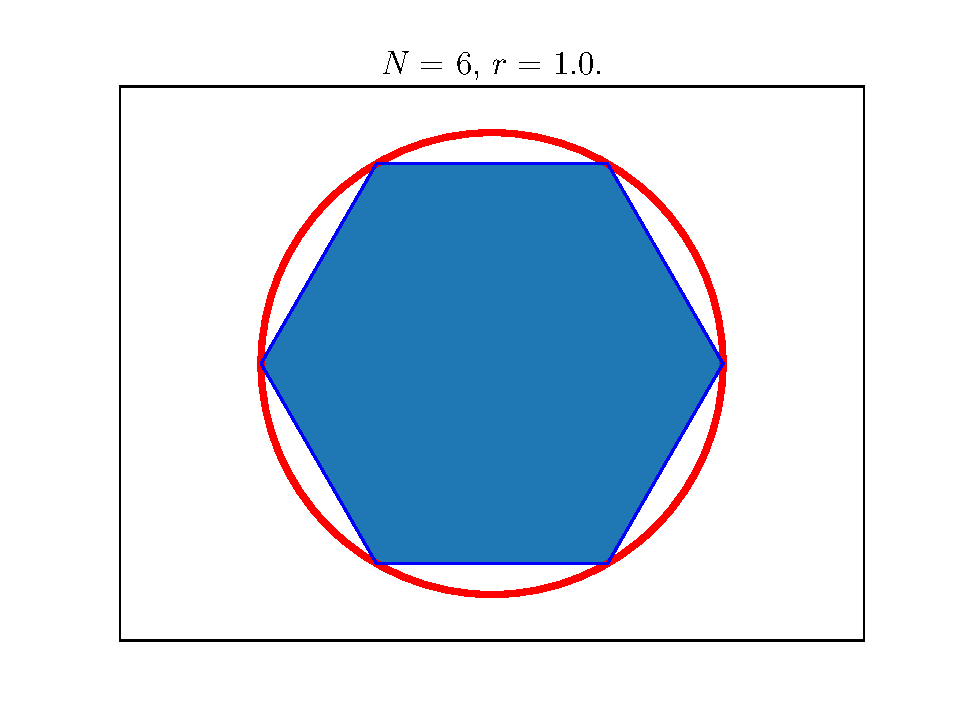
\includegraphics[width=3.1 in]{figuras/complexo/figura_pi.pdf}
\label{figura_pi}
}
\subfigure{b)
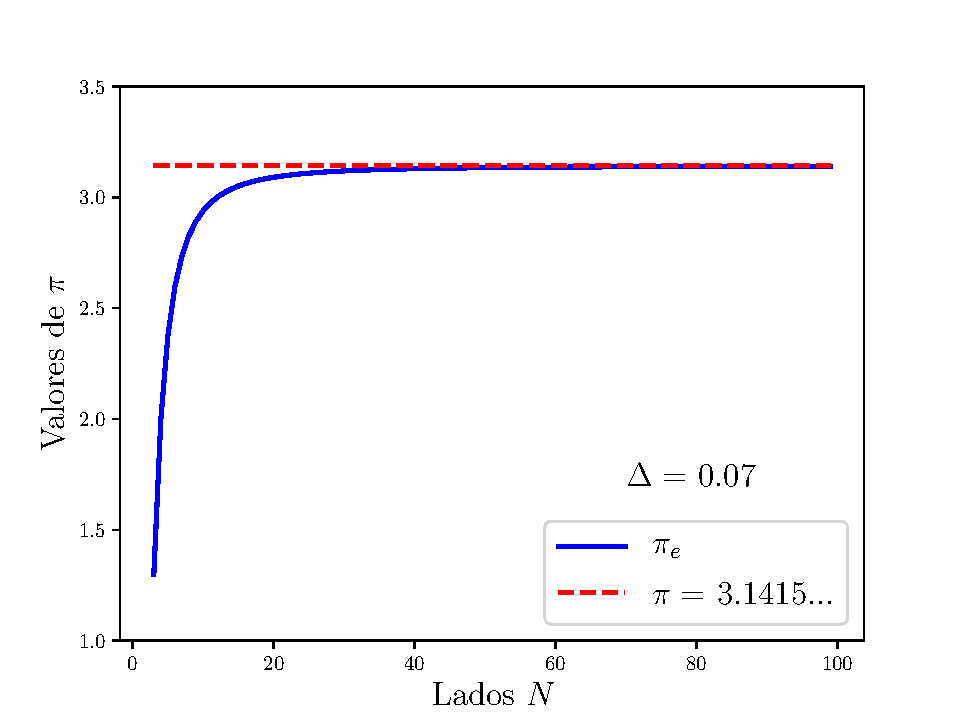
\includegraphics[width=3.1 in]{figuras/complexo/figura_pi2.pdf}
\label{figura_pi2}
}
\caption[C�lculo num�rico do n�mero $\pi$.]{\subref{figura_pi} Hex�gono inscrito em um c�rculo. \subref{figura_pi2} Estimativa $\pi_e$ em fun��o do n�mero de lados $N$. A linha tracejada vermelha � o valor real de $\pi$. O valor $\Delta$ indicado � o erro relativo em porcentagem.}
\end{figure}

\subsection{S�ries de Fun��es}

Quando cada termo de uma s�rie � uma fun��o $u_n = u_n(x)$, trata-se de uma s�rie de fun��es, o que � amplamente utilizado em f�sica. Dessa forma, tanto a soma parcial quanto o limite ficam tamb�m dependentes de $x$. Se para qualquer valor $\varepsilon >0$ existir um $N$ independente de $x$ no intervalo $[a,b]$ tal que:
\begin{equation}
\vert S(x) - s_n(x) \vert < \varepsilon, \qquad \text{para todo } \quad n \geq N,
\end{equation}
dizemos que a s�rie � uniformemente convergente no intervalo $a \leq x \leq b$. Sendo uniformemente convergente uma s�rie de fun��es converge para uma fun��o cont�nua, sendo inclusive diferenci�vel. O intervalo deve ser fechado: incluso os pontos das borda.

As s�ries uniformemente convergentes e com os termos $u_n(x)$ cont�nuos tem tr�s propriedades importantes (muito utilizadas na f�sica):
\begin{itemize}
\item A soma $f(x) = \sum_{n=1}^{\infty} u_n(x)$ tamb�m � cont�nua.
\item A s�rie pode ser integrada termo a termo. A soma das integrais � igual a integral da soma:
\begin{equation}
\int_a^b f(x) dx = \sum_{n=1}^{\infty} \int_a^b u_n(x) dx. \nonumber
\end{equation}
\item A derivada da soma � igual a soma das derivadas:
\begin{equation}
\dfrac{d}{dx} f(x) = \sum_{n=1}^{\infty} \dfrac{d}{dx} u_n(x) . \nonumber
\end{equation}
caso $du_n/dx$ tamb�m seja cont�nuo em $[a,b]$.
\end{itemize}

\subsection{Expans�o de Taylor}

Expans�o de Taylor � uma s�rie de fun��es envolvendo a derivada de uma fun��o com o objetivo de obter uma express�o aproximada para a mesma. Seja $f(x)$ uma fun��o com sua derivada n-�sima $f^{(n)}(x)$ cont�nua no intervalo $a \leq x \leq b$. Integrando essa n-�sima derivada obtemos:
\begin{equation}
\int_a^x f^{(n)}(x) dx_1 = f^{(n-1)}(x_1)\bigg\vert_a^x = f^{(n-1)}(x) - f^{(n-1)}(a). \nonumber
\end{equation}
Integrando novamente:
\begin{eqnarray}
\int_a^x dx_2 \int_a^{x_2} dx_1 f^{(n)}(x_1)  &=& \int_a^x dx_2 \left[ f^{(n-1)}(x_2) - f^{(n-1)}(a) \right], \nonumber \\
&=& f^{(n-2)}(x) - f^{(n-2)}(a) - (x-a)f^{(n-1)}(a). \nonumber
\end{eqnarray}
Mais uma vez:
\begin{equation}
\int_a^x dx_3 \int_a^{x_3} dx_2 \int_a^{x_2} dx_1 f^{(n)}(x_1) = f^{(n-3)}(x) - f^{(n-3)}(a) - (x-a)f^{(n-2)}(a) - \dfrac{(x-a)^2}{2!} f^{(n-1)}(a). \nonumber
\end{equation}
Finalmente, integrando pela n-�sima vez:
\begin{eqnarray}
\int_a^x dx_n \cdot \cdot \cdot \int_a^{x_2} dx_1  f^{(n)}(x_1) = f(x) - f)(a) -  (x-a)f'(a) - \dfrac{(x-a)^2}{2!} f''(a) \nonumber \\
 -\cdot \cdot \cdot - \dfrac{(x-a)^{n-1}}{(n-1)!} f^{(n-1)}(a) . \nonumber
\end{eqnarray}
Estas express�es s�o exatas: n�o cont�m nenhuma aproxima��o. Agora vamos isolar $f(x)$ da �ltima express�o:
\begin{equation}
f(x) = f(a) + (x-a)f'(a) + \dfrac{(x-a)^2}{2!} f''(a) + \cdot \cdot \cdot +  \dfrac{(x-a)^{n-1}}{(n-1)!} f^{(n-1)}(a) + R_n, \nonumber
\end{equation}
onde o �ltimo termo $R_n$ � chamado de restante e � igual a 
\begin{equation}
R_n = \int_a^x dx_n  \cdot \cdot \cdot \int_a^{x_3} dx_1 f^{(n)}(x_1). \nonumber
\end{equation}
Quando este restante tende a zero\footnote{$\lim_{n \rightarrow \infty} R_n = 0$.}, temos a chamada Expans�o de Taylor:
\begin{eqnarray}
f(x) &=& f(a) + (x-a)f'(a) + \dfrac{(x-a)^2}{2!} f''(a)  +  \dfrac{(x-a)^3}{3!} f'''(a) + ... \\ \nonumber
&=& \sum_{n=0}^{\infty} \dfrac{(x-a)^n}{n!} f^{(n)}(a). \nonumber
\end{eqnarray}
A Expans�o de Taylor relaciona o valor da fun��o em um ponto $x$ com o valor de suas derivadas em um ponto de refer�ncia $a$. � uma fun��o na pot�ncia da diferen�a $\Delta = x-a$. Esta expans�o � �til quando se deseja encontrar o valor da fun��o na vizinha�a de um ponto conhecido. Outra forma de se escrever �:
\begin{equation}
f(x+h) = \sum_{n=0}^{\infty} \dfrac{h^n}{n!} f^{(n)}(a), \nonumber
\end{equation}
com $h$ pequeno.

Quando a expans�o � feita em torno de $a=0$, ela � chamada de s�rie de Maclaurin:
\begin{equation}
f(x) = f(0) + xf'(0) + \dfrac{x^2}{2!} f''(0)  +  \dfrac{x^3}{3!} f'''(0) + ... = \sum_{n=0}^{\infty} \dfrac{x^n}{n!} f^{(n)}(0). \nonumber
\end{equation}

\begin{exemplo}
Seja $f(x) = e^x$. Encontre a expans�o de Taylor.
\tcblower
Temos que $f^{(n)}(0) = 1$ para todo $n$ inteiro. Logo:
\begin{equation}
e^x = 1 + x + \dfrac{x^2}{2!} + \dfrac{x^3}{3!} + ... = \sum_{n=0}^{\infty} \dfrac{x^n}{n!}. \nonumber 
\end{equation}
Aplicando o teste da raz�o temos que:
\begin{equation}
\dfrac{a_{n+1}}{a_n}=\dfrac{x^{n+1} n!}{x^n (n+1)!} = \dfrac{x}{n+1} \rightarrow 0 \nonumber
\end{equation}
se $n \rightarrow \infty$. Logo de fato a s�rie � convergente.

Por completeza, vamos calcular o restante $R_n$. Por�m antes vamos reescrev�-lo de outra forma mais conveniente. O teorema do valor m�dio diz que:
\begin{equation}
\int_a^x g(x) dx = (x-a) g(\xi), \nonumber
\end{equation}
para algum $\xi$ tal que $a \leq \xi \leq x$. Integrando $n$ vezes encontramos a forma de Lagrange para o restante:
\begin{equation}
R_n = \dfrac{(x-a)^n}{n!} f^{(n)} (\xi). \nonumber
\end{equation}
Para o caso da exponencial o restante fica:
\begin{equation}
R_n = \dfrac{x^n}{n!} f^{(n)} (\xi) = \dfrac{x^n}{n!} e^{\xi}, \qquad 0 \leq \vert \xi \vert \leq x. \nonumber
\end{equation}
Logo $\vert R_n \vert \leq x^n e^x / n!$, o que implica $\lim_{n\rightarrow \infty} R_n = 0$ para todos os valores finitos de $x$. Logo a s�rie de Maclaurin de $e^x$ converge absolutamente no intervalo $- \infty < x < \infty$.
\end{exemplo}



\begin{codigo} \label{coditaylorerfx}
A fun��o erro aparece na solu��o de algumas equa��es diferenciais de difus�o e tamb�m em estat�stica. Sua defini��o �:
\begin{equation}
\erf (x)=\frac{2}{\sqrt{\pi}}\int_0^x e^{-t^2}\,dt
\end{equation}
Algumas de suas propriedades s�o:
\begin{eqnarray}
  \erf(-\infty)=-1, &\quad& \erf(+\infty)=1 \\
  \erf(-x)=-\erf(x), &\quad& \int_0^x e^{-\frac{t^2}{2\sigma^2}}\,dt=\sqrt{\frac{\pi}{2}}\sigma\,\erf\left[\frac{x}{\sqrt{2}\sigma}\right]
\end{eqnarray}
onde o asterisco significa complexo conjugado.
%\[
% \int_0^x e^{-\frac{t^2}{2\sigma^2}}\,dt=\sqrt{\frac{\pi}{2}}\sigma\,\erf\left[\frac{x}{\sqrt{2}\sigma}\right]
%\]
Apesar de sua defini��o n�o intuitiva, a fun��o erro pode ser aproximada utilizando s�ries de Taylor:
\begin{equation}
g(x) = \sum_{q=0}^{\infty} g_q(x) = \frac{2}{\sqrt{\pi}}  \sum_{q=0}^{\infty} \dfrac{(-1)^q x^{2q+1}}{q!(2q+1)}. \label{seritaylorfuncerroskl}
\end{equation}
onde $g_q(x)$ � a expans�o contendo $q$ termos. Quando a fun��o � complicada, como a fun��o erro, o c�lculo da s�rie de Taylor pode ser trabalhoso. Por�m, isso pode ser facilmente feito utilizando a computa��o simb�lica. Em Python o m�dulo Sympy (\url{http://www.sympy.org}) implementa computa��o simb�lica de maneira simples permitindo a defini��o literal de fun��es diversas e suas opera��es como derivadas (necess�rio para o c�lculo da s�rie de Taylor). Na figura \ref{serie_taylor_erf} est� o gr�fico contendo $\erf (x)$\footnote{O m�dulo SciPy cont�m uma implementa��o da fun��o erro: \url{https://docs.scipy.org/doc/scipy-0.14.0/reference/generated/scipy.special.erf.html}.} e 4 s�ries $g_q(x)$ para $q=$ 1, 11, 21 e 31. O c�digo efetua de forma anal�tica as derivadas para obter as express�es para $g_q(x)$ para qualquer fun��o $f(x)$ que possa ser definida no Sympy.
\end{codigo}

\subsection{S�ries de pot�ncias}

S�ries de pot�ncias aparecem muito em f�sica e por isso merecem uma aten��o em mais detalhes. Sua express�o geral �:
\begin{equation}
f(x) = a_0 + a_1(x-x_0) + a_2(x-x_0)^2 + a_3 (x-x_0)^3 + ... = \sum_{n=0}^{\infty} a_n (x-x_0)^n, \nonumber
\end{equation}
onde os coeficientes $a_n$ s�o independente de $x$ e $x_0$ � uma constante. Sua converg�ncia depende tamb�m do valor de $x$ e pode ser avaliada usando o teste da raz�o:
\begin{equation}
\rho = \lim_{n \rightarrow \infty} \left\vert \dfrac{a_{n+1}(x-x_0)^{n+1}}{a_n(x-x_0)^n} \right\vert. \nonumber
\end{equation}
Se $\rho <1$ a s�rie � convergente.



Um resultado que torna a s�rie de pot�ncia muito �til\footnote{E que pode ser provado pelo teste de Weierstrass.} � o fato de que se ela � convergente para algum $\vert x \vert < R$ ent�o ela � absoluta e uniformemente convergente para para algum intervalo $\vert x \vert <S$ sendo que $0<S<R$. Neste caso, como os termos $a_nx^n$ s�o cont�nuos, a fun��o $f(x)$ tamb�m ser� cont�nua. Logo $f(x)$ � diferenci�vel e integr�vel quantas vezes for desejado. Estas caracter�sticas tornam a s�rie de pot�ncias muito usada em f�sica.

\begin{exemplo}
Avalie se as seguintes s�ries s�o onverentes ou n�o:
\begin{equation}
\text{a)} \quad \sum_{n=0}^{\infty} \dfrac{(-x)^n}{2^n}, \qquad \text{b)} \quad \sum_{n=0}^{\infty} \dfrac{(x+2)^n}{\sqrt{n+1}}. \nonumber
\end{equation}
\tcblower
a) Para a primeira s�rie temos:
\begin{equation}
\rho_n = \left\vert \dfrac{a_{n+1}(x-x_0)^{n+1}}{a_n(x-x_0)^n} \right\vert = \left\vert \dfrac{(-x)^{n+1}}{2^{n+1}} \dfrac{2^n}{(-x)^n} \right\vert = \left\vert \dfrac{x}{2} \right\vert.
\end{equation}
Fazendo o limite $n \rightarrow \infty$ obtemos $\rho = x/2$. Temos ent�o que a s�rie � convergente para $\rho <1$, ou $\vert x \vert < 2$. 

b) Para a segunda s�rie:
\begin{eqnarray}
\rho_n &=& \left\vert \dfrac{(x+2)^{n+1}}{\sqrt{n+2}} \dfrac{\sqrt{n+1}}{(x+2)^n} \right\vert = (x+2) \dfrac{\sqrt{n+1}}{\sqrt{n+2}}, \nonumber \\
\rho &=& \vert x + 2 \vert. \nonumber
\end{eqnarray}
A s�rie converge para $\vert x + 2 \vert < 1$, ou $-3 < x < -1$. Por�m, se $x=-3$ temos a s�rie:
\begin{equation}
1 - \dfrac{1}{\sqrt{2}}+\dfrac{1}{\sqrt{3}} - \dfrac{1}{\sqrt{4}} + \cdot \cdot \cdot \nonumber
\end{equation}
que � convergente. J� para $x=-1$ a s�rie n�o converge. Logo o intervalo de converg�ncia � $-3 \leq x < -1$.
\end{exemplo}




\begin{exemplo} \label{exemplounicidadeseripotendkl}
Mostre que a representa��o em s�rie de pot�ncias de uma fun��o � �nica.
\tcblower
Seja uma fun��o representada por duas s�ries de pot�ncias:
\begin{eqnarray}
f(x)  &=& \left\{
\begin{array}{rl}
\sum_{n=0}^{\infty} a_n x^n& \quad -R_a < x < R_a  \\
\\
 \sum_{n=0}^{\infty} b_n x^n& \quad -R_b < x < R_b
\end{array} 
 \right.
 \nonumber  
\end{eqnarray}
com intervalos coincidentes de converg�ncia, incluindo a origem. Queremos mostrar que $a_n = b_n$ para todo $n$. Dado a defini��o de $f(x)$ podemos escrever:
\begin{equation}
\sum_{n=0}^{\infty} a_n x^n = \sum_{n=0}^{\infty} b_n x^n, \qquad \qquad -R<x<R, \label{seriespotenunicall}
\end{equation}
onde $R$ � o menor entre $R_a$ e $R_b$. Fazendo $x=0$ na Eq. \ref{seriespotenunicall} obtemos $a_0=b_0$. Como � uma s�rie de pot�ncia convergente, vamos derivar a Eq. \ref{seriespotenunicall}:
\begin{equation}
\sum_{n=0}^{\infty} na_n x^{n-1} = \sum_{n=0}^{\infty} nb_n x^{n-1}, \label{seriepotenunica33}.
\end{equation}
Fazendo $x=0$ nesta equa��o obtemos $a_1 = b_1$. Derivando a Eq. \ref{seriepotenunica33} e fazendo $x=0$ obtemos $a_2=b_2$. Repetindo esse processo $n$ vezes obtemos $a_n=b_n$, o que mostra que as duas s�ries coincidem. Assim a representa��o em s�rie de pot�ncias � �nica.
Esta propriedade � essencial na busca de solu��o em s�ries de pot�ncias de equa��es diferenciais.
\end{exemplo}

\subsubsection{Obten��o para s�ries de pot�ncias}

Como s�ries de pot�ncias s�o muito �teis em f�sica, apresentamos aqui alguns dos resultados mais usados e t�cnicas para encontrar outros casos n�o t�o comuns. Por exemplo, as seguintes de fun��es trigonom�tricas e exponenciais s�o predominante em f�sica:
\begin{eqnarray}
\sin x &=& \sum_{n=0}^{\infty} \dfrac{(-1)^n x^{2n+1} }{(2n+1)!} = x - \dfrac{x^3}{3!} + \dfrac{x^5}{5!} - \dfrac{x^7}{7!} + ..., \quad \forall x, \label{seriepotencialseno} \\
\cos x &=& \sum_{n=0}^{\infty} \dfrac{(-1)^n x^{2n} }{(2n)!} = 1 - \dfrac{x^2}{2!} + \dfrac{x^4}{4!} - \dfrac{x^6}{6!} + ..., \quad \forall x, \nonumber \\
e^x &=& \sum_{n=0}^{\infty} \dfrac{ x^n }{n!} =1+ x + \dfrac{x^2}{2!} + \dfrac{x^3}{3!} +  \dfrac{x^4}{4!} + ..., \quad \forall x, \label{seriepoenexponen} \\
\ln (1+x)  &=& \sum_{n=1}^{\infty} \dfrac{ (-1)^{n+1} x^n }{n} = x - \dfrac{x^2}{2!} + \dfrac{x^3}{3!} -  \dfrac{x^4}{4!} + ..., \quad -1< x \leq 1, \label{seriepotencialnwmax}
\end{eqnarray}

V�rias t�cnicas de combina��es de s�ries podem ser usadas para obten��o de s�ries de fun��es aparentemente dif�cieis.

\begin{exemplo}
Ache a s�rie de pot�ncia das seguintes fun��es:
a) $f(x) = (x+1) \sin x$. Usando a Eq. \ref{seriepotencialseno} temos:
\begin{equation}
f(x) = (x+1) \sum_{n=0}^{\infty} \dfrac{(-1)^n x^{2n+1} }{(2n+1)!} = x + x^2 - \dfrac{x^3}{3!} - \dfrac{x^4}{3!} + ... \nonumber
\end{equation} 
b) $f(x) = \dfrac{1}{x} \ln (1+x)$. Divida a Eq. \ref{seriepotencialnwmax} por $x$.

c) $f(x) = e^{-x^2}$. Troque $x$ por $-x^2$ na Eq. \ref{seriepoenexponen}:
\begin{equation}
e^{-x^2} = 1 - x^2 + \dfrac{x^4}{2!} - \dfrac{x^6}{3!}+... \nonumber
\end{equation}
d) $f(x) = \arctan x$. Para essa vamos usar a express�o integral do $\arctan$, Eq. \ref{intearctangelslkj}, e tamb�m a expans�o binomial do integrando. Temos que:
\begin{equation}
\dfrac{1}{1+t^2} = 1 - t^2 + t^4 - t^6 + ... \nonumber
\end{equation}
Logo:
\begin{eqnarray}
\arctan x &=& \int_0^x \dfrac{dt}{1+t^2} = \int_0^x ( 1 - t^2 + t^4 - t^6 + ...)dt =\left(  t - \dfrac{t^3}{3} + \dfrac{t^5}{5} - \dfrac{t^7}{7} + ...\right)\bigg\rvert_0^x, \nonumber \\
&=& x - \dfrac{x^3}{3} + \dfrac{x^5}{5} - \dfrac{x^7}{7} + \cdot \cdot \cdot . \nonumber 
\end{eqnarray}
\end{exemplo}

Veja que esses m�todos s�o mais f�ceis do que tirar v�rias derivadas de $f(x)$. E o teorema deduzido no exemplo \ref{chapseriescomplexos}.\ref{exemplounicidadeseripotendkl} assegura que se encontrarmos uma solu��o, essa � a solu��o.

\begin{figure}[!h]
\centering
\subfigure{a)
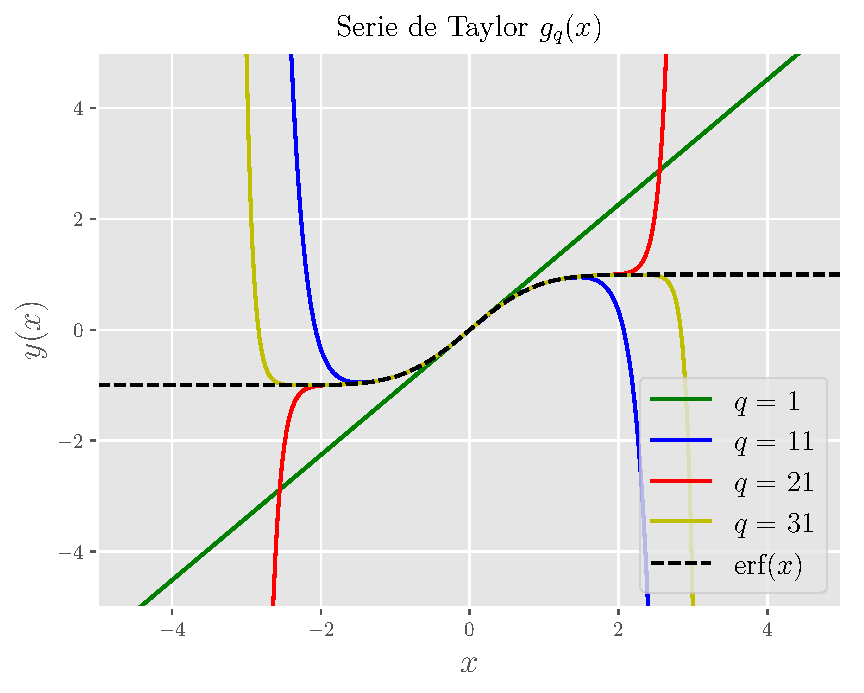
\includegraphics[width=3.2 in]{figuras/complexo/serie_taylor_erf.pdf}
\label{serie_taylor_erf}
}
\subfigure{b)
\includegraphics[width=2.4 in]{figuras/complexo/tijolos.png}
\label{tijolos}
}
\caption[S�ries.]{\subref{serie_taylor_erf} Gr�fico da fun��o erro $\erf(x)$ e suas expans�es de Taylor $g_q(x)$ com $q =$ 1, 11, 21 e 31. \subref{tijolos} Pilha de tijolos. Geometria referente ao problema \ref{chapseriescomplexos}.\ref{rpopilhadetijolos}.}
\end{figure}


%\begin{SCfigure}
%\centering
%\includegraphics[width=2.9 in]{figuras/complexo/tijolos.png}
%\caption{ Pilha de tijolos. Geometria referente ao problema \ref{chapseriescomplexos}.\ref{rpopilhadetijolos}.} 
%\label{tijolos}
%\end{SCfigure}




{\noindent\def\stackalignment{l}% code from https://tex.stackexchange.com/a/195118/101651
    \stackunder[0pt]{\colorbox{cyan}{\textcolor{white}{\textbf{\LARGE Problemas}}}}{\textcolor{lightcyan}{\rule{\linewidth}{2pt}}}\medskip}
    

\begin{problema}
Prove o resultado \ref{somedosprnsldkje} por indu��o. a) Prove que vale para $n=1$. b) Prove que se vale para $n$, vale tamb�m para $n+1$. c) Usando este resultado, mostre que d�zimas peri�dicas infinitas podem ser escritas como fra��es, por exemplo: 1,1111... = 10/9 e 0.131313... = 13/99.
\end{problema}

\begin{problema} \label{coeficbinomiskais}
Seja $f(x) = (1+x)^m$. a) Mostre que:
\begin{equation}
f(x) = 1 + mx + \dfrac{m(m-1)}{2!}x^2 + \dfrac{m(m-1)(m-2)}{3!}x^3+ ... \nonumber
\end{equation}
b) Os coeficientes binomiais $B_{mn}$ s�o definidos como os coeficientes na expans�o:
\begin{equation}
(1+x)^m = \sum_{n=0}^{+\infty} B_{mn} x^n. \nonumber
\end{equation}
Calcule $B_{mn}$.
\end{problema}

\begin{problema}
A raz�o de duas fun��es $g(x)$ e $f(x)$ � indeterminada quando ambas as fun��es tendem para zero quando $x \rightarrow x_0$. Prove a regra de l'Hopital:
\begin{equation}
\lim_{x \rightarrow x_0} \dfrac{g(x)}{f(x)} = \lim_{x \rightarrow x_0} \dfrac{g'(x)}{f'(x)}. \nonumber 
\end{equation}
\end{problema}


\begin{problema}
Encontre o limite para $n \rightarrow \infty$ das seguintes sequ�ncias:
\begin{eqnarray}
\text{a)} \quad a_n &=& \dfrac{n^2 + 5n^3}{2n^3 + 3\sqrt{4+n^6}}, \qquad \text{b)} \quad b_n = \dfrac{(n+1)^2}{\sqrt{3+5n^2+3n^3}}, \nonumber \\
\text{c)} \quad c_n &=& \dfrac{3^n}{n^2}, \qquad \text{d)} \quad d_n = n \cos (1/n). \nonumber 
\end{eqnarray}
\end{problema}

\begin{problema}
Deduza a F�rmula de Euler: $e^{ix} = \cos x + i \sin x$.
\end{problema}

\begin{problema}
Usando os m�todos da se��o, calcule a expans�o em s�rie das fun��es:
\begin{eqnarray}
\text{a)} \quad f(x) &=& e^x \cos x, \qquad \text{b)} \quad g(x) = x \sqrt{a+bx},  \nonumber \\
\text{c)} \quad h(x) &=& \cos x^3, \qquad \text{b)} \quad i(x) = \dfrac{x}{\sqrt{a+bx}}.  \nonumber 
\end{eqnarray}
\end{problema}


\begin{problema} \label{hipergeometriagauss}
$\bigstar$ Determine os maiores e os menores valores de $x$, ou seja, o intervalo de converg�ncia da s�rie hipergeom�trica de Gauss:
\begin{equation}
F(\alpha,\beta,\gamma;x) = 1 + \dfrac{\alpha \beta}{1! \gamma}x + \dfrac{ (\alpha+1) (\beta+1)\alpha \beta}{2!\gamma (\gamma+1)}x^2 + ...
\end{equation} 
\end{problema}

\begin{problema} \label{proelmaclaurinlogranauta}
a) Encontre a s�rie de Maclaurin de $f(x) = \ln (1+x)$. b) Encontre a expans�o de Taylo de $e^{\tan x}$. c) Encontre a expans�o de $\arctan x$.
\end{problema}

\begin{problema} \label{erroaproxderivdaseugnda}
Em an�lise num�rica � comum aproximar a derivada segunda por:
\begin{equation}
\dfrac{d^2 \psi}{dx^2} \approx \dfrac{\psi (x+h) -2\psi (x) + \psi(x-h)}{h^2}. \nonumber
\end{equation}
Encontre o erro nesta aproxima��o. 
\end{problema}


\begin{problema} 
A teoria de Planck de osciladores quantizados leva a uma energia m�dia da forma:
\begin{equation}
\langle \varepsilon\rangle = \dfrac{\sum_{n=1}^{\infty} n \varepsilon_0 \exp \left( -n\varepsilon_0/kT\right)   }{\sum_{n=1}^{\infty} \exp \left( -n\varepsilon_0/kT\right) }. \nonumber
\end{equation}
Mostre que:
\begin{equation}
\langle \varepsilon\rangle = \dfrac{\varepsilon_0}{\exp (\varepsilon_0 / kT) -1}. \nonumber
\end{equation}
\end{problema}

\begin{problema}
A teoria cl�ssica de Langevin para o paramagnetismo fornece a a polariza��o magn�tica o seguinte resultado:
\begin{equation}
P(\alpha) = A \left( \dfrac{\cosh \alpha}{ \sinh \alpha} - \dfrac{1}{\alpha } \right), \nonumber
\end{equation}
onde $A$ � uma constante. Expanda $P(\alpha)$ em s�rie de pot�ncias para $\alpha << 1$ (baixo campo e alta temperatura).
\end{problema}

\begin{problema}
{\color{red}\Keyboard} $\bigstar$ a) Mostre que a expans�o de Taylor da fun��o erro � a Eq. \ref{seritaylorfuncerroskl}. b) Quantos termos s�o necess�rios para se obter $\text{erf} (0.1)$, $\text{erf} (1)$ e $\text{erf} (2)$? Use computa��o simb�lica ou escreva um c�digo computacional que resolva numericamente. 
\end{problema}
%
\begin{problema} \label{rpopilhadetijolos}
$\bigstar$ a) Mostre que � poss�vel empilhar tijolos (ou livros) de forma que o tijolo mais alto esteja t�o longe a direita do primeiro quanto voc� queira. Veja figura \ref{tijolos}. b) Encontre a dist�ncia entre a borda da direita do tijolo mais alto para a mesma borda do tijolo abaixo dele. c) Encontre a f�rmula geral para essa dist�ncia para qualquer tijolo da pilha. Dica: Calcule o torque na borda considerando as tr�s for�as atuando no tijolo. d) Mostre que a soma dessas dist�ncias � uma s�rie divergente\footnote{Veja John F. Hall \textit{Fun with stacking blocks}, Am. J. Phys. \href{http://dx.doi.org/10.1119/1.2074007}{\textbf{73}, 1107 (2005)}. Para uma pilha invertida veja M. Paterson, Y. Peres, M. Thorup, P. Winkler and U. Zwick \textit{Maximum Overhang}, The American Mathematical Monthly, \href{http://www.jstor.org/stable/40391297?origin=JSTOR-pdf}{\textbf{116}, No. 9, pp. 763-787 (2009)}.}. 
\end{problema}


\begin{problema} \label{cladogipinumeriosl}
{\color{red}\Keyboard} A �rea de um pol�gono regular de $N$ lados pode ser calculado considerando o pol�gono como uma soma de tri�ngulos. Dado um sistema de coordenadas, esta �rea pode ser encontrada em fun��o das coordenadas $x,y$ de cada v�rtice atrav�s da F�rmula do Cadarso\footnote{Ou f�rmula da �rea de Gauss, pois foi desenvolvida de maneira independente por Meister em 1769 e por Gauss (sempre ele) em 1795. Veja por exemplo \url{https://en.wikipedia.org/wiki/Shoelace_formula}.}:
\begin{equation}
A(N) =  \dfrac{1}{2} \sum_{i=1}^N (x_iy_{i+1} - x_{i+1}y_i), \nonumber
\end{equation}
onde $x_i,y_i$ s�o as coordenadas do i-�simo ponto. � necess�rio que os pontos sejam ordenados: $x_0,y_0$ � o primeiro, $x_1,y_1$ o segundo, etc...
a) Fa�a um pseudo-algoritmo que calcule numericamente a estimativa $\pi_e(N)$ para um pol�gono de $N$ lados (veja Eq. \ref{slekjfwoislkjppp}), usando o m�todo do c�digo \ref{chapseriescomplexos}.\ref{codigopinumericos} e a F�rmula do Cadarso. b) A partir desse algoritmo, desenvolva uma implementa��o em Python que fa�a o c�lculo e gere os gr�ficos como das figuras \ref{figura_pi} e \ref{figura_pi2}.
\end{problema}

%\begin{problema} 
%{\color{red}\Keyboard} Use o c�digo que gera a figura \ref{serie_taylor_erf} referente ao exemplo \ref{chapseriescomplexos}.\ref{coditaylorerfx} e obtenha a expans�o de Taylor para 4 valores diferentes de $q$ para as seguintes fun��es: a) 
%\end{problema}

\begin{problema}
$\bigstar \bigstar \quad$ Mostre que:
\begin{equation}
\int_0^{\infty} \dfrac{\sinh (\pi x) }{\sinh (3\pi x)} e^{-3\pi x^2} dx = \dfrac{1}{\sqrt{3} e^{2\pi /3}} \sum_0^{\infty} \dfrac{\exp \left[ -2n(n+1)\pi \right] }{(1+e^{-\pi})^2 (1+e^{-3\pi})^2 \cdot \cdot \cdot (1+e^{-(2n+1)\pi})^2 } . \nonumber
\end{equation}
Dica: veja \cite{Nahin2015}.
\end{problema}

\begin{problema}
$\bigstar \bigstar \quad$ Mostre os seguintes resultados:
\begin{eqnarray}
\text{a)} \quad \int_0^1 x^x dx &=& 1 - \dfrac{1}{2^2} + \dfrac{1}{3^3} - \dfrac{1}{4^4} + \dfrac{1}{5^5} - ... = 0.78343... \label{irresistivelinte1} \\
\text{b)} \quad \int_0^1 x^{x^2} dx &=& 1 - \dfrac{1}{3^2} + \dfrac{1}{5^3} - \dfrac{1}{7^4} + \dfrac{1}{9^5} - ... = 0.89648... \nonumber \\
\text{c)} \quad \int_0^1 x^{\sqrt{x}} dx &=& 1 - \left(  \dfrac{2}{3} \right)^2  + \left(  \dfrac{2}{4} \right)^3 - \left(  \dfrac{2}{5} \right)^4  + \left(  \dfrac{2}{6} \right)^5 - ... = 0.65858... \nonumber
\end{eqnarray}
A integral da Eq. \ref{irresistivelinte1} foi resolvida primeiramente pelo matem�tico sui�o John Bernoulli em 1697. Ele ficou t�o fascinado pelo resultado que o chamou de "series mirabili", ou s�rie maravilhosa\footnote{Veja Ref. \cite{Nahin2015}.}. 
\end{problema}

\begin{problema}
Se voc� fizer um investimento com juros compostos de 5 \% ao m�s, voc� ter� $(1.005)^n$ reais ap�s $n$ meses. Se voc� investir 30 reais no in�cio de cada m�s, quanto voc� ter� ao final de 15 anos? 
\end{problema}


{\noindent\def\stackalignment{l}{\textcolor{lightcyan}{\rule{\linewidth}{2pt}}}\medskip}


\section{N�meros Complexos}


N�meros complexos s�o formados por um par de n�meros reais de forma que o conjunto dos reais $\mathbb{R}$ faz parte do conjunto dos complexos $\mathbb{C}$. Em geral, fun��es e s�ries reais podem ser generalizadas para complexas apenas trocando as vari�veis reais por complexas. 

N�meros complexos s�o usados em f�sica por exemplo na solu��o de equa��es diferenciais e tamb�m na descri��o dos campos el�trico e magn�tico.

\subsection{�lgebra Complexa}

A primeira e mais simples motiva��o para a defini��o dos n�meros complexos � a solu��o de equa��es quadr�ticas.

\begin{exemplo}
Seja $y(x) = x^2 + x +1$ para $x\in \mathtt{R}$ ($x$ real). Encontre as solu��es para $y(x)=0$.
\tcblower
Usando a f�rmula de Baskara e delta verifica-se que n�o h� solu��o real. Por�m, se usarmos o s�mbolo $i = \sqrt{-1}$ podemos encontrar solu��es. De fato, verifica-se que $x_{\pm} = \frac{1}{2} (-1 \pm i \sqrt{3})$ � solu��o:
\begin{equation}
\left[ \dfrac{1}{2} (-1 \pm i\sqrt{3} \right]^2 + \dfrac{1}{2}(-1 \pm i \sqrt{3}) +1 = \dfrac{1}{4} (1 -3 \mp 2i \sqrt{3} -2 \pm 2i \sqrt{3}) + 1 = 0. \nonumber 
\end{equation}
Matematicamente o problema foi resolvido, por�m ainda n�o temos um significado para o s�mbolo $i$.
\end{exemplo} 

Para formalizar mais a exist�ncia desses n�meros complexos definimos o chamado plano complexo formado pelos eixos $x$ e $y$ (veja figura \ref{plano_complexo}). Assim cada n�mero complexo ser� definido pelo par $z \equiv (x,y)$ onde $x$ � chamado de parte real $\operatorname{Re}(z)$ e $y$ a parte imagin�ria $\operatorname{Im}(z)$: 
\begin{equation}
z \equiv (x,y) = x + iy, \qquad \qquad x = \operatorname{Re}(z), \qquad \qquad y = \operatorname{Im}(z). \nonumber
\end{equation}
Dessa forma, um n�mero real � escrito como $(x,0)$ a unidade imagin�ria � definida como $i \equiv (0,1)$\footnote{Em outras �reas, engenharia por exemplo, � comum usar $j$ como sendo a unidade imagin�ria.}.

%\begin{SCfigure}
% \centering
%\begin{tikzpicture}
%\begin{axis}
%    [
%    ytick ={-2, 0, 2,3}, yticklabels={$-2i$, $0$, $2i$, $3i$},
%    axis lines = center,
%    %grid=both,
%    minor tick num=1,
%    ticks=both,
%    xlabel=$x$,
%    ylabel=$y$,
%    ymin=-3,
%    ymax=+4,
%    xmin=-4,
%    xmax=+5
%    ]
%
%    \addplot [blue, mark = *] coordinates {( 0, 0)} {};
%    \addplot [blue, mark = *] coordinates {( 3, 2)} {};
%    \addplot [blue, mark = *] coordinates {( 2, 3)} {};
%    \addplot [blue, mark = *] coordinates {( -1, 1)} {};
%
%    \node [below right, red] at (axis cs:  0, 0) {};
%    \node [right, red] at (axis cs:  3, 2) {$3+2i$};
%    \node [above, red] at (axis cs:  2, 3) {$2+3i$};
%    \node [left, red] at (axis cs:  -1, 1) {$-1+i$};
%
%%    \addplot [dashed, black] coordinates { (0,0) (3,2) };
%%    \addplot [dashed, black] coordinates { (3,2) (2,3) };
%%    \addplot [dashed, black] coordinates { (2,3) (-1,1) };
%%    \addplot [dashed, black] coordinates { (-1,1) (0,0) };
%
%\end{axis}
%\end{tikzpicture}
%\caption{Plano complexo com alguns pontos representados.}
%\label{plano_complexo}
%\end{SCfigure} 

Um n�mero complexo $z=(a,b)$ nada mais � ent�o do que um ponto no plano complexo, tendo sua abcissa como a parte real e a ordenada como a parte imagin�ria. Toda a an�lise envolvendo n�meros complexos � feita baseando nos pares ordenados. A soma por exemplo �:
\begin{equation}
z_1+z_2 = (x_1,y_1) + (x_2,y_2) = (x_1+x_2,y_1+y_2) = z_1+z_2. \nonumber
\end{equation}
Veja que $x$ e $y$ se comportam como coordenadas de um vetor $z$ no plano complexo. A multiplica��o fica:
\begin{equation}
z_1z_2 = (x_1+iy_2)(x_2+iy_2) = x_1x_2 -y_1y_2 + i(x_1y_2 + x_2y_1). \nonumber
\end{equation}
Lembrando que $i^2 = -1$.

Outra opera��o muito utilizada na f�sica � o complexo conjugado $z^*$ de um n�mero complexo $z=(a+ib)$, definido como $z^* = a-ib$. Veja que tirar o complexo conjugado significa apenas trocar o sinal da parte imagin�ria. Dessa forma temos:
\begin{equation}
zz^* = (a+ib)(a-ib) = a^2 + b^2 = \vert z \vert,
\end{equation}
onde $\vert z \vert$ � chamado de m�dulo de $z$. 

J� a divis�o de dois n�mero complexos consiste em deixar o denominador real:
\begin{equation}
\dfrac{z_1}{z_2} = \dfrac{z_1}{z_2} \dfrac{z_2^*}{z_2^*} = \dfrac{z_1 z_2^*}{\vert z_2 \vert } 
\end{equation}
Por exemplo, se $z_1 = a_1+ib_1$ e $z_2 = a_2+ib_2$ a divis�o de ambos ser�:
\begin{equation}
\dfrac{z_1}{z_2} = \dfrac{a_1a_2+b_1b_2 + i(a_2b_1-a_1b_2)}{a_2^2+b_2^2}. \label{slsdkjfppqqpa}
\end{equation}


\begin{figure}[!h]
\centering
\subfigure{a)
\begin{tikzpicture}
\begin{axis}
    [
    ytick ={-2, 0, 2,3}, yticklabels={$-2i$, $0$, $2i$, $3i$},
    axis lines = center,
    %grid=both,
    minor tick num=1,
    ticks=both,
    xlabel=$x$,
    ylabel=$y$,
    ymin=-3,
    ymax=+4,
    xmin=-4,
    xmax=+5
    ]

    \addplot [blue, mark = *] coordinates {( 0, 0)} {};
    \addplot [blue, mark = *] coordinates {( 3, 2)} {};
    \addplot [blue, mark = *] coordinates {( 2, 3)} {};
    \addplot [blue, mark = *] coordinates {( -1, 1)} {};

    \node [below right, red] at (axis cs:  0, 0) {};
    \node [right, red] at (axis cs:  3, 2) {$3+2i$};
    \node [above, red] at (axis cs:  2, 3) {$2+3i$};
    \node [left, red] at (axis cs:  -1, 1) {$-1+i$};

%    \addplot [dashed, black] coordinates { (0,0) (3,2) };
%    \addplot [dashed, black] coordinates { (3,2) (2,3) };
%    \addplot [dashed, black] coordinates { (2,3) (-1,1) };
%    \addplot [dashed, black] coordinates { (-1,1) (0,0) };

\end{axis}
\end{tikzpicture}
\label{plano_complexo}
}
\subfigure{b)
\begin{tikzpicture} [thick]
  \draw[thin,gray!40] (-1,-1) grid (4.0,3.0);
  \draw[<->] (-1,0)--(4,0) node[above]{$x$};
  \draw[<->] (0,-1)--(0,3) node[left]{$y$};
  \draw[line width=2pt,blue,-stealth](0,0)--(3,0) node[above]{$x$};
  \draw[line width=2pt,red,-stealth](0,0)--(0,2) node[right]{$y$};
  \draw[line width=2pt,black,-stealth](0,0)--(3,2) node[anchor=south west]{$z$};
  \node[] at (1.3,1.2) {$r$};


\coordinate (O) at (0,0);
\coordinate (A) at (3,0);
\coordinate (B) at (3,2);
%\draw (O)--(A)--(B)--cycle;

\tkzMarkAngle[fill= orange,size=0.8cm,opacity=.4](A,O,B)
\tkzLabelAngle[pos = 0.6](A,O,B){$\theta$}

%\shade[inner color = black, outer color = blue] (0,0) circle (0.1);
%\shade[inner color = black, outer color = red] (5,5) circle (0.1);

\end{tikzpicture}
\label{complexo_polar}
}
\caption{\subref{plano_complexo} Plano complexo com alguns pontos representados. \subref{complexo_polar} Representa��o polar de um n�mero complexo.}
\end{figure}


%
%\begin{SCfigure}
% \centering
%\begin{tikzpicture} [thick]
%  \draw[thin,gray!40] (-1,-1) grid (4.0,3.0);
%  \draw[<->] (-1,0)--(4,0) node[above]{$x$};
%  \draw[<->] (0,-1)--(0,3) node[left]{$y$};
%  \draw[line width=2pt,blue,-stealth](0,0)--(3,0) node[above]{$x$};
%  \draw[line width=2pt,red,-stealth](0,0)--(0,2) node[right]{$y$};
%  \draw[line width=2pt,black,-stealth](0,0)--(3,2) node[anchor=south west]{$z$};
%  \node[] at (1.3,1.2) {$r$};
%
%
%\coordinate (O) at (0,0);
%\coordinate (A) at (3,0);
%\coordinate (B) at (3,2);
%%\draw (O)--(A)--(B)--cycle;
%
%\tkzMarkAngle[fill= orange,size=0.8cm,opacity=.4](A,O,B)
%\tkzLabelAngle[pos = 0.6](A,O,B){$\theta$}
%
%%\shade[inner color = black, outer color = blue] (0,0) circle (0.1);
%%\shade[inner color = black, outer color = red] (5,5) circle (0.1);
%
%\end{tikzpicture}
%\caption{Plano complexo com alguns pontos representados.}
%\label{plano_complexo}
%\end{SCfigure} 


\subsection{Forma polar}

Outra forma �til de escrever n�meros complexos � usando coordenadas polares. Da figura \ref{complexo_polar} temos que:
\begin{equation}
x = r \cos \theta, \qquad y = r \sin \theta, \qquad z = r (\cos \theta + i \sin \theta). \label{mmmmammmm}
\end{equation}
Agora, $r$ e $\theta$ s�o chamados de m�dulo e fase de $z$:
\begin{equation}
r = \sqrt{x^2 + y^2}, \qquad \tan \theta = \dfrac{y}{x}. \nonumber
\end{equation}
Para obtermos uma rela��o �til, vamos expandir a exponencial complexa em uma s�rie:
\begin{eqnarray}
e^{i \theta} &=& \sum_{n=0}^{\infty} \dfrac{(i\theta)^n}{n!} =  \sum_{m=0}^{\infty} \dfrac{(i\theta)^{2m}}{(2m)!} +  \sum_{m=0}^{\infty} \dfrac{(i\theta)^{2m+1}}{(2m+1)!} = \sum_{m=0}^{\infty} (i)^m\dfrac{(\theta)^{2m}}{(2m)!} + i  \sum_{m=0}^{\infty} (-1)^m \dfrac{(\theta)^{2m+1}}{(2m+1)!}, \nonumber \\
&=& \cos \theta + i \sin \theta. \label{slskjwoiwlkjsfdf}
\end{eqnarray}
A Eq. \ref{slskjwoiwlkjsfdf} � a famosa rela��o de Euler. A partir dela podemos representar um n�mero complexo em coordenada polar (Eq. \ref{mmmmammmm}) como $z = r e^{i\theta}$. A f�rmula de Euler permite escrever as regras de adi��o de �ngulos, por exemplo:
\begin{equation}
\cos (\theta_1 + \theta_2) + i \sin (\theta_1 + \theta_2) = \cos \theta_1 \cos \theta_2 - \sin \theta_1 \sin \theta_2 + i (\sin \theta_1 \cos \theta_2 + \sin \theta_2 \cos \theta_1). \label{kkkkwkkkk} 
\end{equation}
Outras propriedades interessante s�o:
\begin{equation}
\vert z_1 \vert - \vert z_2 \vert \leq \vert z_1 + z_2 \vert \leq \vert z_1 \vert + \vert z_2 \vert, \qquad \vert z_1 \cdot z_2 \vert = \vert z_1 \vert \cdot \vert z_2 \vert. \label{wywywhqhqhmm}
\end{equation}


A escolha da representa��o cartesiana ou polar para os n�meros complexos � uma quest�o de conveni�ncia. Soma e subtra��o � mais simples usando cartesianas j� multiplica��o, divis�o e radicia��o s�o mais f�ceis usando a representa��o polar. Por exemplo:
\begin{equation}
\sqrt[n]{z}  = \sqrt[n]{re^{i \theta}} = \sqrt[n]{re^{i \theta+2im\pi}} = \sqrt[n]{r} \exp{i \theta /n + 2im\pi /n}, \qquad m = 1,2,3,..., n-1, \nonumber
\end{equation}
j� que, da f�rmula de Euler (Eq. \ref{slskjwoiwlkjsfdf}), $\exp{i\theta + 2im\pi} = e^{i\theta} \cos 2m\pi = e^{i\theta}$. Ou seja, radicia��o de um n�mero complexo � uma fun��o multivalorada (para cada $z$ retorna mais de um resultado).

Outro exemplo de fun��o complexa multivalorada � o logaritmo. Em princ�pio ter�amos $\ln z = \ln r e^{i\theta} = \ln r + i \theta$. Por�m, usando novamente $\exp{i\theta + 2in\pi} = e^{i\theta}$ temos que:
\begin{equation}
\ln z = \ln r \exp{i\theta + 2in\pi} = \ln r + i (\theta + 2n\pi), \qquad n = 0,1,2,3,...
\end{equation}
Ou seja, $\ln z$ pode retornar infinitos valores para cada real $r$ e $\theta$. � comum usar como padr�o $n=0$ e $\theta$ em qualquer intervalo de comprimento $2\pi$ para que $\ln z$ retorne um valor apenas.


\begin{codigo}
S�rie de n�meros complexos tem diversas aplica��es, como por exemplo em fractais. Por exemplo o conjunto de Mandelbrot que � o conjunto $M$ de n�meros complexos $c \in \mathbb{C}$ tais que a s�rie $z_{n+1} = z_n^2 + c$ n�o � divergente, usando $z_0=0$. Dizer que uma s�rie n�o diverge n�o implica que ela converge, mas que o seu valor m�ximo � limitado. Assim, o conjunto $M$ de Maldelbrot � pode ser definido como:
\begin{equation}
c \in \mathbb{M} \Longleftrightarrow \lim_{n \rightarrow + \infty} \vert z_{n+1} \vert \leq L. \label{criconjbmandelbrot}
\end{equation}
� comum usar $L=2$. Para $c=1$ a s�rie $z_n$ diverge. Mas para $c=-1$ a s�rie � convergente logo $-1 \in \mathbb{M}$.

Uma maneira de fazer uma figura mostrando o conjunto $\mathbb{M}$ � definir um dom�nio no plano complexo e ent�o calcular o n-�simo termo $z_n$ para todos os valores de $c$ neste dom�nio. Quando $\vert z_n \vert<2$ , colore-se o ponto $c$ de vermelho, caso contr�rio de branco, como est� na figura \ref{fractal_mandelbrot}. 
%O c�digo que gera esta figura �: \lstinputlisting[language=Python]{figuras/complexo/mandelbrot4.py}
Veja que a fun��o limite retorna 1 se $\vert z_{100} \vert < L=2$ e 0 caso contr�rio. S�o calculados no total $10^6$ valores de $c$ (1000 valores para sua parte real guardadas no vetor x e 1000 para a parte imagin�ria no vetor y). Os valores calculados da fun��o s�o armazenados na matriz \verb|fm|. O gr�fico � feito usando o comando \verb|plt.imshow|.
\end{codigo}


\begin{SCfigure}
\centering
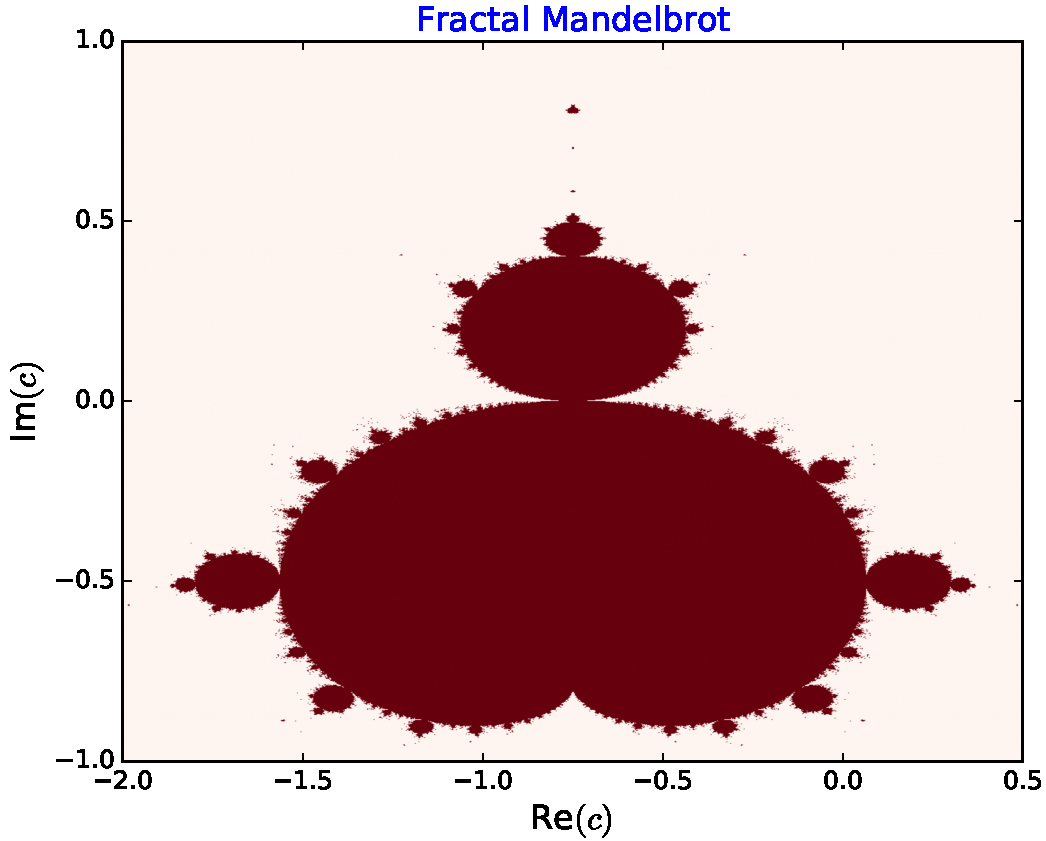
\includegraphics[width=2.8 in]{figuras/complexo/fractal_mandelbrot.pdf}
\caption[Fractal de Mandelbrot.]{Fractal de Mandelbrot.} 
\label{fractal_mandelbrot}
\end{SCfigure}

%\begin{figure}[!h]
%\centering
%\subfigure{a)
%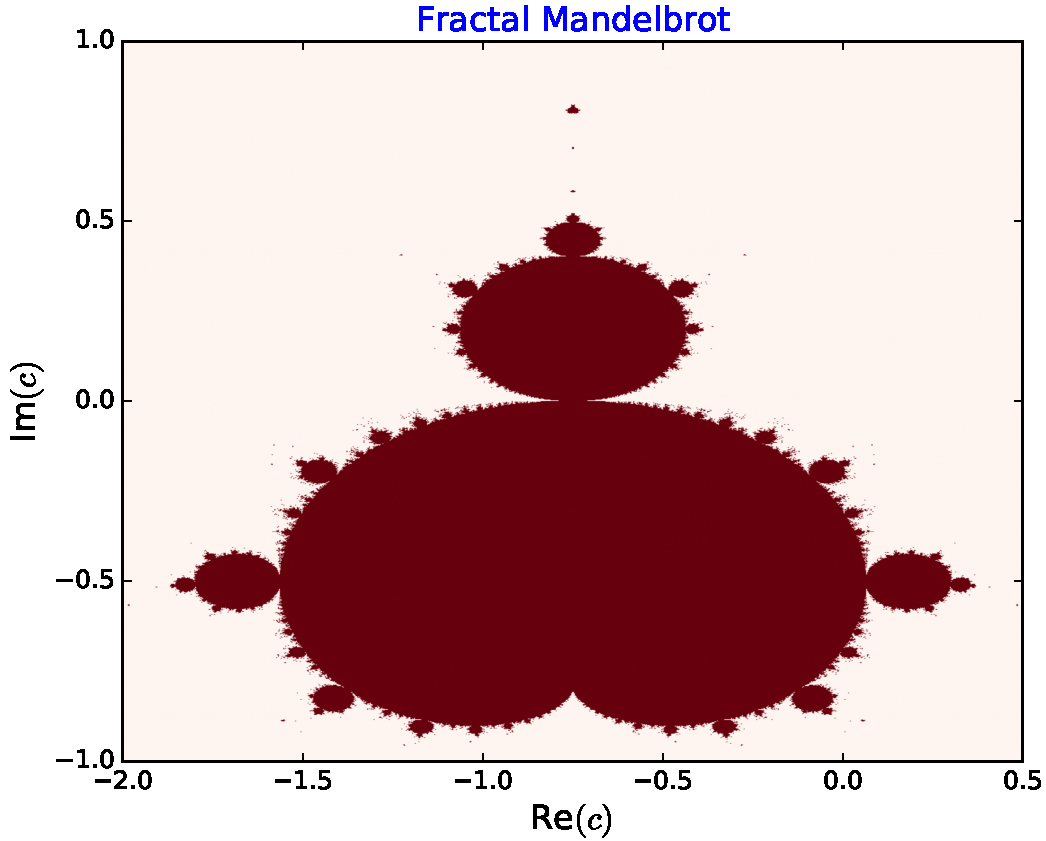
\includegraphics[width=2.8 in]{figuras/complexo/fractal_mandelbrot.pdf}
%\label{fractal_mandelbrot}
%}
%\subfigure{b)
%\includegraphics[width=2.7 in]{figuras/complexo/fractal_mandelbrot2.pdf}
%\label{fractal_mandelbrot2}
%}
%\caption[Fractal de Mandelbrot.]{Fractal de Mandelbrot. \subref{fractal_mandelbrot} Gr�fico simples ilustrando o conceito do algoritmo. \subref{fractal_mandelbrot2} Renderiza��o mais completa. O c�digo est� dispon�vel em \href{https://matplotlib.org/examples/showcase/mandelbrot.html}{https://matplotlib.org/}.}
%\end{figure}




\begin{tcolorbox}[breakable,pad at break*=1mm,colback=blue!5!white,colframe=DarkGreen!75!black,title=Um pouco de hist�ria.]

A matem�tica de fractais come�ou possivelmente no s�culo XVII com o matem�tico e fil�sofo Gottfried Leibniz (o mesmo do c�lculo), quando ele considerou o conceito de similaridade recursiva, usando o termo expoentes fractais. Apenas em 1872 Karl Weierstrass apresentou � Royal Prussian Academy of Sciences uma fun��o que hoje � considerada como fractal tendo a propriedade n�o intuitiva de ser cont�nua em todo o espa�o mas n�o diferenci�vel. Em 1883, Georg Cantor, que assistiu as palestras de Leibniz apresentou o fractal que hoje � conhecido como conjunto de Cantor. Todos os tratamentos at� ent�o eram anal�ticos e apenas em 1904 os primeiros desenhos (feitos a m�o) foram apresentados, relativo ao fractal conhecido como floco de neve. Em 1915 foi apresentado o tri�ngulo de Sierpinski, em 1918 o fractal de Julia (por Pierre Fatou e Gaston Julia de maneira independente, veja a figura \ref{fractal_julia}).

O estudo de fractais deu um grande salto com Benoit Mandelbrot, que criou o fractal q leva seu nome (veja figuras \ref{fractal_mandelbrot} e \ref{fractal_mandelbrot2}) ap�s seus estudos tentando encontrar o comprimento da costa da Gr�-Bretanha. Em 1975 apresentou os primeiros gr�ficos gerados em computador de um fractal, cunhando tamb�m o termo fractal. O fractal de Mandelbrot foi artigo de capa da Scientific American em agosto de 1985 e apresentou ao p�blico geral um algoritmo para cri�-lo.
\end{tcolorbox}


{\noindent\def\stackalignment{l}% code from https://tex.stackexchange.com/a/195118/101651
    \stackunder[0pt]{\colorbox{cyan}{\textcolor{white}{\textbf{\LARGE Problemas}}}}{\textcolor{lightcyan}{\rule{\linewidth}{2pt}}}\medskip}
    


\begin{problema}
a) Deduza a express�o da Eq. \ref{slsdkjfppqqpa}. b) Deduza a equa��o \ref{kkkkwkkkk}. c) Deduza os resultados das equa��es \ref{wywywhqhqhmm}. d) Mostre que $\arg (z_1z_2) = \arg(z_1) + \arg(z_2)$, onde $\arg(z)=$ a fase de $z$.
\end{problema}

\begin{problema}
Calcule $\operatorname{Re}\left( \dfrac{1}{x \pm iy} \right)$ e $\operatorname{Im}\left( \dfrac{1}{x \pm iy} \right)$.
\end{problema}


\begin{problema} \label{exechpcomplexmorivre}
a) Deduza a f�rmula de De Moivre: $\cos n\theta + i \sin n\theta = (\cos \theta + i \sin \theta)^n$. b) Calcule $(1+i)^{20}$.
\end{problema}

\begin{problema}
Para $z = x+iy$, prove que: a) $\vert \sin z \vert \geq \vert \sin x \vert$ e b) $\vert \cos z \vert \geq \vert \cos x \vert$.
\end{problema}

\begin{problema}
Mostre que: a) $\sin^{-1} z = -i  \ln \left( iz  \pm \sqrt{1-z^2} \right)$, b)  $\cos^{-1} z = -i  \ln \left( z  \pm \sqrt{z^2-1} \right)$ e c) $\tan^{-1} z = \dfrac{i}{2} \ln \left( \dfrac{i+z}{i-z} \right)$. 
\end{problema}


\begin{problema}
Mostre que: a) $\sinh^{-1} z = \ln \left( z  + \sqrt{z^2+1} \right)$, b)  $\cosh^{-1} z = \ln \left( z  + \sqrt{z^2-1} \right)$ e c) $\tanh^{-1} z = \dfrac{1}{2} \ln \left( \dfrac{1+z}{1-z} \right)$. 
\end{problema}

\begin{problema}
Mostre que $\ln (-1) = i \pi$.
\end{problema}

\begin{problema} \label{procomfrajulia}
{\color{red}\Keyboard} $\bigstar$  Os fractais apresentados nas figuras \ref{fractal_mandelbrot} e \ref{fractal_mandelbrot2} s�o do tipo Mandelbrot, definidos pela Eq. \ref{criconjbmandelbrot}. Existem v�rios outros tipos definidos por outros crit�rios, como por exemplo os fractais do tipo Julia. Considere uma sequ�ncia definida por $z_{n+1} = f(z_n) + c$ onde $c$ � um n�mero complexo e o primeiro elemento da s�rie � $z_0 = x + iy$. Para cada $x$ e $y$ (ou seja, para cada $z_0$ dentro de uma certa regi�o) calculamos quantas itera��es $\kappa$ na s�rie s�o necess�rias de modo que $\vert z_{\kappa} \vert > L$, para algum certo limite $L$. Dessa forma definimos a fun��o:
\begin{equation}
\Gamma (x,y,c,f) =  \kappa \qquad \qquad \text{tal que} \qquad \qquad \vert z_{\kappa} \vert > L. \nonumber
\end{equation}
Definindo um valor $c$ e uma regi�o de varia��o para $z_0$ construimos a fun��o $\Gamma(x,y,c,f)$ na mesma regi�o. O gr�fico de tal fun��o � um fractal\footnote{Para evitar loop infinito, coloca-se um crit�rio de seguran�a impondo $\kappa < \Xi$ para um certo $\Xi$.}, como o da figura \ref{fractal_julia}. Diferentes valores de $c$ e express�es para $f(z)$ geram diferentes fractais\footnote{Uma linda anima��o variando o valor de $c$ est� no Wikipedia: \url{https://en.wikipedia.org/wiki/File:JSr07885.gif}.}. Construa um c�digo que cria uma imagem de fractal do tipo Julia. Use os par�metros da figura \ref{fractal_julia}.
\end{problema}



{\noindent\def\stackalignment{l}{\textcolor{lightcyan}{\rule{\linewidth}{2pt}}}\medskip}

\begin{SCfigure}
 \centering
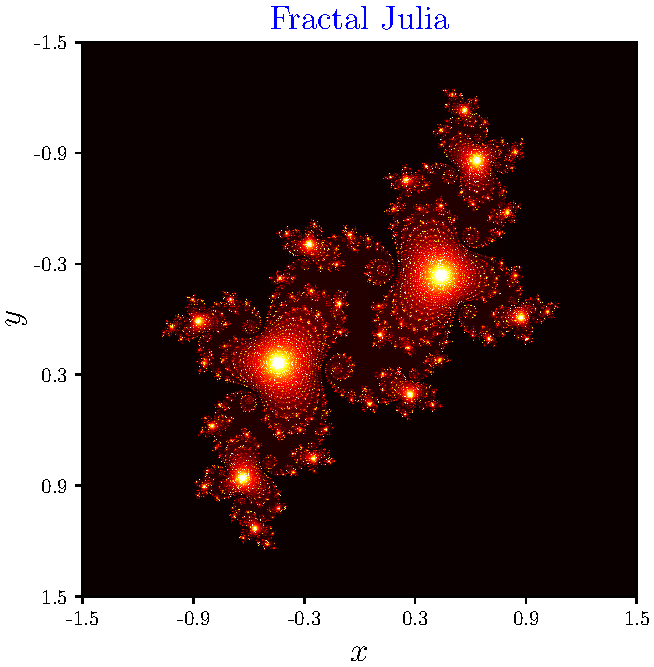
\includegraphics[width=3.0 in]{figuras/complexo/fractal_julia.pdf}
\caption[Fractal Julia.]{Fractal do tipo Julia referente ao Problema \ref{chapseriescomplexos}.\ref{procomfrajulia}. Par�metros utilizados: $f(z) = z^2$, $c=-1+0,65i$, $\Xi = 2000$, $-1,5 < x,y < 1,5$ e $L=10$.}
\label{fractal_julia}
\end{SCfigure} %acertado

\include{arquivos/EDO}

\chapter{Fun��es especiais}  \label{capitulofuncoesespeciais}


\begin{flushright}
\begin{small}
{\color{blue}\textit{
Richard Gervais: There was a time that everything in the universe was once crunched into something smaller than an atom ...

Stephen Colbert: But you dont know that. You're just believing Stephen Hawking and that's a matter of faith in his abilities. You dont know it yourself, you're accepting that because someone told you.

RG: Well, yeah... But science is constantly proved all the time. If we take any fiction book and destroy it, in a thousand years' time that wouldn't come back just as it was. Whereas if we took every science book, every fact, and destroy them all, in a thousand years they'd all be back. Because all the same tests would give the same results.

SC: That's good. That's really good.}}  \\
\textbf{Stephen Colbert show.}
\end{small}
\end{flushright}

\section{Fun��es de Bessel}



Fun��es de Bessel aparecem em uma grande variedade de problemas f�sicos. Por exemplo a parte espacial da equa��o de Helmholtz e da equa��o de onda em coordenadas cil�ndricas leva a fun��es de Bessel como solu��es. J� as mesmas equa��es em coordenadas esf�ricas levam as chamadas fun��es de Bessel esf�ricas. Vibra��es de uma superf�cie analisadas em coordenadas cil�ndricas $R(r)e^{in\varphi}$ leva a fun��es de Bessel para $R(r)$ tendo o inteiro $n$ como par�metro. A aproxima��o WKB, muito utilizada em mec�nica qu�ntica, tamb�m envolve fun��es de Bessel.

Fun��es de Bessel na verdade � um nome gen�rico para um conjunto de fun��es. H� v�rias conven��es diferentes utilizadas tanto para a nota��o quanto para a defini��o de algumas dessas fun��es. Para fins did�ticos vamos adotar aqui a nota��o definida na tabela \ref{funcoesdebessel}.

\begin{table}[h!]
\setlength{\arrayrulewidth}{1.0pt}
\centering
\arrayrulecolor{blue}
\renewcommand{\arraystretch}{2.0}% Spread rows out...
\begin{tabular}{ c | c | c }
\hline \hline
Nome  & Primeiro tipo & Segundo tipo  \\
\hline Fun��o de Bessel &  $J_{\nu}$  & $Y_{\nu}$  \\
\hline Fun��o de Hankel &  $H_{\nu}^{(1)} = J_{\nu} + iY_{\nu}$  & $H_{\nu}^{(2)} = J_{\nu} -i Y_{\nu}$ \\
\hline Fun��o de Bessel modificada &  $I_{\nu}$  & $K_{\nu}$  \\
\hline Fun��o de Bessel esf�rica &  $j_{\nu}$  & $y_{\nu}$  \\
\hline Fun��o de Hankel esf�rica &  $h_{\nu}^{(1)} = j_{\nu} + iy_{\nu}$  & $h_{\nu}^{(2)} = j_{\nu} -i y_{\nu}$ \\
\hline Fun��o de Bessel esf�rica modificada &  $i_{\nu}$  & $k_{\nu}$  \\
\hline
\hline
\end{tabular}
\caption[Fun��es de Bessel]{Nomes dos diversos tipos de fun��es de Bessel. As fun��es da coluna do meio s�o do primeiro tipo e da coluna da direita do segundo tipo. Tamb�m � muito utilizado a nota��o $N_{\nu}$ e  $n_{\nu}$ no lugar de $Y_{\nu}$ e $y_{\nu}$.}
\label{funcoesdebessel}
\end{table}


H� v�rias formas de se encontrar as fun��es de Bessel. Uma delas � a partir da equa��o diferencial
\begin{equation}
x^2 Z_{\nu}'' + x Z_{\nu}' + (x^2 - \nu^2) Z_{\nu} = 0, \label{eqdebesselgenerica}
\end{equation}
onde $\nu$ n�o precisa ser inteiro e $x$ � uma vari�vel admensional\footnote{� comum usar $\nu$ como �ndice n�o inteiro e reservar $n$ para o �ndice inteiro.}. Assim, qualquer fun��o $Z_{\nu}$ que satisfa�a esta equa��o diferencial � chamada de fun��o de Bessel. Se o argumento � $x=kr$ (comum em v�rios problemas de f�sica) a equa��o fica:
\begin{equation}
r^2 \dfrac{d^2}{dr^2} Z_{\nu}(kr) + r \dfrac{d^2}{dr^2}Z_{\nu}(kr) + (k^2r^2 - \nu^2) Z_{\nu}(kr) = 0. \label{skwjwuiedjk}
\end{equation}
Um desses casos � equa��o de Helmholtz $\nabla^2\psi + k^2 \psi = 0$ escrita em coordenadas cil�ndricas, que tamb�m resulta na equa��o acima.


A equa��o diferencial de Bessel � de ordem 2, logo admite duas solu��es LI. A primeira � a fun��o de Bessel $J_n(x)$ e a segunda � chamada de fun��o de Neumann, ou Bessel de segundo tipo:
\begin{equation}
Y_{\nu} = \dfrac{\cos (\nu \pi) J_{\nu} (x) - J_{-\nu} (x) }{\sin \nu \pi}
\end{equation}
Assim, a solu��o geral da equa��o de Bessel �:
\begin{equation}
Z_{\nu}(x) = A J_{\nu} (x) + B Y_{\nu} (x). \label{solbesseprimetipo}
\end{equation}
Na figura \ref{bessel_functions} est� o gr�fico com as primeiras fun��es $J_n$ e $Y_n$.





\begin{tcolorbox}[breakable,pad at break*=1mm,colback=blue!5!white,colframe=DarkGreen!75!black,title=Um pouco de hist�ria.]
  \textbf{Friedrich Wilhelm Bessel}. Astr�nomo alem�o (1784-1846). Com 20 anos de idade, ele refez o c�lculo da �rbita do cometa Halley, o que valeu para ele um posto de trabalho em um observat�rio. Nesta �poca, Bessel desenvolveu as fun��es que leva seu nome em seu trabalho de refirnar c�lculos astron�micos. Bessel fez tamb�m a primeira medida de paralaxe da estrela Cygni 61 (6 anos luz distante de n�s) em 1838, provando de forma definitiva que a Terra est� em movimento de transla��o em torno do Sol, de acordo com a teoria de Nicolau Cop�rnico. Bessel tamb�m calculou as irregularidades da �rbita de Urano, o que contribuiu para a descoberta de Netuno por Leverrier e J. C. Adams, de acordo com a Mec�nica Cl�ssica de Newton.
\end{tcolorbox}


\begin{figure}[!h]
\centering
\subfigure{a)
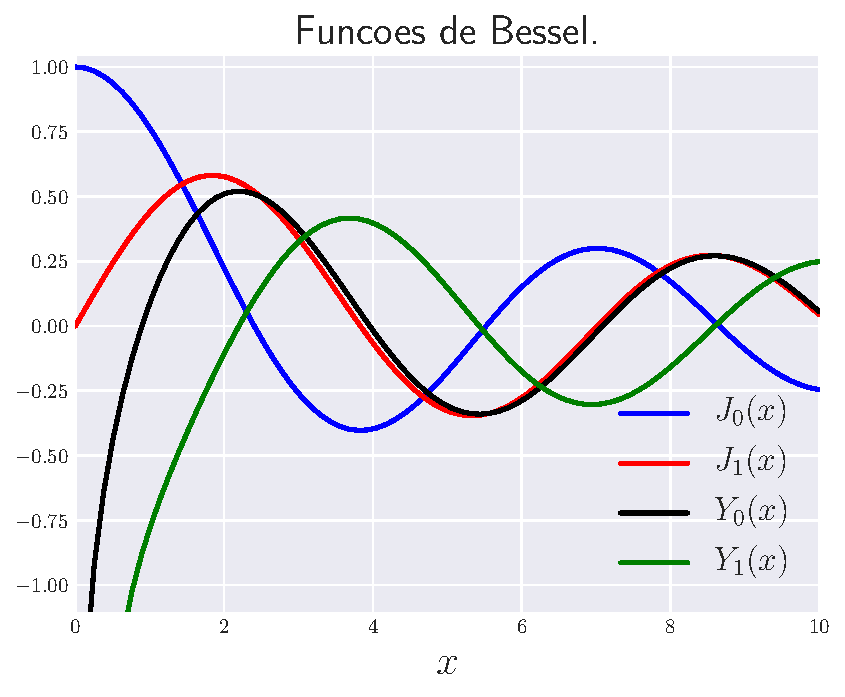
\includegraphics[width = 3.0 in]{figuras/fespeciais/bessel_functions.pdf}
\label{bessel_functions} 
}
\subfigure{b)
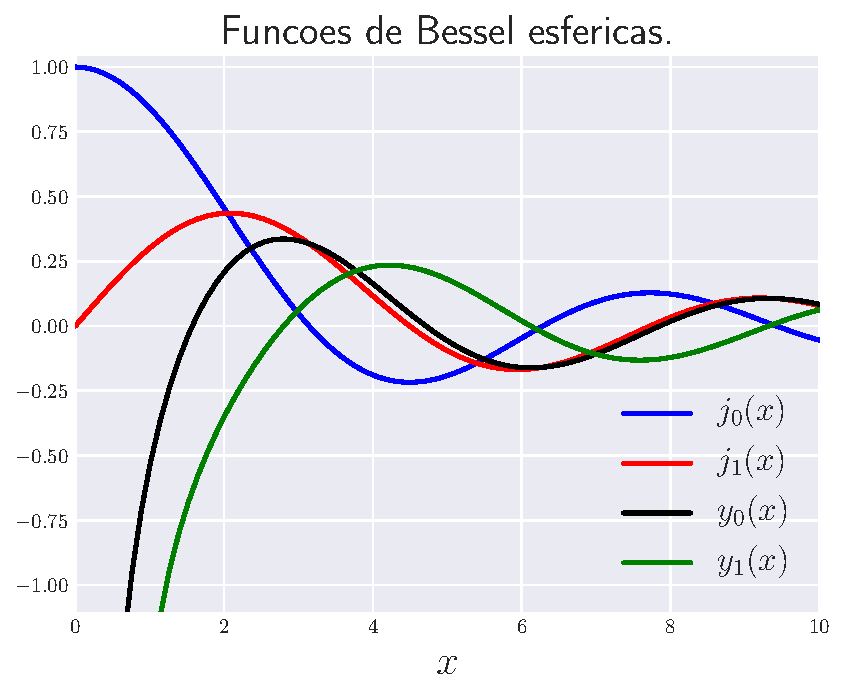
\includegraphics[width = 3.0 in]{figuras/fespeciais/spherical_bessel_functions.pdf}
\label{spherical_bessel_functions}
} 
\caption{\subref{bessel_functions} Fun��es de Bessel $J_n(x)$ e $Y_n(x)$ para $n=1$, 2. \subref{spherical_bessel_functions} Fun��es de Bessel esf�rica $j_n(x)$ e $y_n(x)$ para $n=1$, 2.}
\end{figure}



\subsection{Solu��o em s�rie}

Vamos resolver a Eq. \ref{eqdebesselgenerica} por s�ries usando supondo $y(x) = \sum_{\lambda=0}^{\infty} a_{\lambda} x^{k+\lambda}$. Diferenciando e inserindo $y(x)$ na Eq. \ref{eqdebesselgenerica} temos:
 \begin{equation}
 \sum_{\lambda=0}^{\infty} a_{\lambda} (k+\lambda) (k+\lambda -1) x^{k+\lambda} +  \sum_{\lambda=0}^{\infty} a_{\lambda} (k+\lambda)  x^{k+\lambda} + \sum_{\lambda=0}^{\infty} a_{\lambda}  x^{k+\lambda + 2} - \sum_{\lambda=0}^{\infty} a_{\lambda} n^2 x^{k+\lambda} = 0. \label{eqcoefjslwkejppp}
 \end{equation}
 Resolver uma equa��o diferencial por s�ries consiste em encontrar os coeficientes $a_{\lambda}$ usando a Eq. \ref{eqcoefjslwkejppp}. Quando um polin�mio � igual a zero, todos os seus coeficientes tem que ser zeros. Temos ent�o que analisar todos os termos. Come�amos com o primeiro, que consiste em $\lambda = 0$ (coeficiente de $x^0$). Calculando esse termo e igualando a zero temos:
 \begin{equation}
 a_0 [k(k-1) + k - n^2] = 0. \nonumber
 \end{equation}
 Por�m, assumimos que $a_0 \neq 0$ logo resulta que $k^2 - n^2 = 0$. As solu��es s�o $k = \pm n$.
 
 Agora consideramos o termo $x^{k+1}$ e igualando seu coeficiente a zero obtemos $a_1(k+1-n)(k+1+n) = 0$. Por�m essa equa��o n�o � satisfeita por $k = \pm n$, e temos ent�o de impor $a_1=0$. O pr�ximo termo � $x^{k+\lambda}$ com $\lambda = 2$, depois com $\lambda = 3$, e assim sucessivamente. Fazemos ent�o $\lambda = j$ no primeiro, segundo e quarto termo da Eq. \ref{eqcoefjslwkejppp} e $\lambda = j-2$ no terceiro termo. Fazendo o coeficiente de $x^{k+j}$ igual a zero temos (veja problema \ref{capitulofuncoesespeciais}.\ref{prob1besselssd}):
 \begin{equation}
 a_j [(n+j)(n+j-1)+(n+j)-n^2] + a_{j-2} = 0. \label{coeficeienzeroxkj}
\end{equation}  
A rela��o de recorr�ncia fica ent�o:
\begin{equation}
a_j = -\dfrac{a_j}{(j+2)(2n+j+2)}.  \nonumber
\end{equation}
A rela��o de recorr�ncia � mais �til em fun��o de $a_0$:
\begin{equation}
a_{2p} = (-1)^p \dfrac{a_0 n!}{2^{2p} p! (n+p)!}. \label{relacorecorrenxibessel}
\end{equation}
Agora podemos obter a solu��o, inserindo os coeficientes na solu��o tentativa:
\begin{eqnarray}
y(x) &=& a_0 x^n \left[ 1 - \dfrac{n! x^2}{2^2 1! (n+1)!} + \dfrac{n! x^4}{2^4 2! (n+2)!} + ... \right] , \nonumber \\
&=& a_0 2^n n! \sum_{j=0}^{\infty} \dfrac{(-1)^j}{j! (n+j)!} \left( \dfrac{x}{2} \right)^{n+2j}. \label{sseriefinalbessel} 
\end{eqnarray}
A menos da constante, a s�rie da fun��o de Bessel � escrita como:
\begin{equation}
J_n(x) = \sum_{s=0}^{\infty} \dfrac{(-1)^s}{s! (s+n)!} \left( \dfrac{x}{2} \right)^{n+2s}. \label{sserie2ddfinalbessel} 
\end{equation}

%
%\begin{figure}
%\centering
%\includegraphics[width=4.2 in]{figuras/fespeciais/Bessel_Functions.png}
%\label{Bessel_Functions}
%\caption{Gr�fico das fun��es de Bessel do primeiro tipo $J_n(x)$.}
%\end{figure}


\subsection{Outras fun��es} \label{ssublsjankehkk}

V�rias outras fun��es de Bessel podem ser definidas tamb�m. Por exemplo as fun��es de Hankel est�o definidas na tabela \ref{funcoesdebessel}. A utilidade dessas fun��es reside em suas propriedades assint�ticas, aplicadas por exemplo na propaga��o de ondas esf�ricas ou cil�ndricas. Como $J_{\nu}$ e $Y_{\nu}$ formam um conjunto completo, as fun��es de Hankel n�o podem ser inteiramente novas, por isso elas s�o definidas em fun��o de $J_{\nu}$ e $Y_{\nu}$.



Dessas defini��es pode-se mostrar que:
\begin{eqnarray}
J_{\nu} (z) &=& \dfrac{1}{2} \left[ H_{\nu}^{(1)} (z) + H_{\nu}^{(2)} (z) \right], \nonumber \\ 
Y_{\nu} (z) &=& \dfrac{1}{2i} \left[ H_{\nu}^{(1)} (z) - H_{\nu}^{(2)} (z) \right]. \nonumber
\end{eqnarray}
Temos tamb�m as seguintes propriedades:
\begin{equation}
H_{\nu}^{(1)} (z) = e^{-i\nu \pi} H_{-\nu}^{(1)} (z), \qquad H_{\nu}^{(2)} (z) = e^{i\nu \pi} H_{-\nu}^{(2)} (z). \nonumber
\end{equation}
Usando essas express�es pode-se mostrar que:
\begin{equation}
J_{-\nu} (z) = \dfrac{1}{2} \left[ e^{i\nu \pi} H_{\nu}^{(1)} (z) + e^{-i\nu \pi}H_{\nu}^{(2)} (z) \right]. \label{alskdjfkwiuwppp}
\end{equation}

Tem-se ainda as chamadas fun��o de Bessel modificada. Comecemos com a equa��o de difus�o:
\begin{equation}
\nabla^2\psi - k^2 \psi = 0 \nonumber
\end{equation}
que � muito parecida com a Eq. de Helmholtz. Fazendo o desenvolvimento an�logo ao que levou a Eq. \ref{skwjwuiedjk} teremos:
\begin{equation}
\rho^2 \dfrac{d^2}{	d \rho^2} \Gamma_{\nu} (k\rho) + \rho \dfrac{d}{	d \rho} \Gamma_{\nu} (k\rho) - ( k^2 \rho^2 - \nu^2) \Gamma_{\nu} (k\rho) = 0 \label{eqzzzdkskanllll}
\end{equation}
A diferen�a � que o $+$ antes do par�nteses virou $-$. Na pr�tica, a Eq. de Helmholtz pode ser transformada na Eq. de difus�o fazendo $k\rightarrow ik$, o que tamb�m leva a Eq. \ref{skwjwuiedjk} para a Eq. \ref{eqzzzdkskanllll} de forma que $\Gamma_{\nu} (k\rho) = Z_{\nu} (ik\rho)$ (veja Eq. \ref{solbesseprimetipo}). Ou seja, as solu��es $\Gamma_{\nu} (k\rho)$ s�o fun��es de Bessel com argumento imagin�rio. Por conven��o e conveni�ncia, define-se ent�o:
\begin{equation}
\Gamma_{\nu} (k\rho) = I_{\nu} (x)   \equiv  i^{-\nu} J_{\nu} (ix) \label{definifunImodi}
\end{equation}
onde fizemos $x = k\rho$. Dessa defini��o, podemos escrever as formas: 
\begin{equation}
I_{\nu} (x) = \exp \left( -\frac{1}{2}\nu \pi i \right)   J_{\nu} (xe^{i\pi/2}), \qquad
I_{\nu} (x) = \sum_{s=0}^{\infty} \dfrac{1}{s! (s+\nu)! } \left( \dfrac{x}{2} \right)^{2s+\nu}.  \label{expreIdlkjmodifica}
\end{equation}


%\begin{eqnarray}
%I_{\nu} (x)   = \exp \left( -\frac{1}{2}\nu \pi i \right)   J_{\nu} (xe^{i\pi/2}) \quad &\therefore& \quad  \nonumber  I_{\nu-1} (x)- I_{\nu+1} (x) = \dfrac{2\nu}{x}  I_{\nu} (x)  \\
%I_{\nu} (x) = \sum_{s=0}^{\infty} \dfrac{1}{s! (s+\nu)! } \left( \dfrac{x}{2} \right)^{2s+\nu} \quad &\therefore& \quad I_{-\nu} (x) = \sum_{s=0}^{\infty} \dfrac{1}{s! (s-\nu)! } \left( \dfrac{x}{2} \right)^{2s-\nu}
%\end{eqnarray}


\subsection{Fun��es de Bessel esf�ricas}



Quando a equa��o de Helmholtz � separada em coordenadas esf�ricas a parte radial fica da forma:
\begin{equation}
r^2 \dfrac{d^2R}{dr^2} + 2r \dfrac{dR}{dr}  + \left[  \kappa^2 r^2 - n(n+1) \right] R = 0 \label{edfdfdfdfdfd}
\end{equation}
$n(n+1)$ � uma constante de separa��o. Esta equa��o � semelhante mas n�o � a equa��o de Bessel. Se fizermos a separa��o:
\begin{equation}
R(\kappa r) = \dfrac{Z(\kappa r)}{\sqrt{\kappa r}}   \nonumber
\end{equation}
a Eq. (\ref{edfdfdfdfdfd}) fica:
\begin{equation}
r^2 \dfrac{d^2Z}{dr^2} + 2r \dfrac{dZ}{dr}  + \left[  \kappa^2 r^2 - \left( n+\frac{1}{2}\right)^2  \right] Z = 0   \label{lkjjhyuuioo}
\end{equation}
que � a equa��o de Bessel para $Z$ de ordem $n+\frac{1}{2}$ de forma que $Z(\kappa r) =J_{n+\frac{1}{2}} (\kappa r)$. Assim, formalmente, $Z(\kappa r)$ ser� uma combina��o linear entre $J_{n+\frac{1}{2}}$ e $Y_{n+\frac{1}{2}}$. 
\begin{equation}
G(r) = Aj_n(\kappa r) + By_n(\kappa r) \label{soleqbesseesferica}
\end{equation}
as quais s�o definidas da seguinte forma:
\begin{equation}
j_n(x) = \sqrt{\dfrac{\pi}{2x}} J_{n+1/2} (x),  \qquad \qquad y_n(x) = \sqrt{\dfrac{\pi}{2x}} Y_{n+1/2} (x)   = (-1)^{n+1} \sqrt{\dfrac{\pi}{2x}} J_{-n-1/2} (x) \nonumber
\end{equation}
onde $n$ � um inteiro. Na figura \ref{spherical_bessel_functions} est� o gr�fico com as primeiras fun��es $j_n$ e $y_n$. Al�m disso, as fun��o de Haenkel esf�ricas s�o definidas como:
\begin{eqnarray}
h_n^{(1)} &=& \sqrt{\dfrac{\pi}{2x}} H_{n+1/2}^{(1)} (x) = j_n(x) + i y_n(x), \nonumber \\
h_n^{(2)} &=& \sqrt{\dfrac{\pi}{2x}} H_{n+1/2}^{(2)} (x) = j_n(x) - i y_n(x). \nonumber
\end{eqnarray}

Trabalhando as rela��es de recorr�ncias e express�o em s�rie de $J_n$ e $Y_n$, pode-se mostrar que as express�es em s�rie de $j_n$ e $y_n$ s�o:
\begin{eqnarray}
j_n(x) &=& 2^n x^n \sum_{s=0}^{\infty} \dfrac{(-1)^s (s+n)!}{s! (2s+2n+1)} x^{2s}, \nonumber \\
y_n(x) &=& \dfrac{(-1)^{n+1}}{2^n x^{n+1}} \sum_{s=0}^{\infty} \dfrac{(-1)^s (s-n)!}{s! (2s-2n)} x^{2s}. \nonumber 
\end{eqnarray}

J� as rela��es de recorr�ncia s�o:
\begin{eqnarray}
\dfrac{d}{dx} \left[ x^{n+1} f_n(x) \right] &=& x^{n+1} f_{n-1}(x), \nonumber \\
\dfrac{d}{dx} \left[ x^{-n} f_n(x) \right] &=& -x^{-n} f_{n+1}(x), \nonumber 
\end{eqnarray}
onde $f_n$ pode ser $j_n$, $y_n$, $h_n^{(1)}$ e $h_n^{(2)}$. Usando essas rela��es, pode-se provar por indu��o matem�tica que:
\begin{eqnarray}
j_n(x) &=& (-1)^n x^n \left( \dfrac{1}{x} \dfrac{d}{dx} \right)^n \left( \dfrac{\sin x}{x}\right), \label{proindjnslkj} \\  
y_n(x) &=& -(-1)^n x^n \left( \dfrac{1}{x} \dfrac{d}{dx} \right)^n \left( \dfrac{\cos x}{x}\right), \label{prssndynslkj} \\  
h_n^{(1)}(x) &=& -i(-1)^n x^n \left( \dfrac{1}{x} \dfrac{d}{dx} \right)^n \left( \dfrac{e^{ix}}{x}\right), \label{pkskndh1nslkj} \\  
h_n^{(2)}(x) &=& i(-1)^n x^n \left( \dfrac{1}{x} \dfrac{d}{dx} \right)^n \left( \dfrac{e^{-ix}}{x}\right). \label{pkndh2nslkj}   
\end{eqnarray}

\begin{exemplo} \label{exeesfeparconfiinfin}
\textbf{Part�cula em uma esfera}. Vamos considerar a descri��o qu�ntica de uma part�cula confinada em uma esfera de raio $a$. O potencial que a esfera sente �:
\begin{equation}
V(r) = \left\{
\begin{array}{rl}
0 & \text{se } r \leq a  \\
\\
 \infty& \text{se } r > a
\end{array} 
 \right. \nonumber
\end{equation}
As condi��es de contorno s�o: (i) $\psi ( r\leq a)$ deve ser finito e (ii) $\psi (a) = 0$. Encontre o valor m�nimo da energia $E$ para o qual h� uma solu��o v�lida da Eq. de Schrodinger.
\tcblower
Como o potencial s� depende da coordenada esf�rica $r$, podemos desprezar a depend�ncia angular. Esta part�cula deve obedecer a Eq. de Schrodinger\footnote{$\hbar = h/(2\pi)$ e $m$ � a massa da part�cula.} independente do tempo. Para $r \leq a$ temos:
\begin{equation}
-\dfrac{\hbar^2}{2m} \nabla^2 \psi = E \psi, \label{eqschrodparesferinfinito}
\end{equation}
logo
\begin{equation}
\dfrac{d^2R}{dr^2} + \dfrac{2}{3} \dfrac{dR}{dr} + \left[ k^2 - \dfrac{n(n+1)}{r^2} \right] R = 0, \nonumber
\end{equation}
onde $k^2 = 2mE/\hbar^2$. Veja que essa equa��o � id�ntica a Eq. \ref{edfdfdfdfdfd} cujas solu��es s�o da forma da Eq. \ref{soleqbesseesferica}. Por�m, como queremos o valor m�nimo de energia vamos usar $n=0$ de forma que a solu��o para nosso problema �:
\begin{equation}
R(r) = Aj_0 (kr) + B y_0 (kr). \label{solbessesfepocoinfi}
\end{equation}
Por�m, na origem a fun��o $y_n$ diverge, ent�o ela deve ser descartada. Para satisfazer a condi��o de contorno (ii) temos que $j_0(ka)=0$. Isto limita os valores poss�veis de $k$, consequentemente, os valores de energia $E$ tamb�m ficam limitados a valores discretos. Ou seja, a energia � quantizada. O menor valor para os zeros de $j_0$ � $\pi$, logo $k_1a=\pi$ o que implica:
\begin{equation}
E_1 = \dfrac{h^2}{8ma^2}, \nonumber
\end{equation}
como sendo o menor valor poss�vel para a energia. Veja que o resultado � semelhante a energia m�nima de uma part�cula confinada em uma caixa retangular de lados $a$, $b$ e $c$: $E_1 = (h^2/8m)(1/a^2+1/b^2+1/c^2)$.
\end{exemplo}


\subsubsection{Fun��es de Bessel esf�ricas modificadas}


Da mesma forma que existem as fun��es de Bessel modificadas $I_{\nu}$ e $K_{\nu}$ (veja problema \ref{capitulofuncoesespeciais}.\ref{profunbessmodisegun}), existem tamb�m as fun��es de Bessel esf�ricas modificadas $i_{\nu}$ e $k_{\nu}$. A equa��o diferencial que as definem �:
\begin{equation}
r^2 \dfrac{d^2R}{dr^2} + 2r \dfrac{dR}{dr}  - \left[  \kappa^2 r^2 + n(n+1) \right] R = 0 \label{edf22222fdfd}
\end{equation}
Repare que esta equa��o difere da Eq. \ref{edfdfdfdfdfd} apenas pelo sinal de $\kappa^2 r^2$. Seguindo a analogia, as solu��es desta equa��o s�o definidas como:
\begin{equation}
i_n(x) = \sqrt{\dfrac{\pi}{2x}} I_{n+1/2} (x),  \qquad \qquad k_n(x) = \sqrt{\dfrac{\pi}{2x}} K_{n+1/2} (x) \nonumber
\end{equation}




{\noindent\def\stackalignment{l}% code from https://tex.stackexchange.com/a/195118/101651
    \stackunder[0pt]{\colorbox{cyan}{\textcolor{white}{\textbf{\LARGE Problemas}}}}{\textcolor{lightcyan}{\rule{\linewidth}{2pt}}}\medskip}
    


\begin{problema} \label{prob1besselssd}
a) Obtenha a Eq. \ref{coeficeienzeroxkj}. b) Obtenha a rela��o de recorr�ncia \ref{relacorecorrenxibessel}. c) Obtenha a express�o final da s�rie \ref{sseriefinalbessel}.
\end{problema}


\begin{problema}
Mostre as seguintes rela��es de recorr�ncia:
\begin{equation}
\dfrac{d}{dx} \left[ x^{-n} J_n(x) \right] = -x^{-n} J_{n+1} (x), \qquad \qquad \dfrac{n}{x}J_n(x) - J_{n+1}(x) = J_n'(x). \nonumber
\end{equation}
Dica: fa�a $s \rightarrow s-1$ na Eq. \ref{sserie2ddfinalbessel} para $J_{n+1}(x)$.
\end{problema}

\begin{problema}
Mostre que a) $Y_{-n} (x) = (-1)^n Y_n(x)$ e b) $Y_0'(x) = -Y_1(x)$.
\end{problema}


\begin{problema}
Mostre que em coordenadas cil�ndricas, a Eq. de Helmholtz $\nabla^2\psi + k^2 \psi = 0$ se reduz a equa��o de Bessel. A Eq. de Helmholtz � a parte espacial da equa��o de onda.
\end{problema}

\begin{problema}
a) Obtenha a Eq. \ref{eqzzzdkskanllll} a partir da Eq. de difus�o. b) Mostre que esta equa��o pode ser obtida fazendo $k\rightarrow ik$ na Eq. de Helmholtz.
\end{problema}

\begin{problema}
a) Mostre que as express�es da Eq. \ref{expreIdlkjmodifica} s�o compat�veis com a defini��o da Eq. \ref{definifunImodi}.
b) Mostre tamb�m que:
\begin{equation}
 I_{-\nu} (x) = \sum_{s=0}^{\infty} \dfrac{1}{s! (s-\nu)! } \left( \dfrac{x}{2} \right)^{2s-\nu}
\end{equation}
\end{problema}

\begin{problema} \label{profunbessmodisegun}
A Eq. \ref{eqzzzdkskanllll} � de segunda ordem e aceita uma segunda solu��o independente al�m de $I_{\nu}(x)$. A flexibilidade � grande e assim a defini��o dessa fun��o � uma quest�o de conveni�ncia. Uma forma de se definir �:
\begin{equation}
K_{\nu}(x) \equiv \dfrac{\pi}{2} i^{\nu+1} H_{\nu}^{(1)} (ix) = \dfrac{\pi}{2} i^{\nu+1} \left[ J_{\nu} (ix) + i N_{\nu} (ix) \right]. \nonumber 
\end{equation}
$I_{\nu}(x)$ e $K_{\nu}(x)$ s�o as fun��es de Bessel modificadas do primeiro e segundo tipo. a) Mostre que $K_{\nu}(x)$ � real se $x$ for real. b) Mostre que pode-se escrever tamb�m:
\begin{equation}
K_{\nu}(x) = \dfrac{\pi}{2} \dfrac{I_{-\nu}(x)-I_{\nu}(x)}{\sin (\nu \pi)}. \nonumber
\end{equation}
\end{problema}

\begin{problema} \label{rprofunbessesfern0e1}
Calcule as fun��es de Bess esf�ricas $j_n$ $y_n$, $h^{(1)}$ e $h^{(2)}$ para $n=$ 0 e 1.
\end{problema}

\begin{problema}
$\bigstar$ Mostre que:
\begin{eqnarray}
\cos x &=& J_0(x) + 2\sum_{n=1}^{\infty} (-1)^n J_{2n} (x), \nonumber \\
\sin x &=&  2\sum_{n=1}^{\infty} (-1)^{n+1} J_{2n+1} (x). \nonumber
\end{eqnarray}
\end{problema}

\begin{problema}
$\bigstar$ Deduza a Eq. \ref{proindjnslkj}. b) Deduza a Eq. \ref{prssndynslkj}.
\end{problema}


\begin{problema}
$\bigstar$ Deduza a Eq. \ref{pkskndh1nslkj}. b) Deduza a Eq. \ref{pkndh2nslkj}.
\end{problema}

\begin{problema}
$\bigstar$ Deduza a Eq. \ref{alskdjfkwiuwppp}.
\end{problema}




\begin{problema}
$\bigstar$ Deduza a rela��o de completeza da fun��o de Bessel esf�rica:
\begin{equation}
\int_0^{+\infty} j_n(ar) j_n(br) r^2 dr = \dfrac{\pi}{2a^2} \delta (a-b). \nonumber
\end{equation}
Dica: P. Ugincius, \textit{Am. J. Phys.} 40, 1690 (1972).
\end{problema}


\begin{problema}
\textbf{Fun��es de Bessel esf�ricas modificadas}.Mostre que $i_n(x)$ e $k_n(x)$ satisfazem a Eq. \ref{edf22222fdfd}.
\end{problema}

\begin{problema}
Deduza as seguintes rela��es de recorr�ncia:
\begin{eqnarray}
i_{n-1}(x) - i_{n+1}(x) = \dfrac{2n+1}{x}i_n(x) \quad &\therefore&  \quad k_{n-1}(x) - k_{n+1}(x) = -\dfrac{2n+1}{x}k_n(x) \nonumber \\
\dfrac{d}{dx} i_n(x) &=& \dfrac{1}{2n+1} \left[  ni_{n-1}(x) +(n+1)i_{n+1}(x) \right]  \nonumber  \\
\dfrac{d}{dx} k_n(x) &=& -\dfrac{1}{2n+1} \left[  nk_{n-1}(x) +(n+1)k_{n+1}(x) \right]  \nonumber  
\end{eqnarray}
\end{problema}


\begin{problema}
$\bigstar \bigstar$ Uma fun��o $\mathscr{H}$ � chamada de cil�ndrica quando ela satisfaz as seguintes propriedades:
\begin{eqnarray}
\mathscr{H}_{\nu -1} (z) + \mathscr{H}_{\nu +1} (z) &=& \dfrac{2\nu}{z}  \mathscr{H} (z), \nonumber \\
\mathscr{H}_{\nu -1} (z) - \mathscr{H}_{\nu +1} (z) &=& 2\dfrac{d\mathscr{H}}{dz}. \nonumber
\end{eqnarray}
onde $\nu$ e $z$ s�o n�meros complexos. Prove que as fun��es de Bessel $J_n$, $Y_n$, $H_n^{(1)}$, $H_n^{(2)}$ s�o fun��es cil�ndricas\footnote{Dica: G. N. Watson \textit{A Treatise on the Theory of the Bessel Functions}, Cambridge University Press (1944), p�g. 82.}.
\end{problema}

\begin{problema}
$\bigstar \bigstar$ Seja:
\begin{equation}
\int z^{\nu + 1} f(z) \mathscr{M}_{\nu} (z) dz = z^{\nu + 1} \left[ A(z) \mathscr{M}_{\nu} (z) + B(z) \mathscr{M}_{\nu+1} (z) \right], \nonumber
\end{equation}
onde $A(z)$ e $B(z)$ s�o coeficientes e $\mathscr{M}_{\nu} (z)$ � uma fun��o cil�ndrica, ou seja, pode ser $J_n$, $Y_n$, $H_n^{(1)}$, $H_n^{(2)}$ ou uma combina��o linear dessas fun��es. Mostre que\footnote{Dica: G. N. Watson \textit{A Treatise on the Theory of the Bessel Functions}, Cambridge University Press (1944), p�g. 132. Este resultado foi obtido primeiramente em 1868.}
\begin{equation}
f(z) = B''(z) + \dfrac{2\nu + 1}{z} B'(z) + B(z). \nonumber 
\end{equation}
\end{problema}



{\noindent\def\stackalignment{l}{\textcolor{lightcyan}{\rule{\linewidth}{2pt}}}\medskip}


\section{Polin�mios de Legendre}

Polin�mios de Legendre s�o fun��es que aparecem em diversos problemas de f�sica, por exemplo, nos harm�nios esf�ricos e expans�o do potencial el�trico e gravitacional e satisfazem a seguinte equa��o diferencial:
\begin{equation}
\dfrac{d}{dx} \left[ (1-x^2) \dfrac{dP}{dx} \right] + n(n+1)P = 0. \label{eqdiferedefinpolilegendre}
\end{equation}
Em f�sica, � comum encontrar esta equa��o em termos de $\theta$, sendo $x = \cos \theta$. Nesta forma temos:
\begin{equation}
\dfrac{1}{\sin \theta}\dfrac{d}{d\theta} \left[ \sin \theta \dfrac{dP}{d\theta} \right] + n(n+1)P = 0. \nonumber
\end{equation}
As solu��es dessa equa��o podem ser encontradas de diversas formas. Uma delas � atrav�s da f�rmula de Rodrigues\footnote{O fator $\dfrac{1}{2^l l!}$ foi escolhido para que $P_l(1) = 1$.}:
\begin{equation}
P_l(x) = \dfrac{1}{2^l l!} \left( \dfrac{d}{dx} \right)^l (x^2 - 1)^l. \label{polinolegendrodires}
\end{equation}
Veja que $P_l(x)$ � um polin�mio de ordem $l$ em $x$ no qual $l$ � um inteiro n�o negativo (inclui o zero). Os primeiros polin�mios de Legendre s�o:
\begin{eqnarray}
P_0 = 1, \qquad \qquad P_1 = x, \qquad \qquad P_2 = \frac{1}{2}(3x^2 - 1), \label{pripolilegensr} \\
P_3 = \frac{1}{2} ( 5x^3 - 3x), \qquad \qquad P_4 = \frac{1}{8} ( 35x^4 - 30x + 3). \nonumber
\end{eqnarray}

Outra forma de encontrar esses polin�mios � usar a fun��o geradora:
\begin{equation}
\Phi(x,h) = \dfrac{1}{\sqrt{1-2xh + h^2}}, \qquad \vert h \vert < 1. \label{funcaogeradorporllegende}
\end{equation}
A propriedade importante dessa fun��o � que:
\begin{equation}
\Phi(x,h) = P_0(x) +hP_1(x) + h^2P_2(x)+ \cdot \cdot \cdot = \sum_{l=0}^{\infty} h^l P_l(x). \label{fungerapolegenepxpans}
\end{equation}
A prova de que os $P_l$ dessa equa��o s�o de fato os polin�mios de Legendre envolve duas coisas: 1) mostrar que $P_l(1)=1$ e que esses $P_l$ satisfazem a equa��o de Legendre. 

A fun��o geradora � muito �til na obte��o de rela��es de recorr�ncia. Alguns exemplos s�o:
\begin{eqnarray}
lP_l(x) &=& (2l-1)xP_{l-1}(x) - (l-1)P_{l-2}(x), \nonumber \\
lP_l(x) &=& xP_l'(x) - P_{l-1}'(x), \label{relrecorenciaPlegen} \\
lP_{l-1}(x) &=& P_l'(x) -x P_{l-1}'(x). \nonumber
\end{eqnarray}

\subsection{Potencial eletrost�tico}

Uma das aplica��es de Polin�mios de Legendre � na aproxima��o do potencial Coulombiano gerado por uma distribui��o de cargas el�trica. Consideremos a figura que mostra uma distribui��o arbitr�ria onde cada elemento de carga � indicado pelo vetor $\textbf{r}'$. Queremos calcular o potencial na posi��o $\textbf{r}$ no caso em que $r << r'$, ou seja, quando queremos o potencial muito longe da distribui��o de carga\footnote{Mas n�o muito longe onde o potencial � zero.}. Esta aproxima��o � amplamente aplicada em situa��es onde a distribui��o de carga ocupa um pequeno volume.

O potencial de uma distribui��o de cargas $\rho$ �:
\begin{equation}
V(\textbf{r}) = \dfrac{1}{4\pi \epsilon_0} \int \dfrac{1}{\rcurs} \rho(\textbf{r}') d\tau', \nonumber
\end{equation}
onde $\brcurs = \textbf{r} - \textbf{r}'$ � vetor separa��o e $r'$ � a vari�vel de integra��o. Da lei dos cossenos:
\begin{equation}
\rcurs = r^2 + (r')^2 - 2rr' \cos \theta = r^2 \left[ 1 + \left( \dfrac{r'}{r} \right)^2 - 2 \left( \dfrac{r'}{r} \right) \cos \theta \right], \nonumber  
\end{equation}
onde $\theta$ � o �ngulo entre $\textbf{r}$ e $\textbf{r}'$. Dado a aproxima��o que estamos fazendo podemos escrever
\begin{equation}
\rcurs = r \sqrt{1 + \varepsilon}, \qquad \varepsilon =  \left( \dfrac{r'}{r} \right) \left( \dfrac{r'}{r} - 2 \cos \theta \right). \nonumber
\end{equation}
Assim, quando $r>>r'$ temos $\varepsilon << 1$. Usando a expans�o binomial:
\begin{equation}
\dfrac{1}{\rcurs} = \dfrac{1}{r \sqrt{1+ \varepsilon}} = \dfrac{1}{r} \left( 1 - \dfrac{1}{2}\varepsilon + \dfrac{3}{8}\varepsilon^2 - \dfrac{5}{16}\varepsilon^3 + \cdot \cdot \cdot \right). \nonumber  
\end{equation}
Substituindo de volta a express�o de $\varepsilon$:
\begin{eqnarray}
\dfrac{1}{\rcurs} &=& \dfrac{1}{r} \left[ 1 - \dfrac{1}{2} \left( \dfrac{r'}{r} \right) \left( \dfrac{r'}{r} - 2 \cos \theta \right) +\dfrac{3}{8} \left( \dfrac{r'}{r} \right)^2 \left( \dfrac{r'}{r} - 2 \cos \theta \right)^2 - \dfrac{5}{16} \left( \dfrac{r'}{r} \right)^3 \left( \dfrac{r'}{r} - 2 \cos \theta \right)^3 \cdot \cdot \cdot \right], \nonumber \\
&=&  \dfrac{1}{r} \left[ 1 + \left( \dfrac{r'}{r} \right) \cos \theta + \left( \dfrac{r'}{r} \right)^2 \left( \dfrac{3\cos^2 \theta - 1}{2} \right) + \left( \dfrac{r'}{r} \right)^3 \left( \dfrac{5\cos^3 \theta - 3\cos \theta}{2} \right) + \cdot \cdot \cdot \right]. \nonumber
\end{eqnarray}
Analisando os coeficientes na �ltima express�o vemos que eles s�o na verdade os Polin�mios de Legendre:
\begin{equation}
\dfrac{1}{\rcurs} = \dfrac{1}{r} \sum_{n=0}^{\infty} \left( \dfrac{r'}{r} \right)^n P_n(\cos \theta). \nonumber
\end{equation} 
Agora podemos montar a express�o final para o potencial:
\begin{equation}
V(\textbf{r}) = \dfrac{1}{4\pi \epsilon_0} \sum_{n=0}^{\infty} \dfrac{1}{r^{n+1}} \int (r')^n P_n(\cos \theta) \rho (\textbf{r}') d\tau'. \nonumber
\end{equation}
Veja que $r$ sai da integral pois n�o depende de $r'$. Esta express�o para o potencial � conhecida como expans�o multipolar. O primeiro termo $n=0$ � a contribui��o do monopolo (decai com $1/r$). O segundo termo $n=1$ � o dipolo, o terceiro $n=3$ � o quadrupolo, o quarto o octopolo, e assim sucessivamente. Esta expans�o � exata (somat�rio at� o infinito) por�m sua utilidade pr�tica est� em considerar apenas alguns termos, suficiente para que o resultado seja dentro do desejado.



\subsection{Polin�mios associados de Legendre}

Uma outra fun��o que tamb�m aparece em f�sica � a solu��o da equa��o diferencial
\begin{equation}
(1-x^2) y'' - 2xy' + \left[ l(l+1) - \dfrac{m^2}{1-x^2} \right] y = 0 \label{eqdiferpoliassoclegend}
\end{equation}
que pode ser escrita como:
\begin{equation}
P_l^m (x) = (1-x^2)^{m/2} \dfrac{d^m}{dx^m} P_l(x). \label{defipoliassocilegendr}
\end{equation} 
Assim, as fun��es $P_l^m (x)$ receberam o nome de polin�mios associados de Legendre.

\begin{SCfigure}
 \centering
\includegraphics[width=3.0 in]{figuras/fespeciais/potencial_expansao.png}
\caption{Potencial de uma carga pontual calculada em uma posi��o arbitr�ria.}
\label{potencial_expansao}
\end{SCfigure} 


{\noindent\def\stackalignment{l}% code from https://tex.stackexchange.com/a/195118/101651
    \stackunder[0pt]{\colorbox{cyan}{\textcolor{white}{\textbf{\LARGE Problemas}}}}{\textcolor{lightcyan}{\rule{\linewidth}{2pt}}}\medskip}
    


\begin{problema} 
a) Mostre que no caso geral 3D, considerando $r_1>r_2$ e usando a Lei dos cossenos, podemos escrever:
\begin{equation}
\dfrac{1}{\vert \textbf{r}_1 - \textbf{r}_2 \vert}  = \dfrac{1}{r_1} \left[ 1 + \left( \dfrac{r_2}{r_1} \right)^2 - 2\left( \dfrac{r_2}{r_1} \right) \cos \theta \right]^{-1/2}. \nonumber  
\end{equation}
Dica: coloque em evid�ncia $r_1 = \vert \textbf{r}_1 \vert$.
b) Usando a fun��o geradora $g(t,x)$, mostre que:
\begin{equation}
\dfrac{1}{\vert \textbf{r}_1 - \textbf{r}_2 \vert}  = \dfrac{1}{r_1} \sum_{n=0}^{+\infty} P_n(\cos \theta) \left( \dfrac{r_2}{r_1} \right)^n . \nonumber  
\end{equation}
\end{problema}

\begin{problema}
a) Seja uma fun��o expandida em polin�mios de Legendre: $f(x) = \sum a_n P_n(x)$. Mostre que:
\begin{equation}
\int_{-1}^{+1} \left[ f(x) \right]^2 dx = \sum_{n=0}^{+\infty} \dfrac{2a_n^2}{2n+1}. \nonumber 
\end{equation}
b) Seja $f(x) = \arcsin x$. Calcule os coeficientes $a_n$ da expans�o.
\end{problema}

\begin{problema}
Considerando $r>n$, mostre que:
\begin{equation}
\int_{-1}^{+1} x^{2r} P_{2n}(x) dx = \dfrac{2^{2n+1} (2r)!(r+n!)}{(2r+2n+1)!(r-n)!}. \nonumber
\end{equation}
\end{problema}


\begin{problema}
Considere $\alpha=2xh -h^2$ na fun��o geradora $\Phi(x,h)$ da Eq. \ref{funcaogeradorporllegende}. Expanda $(1-\alpha)^{-1/2}$ em pot�ncias de $\alpha$ e depois substitua de volta $\alpha=2xh -h^2$. Dessa forma, recupere os primeiros termos da expans�o da Eq. \ref{fungerapolegenepxpans}.
 \end{problema}
 
 
 \begin{problema}
 Uma esfera de raio $R$ centrada na origem possui uma densidade de carga el�trica dada por:
 \begin{equation}
 \rho(r,\theta) = k \dfrac{R}{r^2} (R-3r) \cos \theta,
 \end{equation}
 onde $k$ � uma constante. Encontre o primeiro termo diferente de zero da expans�o multipolar para o potencial ao longo do eixo $z$.
 \end{problema}



\begin{problema}
Usando $x = \cos \theta$ mostre que a Eq. \ref{eqdiferpoliassoclegend} pode ser escrita como:
\begin{equation}
\dfrac{1}{\sin \theta} \dfrac{d}{d \theta} \left( \sin \theta \dfrac{dy}{d \theta} \right) + \left[ l(l+1) - \dfrac{m^2}{\sin^2 \theta} \right] y = 0. \nonumber
\end{equation}
\end{problema}


\begin{problema}
Mostre que a Eq. \ref{defipoliassocilegendr} pode ser escrita como:
\begin{equation}
P_l^m (x) = \dfrac{(1-x^2)^{m/2}}{2^l l!} \dfrac{d^{l+m}}{dx^{l+m}} (x^2-1)^l.
\end{equation}
Dica: use a f�rmula de Rodrigues.
\end{problema}



{\noindent\def\stackalignment{l}{\textcolor{lightcyan}{\rule{\linewidth}{2pt}}}\medskip}


\section{Conjunto completo}

Dois vetores s�o ditos ortogonais se um � perpendicular ao outro: $\textbf{A} \cdot \textbf{B} = 0$. Em um espa�o de $n$ dimens�es essa equa��o fica\footnote{Usamos $x_1=x$, $x_2=y$, $x_3=z$, $x_4=w$, ...} $\sum_i^n A_i B_i = 0$. Esse mesmo conceito de ortogonalidade pode ser aplicado para fun��es onde o somat�rio � trocado por uma integral e o n�mero de dimens�es se converte em um intervalo. A defini��o �: duas fun��es $A(x)$ e $B(x)$ s�o ortogonais em um intervalo $(a,b)$ se
\begin{equation}
\int_a^b A^*(x) B(x) dx = 0, \nonumber
\end{equation}
onde $A^*$ � o complexo conjugado de $A$. No caso de fun��es reais o complexo conjugado � a pr�pria fun��o.

Suponha agora que tenhamos um conjunto de fun��es $A_n(x)$ com $n=1,2,3,...$. Esse conjunto ser� ortogonal se:
\begin{equation}
\int_a^b A_n^*(x) A_m(x) dx = \left\{
\begin{array}{rl}
 0& \text{se  } n \neq m  \\
\\
 C & \text{se  } n = m
\end{array} 
\right. \nonumber
\end{equation}
onde $C \neq 0$ � uma constante diferente de zero. No caso de $C=1$ temos que o conjunto � normalizado, al�m de ser ortogonal. Nesse caso � chamado de conjunto ortogonal. Essa constante � exatamente a constante de normaliza��o j� que a fun��o definida como $B(x) = A(x)/C$ ter� m�dulo 1. Veja que essa defini��o segue a analogia com o caso de vetores onde o m�dulo � $A^2 = \textbf{A} \cdot \textbf{A}$.



\subsection{Polin�mios de Legendre}


Os polin�mios de Legendre formam um conjunto ortogonal. Para construir a rela��o de ortogonalidade vamos primeiro mostrar que a integral em diferentes polin�mios � zero. Escrevemos a Eq. \ref{eqdiferedefinpolilegendre} para $P_n$ e multiplicamos por $P_m$. Depois fazemos o contr�rio: escrevemos a mesma equa��o para $P_m$ e multiplicamos por $P_n$. Por fim subtraimos uma da outra:
\begin{equation}
P_m \dfrac{d}{dx} \left[ (1-x^2)P_n' \right] -P_n \dfrac{d}{dx} \left[ (1-x^2)P_m' \right] + \left[ n(n+1)-m(m+1)\right] P_nP_m=0. \label{wowiwuwjwnmmzzzzz}
\end{equation}
Os dois primeiros termos s�o na verdade a derivada de um termo s�, logo:
\begin{equation}
 \dfrac{d}{dx} \left[ (1-x^2) (P_m P_n' - P_nP_m') \right] + \left[ n(n+1)-m(m+1)\right] P_nP_m=0. \nonumber
\end{equation}
Integrando de -1 a 1:
\begin{equation}
 (1-x^2) (P_m P_n' - P_nP_m')\bigg\rvert_{-1}^1  + \left[ n(n+1)-m(m+1)\right] \int_{-1}^1 P_nP_m=0. \nonumber
\end{equation}
Por�m temos que $1-x^2=0$ para $x=\pm 1$, o que zera o termo da esquerda. Sobra s� o termo da direita. Mas $n(n+1)-m(m+1)  \neq 0$ se $n \neq m$. Logo neste caso a integral deve ser zero:
\begin{equation}
 \int_{-1}^1 P_nP_m=0, \qquad n \neq m. \label{ortognoaPlegend}
\end{equation}
Este resultado mostra que $P_n$ forma um conjunto ortogonal.

Agora precisamos calcular o m�dulo de $P_l$, que � o resultado da integral de superposi��o quando $n=m$. Multiplicando a rela��o de recorr�ncia da Eq. \ref{relrecorenciaPlegen} por $P_l(x)$ e integrando temos:
\begin{equation}
l\int_{-1}^1 \left[ P_l(x) \right]^2 dx =  \int_{-1}^1 x P_l(x) P_l'(x) dx - \int_{-1}^1 P_l(x) P_{l-1}'(x) dx. \label{sskwjwnwmmmmpp} 
\end{equation} 
A �ltima integral � zero (dica: Eq. \ref{ortognoaPlegend}) e a integral do meio pode ser efetuada por partes:
\begin{equation}
\int_{-1}^1 x P_l(x) P_l'(x) dx  = \dfrac{x}{2} \left[ P_l(x) \right]^2\bigg\rvert_{-1}^1 - \frac{1}{2} \int_{-1}^1 \left[ P_l(x) \right]^2 dx = 1 - \frac{1}{2} \int_{-1}^1 \left[ P_l(x) \right]^2 dx. \nonumber 
\end{equation} 
Substituindo esse resultado de volta na Eq. \ref{sskwjwnwmmmmpp} e isolando a integral temos que:
\begin{equation}
\int_{-1}^1 \left[ P_l(x) \right]^2 dx = \dfrac{2}{2l+1}. \nonumber
\end{equation}
Agora podemos montar a rela��o final de ortogonalidade dos polin�mios de Legendre:
\begin{equation}
 \int_{-1}^1 P_n (x) P_m  (x) dx  = \left\{
\begin{array}{rl}
 0& \text{se  } n \neq m  \\
\\
 \dfrac{2}{2n+1}& \text{se  } n = m
\end{array} 
\right. \nonumber
\end{equation}
� muito utilizado em f�sica $P_n(x)$ com $x = \cos \theta$. Neste caso:
\begin{equation}
 \int_0^{\pi} P_n  (\cos \theta ) P_m  (\cos \theta ) \sin \theta d\theta  = \left\{
\begin{array}{rl}
 0& \text{se  } n \neq m  \\
\\
 \dfrac{2}{2n+1}& \text{se  } n = m
\end{array} 
\right. \label{pollegendconort}
\end{equation}

Da mesma forma os polin�mios associados de Legendre tamb�m formam um conjunto ortogonal:
\begin{equation}
 \int_{-1}^1 P_l^m (x) P_n^m (x) =0, \qquad l \neq n. \nonumber
 \end{equation}
 
 \subsection{Fun��es de Bessel}

As fun��es de Bessel tamb�m formam um conjunto ortogonal, apesar de um pouco diferente do esperado. Por exemplo poderia se esperar que $\int J_p(x) J_q(x) dx$ fosse zero para $p \neq q$ e diferente de zero para $p=q$. Mas esse n�o � o caso. 

Primeiramente, vamos reescrever a Eq. \ref{eqdebesselgenerica} como $x(xy')' + (x^2 - p^2) y = 0$, cuja solu��o � $y=J_p(x)$. Pode-se ent�o mostrar que $J_p(ax)$ � solu�ao de $x(xy')' + (a^2 x^2 -p^2) y = 0$, onde $a$ � um zero da fun��o: $J_p(a) = 0$. Seja $u = J_p(ax)$ e $v = J_p(bx)$ por simplicidade, que s�o solu��es do sistema:
\begin{equation}
x(xu')' + (a^2 x^2 -p^2) u = 0, \qquad x(xv')' + (b^2 x^2 -p^2) v = 0, \nonumber 
\end{equation}
considerando tamb�m $J_p(b)=0$. Multiplicando a equa��o em $u$ por $v$ e a equa��o em $v$ por $u$ e subtraindo uma da outra temos\footnote{Semelhante ao que fizemos para obter a Eq. \ref{wowiwuwjwnmmzzzzz}.}:
\begin{equation}
v(xu')' - u (xv')' + (a^2 - b^2) xuv = 0. \label{sowiwuwylllll}
\end{equation}
Por�m, repare que:
\begin{equation}
\dfrac{d}{dx} (vxu' - uxv') = v(xu')' - u (xv')'. \nonumber 
\end{equation} 
Usando isso e integrando a Eq. \ref{sowiwuwylllll} temos:
\begin{equation}
(vxu' - uxv')\bigg\rvert_0^1 + (a^2 - b^2) \int_0^1 xuv dx = 0. \nonumber
\end{equation}
O primeiro termo avaliado em zero � zero ($u$ e $v$ s�o finitos) e em 1 tamb�m � zero j� que $u(1) = J_p(a) =0$ e $v(1) = J_p(b) =0$. Resta ent�o apenas o segundo termo:
\begin{equation}
(a^2 - b^2) \int_0^1 xJ_p(ax)J_p(bx) dx = 0. \nonumber
\end{equation} 
Se $a \neq b$, obrigatoriamente temos que a integral � zero! Isso mostra as fun��es de Bessel formam um conjunto ortogonal. A rela��o final de ortogonalidade �: 
\begin{equation}
\int_0^1 xJ_p (a x) J_p (b x) dx = \left\{
\begin{array}{rl}
 0& \text{se  } a \neq b  \\
\\
 \frac{1}{2} J_{p+1}^2 (a) & \text{se  } a = b
\end{array} 
\right. \label{conjcomplfubessel}
\end{equation}
Veja que ainda pode ser usado $\frac{1}{2} J_{p+1}^2 (a) =  \frac{1}{2} J_{p-1}^2 (a) =  \frac{1}{2} J_p^{'2} (a)$. Esta condi��o pode ser generalizada para um intervalo $(0,a)$ qualquer fazendo $x=s/a$:
\begin{equation}
\int_0^a sJ_p (a s/\alpha) J_p (b s/\alpha) ds = \left\{
\begin{array}{rl}
 0& \text{se  } a \neq b  \\
\\
 \frac{\alpha^2}{2} J_{p+1}^2 (a) & \text{se  } a = b
\end{array} 
\right. \label{conjcomplfube222}
\end{equation}


\chapter{Teoria de Sturm-Liouville}

Equa��es diferenciais tem grandes semelhan�as com v�rios conceitos da �lgebra linear. Fun��es podem ser encaradas como vetores e operadores lineares atuando nessas fun��es s�o as matrizes da �lgebra linear. Diagonalizar uma matriz corresponde a resolver uma EDO definida por um operador auto-adjunto $\mathscr{L}$. Os autovetores da matriz s�o as fun��es solu��es da EDO, chamadas de auto-fun��es. Em �lgera Linear um vetor � representador por $\textbf{a}$, em Mec�nica Qu�ntica usa-se a nota��o (de Dirac) $\vert a \rangle$ e assim usaremos a nota��o $\vert \varphi \rangle$ para as autofun��es.

\section{EDO auto-adjunta}

Uma EDO � definida pelo operador:
\begin{equation}
\mathscr{L} = p_0(x) \dfrac{d^2}{dx^2} + p_1(x)\dfrac{d}{dx} + p_2(x). \nonumber
\end{equation}
Sejam duas fun��es $u(x)$ e $v(x)$. O produto interno (an�logo ao produto escalar de dois vetores) � definido como:
\begin{equation}
\langle v \vert u \rangle \equiv \int_a^b v^*(x) u(x) dx, \nonumber
\end{equation}
onde $z^*$ � o complexo conjugado de $z$\footnote{Se $z = a+ib$ logo $z^* = a - ib$.}. Continuando a analogia, $u$ e $v$ s�o ortogonais se $\langle v \vert u \rangle=0$.

$\mathscr{L}$ � chamado de operador pois ele atua nos vetores (ou fun��es) $\vert u \rangle$:
\begin{equation}
\mathscr{L}\vert u \rangle = p_0(x) \dfrac{d^2u}{dx^2} + p_1(x)\dfrac{du}{dx} + p_2(x)u. \nonumber
\end{equation}
O resultado dessa opera��o � outro vetor, que tamb�m pode ser feito produto interno com ainda outro vetor:
\begin{equation}
\langle v \vert \mathcal{L} \vert u \rangle = \langle v \vert \mathscr{L} u \rangle \int_a^b v^*(x) \mathscr{L} u(x)
\end{equation}

Um tipo espec�fido de operadores muito �til em f�sica � o chamado operador auto-adjunto definido pela propriedade:
\begin{equation}
\langle u \vert \mathscr{L} u \rangle = \langle \mathscr{L}_a u \vert u \rangle 
\end{equation}
$\mathcal{L}_a$ � o operador adjunto definido como:
\begin{equation}
\mathscr{L}_a u(x) =  \dfrac{d^2}{dx^2}(p_0u) + \dfrac{d}{dx}(p_1u) + p_2u 
\end{equation}
A condi��o necess�ria e suficiente para que $\mathcal{L}$ seja auto-adjunto (ou seja, $\mathcal{L} = \mathcal{L}_a$) � que $\dfrac{dp_0}{dx} = p_1$. De maneira geral um operador auto-adjunto pode ser escrito diretamente na forma:
\begin{equation}
\mathscr{L} u(x) = \mathscr{L}_a u(x) =  \dfrac{d}{dx} \left[ p(x) \dfrac{du(x)}{dx} \right] + q(x)u(x). 
\end{equation}
Al�m disso, um operador qualquer tamb�m pode se transformado em um operador auto-adjunto.


\subsection{Autovetores e autovalores}

Problemas de autovetores e autovalores s�o comuns em f�sica. Por exemplo a Eq. de Schrodinger independente do tempo em uma dimens�o � a equa��o secular $H \psi (x) = E \psi(x)$, onde $\psi(x)$ e $E$ s�o respectivamente os autovetores e autovalores. O hamiltoniano define o operador $\mathscr{L} = H$\footnote{$\psi$ � chamada de fun��o de onda e $E$ � a energia total do sistema.}. De maneira geral uma equa��o secular (que define os autovetores e autovalores de um operador) � escrita como:
\begin{equation}
\mathscr{L} \vert u \rangle + \lambda w \vert u \rangle = 0, \label{eqseculargeralsturli}
\end{equation}
onde $w$ � o peso ou fun��o densidade, $\lambda$ � o autovalor e $\vert u \rangle$ o autovetor. A an�lise da Eq. \ref{eqseculargeralsturli} para um operador auto-adjunto $\mathscr{L}$ e de suas solu��es � chamada de Teoria de Sturm-Liouville. Agora o produto interno de autovetores tamb�m depende do peso:
\begin{equation}
\langle v \vert u \rangle \equiv \int_a^b v^*(x) u(x) w(x) dx
\end{equation}

Para cada $\lambda$ h� um $\vert u \rangle$ correspondente, sendo ent�o escrito como $\vert u_{\lambda} \rangle$. Autovetores diferentes de um mesmo operador tamb�m podem ser ortogonais se $\langle u_{\lambda1} \vert u_{\lambda2} \rangle = 0$.

\subsection{Operadores Hermitianos}

As solu��es da equa��o diferencial resultante da Eq. \ref{eqseculargeralsturli} tamb�m tem que satisfazer condi��es de contorno. Em geral o problema � resolvido em um dom�nio e ent�o as condi��es de contorno s�o as defini��es das solu��es (e suas derivadas) na borda desse dom�nio. Suponha que em um caso 1D a solu��o seja no intervalo $a<x<b$, uma maneira usual para essa defini��o �:
\begin{equation}
p(x) v^* (x) \dfrac{du(x)}{dx}\biggr\rvert_a = p(x) v^* (x) \dfrac{du(x)}{dx}\biggr\rvert_b = 0. \label{condconrontsle}
\end{equation}
No po�o quadrado e esf�rico infinito s�o exemplos com esse tipo de condi��o de contorno. Por�m, esses limites podem ser infinitos. No problema do �tomo de hidrog�nio por exemplo a fun��o de onda vai a zero quando $r \rightarrow \infty$. Outra forma menos restritiva para as condi��es de contorno s�o: 
\begin{equation}
p(x) v^* (x) \dfrac{du(x)}{dx}\biggr\rvert_a = p(x) v^* (x) \dfrac{du(x)}{dx}\biggr\rvert_b. \nonumber
\end{equation}
Veja que neste caso o valor especificado � o mesmo nos limites do intervalo. Esse tipo de condi��es de contorno � utilizado por exemplo em problemas com periodicidade.

Vamos agora definir uma importante propriedade, que tem grande aplica��o na Mec�nica Qu�ntica. Comecemos calculando a integral:

De forma que:
\begin{equation}
\langle v \vert \mathscr{L} u \rangle = \int_a^b v^* \mathscr{L} u dx =  \int_a^b u \mathscr{L} v^* dx = \langle \mathscr{L} v \vert u \rangle
\end{equation}
Um operador que satisfaz essa propriedade � dito operador Hermitiano.

\begin{exemplo}
Seja $\mathscr{L} = d^2/dx^2$ e a seguinte equa��o secular:
\begin{equation}
\dfrac{d^2y}{dx^2} + n^2 y = 0.
\end{equation}
Encontre as autofun��es e auto valores.
\tcblower
Claramente as solu��es s�o seno e cosseno (veja Eq. \ref{sjwjhhhhh}): $u_n = \cos nx$ e $v_n = \sin nx$ com autovalor $n$. O intervalo do dom�nio deve ser escolhido de forma que as condi��es de contorno (Eq. \ref{condconrontsle}) sejam satisfeitas. Para estas solu��es qualquer intervalo da forma $b = a + 2\pi$ � adequado. Temos ent�o que:
\begin{equation}
m \cos mx \cos  nx \biggr\rvert_0^{2\pi} = -n\sin mx \sin  nx \biggr\rvert_0^{2\pi} = 0.
\end{equation}
\end{exemplo}






















\chapter{An�lise de Fourier}  \label{capnallisefourier}



Na natureza h� in�meros fen�menos peri�dicos que assim requerem fun��es peri�dicas para sua descri��o. O termo An�lise de Fourier � o termo gen�rico dado as diferentes aplica��es envolvendo senos e cossenos: s�ries, transformada, solu��o de equa��es diferenciais, etc... Todos os c�digos de todas as figuras apresentadas neste cap�tulo est�o dispon�veis no Github: \url{https://github.com/paulofreitasgomes/Math_Methods_for_Physics/tree/master/Fourier_Analysis}.

\section{Expans�o em s�ries}

Uma fun��o peri�dica definida no intervalo $0<x<L$ pode ser escrita como uma s�rie de Fourier:
\begin{equation}
f(x) = \dfrac{a_0}{2} + \sum_{n=1}^{\infty} a_n \cos nx  + \sum_{n=1}^{\infty} b_n \sin nx   \label{seriefoueirseconss}
\end{equation}
Os coeficientes s�o dados por:
\begin{eqnarray}
a_n &=& \dfrac{1}{\pi} \int_0^{2 \pi} f(x) \cos nx dx, \label{coeficiascofou} \\
b_n &=& \dfrac{1}{\pi} \int_0^{2 \pi} f(x) \sin nx dx, \qquad n = 0, 1, 2, ... \label{coefisenofouier}
\end{eqnarray}
O requisito para que essas defini��es sejam v�lidas � que $f(x)$ satisfa�a as condi��es de Dirichlet (seja cont�nua por partes ou quadraticamente integr�vel)\footnote{Uma outra forma de entender essa descri��o � dizer que $f(x)$ � um elemento do espa�o de Hilbert de infinitas dimens�es tendo as fun��es ortogonais $\cos$ e $\sin$ como base (pois eles formam um conjunto completo). As expans�es dos coeficientes $\alpha_n$ e $\beta_n$ s�o as proje��es de $f(x)$ com os elementos da base, an�logo ao produto escalar de dois vetores.}. Uma fun��o qualquer $f(x)$ pode ser expandida em senos e cossenos pois estas fun��es trigonom�tricas formam um conjunto completo: 
\begin{eqnarray}
\int_{x_0}^{x_0+2\pi} \cos mx \cos nx  dx  &=& \left\{
\begin{array}{rl}
 \pi \delta_{m,n}& \text{se } m \neq 0  \\
\\
 2\pi& \text{se } n = m = 0
\end{array} 
 \right. 
 \nonumber \\
 \int_{x_0}^{x_0+2\pi} \sin mx \sin nx  dx  &=& \left\{
\begin{array}{rl}
 \pi \delta_{m,n}& \text{se } m \neq 0  \\
\\
 0 & \text{se } m = 0
\end{array} 
\right.  \label{conjcomplesenos} \\
\int_{x_0}^{x_0+2\pi} \sin mx  \cos nx  dx  &=& 0  \nonumber 
\end{eqnarray}
Essas equa��es valem para qualquer $x_0$, mas em geral usa-se $x_0=-\pi$. A fun��o $\delta_{m,n}$ � a chamada delta de Kronecle definida como:
\begin{equation}
\delta_{m,n} = \left\{
\begin{array}{rl}
 0& \text{se } m \neq n  \\
\\
1& \text{se } n = m
\end{array} 
 \right. \label{deltacroneckle}
\end{equation}

\begin{exemplo} \label{exemondaquadrada}
Seja a fun��o de onda quadrada definida como:
\begin{equation}
f(x) = \left\{
\begin{array}{rl}
 0& \text{se } -\pi < x < 0  \\
\\
h& \text{se } 0 < x < \pi
\end{array} 
 \right.  \label{exempondaquadrada}
\end{equation}
Encontre a expans�o em s�ries de Fourier.

\tcblower

Os coeficientes ser�o:
\begin{eqnarray}
a_0 &=& \dfrac{1}{\pi} \int_0^{\pi} h dt = h, \nonumber \\
a_n &=& \dfrac{1}{\pi} \int_0^{\pi} h \cos nt dt = 0, \quad n = 1, 2, 3, ..., \nonumber \\ 
b_n &=& \dfrac{1}{\pi} \int_0^{\pi} h\sin nt dt = \dfrac{h}{n\pi} (1-\cos n\pi) = \left\{
\begin{array}{rl}
 \dfrac{2h}{n\pi}& \text{se } n \text{�mpar}  \\
\\
0& \text{se } n \text{par}
\end{array} 
 \right. \nonumber
\end{eqnarray}
 A expans�o resultante fica:
 \begin{equation}
 g(x) = \dfrac{h}{2} + \dfrac{2h}{\pi}\sum_{n \quad \text{�mpar}}^{\infty} \dfrac{\sin nx}{n} = \dfrac{h}{2} + \dfrac{2h}{\pi} \left( \sin x + \dfrac{\sin 3x}{3} + \dfrac{\sin 5x}{5} + ...\right). \label{expansaoondaquadrada}
 \end{equation}
 Como todos os termos decaem com $n^{-1}$ temos que a s�rie � condicionalmente convergente. O gr�fico de $f(x)$ juntamente com a expans�o $g_q(x)$ para $q=2$ e $q=10$ termos est� na figura \ref{square_series2}. 
\end{exemplo}
%
\begin{SCfigure}
 \centering
\includegraphics[width=4.2 in]{figuras/Fourier/square_series2.pdf}
\caption{Figura referente ao exemplo \ref{capnallisefourier}.\ref{exemondaquadrada}. Gr�fico de $f(x)$ da Eq. \ref{exempondaquadrada} e da expans�o $g_q(x)$ da Eq. \ref{expansaoondaquadrada} com $q=2$ e $q=10$ termos.}
\label{square_series2}
\end{SCfigure} 

\begin{exemplo}
Seja uma fun��o definida como:
\begin{equation}
f(x) = \left\{
\begin{array}{rl}
 -\frac{1}{2}(\pi + x)  & \text{se } -\pi < x < 0  \\
\\
 +\frac{1}{2}(\pi - x)& \text{se } 0 < x < \pi
\end{array} 
 \right.  \nonumber
\end{equation}
Calcule a expans�o em s�rie de Fourier de $f(x)$. 
\tcblower
A expans�o em s�rie � dada pela Eq. \ref{seriefoueirseconss} e os coeficientes s�o dados pelas Eqs \ref{coeficiascofou} e \ref{coefisenofouier} onde o intervalo de integra��o � determinado pelo intervalo de validade de $f(x)$. Calculando primeiro os coeficientes do cosseno temos\footnote{A integra��o de uma fun��o em um intervalo composto pode ser dividida em duas integra��es nos intervalos intermedi�rios, como est� na Eq. \ref{integracaocompostoa}. Outras integrais trigonom�tricas tamb�m est�o na se��o \ref{apendiceintegraislkjs}.}:
\begin{eqnarray}
a_n &=& \dfrac{1}{\pi} \int_{-\pi}^{\pi} f(x) \cos nx dx, \nonumber \\
&=& - \dfrac{1}{\pi} \int_{-\pi}^0 \frac{1}{2}(\pi + x) \cos nx dx +  \dfrac{1}{\pi} \int_0^{\pi} \frac{1}{2}(\pi - x) \cos nx dx, \nonumber \\
&=& - \dfrac{1}{2\pi}   \left( \pi  \int_{-\pi}^0  \cos nx dx +  \int_{-\pi}^0 x \cos nx dx \right) + \dfrac{1}{2\pi}  \left(   \int_0^{\pi} \pi \cos nx dx - \int_0^{\pi} x \cos nx dx \right). \nonumber
\end{eqnarray}
Vamos resolver as integrais mais f�ceis primeiro:
\begin{equation}
\int_{-\pi}^0  \cos nx dx = \dfrac{1}{n} \sin nx \biggr\rvert_{-\pi}^0 = 0, \qquad \qquad \int_0^{\pi}  \cos nx dx = \dfrac{1}{n} \sin nx \biggr\rvert_0^{-\pi} = 0. \nonumber
\end{equation}
O coeficiente $a_n$ fica ent�o:
\begin{equation}
a_n = - \dfrac{1}{2\pi} \left( \int_{-\pi}^0 x \cos nx dx + \int_0^{\pi} x \cos nx dx  \right) = - \dfrac{1}{2\pi} \left( I_1 + I_2  \right).  \nonumber
\end{equation}
Em ambas as integrais $I_1$ e $I_2$ precisamos calcular $\int x \cos nx dx$ e para isso vamos fazer integra��o por partes. Seja $u = x$ e $dv  = \cos nx dx$, logo $v = (\sin nx)/n$ e $du = dx$. Usando essas defini��es na Eq. \ref{inteporpartes} temos:
\begin{equation}
\int x \cos nx dx = x \dfrac{\sin nx}{n} - \int x \dfrac{\sin nx }{n} dx = \dfrac{x}{n} \sin nx + \dfrac{\cos nx}{n^2}. \nonumber
\end{equation}
Logo:
\begin{eqnarray}
I_1 &=& \int_{-\pi}^0 x \cos nx dx = \left( \dfrac{x}{n} \sin nx + \dfrac{\cos nx}{n^2} \right) \biggr\rvert_{-\pi}^0 = \dfrac{1}{n^2} \cos nx \biggr\rvert_{-\pi}^0  = \dfrac{1}{n^2} \left[ 1 - (-1)^n \right], \nonumber \\
I_2 &=& \int_0^{-\pi} x \cos nx dx = \left( \dfrac{x}{n} \sin nx + \dfrac{\cos nx}{n^2} \right) \biggr\rvert_0^{-\pi} = \dfrac{1}{n^2} \cos nx \biggr\rvert_0^{-\pi}  = \dfrac{1}{n^2} \left[ (-1)^n -1 \right]. \nonumber
\end{eqnarray}
uma vez que $\cos (-n\pi) = 1$ para $n$ par e $-1$ para $n$ �mpar. Agora o coeficiente $a_n$ fica:
\begin{eqnarray}
a_n = - \dfrac{1}{2\pi} \left\lbrace \dfrac{1}{n^2} \left[ 1 - (-1)^n \right] + \dfrac{1}{n^2} \left[ (-1)^n -1 \right] \right\rbrace = - \dfrac{1}{2\pi n^2}  \left[ 1 - (-1)^n + (-1)^n -1 \right] = 0. \nonumber
\end{eqnarray}
Ou seja, a fun��o n�o tem termos em cosseno, sendo ent�o uma fun��o �mpar. 

Vamos agora calcular o coeficiente $b_n$ dos termos de cosseno, cujo procedimento � totalmente an�logo ao c�lculo de $a_n$:
\begin{eqnarray}
b_n &=& \dfrac{1}{\pi} \int_{-\pi}^{\pi} f(x) \sin nx dx, \nonumber \\
&=& - \dfrac{1}{\pi} \int_{-\pi}^0 \frac{1}{2}(\pi + x) \sin nx dx +  \dfrac{1}{\pi} \int_0^{\pi} \frac{1}{2}(\pi - x) \sin nx dx =  \dfrac{1}{2\pi} (-I_3 + I_4). \nonumber
\end{eqnarray}
A primeira integral �:
\begin{equation}
I_3 = \int_{-\pi}^0 (\pi + x) \sin nx dx = \pi \int_{-\pi}^0 \sin nx dx + \int_{-\pi}^0 x \sin nx dx = \pi I_5 + I_6,
\end{equation}
onde
\begin{eqnarray}
I_5 &=& \int_{-\pi}^0 \sin nx dx = -\dfrac{\cos nx}{n}\biggr\rvert_{-\pi}^0 =  \dfrac{\cos nx}{n}\biggr\rvert_0^{-\pi} = \dfrac{(-1)^n - 1}{n}, \nonumber \\
I_6 &=& \int_{-\pi}^0 x \sin nx dx = \left( - x\dfrac{\cos nx}{n} - \dfrac{1}{n^2} \sin nx \right) \biggr\rvert_{-\pi}^0 = \left(  x\dfrac{\cos nx}{n} + \dfrac{1}{n^2} \sin nx \right) \biggr\rvert_0^{-\pi}  \nonumber \\
&=& \pi \dfrac{(-1)^n}{n}. \nonumber
\end{eqnarray}
De forma que $I_3$ fica:
\begin{equation}
I_3 = \pi\dfrac{(-1)^n - 1}{n} - \pi \dfrac{(-1)^n}{n} = -\dfrac{\pi}{n}. \nonumber
\end{equation}
O c�lculo de $I_4$ � an�logo:
\begin{equation}
I_4 = \int_0^{\pi} (\pi - x) \sin nx dx = \pi I_7 - I_8.  \nonumber
\end{equation}
 As integrais $I_7$ e $I_8$ s�o do mesmo tipo que $I_5$ e $I_6$, diferindo apenas os limites:
 \begin{equation}
I_7 = \int_0^{\pi} \sin nx dx =    \dfrac{1-(-1)^n}{n}, \qquad \qquad I_8 = \int_0^{-\pi} x \sin nx dx = - \pi \dfrac{(-1)^n}{n}.
\end{equation}
Logo $I_4 = \dfrac{1}{2\pi} \left[ \pi \dfrac{1-(-1)^n}{n} +\pi \dfrac{(-1)^n}{n} \right] = \dfrac{1}{2n}$.
Assim o coeficiente $b_n$ fica:
\begin{equation}
b_n = \dfrac{1}{2\pi} (-I_3 + I_4) = \dfrac{1}{2n} + \dfrac{1}{2n} = \dfrac{1}{n}. \nonumber
\end{equation}
A expans�o em s�rie fica com termos apenas em seno:
\begin{equation}
f(x) = \sum_{n=1}^{\infty} \dfrac{\sin nx}{n}. \nonumber
\end{equation}
\end{exemplo}




\subsection{S�ries de Fourier Complexas}


Uma fun��o complexa $f(z)$ tamb�m pode ser expressa em s�ries de Fourier:
\begin{equation}
f(z) = \sum_{n = -\infty}^{\infty} d_n z^n
\end{equation}
A rela��o com s�ries de senos e cossenos � direta quando consideramos $\vert z \vert = 1$ de forma que $z = e^{i\theta}$. Nesse caso:
\begin{eqnarray}
f(z) &=& \sum_{n = -\infty}^{\infty} c_n e^{in\theta} \label{expnsfourcommo1} \\
 &=& \sum_{n = -\infty}^{\infty} c_n \cos n\theta + i \sin n\theta. \nonumber 
\end{eqnarray}
Al�m disso pode-se tamb�m encontrar os coeficientes $c_n$ da Eq. \ref{expnsfourcommo1} multiplicando por $e^{-im\theta}$ em ambos os lados e integrando de 0 a $2\pi$:
\begin{equation}
\int_0^{2\pi} f(z) e^{-im\theta} d\theta = \sum_{n = -\infty}^{\infty} c_n \int_0^{2\pi} e^{-im\theta} e^{in\theta}  d\theta. \nonumber
\end{equation}
Agora usamos a propriedade:
\begin{equation}
\int_0^{2\pi} e^{-im\theta} e^{in\theta}  d\theta = 2\pi \delta_{m,n}. \label{akskjwjhexpo}
\end{equation}
onde $\delta_{m,n}$ � a delta de Croncle (Eq. \ref{deltacroneckle}). Logo s� resta o termo $m=n$ da somat�ria que resulta em:
\begin{equation}
c_n = \dfrac{1}{2\pi} \int_0^{2\pi} f(z) e^{-in\theta} d\theta. \nonumber
\end{equation} 


\subsection{Mudan�a de intervalo}

Em todas as integra��es at� agora usamos um intervalo de comprimento $2\pi$ pois seno e cosseno s�o peri�dicas nesse intervalo. Por�m, � poss�vel expandir uma fun��o peri�dica em outro intervalo tamb�m em s�ries de Fourier. Suponha que o intervalo em quest�o tenha comprimento $2L$. Fazendo a troca de $x$ por $\pi x/L$, a expans�o e os coeficientes ficam\footnote{Veja que para $-L < x < L$ o comprimento do intervalo de $\pi x/L$ tamb�m � $2\pi$.}:
\begin{eqnarray}
f(x) &=& \dfrac{a_0}{2} + \sum_{n=1}^{\infty} \left[ a_n \cos  \dfrac{n\pi x }{L} + b_n \sin  \dfrac{n\pi x }{L} \right],  \nonumber \\
a_n &=& \dfrac{1}{L} \int_{-L}^{L} f(x) \cos \dfrac{n\pi x }{L} dx, \qquad n = 0, 1, 2, 3, ..., \nonumber \\
b_n &=& \dfrac{1}{L} \int_{-L}^{L} f(x) \sin \dfrac{n\pi x }{L} dx, \qquad n = 1, 2, 3, ... \nonumber \\
\end{eqnarray} 
Novamente, o intervalo de integra��o n�o � essencial, apenas o seu comprimento. Qualquer intervalo $(x_0,x_0 + 2L)$ serve.
%
%
\subsection{Propriedades}

Como visto acima, s�ries de Fourier s�o adequadas para expans�o de fun��es peri�dicas, j� que seno e cosseno s�o peri�dicos. Por�m, al�m de serem peri�dicas, cosseno � uma fun��o par e seno uma fun��o �mpar\footnote{Fun��o par satisfaz $f(x) = f(-x)$ enquanto para fun��o �mpar tem-se $f(x) = -f(-x)$.}. Assim, o coeficiente $a_n$ da Eq. \ref{coeficiascofou} ser� zero se $f(x)$ for uma fun��o �mpar. Da mesma forma $b_n$ ser� zero se $f(x)$ for par. Ou seja, uma expans�o de Fourier de uma fun��o par s� tem os termos de cosseno e de uma fun��o �mpar s� h� os termos de seno.

Outra propriedade das s�ries de Fourier � que ela � a expans�o da fun��o peri�dica no intervalo de periodicidade. J� fora do intervalo a expans�o n�o � v�lida.

Outra caracter�stica positiva das s�ries de Fourier � que ela pode lidar com fun��es contendo descontinuidades. Obviamente, quanto mais termos s�o considerados na expans�o melhor � a aproxima��o. Por�m, um fator merece aten��o. Na figura est� o gr�fico da s�rie de Fourier para a onda dente de serra com 4, 6 e 10 termos. Veja que em todas h� um erro superestimado da fun��o perto do limite $x=\pi$. Isso � chamado de fen�meno de Gibbs e � inerente a s�ries de Fourier. A adi��o de mais termos na expans�o n�o diminui esse erro para cima, apenas o aproxima da borda do intervalo.

Outra aplica��o de s�ries de Fourier est� na solu��o de equa��es diferenciais lineares n�o homog�neas. Por exemplo o termo fonte pode ser expandido em s�ries de Fourier. Assim a equa��o pode ser resolvida considerando cada termo da expans�o em espec�fico. A solu��o geral � ent�o a soma de todas as solu��es, usando o princ�pio da superposi��o\footnote{Uma das grandes dificuldades de se resolver equa��es diferenciais n�o lineares � que o princ�pio da superposi��o nao vale.}. � como se encontr�ssemos a resposta do sistema para o modo fundamental e os harm�nicos\footnote{O modo fundamental e os harm�nicos j� existiam? Ou eles foram criados na expans�o em s�ries de Fourier?}.


\begin{tcolorbox}[breakable,pad at break*=1mm,colback=blue!5!white,colframe=DarkGreen!75!black,title=Um pouco de hist�ria.]
  \textbf{Jean Baptiste Joseph Fourier}. Foi um matem�tico franc�s nascido em 1768 em Auxerre e morreu em Paris em 1830. Depois de sua gradua��o em um col�gio militar em Paris, Fourier se tornou professor em 1795. Em 1808, depois de suas descobertas em matem�tica em s�ries e integrais, ele foi nomeado Bar�o por Napole�o. Em 1822 seu livro \textit{Teoria Anal�tica do Calor} foi publicado e inspirou Ohm e suas novas descobertas sobre eletricidade.
\end{tcolorbox}


{\noindent\def\stackalignment{l}% code from https://tex.stackexchange.com/a/195118/101651
    \stackunder[0pt]{\colorbox{cyan}{\textcolor{white}{\textbf{\LARGE Problemas}}}}{\textcolor{lightcyan}{\rule{\linewidth}{2pt}}}\medskip}



\begin{problema}
 Um p�ndulo simples consiste em uma massa $m$ suspensa por uma haste sem massa de comprimento $L$. Mostre que para pequenas oscila��es, $\theta$ e o deslocamento $x$ s�o fun��es senoidais com o tempo, ou seja, movimento harm�nico simples. Dica: escreva a equa��o diferencial referente a Lei de Newton $\textbf{F} = m \textbf{a}$ para a part�cula. Use a aproxima��o $\sin \theta \approx \theta$, v�lida quando $\theta$ � pequeno e mostre que $\theta = A \sin \omega t$ � solu��o de sua equa��o. Quais os significados de $A$ e $\omega$? 
\end{problema}

\begin{problema}
Calcule a s�rie de Fourier para cada fun��o $f(x)$: 

a)
\begin{equation}
f(x) = \left\{
\begin{array}{rl}
 0& \text{se } -\pi < x < 0  \\
\\
x& \text{se } 0 < x < \pi
\end{array} 
 \right.  \nonumber
\end{equation}

b) $f(x) = 1 + x$ para $-\pi < x < \pi$. 

c)\begin{equation}
f(x) = \left\{
\begin{array}{rl}
 -1& \text{se } -L < x < 0  \\
\\
1& \text{se } 0 < x < L
\end{array} 
 \right.  \nonumber
\end{equation}

d) $f(x) = \cosh ax$.
 \label{skskwjkqwerty}
\end{problema}


\begin{problema}
a) Resolva o problema usando s�rie para qualquer amplitude inicial $\theta_0$. b) Mostre que o per�odo �:
\begin{equation}
T = T_0 \left( 1+ \dfrac{1}{16}\theta_0^2 + \dfrac{11}{3072}\theta_0^4+...\right), \nonumber
\end{equation}
onde $T_0$ � o per�odo para pequenas oscila��es\footnote{Veja I. Singh, P. Arun, F. Lima \textit{Fourier analysis of nonlinear pendulum oscillations}, Revista Brasileira de Ensino de F�sica \href{http://dx.doi.org/10.1590/1806-9126-RBEF-2017-0151}{\textbf{40}, n. 1, e1305 (2018)}.}.
\end{problema}

\begin{problema}
Expanda $f(x) = \sin kx$ onde $k \in \mathbb{R}$, ou seja, $k$ � um n�mero real.
\end{problema}

\begin{problema}
Calcule a frequ�ncia aparente de uma onda sonora representada por:
\begin{equation}
p(t) = \sum_{n=1}^{\infty} \dfrac{\cos 60 n \pi t}{100 (n-3)^2 + 1}.
\end{equation}
Dica: cada termo de seno ou cosseno possui sua frequ�ncia angular caracter�stica. Em uma s�rie haver� uma frequ�ncia dominante quando houver uma amplitude dominante.
\end{problema}

\begin{problema}
{\color{red}\Keyboard} Fa�a um gr�fico an�logo ao gr�fico da figura \ref{square_series2} por�m agora usando a fun��o dente de serra\footnote{Veja por exemplo: \url{https://en.wikipedia.org/wiki/Sawtooth_wave} e \url{https://docs.scipy.org/doc/scipy-0.14.0/reference/generated/scipy.signal.sawtooth.html}.}.
% \href{https://en.wikipedia.org/wiki/Sawtooth_wave}{Sawtooth_wave} e \href{https://docs.scipy.org/doc/scipy-0.14.0/reference/generated/scipy.signal.sawtooth.html}{scipy.signal.sawtooth}.}.
\end{problema}


\begin{problema} \label{probserimul}
$\bigstar$ A fun��o delta de Dirac $\delta(\phi_1-\phi_2)$ � definida pela propriedade integral:
\begin{equation}
I = \int_{-\pi}^{\pi} f(\phi_2) \delta(\phi_1-\phi_2) d\phi_2 = f(\phi_1). \label{deiwkjalkjsdfggg}
\end{equation}
Mostre que $\delta(\phi_1-\phi_2)$ dado por $\delta(\phi_1-\phi_2) = \dfrac{1}{2\pi}  \sum_m^{\infty} e^{im(\phi_1 - \phi2)}$ satisfaz a Eq. \ref{deiwkjalkjsdfggg}. Dica 1: escreva $f(\phi_2)$ como uma s�rie de Fourier. Dica 2: veja Eq. \ref{proddeseries}.
\end{problema}

{\noindent\def\stackalignment{l}{\textcolor{lightcyan}{\rule{\linewidth}{2pt}}}\medskip}


\section{Transformada de Fourier}

Em f�sica � comum encontrarmos pares de fun��es relacionadas por uma integral como:
\begin{equation}
F(\alpha) = \int_a^b f(t) K(\alpha, t) dt.
\end{equation}
A fun��o $F(\alpha)$ � chamada de transformada integral de $f(t)$ e o \textit{kernel} � a fun��o $K(\alpha, t)$. Note que trata-se de uma transforma��o de espa�o j� que a fun��o original $f$ � em fun��o de $t$ e a fun��o transformada $F$ est� no espa�o $\alpha$. A primeira propriedade importante desta transformada � sua linearidade:
\begin{eqnarray}
\int_a^b \left[  c_1 f_1(t) + c_2 f_2(t) \right]  K(\alpha, t) dt &=& c_1 \int_a^b f_1(t) K(\alpha, t) dt + c_2 \int_a^b f_2(t) K(\alpha, t) dt, \nonumber \\
&=& c_1 F_1(\alpha) + c_2 F_2(\alpha). \nonumber
\end{eqnarray}

A segunda propriedade importante � a exist�ncia de uma transforma��o inversa. Por exemplo, representemos a transformada integral pelo s�mbolo $\textsterling$ $\mathcal{L}$. Logo $F(\alpha) =\mathcal{L} f(t)$. A fun��o inversa � tal que: $f =\mathcal{L}^{-1} F$. A exist�ncia de $\mathcal{L}^{-1}$ muitas vezes � a chave para a utilidade de transformada integral. Por exemplo, uma das grandes aplica��es � facilitar a resolu��o de um problema complicado. Aplicando a transformada o problema fica simples no espa�o transformado. Depois de encontrado a solu��o neste espa�o aplica-se a transformada inversa para se obter a solu��o no espa�o original.

Dentre as transformadas integrais uma das mais utilizadas � a transformada de Fourier (FT, do ingl�s \textit{Fourier Transform}) definida como\footnote{A constante $\sqrt{2\pi}$ � uma escolha. Outras formas s�o poss�veis.}:
\begin{equation}
F(\omega) = \dfrac{1}{\sqrt{2\pi}} \int_{-\infty}^{\infty} f(t) e^{i \omega t} dt. \label{definitransfouier}
\end{equation}
Veja que o \textit{kernel} � a exponencial complexa $e^{i \omega t}$. Outros dois \textit{kernels} muito utilizados s�o as partes real e imagin�ria dessa exponencial. Todas essas integrais existem se $f$ for uma fun��o absolutamente integr�vel\footnote{Ou seja: $\int_{-\infty}^{\infty} \vert f(t) \vert < \infty$.}.

\begin{exemplo}
Encontre a FT da fun��o:
\begin{equation}
f(t) = \left\{
\begin{array}{rl}
 1,& \text{se } \vert t \vert < 1,  \\
\\
0,& \text{se } \vert t \vert >1.
\end{array} 
 \right.  \nonumber
\end{equation}

\tcblower

Aplicando a defini��o (Eq. \ref{definitransfouier}) temos:
\begin{equation}
F(\omega) = \dfrac{1}{\sqrt{2\pi}} \int_{-1}^1 e^{i \omega t} dt = \dfrac{1}{\sqrt{2\pi}} \dfrac{e^{i\omega t}}{i\omega}\biggr\rvert_{-1}^1 = \dfrac{e^{i\omega} - e^{-i\omega} }{i\omega \sqrt{2\pi}} =
\sqrt{\dfrac{2}{\pi}} \dfrac{\sin \omega}{\omega}
\end{equation}
\end{exemplo}


A TF inversa � muito semelhante a defini��o da pr�pria TF:
\begin{equation}
f(t) = \dfrac{1}{\sqrt{2\pi}} \int_{-\infty}^{\infty} F(\omega) e^{-i \omega t} dt.  \nonumber
\end{equation}



\subsection{TF de seno e cosseno e $\delta$ de Dirac}

Transformada de Fourier tem grandes aplica��es na f�sica, por exemplo a distribui��o espacial da carga eletr�nica em um �tomo pode ser obtida pela FT da amplitude dos raios-X espalhados. Al�m disso, como exemplo de aplica��o na pr�pria matem�tica, a fun��o $\delta$ de Dirac pode ser expressa em fun��o de TF:
\begin{equation}
\delta (x) = \lim_{n \rightarrow \infty} \dfrac{1}{2\pi} \int_{-n}^{+n} e^{-i kx} dk   =  \dfrac{1}{2\pi} \int_{-\infty}^{\infty} e^{-i kx} dk. \nonumber
\end{equation}
Dessa rela��o, o caso mais geral �:
\begin{equation}
\delta (x-x_0) =  \dfrac{1}{2\pi} \int_{-\infty}^{\infty} e^{-i k(x-x_0)} dk. \label{aslkjdfjwkj}
\end{equation}


A TF no espa�o tridimensional � direta:
\begin{eqnarray}
F( \textbf{k} ) &=& \dfrac{1}{(2\pi)^{3/2}} \int_{-\infty}^{\infty} f(\textbf{r}) e^{i \textbf{k} \cdot \textbf{r}} d^3r \nonumber \\
f( \textbf{r} ) &=& \dfrac{1}{(2\pi)^{3/2}} \int_{-\infty}^{\infty} F(\textbf{k}) e^{-i \textbf{k} \cdot \textbf{r}} d^3k \nonumber
\end{eqnarray} 
Em f�sica � muito utilizado a TF de $f(\textbf{r})$ sendo $\textbf{r}$ a coordenada espacial. Neste caso $\textbf{k}$ � o n�mero de onda no espa�o rec�proco.

A defini��o da transformada de Fourier induz a defini��o de outros dois tipos de transformadas chamadas de transformadas de Fourier cosseno e Fourier seno:
\begin{equation}
F_c(\omega) = \sqrt{\dfrac{2}{\pi}} \int_{-\infty}^{\infty} f_c(t) \cos \omega t dt, \qquad  F_s(\omega) = \sqrt{\dfrac{2}{\pi}} \int_{-\infty}^{\infty} f_s(t) \sin \omega t dt \label{transfouriersenocosseno}
\end{equation}
As transformadas inversas s�o obtidas apenas trocando de lugar as fun��es:
\begin{equation}
f_c(t) = \sqrt{\dfrac{2}{\pi}} \int_{-\infty}^{\infty} F_c(\omega)  \cos \omega t dt, \qquad f_s(t)  = \sqrt{\dfrac{2}{\pi}} \int_{-\infty}^{\infty}  F_s(\omega) \sin \omega t dt \nonumber
\end{equation}

\subsection{Equa��es Diferenciais}

Uma das aplica��es de TF � na solu��o de equa��es diferenciais e para isso precisamos de sua derivada. Da Eq. \ref{definitransfouier}, a derivada da TF �:
\begin{eqnarray}
\dfrac{dF_1(\omega)}{dt} &=& \dfrac{1}{\sqrt{2\pi}} \int_{-\infty}^{\infty} \dfrac{df}{dt} e^{i \omega t} dt =  \dfrac{e^{i \omega t}}{\sqrt{2\pi}} f(t)\biggr\rvert_{-\infty}^{\infty} - \dfrac{i \omega}{\sqrt{2\pi}} \int_{-\infty}^{\infty} f(t) e^{i \omega t} dt \nonumber \\
&=& -i \omega F(\omega) \label{derivaTF}
\end{eqnarray}
Utilizamos a integral por partes (Eq. \ref{inteporpartes}) e tamb�m o fato de que $\lim_{t\to\infty} f(t) = 0$\footnote{A parte alguns casos espec�ficos, essa condi��o � um dos requisitos para que a TF de $f(t)$ exista.}. O resultado para a derivada de TF pode ser generalizada para $n$ derivadas:
\begin{equation}
\dfrac{d^n F_1(\omega)}{dt^n} = (-i \omega)^n F(\omega) \nonumber
\end{equation}
Esse resultado mostra o poder da transformada de Fourier: a derivada no espa�o $t$ corresponde a uma multiplica��o no espa�o $\omega$. Isso a torna muito �til na solu��o de equa��es diferenciais.

\begin{exemplo}
Seja o oscilador harm�nico for�ado definido pela equa��o:
\begin{equation}
\dfrac{d^2 y}{dt^2} + \Omega^2 y = A \cos (\omega_0 t). \label{wuwuwywywy}
\end{equation}
Encontre a solu��o $y(t)$ utilizando TF.
\tcblower
A express�o de $y$ dada por uma TF e sua derivada s�o:
\begin{equation}
y(t) = \dfrac{1}{\sqrt{2\pi}} \int_{-\infty}^{\infty} Y(\omega) e^{i \omega t} d\omega, \qquad \dfrac{d^2 y}{dt^2} = \dfrac{1}{\sqrt{2\pi}} \int_{-\infty}^{\infty} \dfrac{d^2 }{dt^2} \left[  Y(\omega) e^{i \omega t}\right]  d\omega = -\omega^2 y(t). \label{sksjwjwjwjhwh}
\end{equation}
Por�m, temos tamb�m de expressar o termo n�o homog�neo como uma transformada tamb�m: 
\begin{equation}
\cos (\omega_0 t) = f(t) = \dfrac{1}{\sqrt{2\pi}} \int_{-\infty}^{\infty} F(\omega) e^{i \omega t} d\omega. \label{sksjwnwhwy}
\end{equation}
Abrindo o cosseno em exponenciais complexas (Eq. \ref{eqlalksjejwh}) e tirando a inversa teremos que:
\begin{eqnarray}
F(\omega) &=& \dfrac{1}{\sqrt{2\pi}} \int_{-\infty}^{\infty} \cos (\omega_0 t) e^{-i \omega t} dt = \dfrac{1}{2\sqrt{2\pi}} \int_{-\infty}^{\infty} (e^{i\omega_0 t} + e^{-i\omega_0 t}) e^{-i \omega t} dt \nonumber \\
&=& \dfrac{1}{2\sqrt{2\pi}} \left[  \int_{-\infty}^{\infty} e^{-i(\omega - \omega_0)t} d\omega + \int_{-\infty}^{\infty} e^{-i(\omega_0+ \omega)t} dt \right] = \dfrac{\pi}{\sqrt{2\pi}} \left[ \delta (\omega - \omega_0) + \delta (\omega + \omega_0)\right] \nonumber
\end{eqnarray}
Na �ltima passagem usamos a Eq. \ref{aslkjdfjwkj} para expressar $\delta (\omega \pm \omega_0)$. Logo, usando esse $F(\omega)$ na Eq. \ref{sksjwnwhwy} teremos:
\begin{equation}
\cos  (\omega_0 t) = \dfrac{1}{2} \int_{-\infty}^{\infty}  e^{i \omega t} \left[ \delta (\omega - \omega_0) + \delta (\omega + \omega_0)\right] d\omega. \label{oiuytgmn}
\end{equation}
A equa��o diferencial fica ent�o:
\begin{equation}
\dfrac{1}{\sqrt{2\pi}} \int_{-\infty}^{\infty} Y(\omega) (\Omega^2 - \omega^2) e^{i \omega t} dt = \dfrac{A}{2} \int_{-\infty}^{\infty}  e^{i \omega t} \left[ \delta(\omega - \omega_0) + \delta(\omega + \omega_0) \right]  d\omega. \nonumber
\end{equation}
Igualando os integrandos:
\begin{equation}
Y(\omega) =  \sqrt{\dfrac{\pi}{2}} \dfrac{A}{\Omega^2 - \omega^2}  \left[ \delta(\omega - \omega_0) + \delta(\omega + \omega_0) \right]  \nonumber
\end{equation}
Para obtermos a solu��o basta tirar a TF jogando $Y(\omega)$ na Eq. \ref{sksjwjwjwjhwh}:
\begin{eqnarray}
y(t) &=& \dfrac{A}{2} \int_{-\infty}^{\infty} \dfrac{e^{i \omega t}}{\Omega^2 - \omega^2}  \left[ \delta(\omega - \omega_0) + \delta(\omega + \omega_0) \right] d\omega = \dfrac{A}{2} \dfrac{e^{i \omega_0 t} +e^{-i \omega_0 t} }{\Omega^2 - \omega_0^2}  \nonumber \\
&=& \dfrac{A}{\Omega^2 - \omega_0^2} \cos (\omega_0 t), \nonumber
\end{eqnarray}
onde usamos novamente o cosseno em exponenciais complexas (Eq. \ref{eqlalksjejwh}) e o resultado
\begin{equation}
\int_{-\infty}^{\infty} \dfrac{\delta(\omega \pm \omega_0)}{\Omega^2 - \omega^2} e^{i \omega t} d\omega = \dfrac{e^{\mp i \omega_0 t}}{\Omega^2 - \omega_0^2}. \label{slkwjerlkjsdf}
\end{equation}
\end{exemplo}

\subsection{Representa��o de momento}

Uma das aplica��es de TF � a conex�o entre a representa��o de posi��o e de momento em Mec�nica Qu�ntica. Nesta se��o mostramos como ir de uma para outra. Tradicionalmente a Equa��o de Schrodinger 1D � resolvida em termos da fun��o de onda $\psi (x)$ onde $x$ � a posi��o. Neste caso temos as duas propriedades:
\begin{equation}
\int_{-\infty}^{\infty} \vert \psi(x) \vert^2 dx = 1, \qquad \langle x \rangle = \int_{-\infty}^{\infty} \psi^*(x) x \psi(x) dx
\end{equation}
A equa��o da esquerda diz que a part�cula tem que estar em algum lugar! J� a equa��o da direita � a forma de se calcular o valor esperado para $x$, ou seja, a posi��o mais prov�vel para a part�cula. J� na representa��o de momento temos que $g(p)$ � a fun��o de onda em fun��o do momento e as mesmas propriedades tem que ser satisfeitas:
\begin{equation}
\int_{-\infty}^{\infty} \vert g(p) \vert^2 dp = 1, \qquad \langle p \rangle = \int_{-\infty}^{\infty} g^*(p) p g(p) dp
\end{equation}
A fun��o $g(p)$ � ent�o calculada como a transformada de Fourier de $\psi(x)$, tanto no caso 1D quanto em 3D:
\begin{equation}
g(p) = \dfrac{1}{\sqrt{2\pi\hbar}} \int_{-\infty}^{\infty} \psi(x) e^{-ipx/\hbar}dx, \qquad g(\textbf{p}) = \dfrac{1}{(2\pi\hbar)^{3/2}} \iiint\displaylimits_{-\infty}^{\infty} \psi(\textbf{r}) e^{-i\textbf{p} \cdot \textbf{r} /\hbar}d^3r \label{definireprmomeo}
\end{equation}

\begin{exemplo}
�tomo de Hidrog�nio. A solu��o para a fun��o de onda do �tomo de hidrog�nio no estado fundamental �:
\begin{equation}
\psi (\textbf{r}) = \sqrt{\dfrac{1}{\pi a_0^3}} e^{r/a_0},
\end{equation}
onde $a_0$ � o raio de Bohr. Calcule essa fun��o de onda na representa��o de momento.
\tcblower
Da defini��o (Eq. \ref{definireprmomeo}) temos:
\begin{equation}
g(\textbf{p}) = \sqrt{\dfrac{1}{\pi a_0^3}} \dfrac{1}{(2\pi\hbar)^{3/2}} \iiint\displaylimits_{-\infty}^{\infty} \exp \left(  r/a_0 -i\textbf{p} \cdot \textbf{r} /\hbar \right)  d^3r = \dfrac{2^{3/2}}{\pi}  \dfrac{\sqrt{a_0^3 \hbar^5} }{(a_0^2p^2 + \hbar^2)^2},
\end{equation}
onde usamos a Eq. \ref{inteporpartes} direita.
\end{exemplo}


{\noindent\def\stackalignment{l}% code from https://tex.stackexchange.com/a/195118/101651
    \stackunder[0pt]{\colorbox{cyan}{\textcolor{white}{\textbf{\LARGE Problemas}}}}{\textcolor{lightcyan}{\rule{\linewidth}{2pt}}}\medskip}


\begin{problema}
Calcule a Transformada de Fourier de todas as fun��es do problema  \ref{capnallisefourier}.\ref{skskwjkqwerty}.
\end{problema}


%
\begin{problema}
Mostre que as transformadas de Fourier seno e cosseno (Eqs. \ref{transfouriersenocosseno}) de $e^{-at}$ s�o:
\begin{equation}
g_s(\omega) = \sqrt{\dfrac{2}{\pi}} \dfrac{\omega}{\omega^2 + a^2}, \qquad \qquad g_c(\omega) = \sqrt{\dfrac{2}{\pi}} \dfrac{a}{\omega^2 + a^2}.
\end{equation}
\textit{Dica:} integre por partes duas vezes.
\end{problema}
%

\begin{problema}
Deduza a Eq. \ref{slkwjerlkjsdf}.
\end{problema}


\begin{problema}
Mostre que:
\begin{equation}
\int_0^{\infty} \dfrac{1-\cos \omega \pi}{\omega} \sin \omega d\omega = \dfrac{\pi}{2}, \qquad \qquad \int_0^{\infty} \dfrac{1-\cos \omega \pi}{\omega} \sin \pi \omega d\omega = \dfrac{\pi}{4}. \nonumber
\end{equation}
\end{problema}

\begin{problema}
a) Seja $f(x) = \sin x$ para $0<x<\pi$ e $f(x)=0$ fora desse intervalo. Encontre a expans�o em s�rie de $f(x)$. Dica: expanda $\sin x$ em uma s�rie de Fourier. b) Mostre que o resultado pode ser escrito como:
\begin{equation}
f(x) = \dfrac{1}{\pi} \int_0^{\infty} \dfrac{\cos \varphi x + \cos \varphi (x - \pi)}{1-\varphi^2} d\varphi. \nonumber
\end{equation}
\end{problema}

\begin{problema} \label{slskjpacogausmecli}
$\bigstar \bigstar$ Uma part�cula livre em mec�nica qu�ntica � describa pela onda plana:
\begin{equation}
\psi_k (x,t) = \exp \left( ikx -i\dfrac{\hbar k^2}{2m}t \right). \nonumber
\end{equation}
A solu��o geral ser� a superposi��o de ondas com momentos diferentes balanceada por peso $\varphi(k)$:
\begin{equation}
\Psi (x,t) = \int_{-\infty}^{+\infty} \varphi(k) \psi_k(x,t) dk. \nonumber
\end{equation}
a) Encontre os pesos $\varphi(k)$ dado que $\Psi(x,0) = e^{-x^2/2a^2}$. b) Usando o resultado do item a), encontre $\Psi(x,t)$ por integra��o direta.
\end{problema}

%\begin{problema}
%
%\end{problema}


{\noindent\def\stackalignment{l}{\textcolor{lightcyan}{\rule{\linewidth}{2pt}}}\medskip}



\section{Transformada de Laplace}

A outra transformada tamb�m utilizada em f�sica � a Transformada de Laplace (TL) definida como:
\begin{equation}
f(s) = \mathscr{L} \left\lbrace  F(t) \right\rbrace  = \lim_{a \rightarrow \infty} \int_0^{a} e^{-st} F(t)dt = \int_0^{\infty} e^{-st} F(t)dt, \qquad \qquad t > 0. \label{definiTL}
\end{equation}
A TL � mais inst�vel do que a TF, j� que v�rios detalhes podem fazer com que n�o exista a integral, como por exemplo $t<0$. Por exemplo n�o existe a TL de $F(t)  = e^{t^2}$ j� que a integral correspondente diverge. Por�m, para algumas fun��es pode ser que a integral $\int_0^{\infty} F(t)dt$ n�o exista mas que a TL exista. Neste caso $F(t)$ tem chamada ordem exponencial. Por�m, como a TF, a TL � linear:
\begin{equation}
\mathscr{L} \left\lbrace  aF_1(t) + bF_2(t) \right\rbrace =  \int_0^{\infty} e^{-st} \left[  aF_1(t) + bF_2(t) \right]  dt = a\mathscr{L} \left\lbrace  F_1(t) \right\rbrace  + b \mathscr{L}\left\lbrace  F_2(t) \right\rbrace. \nonumber  
\end{equation}

Uma generaliza��o da TL � substituir $s$ por $s-a$. Nesse caso:
\begin{equation}
f(s-a) = \int_0^{\infty} e^{-(s-a)t} F(t)dt = \int_0^{\infty} e^{at} e^{-st} F(t)dt = \mathscr{L} \left\lbrace e^{at} F(t) \right\rbrace. \label{ssjhwqqaz}
\end{equation}

Outra modifica��o poss�vel � a transla��o que consiste em multiplicar $f(s)$ por $e^{-bs}$:
\begin{equation}
e^{-bs} f(s) =  \int_0^{\infty} e^{-s(b+t)} F(t)dt = \int_b^{\infty} e^{-s\tau } F(\tau - b)d\tau   \label{setranlaplace2}
\end{equation}
onde $\tau = t+b$. Por�m, assumindo $F(t) = 0$ para $t<0$ implica que $F(\tau - b) = 0$ para $0<\tau < b$. Assim podemos estender o limite inferior da �ltima integral na Eq. \ref{setranlaplace2} para 0. Logo:
\begin{equation}
e^{-bs} f(s) =  \int_0^{\infty} e^{-s\tau } F(\tau - b)d\tau  = \mathscr{L} \left\lbrace  F(t-b) \right\rbrace. \nonumber
\end{equation}



\subsection{TL de fun��es elementares}

Quando existe a TL � uma opera��o direta. Por exemplo, da defini��o (Eq. \ref{definiTL}), temos os casos:
\begin{eqnarray}
\mathscr{L} \left\lbrace  1 \right\rbrace &=&  \int_0^{\infty} e^{-st} dt = -\dfrac{e^{-st}}{s}\biggr\rvert_0^{\infty} = \dfrac{1}{s},  \\
\mathscr{L} \left\lbrace  e^{+kt} \right\rbrace &=&  \int_0^{\infty} e^{-st} e^{kt} dt = \dfrac{e^{(k-s)t}}{k-s}\biggr\rvert_0^{\infty} =\dfrac{1}{s - k}, \qquad \qquad s > k. \label{laplaceekt} \\
\mathscr{L} \left\lbrace  e^{-kt} \right\rbrace &=&  \int_0^{\infty} e^{-st} e^{-kt} dt = -\dfrac{e^{-(k+s)t}}{k+s}\biggr\rvert_0^{\infty} =\dfrac{1}{s + k}. \nonumber \\
\end{eqnarray}
Lembrando que em ambos os casos o denominador deve ser positivo. Escrevendo seno e cosseno hiperb�lico em fun��o das exponenciais (Eqs. \ref{cossenohiper}) e usando os dois resultados acima obtemos facilmente suas transformadas de Laplace:
\begin{eqnarray}
\mathscr{L} \left\lbrace  \cosh kt \right\rbrace &=& \frac{1}{2}\mathscr{L} \left\lbrace  e^{kt}+ e^{-kt} \right\rbrace = \dfrac{1}{2} \left( \dfrac{1}{s-k}  + \dfrac{1}{s+k} \right) = \dfrac{s}{s^2-k^2}, \label{laplacecoshkt} \\
\mathscr{L} \left\lbrace  \sinh kt \right\rbrace &=& \frac{1}{2}\mathscr{L} \left\lbrace  e^{kt}- e^{-kt} \right\rbrace = \dfrac{1}{2} \left( \dfrac{1}{s-k}  - \dfrac{1}{s+k} \right) = \dfrac{k}{s^2-k^2}. \label{laplacesinhkt}
\end{eqnarray}
As express�es s�o v�lidas para $s>k$, de modo que as integrais sejam finitas.


As transformadas de seno e cosseno podem ser encontradas substituindo as Eqs. \ref{cosopesensdfosr} nas transformadas de $\sinh$ e $\cosh$:
\begin{equation}
\mathscr{L} \left\lbrace  \cos kt \right\rbrace = \int_0^{\infty} e^{-st} \cos ktdt =\dfrac{s}{s^2+k^2}, \qquad \qquad \mathscr{L} \left\lbrace  \sin kt \right\rbrace = \dfrac{k}{s^2+k^2}, \label{laplacesenocosseno}
\end{equation}
tamb�m v�lidas para $s>0$. E se diferenciarmos $\mathscr{L} \left\lbrace  \cos kt \right\rbrace$ em rela��o a $k$ obtemos:
\begin{equation}
\mathscr{L} \left\lbrace t \sin kt \right\rbrace = \int_0^{\infty} e^{-st} t\sin ktdt =\dfrac{2sk}{(s^2+k^2)^2}. \label{ealkjsdtletsin}
\end{equation}
Outro resultado �til �\footnote{$\Re (z)$ � a parte real do n�mero complexo $z$.}
\begin{equation}
\mathscr{L} \left\lbrace  t^ka^{-at} \right\rbrace = \int_0^{\infty} t^ka^{-at}e^{-st} dt = \dfrac{k!}{(s+a)^{k+1}}, \qquad \Re (s+a) > 0. \label{reslaplaclwww} 
\end{equation}



Por �ltimo vale mencionar a convolu��o de TL ou Teorema da Convolu��o. Sejam duas TL: 
\begin{equation}
f_1(s) = \mathscr{L} \left\lbrace  F_1(t) \right\rbrace, \qquad \qquad f_2(s) = \mathscr{L} \left\lbrace  F_2(t) \right\rbrace.
\end{equation}
A convolu��o (ou Teorema de Faltung) diz que:
\begin{equation}
f_1(s) f_2(s) = \mathscr{L} \left\lbrace  \int_0^t F_1(t-z) F_2(z) dz \right\rbrace = \left\lbrace  F_1 * F_2  \right\rbrace 
\end{equation}
Tirando a inversa temos:
\begin{equation}
\mathscr{L}^{-1} \left\lbrace f_1(s) f_2(s) \right\rbrace = \int_0^t F_1(t-z) F_2(z) dz.
\end{equation}


\subsection{Derivadas}

Como a TF, uma das grandes aplica��es da TL � na solu��o de equa��es diferenciais. Por exemplo aplicando a TL transforma equa��es diferenciais acopladas com coeficientes constantes em um sistema de equa��es alg�bricas. A TL de $F'(t)$ (derivada de $F(t)$) �, integrando por partes:
\begin{eqnarray}
\mathscr{L} \left\lbrace  F'(t) \right\rbrace  &=& \int_0^{\infty} e^{-st} \dfrac{dF(t)}{dt} dt = e^{-st} F(t)\biggr\rvert_0^{\infty} - s \int_0^{\infty} e^{-st} F(t) dt \nonumber \\
&=&  s\mathcal{L} \left\lbrace  F(t) \right\rbrace  - F(0)
\end{eqnarray}
A TL da derivada de uma fun��o nada mais � do que a TF da fun��o vezes o par�metro $s$ subtra�do da fun��o avaliada em zero\footnote{Lembrando que $F(0) = F(+0)$, ou seja, o zero deve ser calculado pelo lado positivo.}. Aplicando novamente esse resultado a TL das outras derivadas pode ser calculada diretamente:
\begin{eqnarray}
\mathscr{L} \left\lbrace  F^{(2)}(t) \right\rbrace  &=&   s^2\mathscr{L} \left\lbrace  F(t) \right\rbrace  - sF(0) - F'(0) \nonumber \\
\mathscr{L} \left\lbrace  F^{(n)}(t) \right\rbrace  &=&   s^n\mathscr{L} \left\lbrace  F(t) \right\rbrace - s^{n-1}F(t) -  s^{n-2}F'(t) - ... - F^{(n-1)}(0) \nonumber 
\end{eqnarray}
A TL da derivada de uma fun��o substitui a derivada por uma multiplica��o, como a TF. 

A transforma��o de Laplace das derivadas � aplicada na solu��o de equa��es diferenciais. Em geral, usando TL pode resultar em uma solu��o mais direta e simples da ED.

\begin{exemplo}
Resolva $y'' + 4y' + 4y = t^2 e^{-2t}$ com as condi��es iniciais $y(0) = y_0 = 0$ e $y'(0) = y_0' = 0$.
\tcblower
Usando as transformadas das derivadas, a TL da ED � $s^2 Y - sy_0 - y_0' + 4sY - 4y_0 + 4Y = \mathcal{L} \left\lbrace   t^2 e^{-2t}\right\rbrace$, onde $\mathscr{L} \left\lbrace  y(t) \right\rbrace = Y(s)$. Usando a Eq. \ref{reslaplaclwww} temos que:
\begin{equation}
\mathscr{L} \left\lbrace   t^2 e^{-2t}\right\rbrace = \dfrac{2}{(s+2)^3}. \label{sksjwiwuppp}
\end{equation}
Usando esse resultado e as condi��es iniciais temos $(s^2+4s+4)Y = 2/(s+2)^3$, ou $Y (s) = \dfrac{2}{(s+2)^5}$, j� que $s^2 + 4s + 4 = (s+2)^2$. Precisamos agora achar a TL inversa. Novamente usando a Eq. \ref{reslaplaclwww} temos que:
\begin{equation}
y(t) = \dfrac{2t^4 e^{-2t}}{4!}. \nonumber
\end{equation}
A solu��o encontrada � apenas uma solu��o particular que satisfaz as condi��es iniciais.
\end{exemplo}





\subsection{Transformada da $\delta$ de Dirac}


A TL da $delta$ de Dirac � direta:
\begin{equation}
\mathscr{L} \left\lbrace  \delta (t-a) \right\rbrace = \int_0^{\infty} \delta (t-a) e^{-st} dt = e^{-sa}, \qquad a > 0.
\end{equation}
Esta transformada � utilizada na solu��o de equa��es diferenciais envolvendo a fun��o $\delta$.

\begin{exemplo}
Resolva $y'' + \omega^2 y = \delta(t-t_0)$ para a seguinte condi��o inicial $y_0 = y_0' = 0$.
\tcblower
Tirando a TL desta equa��o temos $(s^2 + \omega^2) Y = \mathscr{L} \left\lbrace  \delta (t-t_0) \right\rbrace = e^{-st_0}$, onde $Y = \mathscr{L} \left\lbrace  y \right\rbrace$. Logo temos $Y = \dfrac{e^{-st_0}}{s^2+ \omega^2}$.

Esta � a transformada da fun��o seno deslocada (Eqs. \ref{ssjhwqqaz} e \ref{laplacesenocosseno}), de forma que a solu��o �:
\begin{equation}
y(t) = \dfrac{1}{\omega} \sin \omega (t-t_0), \qquad \qquad t>t_0.
\end{equation}
\end{exemplo}



{\noindent\def\stackalignment{l}% code from https://tex.stackexchange.com/a/195118/101651
    \stackunder[0pt]{\colorbox{cyan}{\textcolor{white}{\textbf{\LARGE Problemas}}}}{\textcolor{lightcyan}{\rule{\linewidth}{2pt}}}\medskip}


\begin{problema}
a) Usando a Eq. \ref{laplaceekt}, prove as Eqs. \ref{laplacecoshkt} e \ref{laplacesinhkt}. b) Deduza a Eq. \ref{sksjwiwuppp}.
\end{problema}

\begin{problema}
a) Calcule a transformada de Laplace de $\sin kt$ e $\cos kt$ (veja Eqs. \ref{laplacesenocosseno}). b) Deduza a Eq. \ref{ealkjsdtletsin}.
\end{problema}

\begin{problema}
Usando a Eq. \ref{laplaceekt}, deduza os seguintes resultados:
\begin{equation}
\mathscr{L} \left\lbrace  \dfrac{e^{-at} - e^{-bt}}{b-a} \right\rbrace = \dfrac{1}{(s+a)(s+b)}, \qquad \qquad \mathscr{L} \left\lbrace  \dfrac{ae^{-at} - be^{-bt}}{a-b} \right\rbrace = \dfrac{s}{(s+a)(s+b)},
\end{equation}
ambos v�lidos para $\Re (s+a) >0$ e $\Re (s+b) >0$.
\end{problema}

\begin{problema}
Deduza os seguintes resultados:
\begin{equation}
\mathscr{L} \left\lbrace  e^{-at} \sin bt  \right\rbrace = \dfrac{b}{(s+a)^2+ b^2}, \qquad \qquad \mathscr{L} \left\lbrace  e^{-at} \cos bt \right\rbrace = \dfrac{s+a}{(s+a)^2+ b^2},
\end{equation}
ambos v�lidos para $\Re (s+a) > \Im (b)$. \textbf{Dica}: substitua $a$ por $a+ib$ na Eq. \ref{laplaceekt} e depois por $a-ib$. Some e subtraia os resultados.
\end{problema}


\begin{problema}
Resolva as seguintes equa��es diferenciais usando Transformada de Laplace. a) $y'' + 4y' +4y = e^{-2t}$ com $y_0 = 0$ e $y_0' = 4$. b) $y''  + y = \sin t$ com $y_0 = 1$ e $y_0' = 1$. c) $y'' -y = e^{-t} - 2te^{-t}$ com $y_0 =1$ e $y_0' = 2$. d) $y'' + 4y' +5y = 2e^{-2t} \cos t$ com $y_0 = 0$ e $y_0' = 3$.
\label{eqdiferelaplacelsls}
\end{problema}

\begin{problema}
Mostre que:
\begin{equation}
\int_0^{\infty} \dfrac{e^{-t \sqrt{3}}}{t}  \sin 2t \cos t dt = \dfrac{\pi}{4}.
\end{equation}
\end{problema}


\begin{problema}
Resolva as seguintes equa��es diferenciais usando a TL da $\delta$ de Dirac: a) $y'' + 2y' + y = \delta(t-t_0)$. b) $y'' + 2y' + 10y =  \delta(t-t_0)$. c) $y'''' -y = \delta(t-t_0)$.
\label{problemalaplaceeqdiferedelta}
\end{problema}



\begin{problema}
$\bigstar \bigstar \quad$ Transformada de Laplace pode ser utilizada na solu��o gen�rica do problema de uma part�cula carregada sob a��o de campos magn�tico e el�trico\footnote{Dica: M. L. Medeiros, A. C. Santos \textit{Sobre a Din�mica de Part�culas Carregadas em Campos El�trico e Magn�tico}, Revista Brasileira de Ensino de F�sica \href{http://dx.doi.org/10.1590/1806-9126-RBEF-2016-0180}{\textbf{39}, n. 1, 1302 (2017)}.}. Seja uma part�cula de massa $m$ e carga $q$ em uma regi�o contendo um campo magn�tico $\textbf{B} = B \hat{\textbf{z}}$ e el�trico $\textbf{E}$. No instante $t=0$ a posi��o da part�cula � a origem $\textbf{r}(0) = (0,0,0)$. Considerando a for�a de Lorentz $\textbf{F} = q\textbf{E} + q\textbf{v} \times \textbf{B}$, mostre que a segunda Lei de Newton resulta nas seguintes equa��es de movimento:
\begin{equation}
\dfrac{d^2 x}{dt^2} = \dfrac{q}{m} \left( \dfrac{dy}{dt}B + E_x \right), \qquad \dfrac{d^2 y}{dt^2} = -\dfrac{q}{m} \left( \dfrac{dx}{dt}B - E_y \right), \qquad \dfrac{d^2 z}{dt^2} = -\dfrac{q}{m}E_z. \nonumber
\end{equation}
b) Por integra��o direta mostre que $z(t) = v_3 t + (qE_3t^2)/(2m)$. c) Mostre que:
\begin{eqnarray}
s^2 \chi_1 (s) - v_1 = \dfrac{q}{m} \left( B s \chi_2 (s) + \dfrac{E_1}{s}  \right), \nonumber \\
s^2 \chi_2 (s) - v_2 = -\dfrac{q}{m} \left( B s \chi_1 (s) - \dfrac{qE_2}{s}  \right), \nonumber
\end{eqnarray}
onde $\chi_1(s)$ e $\chi_2(s)$ s�o as transformadas de Laplace de $x(t)$ e $y(t)$. d) Considere $\omega_0 = qB/m$ e $\gamma_k = qE_k/m$, com $k=1,2$. Encontre $\chi_1(s)$ e $\chi_2(s)$ e ap�s efetuar a transformada inversa mostre que:
\begin{eqnarray}
x(t) &=& \dfrac{1}{\omega_0^2} \left( A_1 - C_2 \cos \omega_0 t + C_1 \sin \omega_0 t \right), \nonumber \\
y(t) &=& \dfrac{1}{\omega_0^2} \left( A_2 - C_1 \cos \omega_0 t + C_2 \sin \omega_0 t \right), \nonumber
\end{eqnarray}
onde
\begin{equation}
A_1 = \gamma_2 + (\gamma_1 t + v_2) \omega_0, \qquad A_2 = \gamma_1 - (\gamma_2 t + v_1) \omega_0, \qquad C_k = (-1)^k \gamma_k  v_k \omega_0. \nonumber
\end{equation}



\end{problema}


%
%\begin{problema}
%
%\end{problema}



{\noindent\def\stackalignment{l}{\textcolor{lightcyan}{\rule{\linewidth}{2pt}}}\medskip}

\begin{tcolorbox}[breakable,pad at break*=1mm,colback=blue!5!white,colframe=DarkGreen!75!black,title=Um pouco de hist�ria.]
\textbf{Pierre-Simon}, Marqu�s de Laplace (1749 - 1827) foi um matem�tico, astr�nomo e f�sico franc�s que organizou a astronomia matem�tica, resumindo e ampliando o trabalho de seus predecessores nos cinco volumes do seu M�canique C�leste (Mec�nica Celeste) (1799-1825). Esta obra-prima traduziu o estudo geom�trico da mec�nica cl�ssica usada por Isaac Newton para um estudo baseado em c�lculo, conhecido como mec�nica f�sica. Ele tamb�m formulou a equa��o de Laplace. A transformada de Laplace aparece em todos os ramos da f�sica matem�tica. O operador diferencial laplaciano $(\nabla^2)$ � nomeado em sua homenagem. Laplace foi tamb�m quem primeiro formulou os chamados Harm�nicos Esf�ricos em 1783 (antigamente chamado de coeficientes de Laplace). Em 1785 Laplace usou pela primeira vez a Transformada de Laplace para resolver uma equa��o diferencial a qual Euler e Lagrande tentaram antes. Quando questionado por Napole�o Bonaparte por que n�o mencionou Deus em seu livro sobre Astronomia, Laplace respondeu: "N�o precisei dessa hip�tese".
\end{tcolorbox}




\section{Transformada de Fourier Discreta (DFT)} \label{secatransfdfoueksa}

Usando a rela��o de Euler $e^{i \theta} = \cos \theta + i \sin \theta$ podemos reescrever a Eq. \ref{seriefoueirseconss} como:
\begin{equation}
f(x) = \sum_{k = -\infty}^{\infty} \gamma_k \exp \left( i\dfrac{2\pi kx }{L} \right) \label{skwiwjwuwjuwu}
\end{equation}
Os coeficientes ser�o:
\begin{equation}
\gamma_k = \dfrac{1}{L} \int_0^L f(x) \exp \left(- i\dfrac{2\pi kx }{L} \right)dx  \label{gammakconti}
\end{equation}

A s�rie de Fourier vale para fun��es peri�dicas, ou seja, ela contem uma parte que se repete em toda sua extens�o. Quando queremos analisar uma fun��o que n�o � peri�dica, tamb�m podemos usar s�rie de Fourier. Em geral, precisa-se analisar apenas uma parte da fun��o. Criamos ent�o uma outra fun��o que � essa parte repetida, sendo ent�o peri�dica. E ai podemos usar tranquilamente a s�rie de Fourier.



Em alguns casos a fun��o $f(x)$ n�o � cont�nua, por exemplo, quando vem de medidas experimentais. Neste caso devemos fazer o c�lculo num�rico da transformada. Usando a regra do trap�zio para integra��o num�rica, $\gamma_k$ da Eq. \ref{gammakconti} fica:
\begin{equation}
\gamma_k = \dfrac{1}{N} \left[ \frac{1}{2} f(0) + \frac{1}{2} f(L) + \sum_{n=1}^{N-1} f(x_n) \exp \left( -i \dfrac{2 k \pi  x_n}{L} \right) \right], \label{inteaproximtr} 
\end{equation}
onde as posi��es $x_n$ da amostra s�o da forma:
\begin{equation}
x_n = \dfrac{n}{N}L \label{slskdjfwlkj}
\end{equation}
Mas $f(x)$ � peri�dica logo $f(0) = f(L)$. Assim:
\begin{equation}
\gamma_k = \dfrac{1}{N} \sum_{n=0}^{N-1} f(x_n) \exp \left( -i \dfrac{2 k \pi  x_n}{L} \right) \label{ksjwjwjwjw}
\end{equation}
Essa f�rmula pode ser usada para o c�lculo de $\gamma_k$ em um computador. $f(x)$ pode ser uma m�sica (ou qualquer sinal sonoro) amostrado em intervalos regulares em uma taxa de alguns milhares de vezes por segundo. Fazendo $y_n = f(x_n)$ e usando a Eq. \ref{slskdjfwlkj} podemos reescrever a Eq. \ref{ksjwjwjwjw} como:
\begin{equation}
\gamma_k = \dfrac{1}{N} \sum_{n=0}^{N-1} y_n \exp \left( -i \dfrac{2k \pi  n}{N} \right) \label{ksjwjwqqqw}
\end{equation}
Repare que essa f�rmula � mais eficiente pois n�o � necess�rio as posi��es $x_n$ nem o comprimento $L$. 

Assim, a Transformada Discreta de Fourier (DFT, do ingl�s \textit{Discrete Fourier Transform}\footnote{Iremos utilizar os acr�nimos resultados da express�o em ingl�s por serem os mais populares em todo os pa�ses, incluso o Brasil.}) � definida como:
\begin{equation}
c_k = \sum_{n=0}^{N-1} y_n \exp \left( -i \dfrac{2k \pi  n}{N} \right) \label{ksjmmmmw}
\end{equation}
Apesar desta equa��o ter sido deduzida usando a regra do Trap�zio (uma aproxima��o simples de integra��o), a express�o de $c_k$ � exata. O inverso � obtido apenas trocando de lugar $c_k$ e $y_k$. Desta forma, uma vez obtido experimentalmente $y_k$ pode-se calcular $c_k$ e voltar para $y_k$ livremente. E � necess�rio calcular $c_k$ apenas at� $k= N-1$ para recuperar as amostras. 

Veja que na Eq. \ref{ksjmmmmw} o somat�rio vai at� $N-1$ com valores positivos apenas de $n$, ao contr�rio da Eq. \ref{skwiwjwuwjuwu}, onde o somat�rio tem valores negativos e vai at� infinito, adequado para o c�lculo num�rico. Essas express�es servem para $f(x)$ real ou complexo.

Suponha que $y_n$ seja real e calculemos $c_k$ para $\frac{1}{2}N < k < N$. Por exemplo escrevamos $k = N-r$ com $1 < r < \frac{1}{2}N$. Logo:
\begin{eqnarray}
c_{N-r} &=& \sum_{n = 0}^{N-1} y_n \exp \left[ -i \dfrac{2 (N-r) \pi  n}{N} \right] = \sum_{n = 0}^{N-1} y_n \exp \left( -2i\pi n \right) \exp \left( -i \dfrac{2 \pi r n}{N} \right) \nonumber \\
&=&  \sum_{n = 0}^{N-1} y_n  \exp \left( -i \dfrac{2 \pi r n}{N} \right) = c_r^*
\end{eqnarray}
j� que $\exp \left( -2i\pi n \right)=1$ para qualquer $n$ inteiro. Ou seja, $c_{N-1} = c_1^*$, $c_{N-2} = c_2^*$, e assim sucessivamente. Isto significa que quando calculamos a DFT de uma fun��o $y_n$ real precisamos calcular $c_k$ apenas at� $k=\frac{1}{2}N$. A outra metade � apenas o complexo conjugado da primeira. Se $N$ � par, precisamos calcular apenas os $\frac{1}{2}N+1$ primeiros coeficientes. Se $N$ � �mpar, precisamos calcular apenas os $\frac{1}{2}(N+1)$ primeiros coeficientes. 

\subsection{DFT inversa} 

Se a defini��o de DFT for uma fun��o, ser� poss�vel obter uma fun��o inversa: dado os coeficientes $c_k$ calcular as amostras $y_n$?. Vamos fazer um somat�rio de $c_k$ e usar sua DFT da Eq. \ref{ksjmmmmw}:
 Seja o somat�rio:
\begin{eqnarray}
\sum_{k=0}^{N-1} c_k \exp \left( i \dfrac{2k \pi  n}{N} \right) &=& \sum_{k=0}^{N-1} \sum_{p=0}^{N-1} y_p c_k \exp \left( -i \dfrac{2k \pi p}{N} \right) \exp \left( i \dfrac{2k \pi  n}{N} \right), \nonumber  \\
&=&  \sum_{p=0}^{N-1} y_p \sum_{k=0}^{N-1} \exp \left[ i \dfrac{2k \pi  (n-p)}{N} \right]. \label{exponeninversfour}
\end{eqnarray}
Agora precisamos calcular a exponencial na Eq. \ref{exponeninversfour}. Para isso, temos que usar algumas propriedades da fun��o exponencial.

A soma finita de uma s�rie geom�trica � $s_k = \sum_{k=0}^{N-1} a^k = \dfrac{1-a^N}{1-a}$ onde $a$ � a raz�o. Seja $a=e^{2i\pi m /N}$, sendo $m$ inteiro e obteremos:
\begin{equation}
\sum_{k=0}^{N-1} e^{2i\pi k m /N} = \dfrac{1-e^{2i\pi m }}{1-e^{2i\pi m /N}} = 0, \nonumber
\end{equation}
j� que $e^{2i\pi m} =1$ para qualquer $m$ inteiro e ent�o o numerador se anula. O problema � quando $m=0$ o que tamb�m anula o denominador\footnote{E nunca podemos dividir por zero.}. Mas se $m=0$ a soma original fica $\sum_{k=0}^{N-1} 1 = N$. Logo:
\begin{equation}
\sum_{k=0}^{N-1} e^{2i\pi k m /N} = \left\{
\begin{array}{rl}
N  & \text{se } m = 0 \text{ou m�ltiplo de} N   \\
0  & \text{caso contr�rio} 
\end{array} 
\right.  \label{poslsksksksgo}
\end{equation}

Agora podemos usar a Eq. \ref{poslsksksksgo} para calcular a exponencial da Eq. \ref{exponeninversfour}. Vamos assumir que $0<n<N$. Comparando as duas expoenenciais temos que $m = n - p$. Como $n$ e $p$ s�o menores que $N$, $m$ n�o poder� ser m�ltiplo de $N$, mas poderemos ter $m=0$ se $n = p$. Assim a exponencial na Eq. \ref{exponeninversfour} ser� $N$ quando $n = p$ e zero caso contr�rio, o que implica que a soma em $p$ resulta em apenas um termo diferente de zero, aquele que $p=n$, logo:
\begin{equation}
\sum_{k=0}^{N-1} c_k \exp \left( i \dfrac{2k \pi  n}{N} \right) =  Ny_n. 
\end{equation}
Invertendo essa equa��o temos:
\begin{equation}
y_n = \dfrac{1}{N} \sum_{k=0}^{N-1} c_k \exp \left( i \dfrac{2k \pi  n}{N} \right). \label{DFTinversa}
\end{equation}
Esta � a DFT inversa, � a volta da Eq. \ref{ksjmmmmw}: se tivermos os coeficientes $c_k$ podemos calcular as amostras $y_n$. E n�o � uma aproxima��o, a Eq. \ref{DFTinversa} � exata. Repare que precisamos apenas at� o coeficiente $c_k$ com $k=N-1$ para recuperar as amostras.

A DFT foi definida usando um m�todo num�rico simples (Regra do Trap�zio) para fazer a integra��o (veja Eq. \ref{inteaproximtr}). Por�m, calculando a inversa mostramos que as amostras originais podem ser obtidas de forma exata. Isso implica que apesar da regra do Trap�zio ser uma aproxima��o grosseira, a defini��o da DFT � exata, independente do m�todo num�rico escolhido.


\begin{codigo}
Uma implementa��o simples da Eq. \ref{ksjmmmmw} de $N$ amostras reais $y_n$ para todo $k$ no intervalo $0 \leq k \leq \frac{1}{2}N$ �:
\lstinputlisting[language=Python]{figuras/Fourier/dft_2.py}
Veja que uma fun��o \verb|dft| � definida para o c�lculo da transformada. Em seguida um arquivo contendo o sinal sonoro � importado e depois a fun��o � chamada. Repare que a exponencial utilizada no c�digo � definida dentro do m�dulo cmath o qual � adequado para opera��es com n�meros complexos. O vetor $c$ tamb�m � gerado com formato complexo. Como os coeficientes $c_k$ s�o complexos � necess�rio graficar o m�dulo deles. Na figura \ref{graficoDFT} est�o representados os gr�ficos do sinal sonoro em vermelho e da amplitude (m�dulo) de sua TFD ($c_k$) em azul.
\end{codigo}

\begin{SCfigure}
 \centering
\includegraphics[width=3.7 in]{figuras/Fourier/graficoDFT.pdf}
\caption{Gr�fico de um sinal sonoro $y_k$ em vermelho e de sua transformada de Fourier discreta $c_k$ em azul. O c�digo est� no Github: {\small \url{https://github.com/paulofreitasgomes/Math_Methods_for_Physics/tree/master/Fourier_Analysis}}.}
\label{graficoDFT}
\end{SCfigure} 


\subsection{Interpreta��o f�sica}

Matematicamente, a Transformada de Fourier est� definida pelas equa��es da se��o anterior. Por exemplo, n�o foi necess�rio definir a unidade do eixo $x$ no gr�fico da figura \ref{graficoDFT}. Por�m, em termos de f�sica, qual � a utilidade desse tratamento? Em f�sica, s�ries e transformada de Fourier tem uma grande aplica��o. Quando uma fun��o qualquer � escrita como uma s�rie de Fourier significa que essa fun��o pode ser escrita como um conjunto de senos ou cossenos, que s�o fun��es oscilat�rias. Ou seja, a fun��o tem componentes oscilat�rias. O termo da expans�o que tiver o maior coeficiente � a frequ�ncia dominante da fun��o em quest�o. A transformada d� direto esses coeficientes permitindo identificar quais frequ�ncias est�o presentes. � comum um gr�fico presente em aparelhos de som como sendo um analisador de sinal mostrando diferentes barras oscilando conforme a m�sica. Cada barra � uma frequ�ncia e a altura da barra mostra a intensidade de cada frequ�ncia presente na m�sica. Essa intensidade � exatamente os coeficientes $c_k$ obtidos a partir da TFD.

A curva em vermelho no gr�fico da figura \ref{graficoDFT} representa o sinal sonoro. J� a curva em azul �  TFD a qual representa as frequ�ncias presentes no sinal. O eixo horizontal � o $k$ e � proporcional a frequ�ncia de oscila��o. Repare que h� uma frequ�ncia dominante pr�ximo de $k=0$ e outras duas frequ�ncias menos intensas pr�ximos de $k=50$ e $k=100$. Esses dois �ltimos s�o m�ltiplos (harm�nicos) do primeiro. Assim, se ouv�ssemos esse sinal sonoro seria apenas uma frequ�ncia constante. A oscila��o aleat�ria em volta do sinal (curva em vermelho) � o ru�do do sinal sonoro. Vemos ent�o que a TF � nada mais que um analisador de espectros que retorna as frequ�ncias dominantes do sinal original.


\begin{SCfigure}
 \centering
    \begin{tikzpicture}[x={(1cm,0.5cm)},z={(0cm,1cm)},y={(1cm,-0.2cm)}]

        %repere
        \draw[->] (0,-pi,0) --++ (6,0,0) node[above right] {Frequ�ncia};
        \draw[->] (0,-pi,0) --++ (0,6.5,0) node[right] {Tempo};
        \draw[->] (0,-pi,0) --++ (0,0,1.5) node[above] {Magnitude};

        \draw [dashed] (1,0,0.2) --++ (4,0,0);          
        \foreach \y in {1,2,...,5}{
            %sinusoides
            \draw[blue] plot[domain = -pi:+pi, samples = 300] 
            (\y,\x,{0.2*cos(10*\y/2*(\x) r)});
            \draw[blue] (\y,-pi-0.15,0) node [left]{$f_{\y}$};
            \draw[red] (\y,0,{0.2*cos(10*\y/2*(0) r)}) node {\textbf{.}};
        }

        %sinc
        \draw[red, thick] plot[domain = -pi:+pi, samples = 2000] 
        (0,\x,{0.02*sin(50*(\x) r)/(\x))});

    \end{tikzpicture}
\caption{Ilustra��o da conex�o entre frequ�ncia e tempo atrav�s da DFT.}
\label{DFT_tf}
\end{SCfigure} 
%%
\subsection{Transformada de Fourier R�pida}

%O conceito matem�tico da transformada de Fourier est� bem definido nas equa��es da se��o \ref{secatransfdfoueksa}. Por�m para aplica��es pr�ticas como analisador de espectros por exemplo � necess�rio implementar o c�lculo dessas equa��es em um tempo razo�vel. Por exemplo um sinal de 45 mil amostras � necess�rio para representar um sinal de cerca de um segundo apenas. Em muitos casos dados com muito mais pontos s�o utilizados e as defini��es apresentadas podem levar muito tempo para o c�lculo. Assim, � necess�rio um m�todo mais eficiente de c�lculo da TFD. E de fato tal t�cnica existe e � chamada de Transformada de Fourier R�pida (ou popularmente FFT, do ingl�s \textit{Fast Fourier Transform}), descoberta por Carl Friedrich Gauss\footnote{Repare no nome dos m�todos quadratura de Gauss, elimina��o de Gauss, m�todo de Newton-Gauss e agora da FFT. Gauss descobriu muito de f�sica computacional mais de um s�culo antes do desenvolvimento do computador.} em 1985 e popularizada por Cooley e Tukey\footnote{J. Cooley and J. Tukey \textit{An algorithm for the machine calculation of complex Fourier series}, Mathematics of Computation 19, 297-301 (1965).}. Para fins did�ticos, representamos a transformada r�pida de Fourier de uma fun��o $y(t)$ como sendo:
%\begin{equation}
%\Gamma (\omega) = \mathscr{F} \left\lbrace y(t) \right\rbrace. \nonumber 
%\end{equation}

A FFT � mais simples quando o n�mero de amostras � uma pot�ncia de 2: $N = 2^m$ com $m$ inteiro. Seja a DFT definida pela Eq. \ref{ksjmmmmw}, vamos dividi-la em dois grupos\footnote{Sempre podemos fazer essa divis�o se $N = 2^m$.} o primeiro com os termos $n$ pares e o segundo com os termos $n$ �mpares. Se $n$ � par temos que $n = 2r$ com $r=0,... \frac{1}{2}N-1$ e o grupo dos pares fica:
\begin{equation}
E_k = \sum_{r=0}^{\frac{1}{2}N-1} y_{2r} \exp \left( -i \dfrac{2k \pi  2r}{N} \right) = \sum_{r=0}^{\frac{1}{2}N-1} y_{2r} \exp \left( -i \dfrac{2k \pi  r}{\frac{1}{2}N} \right).
\end{equation}
Isto � outra DFT com $N/2$ amostras ao inv�s de $N$. Da mesma forma para o grupo de $n$ �mpar tempos $n = 2r+1$:
\begin{eqnarray}
\sum_{r=0}^{\frac{1}{2}N-1} y_{2r+1} \exp \left( -i \dfrac{2k \pi  (2r+1)}{N} \right) &=& e^{ -2ik\pi /N}  \sum_{r=0}^{\frac{1}{2}N-1} y_{2r+1} \exp \left( -i \dfrac{2k \pi  r}{\frac{1}{2}N} \right) \nonumber \\
&=&e^{ -2ik\pi /N} O_k,
\end{eqnarray}
onde $O_k$ � outra DFT com $N/2$ amostras. Logo, a DFT total �:
\begin{equation}
c_k = E_k + e^{ -2ik\pi /N} O_k, \label{defiicaosllnFFT}
\end{equation}
que nada mais � a soma de duas DFT $E_k$ e $O_k$ da mesma fun��o da qual $c_k$ � DFT. A diferen�a � que $E_k$ e $O_k$ s�o DFTs com metade das amostras por�m duplamente mais espa�adas do que $c_k$. A constante $e^{ -2ik\pi /N}$ � chamada de fator \textit{twiddle}. Ou seja, a Eq. \ref{defiicaosllnFFT} nos diz que podemos obter a DFT de $c_k$ fazendo duas DFTs com metade dos pontos. Em seguida, aplica-se novamente a Eq. \ref{defiicaosllnFFT} para calcular a DFT tanto de $E_k$ quanto de $O_k$, dividindo cada uma em dois blocos, resultando em 4 DFTs com um quarto das amostras originais. Aplica-se novamente a Eq. \ref{defiicaosllnFFT} para essas 4 DFTs, resultando em 8, que aplicando novamente resulta em 16. E assim sucessivamente, at� que se chegue em DFT de apenas um ponto, que da Eq. \ref{ksjmmmmw} �:
\begin{equation}
c_0 = \sum_{n=0}^0 y_n e^0 = y_0
\end{equation} 
Ou seja, a DTF de uma amostra apenas � a pr�pria amostra. Fazendo o processo reverso, come�ando pela amostra, multiplicando pelo fator de twiddle em cada jun��o de blocos, etapa por etapa, chega-se a $c_k$ da Eq. \ref{defiicaosllnFFT}. Esse � o mode de se fazer a FFT. 

Conceitualmente a FFT � equivalente com a DFT, como deveria ser. O objetivo da FFT � ser mais r�pido, e de fato o �. Na primeira etapa do processo temos $N$ amostras, cada uma sendo a DFT dela mesma. Na segunda etapa as amostras s�o agrupadas em pares e $N/2$ DFTs s�o realizadas com dois coeficientes cada, ou seja $N$ coeficientes s�o calculados (como na primeira etapa). Na terceira etapa haver� $N/4$ DFTs de 4 coeficientes cada, de modo que $N$ coeficientes s�o calculados novamente. Em todas as etapas sempre haver� $N$ coeficientes calculados. Ap�s $m$ etapas ser� calculado a DFT de $2^m$ amostras cada, fazendo no total $N = 2^m$ amostras. Ou seja: $m = \log_2 N$. O n�mero total de coeficientes a serem calculados � $N$ em $m$ etapas: $Nm = N \log_2 N$, o que � muito melhor do que os $N^2/2$ coeficientes da defini��o original. Por exemplo para um milh�o de amostras a defini��o original resulta em $N^2/2=5\times 10^{11}$ opera��es, o que n�o � pr�tico em um computador comum. J� a FFT resulta em $N \log_2 N = 2 \times 10^7$ opera��es, um n�mero fact�vel.

Como b�nus, a FFT tamb�m pode ser aplicada para a DFT inversa (Eq. \ref{DFTinversa}) que tem a mesma forma que a DFT, a menos de um sinal.


%
\begin{SCfigure}
 \centering
\includegraphics[width=3.7 in]{figuras/Fourier/grafico_FFT_sine2.pdf}
\caption{Superior: gr�fico de $y(t) = \sin (\omega t)$. Inferior: gr�fico da Transformada R�pida de Fourier de $y(t)$.}
\label{grafico_FFT_sin2}
\end{SCfigure} 



\begin{exemplo}
Calcule e grafique a transformada de Fourier de $y(x) = \sin \omega t$.
\tcblower
Neste exemplo vamos implementar computacionalmente o c�lculo da transformada r�pida $\Gamma (\omega)$ da fun��o seno utilizando o m�dulo Numpy na plataforma Python. O resultado est� na figura \ref{grafico_FFT_sin2}. O m�dulo Numpy cont�m as defini��es de vetores e in�meras fun��es matem�ticas adequadas para aplica��o nesses vetores. Dentre elas h� o pacote \verb|numpy.fft|\footnote{\url{https://docs.scipy.org/doc/numpy-1.13.0/reference/routines.fft.html}.} que cont�m as fun��es de Transformada R�pida de Fourier prontas para serem aplicadas. 
\end{exemplo}

\subsubsection{Processamento de imagens}

Transformada R�pida de Fourier � amplamente utilizada no processamento digital de imagens. 

Transformada de Fourier pode ser usada para diminuir a resolu��o de uma imagem, formando um borr�o. Da mesma forma pode ser usada para fazer o processo inverso: do borr�o recuperar a imagem n�tida\footnote{Esse recurso � muito explorado em filmes}. Vamos ilustrar esse processo. 

Suponha que tenhamos uma figura em preto e branco em uma dimens�o. O caso real de uma figura colorida em duas dimens�es segue o mesmo racioc�nio, apenas a matem�tica fica mais carregada. Por simplicidade, vamos come�ar com um exemplo simples. A figura ent�o pode ser representada por uma fun��o simples $a(x)$ que determina o brilho no ponto $x$. Para se criar um borr�o � necess�rio definir uma fun��o que o determina: $f(x)$. Se $f(x)$ � uma fun��o espalhada, a figura ficar� borrada. Podemos definir ent�o a figura transformada como:
\begin{equation}
b(x) = \int_0^L a(x') f(x-x')dx', \nonumber
\end{equation}
onde $L$ � o tamanho da figura. Vamos expandir essa fun��o em uma s�rie de Fourier:
\begin{equation}
b(x) = \sum_{k=-\infty}^{\infty} \tilde{b}_k \exp \left( \dfrac{2\pi i kx}{L} \right). \nonumber
\end{equation}
Os coeficientes s�o encontrados pela integral:
\begin{eqnarray}
\tilde{b}_k &=& \dfrac{1}{L} \int_0^L b(x) \exp \left( -\dfrac{2\pi i kx}{L} \right) dx = \dfrac{1}{L} \int_0^L \int_0^L a(x') f(x-x') \exp \left( -\dfrac{2\pi i kx}{L} \right) dx' dx, \nonumber \\
&=&  \dfrac{1}{L} \int_0^L \int_0^L a(x') f(x-x') \exp \left( -\dfrac{2\pi i k(x-x')}{L} \right) \exp \left( -\dfrac{2\pi i kx'}{L} \right) dx' dx, \nonumber \\
&=&  \dfrac{1}{L} \int_0^L  a(x') \exp \left( -\dfrac{2\pi i kx'}{L} \right)  \int_{-x'}^{L-x'} f(X) \exp \left( -\dfrac{2\pi i kX}{L} \right)  dX dx. \nonumber
\end{eqnarray}
Repare que usamos a defini��o de $b(x)$ e tamb�m $X=x-x'$. Vamos considerar $f(x)$ como sendo uma repeti��o do trecho $0<x<L$ tanto para $-x$ quanto para $+x$, infinitas vezes.

\subsubsection{Processamento de m�sica}

Transformada de Fourier � muito aplicada no processamento e an�lise de m�sica e sinais sonoros em geral. Apresentamos aqui uma pequena introdu��o desta �rea. Come�amos definindo a nota��o a ser utilizada. Como esperado, vamos utilizar fun��es senoidais definidas como:
\begin{equation}
x(n) = A \cos (\omega n T + \phi), \nonumber
\end{equation}
onde $A$ � a amplitude, $\omega = 2\pi f_0$ � a frequ�ncia angular em rads/segundo, $f$ � a frequ�ncia em Hz, $\phi$ � a fase inicial em radianos, $n$ � o indice do tempo (como o tempo � discreto o tempo � $t_n$), $T=1/f_s$ � o per�odo de amostragem (do ingl�s \textit{sampling}) e $f_s$ � a frequ�ncia de amostragem\footnote{Repare que h� duas frequ�ncias: $f_0$ determina a dura��o total do sinal e $f_s$ � o n�mero de pontos contidos no sinal sonoro.}. Por exemplo, uma forma de definir um seno usando essa nota��o em Python �:
\begin{lstlisting}
A, f0 = 0.5, 100
phi, fs = math.pi/2, 44100
t = np.arange(-.003, .003, 1.0/fs)
x = A * np.cos(2*math.pi*f0*t+phi)
\end{lstlisting}
J� um sinal complexo � escrito da forma:
\begin{equation}
\bar{x} (n) = A\exp (\omega n T + \phi) = A e^{\phi} e^{\omega n T}. \nonumber
\end{equation}
Como esperado: $x(n) = \operatorname{Re} \left[ \bar{x} (n)  \right]$. A transformada de Fourier Discreta (Eq. \ref{ksjmmmmw}) � ent�o: $X(k) = \sum_{n=0}^{N-1} x(n)\exp(-2\pi i k n/N)$ onde $k = 0, 1, 2, ..., N-1$ � exatamente o �ndice da frequ�ncia. O resultado da transformada � um n�mero complexo $X(k) = r e^{i \theta}$ e o m�dulo $r$ (tamb�m chamado de magnitude) retorna o gr�fico da intensidade em fun��o da frequ�ncia, mostrando qual frequ�ncia est� contida no sinal $x(n)$. J� a fase tem uma interpreta��o f�sica mais complicada. Dessa forma pode-se analisar sinais de �udio de instrumentos musicais por exemplo. Para ilustrar com exemplos aqui utilizamos o pacote desenvolvido pelo professor Xavier Serra (e colaboradores) da Universitat Pompeu Fabra em Barcelona (\url{https://www.upf.edu/web/mtg/sms-tools}) o qual mant�m um curso \textit{on line} sobre processamento digital de �udio: \url{https://www.coursera.org/learn/audio-signal-processing} dispon�vel na plataforma \textit{Coursera}. Trata-se de um curso completo com aulas, exemplos, exerc�cios al�m de todos os c�digos estarem dispon�veis. Todos os arquivos relacionados est�o no Github do autor: \url{https://github.com/MTG/sms-tools}. Na figura \ref{spectrum_oboe} a an�lise do som de um obo�. Na parte de cima est� o som original, no meio est� a amplitude $r = \vert X(k) \vert$ da transformada e na parte de baixo est� a fase $\theta$. Veja que na figura da amplitude pode-se ver quais frequ�ncias est�o presentes no som. A mesma an�lise � feita para o som de um violino, apresentado na figura \ref{spectrum_violino}. Veja que as frequ�ncias s�o diferentes. 


\begin{figure}[!h]
\centering
\subfigure{a)
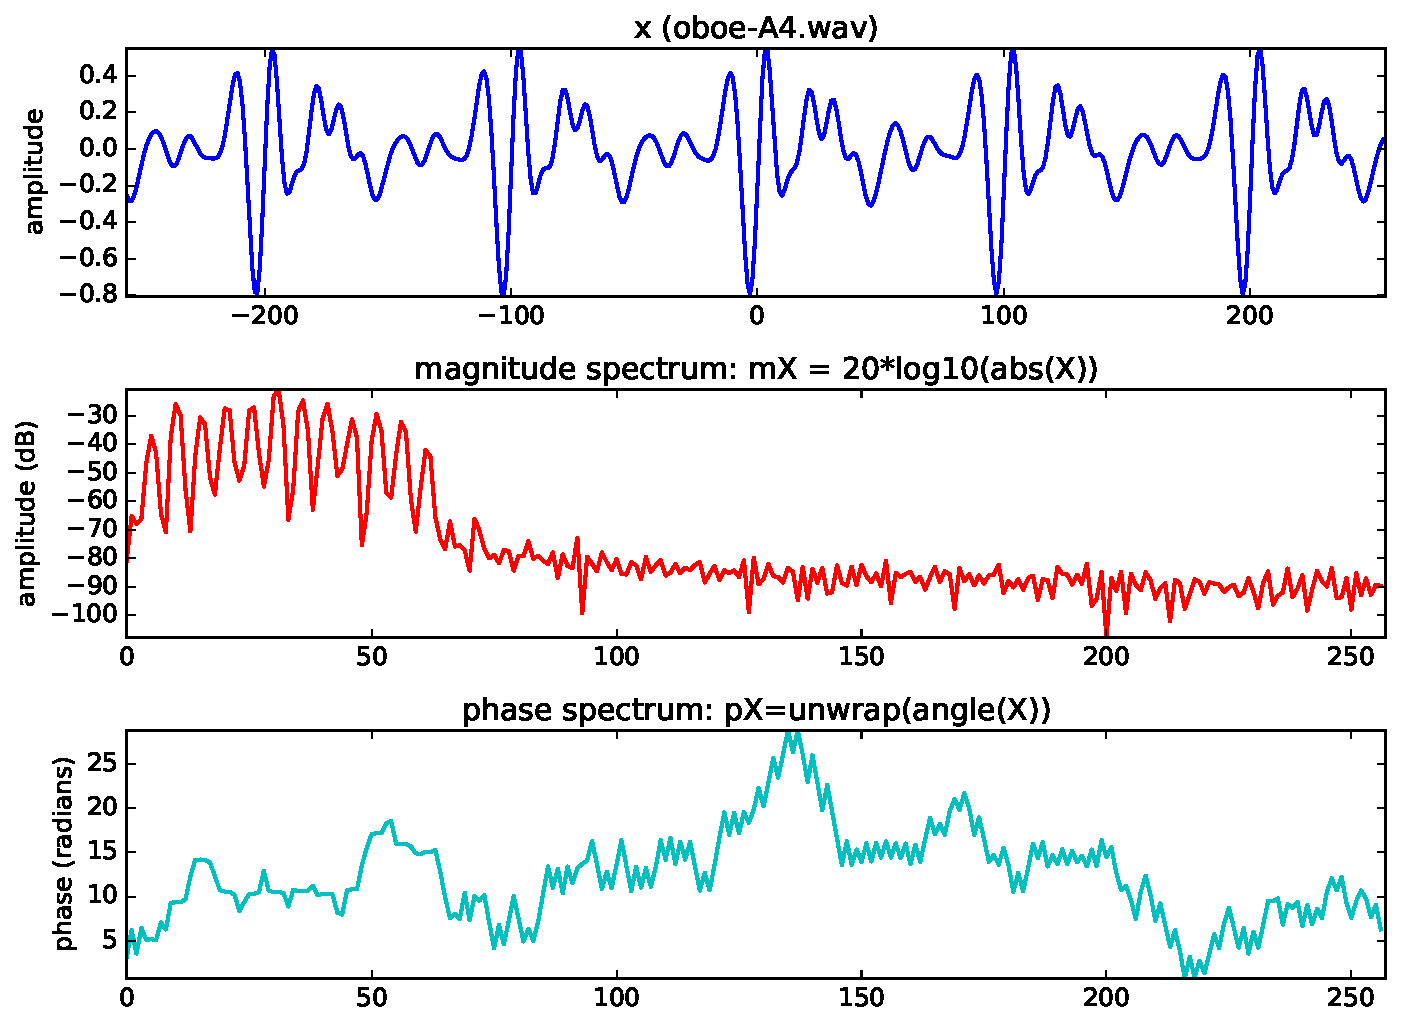
\includegraphics[width=3.0 in]{figuras/Fourier/spectrum_oboe.pdf}
\label{spectrum_oboe}
}
\subfigure{b)
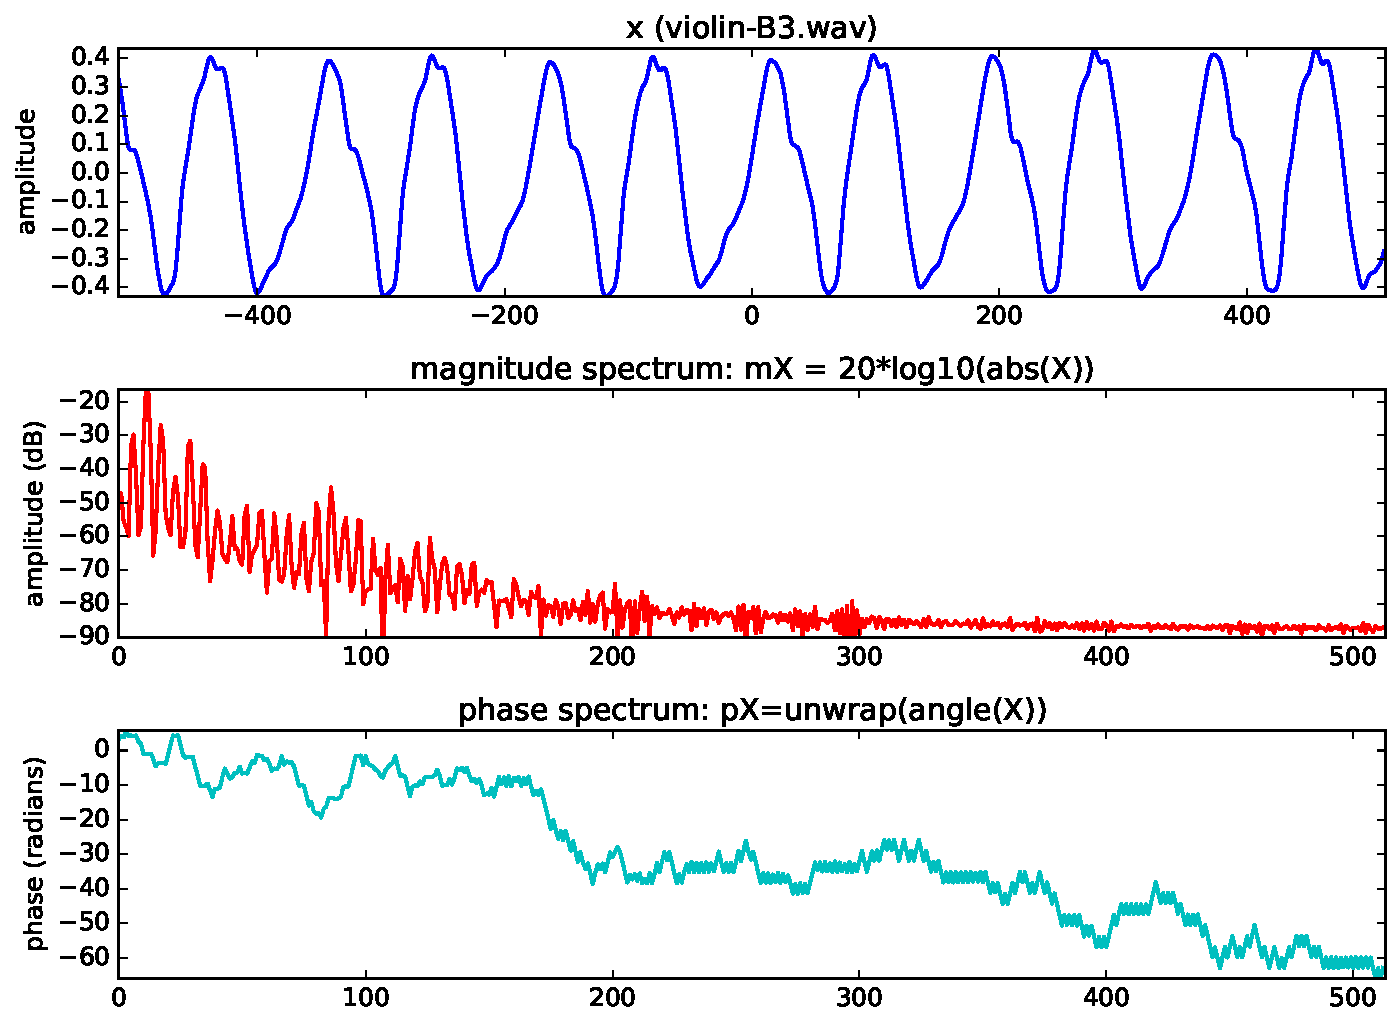
\includegraphics[width=3.0 in]{figuras/Fourier/spectrum_violino.pdf}
\label{spectrum_violino}
}
\caption[Transformada de Fourier do obo� e violino.]{ An�lise do som de um instrumento musical. No gr�fico de cima est� o som original. No gr�fico do meio est� a amplitude da transformada de Fourier, mostrando as frequ�ncias. No gr�fico de baixo est� a fase. \subref{spectrum_oboe} Obo�. \subref{spectrum_violino} Violino. Fonte: \url{https://github.com/MTG/sms-tools}.}
\end{figure}


{\noindent\def\stackalignment{l}% code from https://tex.stackexchange.com/a/195118/101651
    \stackunder[0pt]{\colorbox{cyan}{\textcolor{white}{\textbf{\LARGE Problemas}}}}{\textcolor{lightcyan}{\rule{\linewidth}{2pt}}}\medskip}



\begin{problema}
{\color{red}\Keyboard} Calcule a transformada r�pida de Fourier da fun��o $y(t) = \cos \omega t$ e fa�a o gr�fico, como na figura \ref{grafico_FFT_sin2}.
\end{problema}

\begin{problema}
{\color{red}\Keyboard} Refa�a o gr�fico da figura \ref{spectrum_oboe} com o som de outros dois instrumentos. Use alguns dos sons dispon�veis no curso do Prof. Xavier Serra: \url{https://github.com/MTG/sms-tools/tree/master/sounds}.
\end{problema}

{\noindent\def\stackalignment{l}{\textcolor{lightcyan}{\rule{\linewidth}{2pt}}}\medskip}




\chapter{Equa��es diferenciais parciais}  \label{capeqdifeparciais}




\section{Classifica��o e aplica��es na F�sica}

A din�mica de muitos sistemas f�sicos envolve derivadas segundas tais como acelera��o em mec�nica cl�ssica e energia cin�tica em mec�nica qu�ntica. Al�m disso as equa��es diferenciais (EDs) resultantes s�o fun��o tanto do tempo quanto das coordenadas espaciais. Essas equa��es cujas derivadas s�o em rela��o a mais de uma vari�vel s�o chamadas de Equa��es Diferenciais Parciais (EDP). V�rios dos resultados para EDO s�o v�lidos para EDP: princ�pio da superposi��o. As EDPs s�o classificadas em 3 grandes tipos, como mostra a tabela \ref{tiposdeEDPs}. V�rios exemplos desses tipos tem aplica��o na f�sica, como mostra a tabela \ref{aplicacoesfisica}\footnote{Equa��es de ordem maior que 2 tamb�m pode aparecer como $(\nabla^2)^2 \psi = 0$, por�m s�o bem raras e n�o ser�o discutidos aqui.}.
	
\begin{table}[h!]
\setlength{\arrayrulewidth}{1.0pt}
\centering
\arrayrulecolor{blue}
\renewcommand{\arraystretch}{2.0}% Spread rows out...
\begin{tabular}{ c | c | c | c }
\hline \hline
Nome  & El�ptica & Parab�lica & Hiperb�lica  \\
\hline Termos  &  $\nabla^2$ ou $\nabla^2 + \dfrac{1}{c}\dfrac{\partial^2}{\partial t^2}$  & $\nabla^2 + a\dfrac{\partial}{\partial t}$ & $\nabla^2 - \dfrac{1}{c}\dfrac{\partial^2}{\partial t^2}$  \\
\hline Exemplos & Eq. de Laplace e Poisson & Eq. de Difus�o & Eq. de Onda \\
\hline
\hline
\end{tabular}
\caption[EDPs el�pticas, parab�licas e hiperb�licas]{Defini��es de EDPs el�pticas, parab�licas e hiperb�licas.}
\label{tiposdeEDPs}
\end{table}



\begin{table}[h!]
\setlength{\arrayrulewidth}{1.0pt}
\centering
\arrayrulecolor{blue}
\renewcommand{\arraystretch}{2.0}% Spread rows out...
\begin{tabular}{ c | c | c  }
\hline \hline
Nome  & Equa��o & Aplica��es  \\
\hline Eq. de Laplace  &  $\nabla^2 \psi=0$  & eletrost�tica e magnetost�tica  \\
\hline Eq. de Poisson  & $\nabla^2 \psi=-\rho / \varepsilon_0$ & eletrost�tica e gravita��o \\
\hline Eq. de Helmholtz & $\nabla^2 \psi \pm k^2 \psi=0$ & elasticidade, ac�stica e ondas \\
\hline Eq. de Difus�o & $\nabla^2 \psi (t, \textbf{r}) = \dfrac{1}{a^2} \dfrac{\partial \psi}{\partial t}$ & difus�o de calor \\
\hline Eqs. de Maxwell & $\vec{\nabla} \cdot$ e $\vec{\nabla} \times$  & eletromagnetismo \\ 
\hline Eq. de Schrodinger & $-\dfrac{\hbar^2}{2m} \nabla^2 \psi + V(x) \psi = i\hbar \dfrac{\partial \psi}{\partial t}$ & mec�nica qu�ntica \\
\hline Eq. de Schrod. it & $-\dfrac{\hbar^2}{2m} \nabla^2 \psi + V(x) \psi = E\psi$ & mec�nica qu�ntica \\
\hline Eq. de Onda Generalizada & $ \partial^{\mu}\partial_{\mu} \psi(x) =  \left[ \dfrac{1}{c^2} \dfrac{\partial^2 \psi}{\partial t^2} - \nabla^2 \right] \phi = 0$ & eltrodin�mica \\
\hline Klein-Gordon & $\partial^{\mu}\partial_{\mu} \psi(x) = -\mu^2 \psi(x)$ & eq. de onda relativ�stica \\
\hline 
\hline
\end{tabular}
\caption[EDPs em f�sica]{EDPs importantes em f�sica. Schrod. it significa Schrodinger independente do tempo.}
\label{aplicacoesfisica}
\end{table}

De maneira geral os m�todos de solu��o podem ser classificados como:
\begin{itemize}
\item Separa��o de Vari�veis: uma ED parcial � convertida em um conjunto de EDs ordin�ria, sendo ent�o mais f�cil de resolver. Algumas constantes relacionam as diferentes EDOs sendo os autovalores dos operadores. Este m�todo � relacionado com as simetrias da EDP e seu grupo de transforma��es.
\item Fun��o de Green: neste m�todo uma EDP n�o homog�nea � convertida em uma equa��o integral.
\item M�todos num�ricos: atrav�s da aproxima��o das derivadas (diferen�as finitas por exemplo) � poss�vel converter uma EDP e uma equa��o alg�brica. Por�m, m�todos num�ricos se tornarm essenciais apenas com o advento dos computadores, os quais permitem efetuar quantos c�lculos forem necess�rios para se chegar na precis�o desejada.
\item Outros: v�rios outros m�todos anal�ticos de menor import�ncia tamb�m s�o utilizados, como transformada integral.
\end{itemize}


\subsection{Condi��es de contorno}

Um problema f�sico que consiste em uma EDP � resolvido completamente quando a solu��o encontrada satisfaz as condi��es de contorno (CC). Em geral essas condi��es s�o valores das fun��es em quest�o em algum tempo ou posi��o. Tr�s tipos principais de condi��es de contorno (CC) s�o utilizados em f�sica:
\begin{itemize}
\item CC de Cauchy: o valor da fun��o e sua derivada normal s�o especificados em alguma borda do sistema. Por exemplo em eletrost�tica o potencial $\varphi$ e a componente normal do campo el�trico normal $\textbf{E}_n$.
\item CC de Dirichlet: Apenas o valor da fun��o � especificado no contorno.
\item CC de Neumann: a derivada normal (gradiente normal) da fun��o � especificado. No caso eletrost�tico isso seria novamente $\textbf{E}_n$, e assim, a densidade de carga superficial.
\end{itemize}


\begin{table}[h!]
\setlength{\arrayrulewidth}{1.0pt}
\centering
%\renewcommand{\arraystretch}{2.0}% Spread rows out...
\arrayrulecolor{blue}
\begin{tabular}{ c | c c c }
\hline 
\hline & & \textbf{Tipos de EDP} \\
\textbf{Cond. de Contorno}  & \textbf{el�ptica} & \textbf{hiperb�lica} & \textbf{parab�lica}  \\
\hline Cauchy & & & \\
 superf�cie aberta & sem solu��o f�sica  & solu��o �nica e est�vel & muito restritiva \\
 sup. fechada & muito restritiva & muito restritiva & muito restritiva \\
\hline Dirichlet sup. aberta & insuficiente & insuficiente & solu��o �nica e est�vel \\
\hline Dirichlet sup. fechada & solu��o �nica e est�vel & v�rias solu��es & muito restritiva \\
\hline Neumann sup. aberta & insuficiente & insuficiente & solu��o �nica e est�vel \\
\hline Neumann sup. fechada & solu��o �nica e est�vel & v�rias solu��es & muito restritiva \\
\hline
\hline
\end{tabular}
\caption[Condi��es de contorno]{sup. significa superf�cie.}
\label{tiposcondcontorno}
\end{table}




  
  \begin{tcolorbox}[breakable,pad at break*=1mm,colback=blue!5!white,colframe=DarkGreen!75!black,title=Um pouco de hist�ria.]
  A letra $d$ para indicar a derivada como em $\slfrac{d}{dt}$ foi introduzida em 1675 pelo matem�tico alem�o Gottfried Leibniz. J� o s�mbolo curvado $\partial$ para indicar a derivada parcial foi introduzido em 1770 pelo matem�tico franc�s Marquis de Condorcet. Depois de tamb�m usado por Adrien-Marie Legendre e Carl Jacobi o s�mbolo se tornou padr�o. J� o s�mbolo da diferencial inexata $\bar{d}$ s� foi introduzido em 1875 por Carl Neumann. 
\end{tcolorbox}




\section{Separa��o de vari�veis em coordenadas cartesianas}


Come�amos por resolver a Eq. de Laplace $\nabla^2 \psi (\textbf{r}) = 0$, a qual pode ser resultado de diversas possibilidades, uma vez que $\nabla^2$ aparece em diversos tipos de EDP. Em coordenadas cartesianas temos:
\begin{equation}
\dfrac{\partial^2 \psi}{\partial x^2} + \dfrac{\partial^2 \psi}{\partial y^2} + \dfrac{\partial^2 \psi}{\partial z^2} = 0. \label{skwjwkjwekhh}
\end{equation}
A forma simples e tradicional de se resolver essa EDP � convert�-la em 3 EDOs supondo separa��o de vari�veis:
\begin{equation}
\psi(x,y,z) = X(x)Y(y)Z(z). \label{separaiviakri}
\end{equation}
Essa suposi��o � v�lida? Apenas a tentativa pode dizer: se encontrarmos uma solu��o, a tentativa � v�lida. Substituindo a Eq. \ref{separaiviakri} na Eq. \ref{skwjwkjwekhh} temos:
\begin{equation}
YZ \dfrac{d^2 X}{dx^2} + XZ\dfrac{d^2 Y}{d y^2} + XY\dfrac{d^2 Z}{dz^2} = 0. \nonumber
\end{equation}
Repare que como agora as derivadas s�o de fun��es de uma vari�vel apenas, as derivadas s�o totais. Dividindo tudo por $\psi = XYZ$ e rearranjando:
\begin{equation}
\dfrac{1}{X} \dfrac{d^2 X}{d x^2} = - \dfrac{1}{Y} \dfrac{d^2 Y}{d y^2} - \dfrac{1}{Z}\dfrac{d^2 Z}{d z^2}. \label{slskdjfksmzmz}
\end{equation}
A parte esquerda desta equa��o s� depende de $x$ enquanto a parte direita depende de $y$ e $z$. Duas fun��es diferentes de vari�veis diferentes s� podem ser iguais se ambas forem iguais a uma constante. A escolha desta constante � completamente arbitr�ria e em princ�pio h� uma infinidade delas que permitem encontrar uma solu��o. Por�m, temos tamb�m de procurar uma constante que seja adequada em termos do problema f�sico que estamos resolvendo. Escolhemos a constante tal que:
\begin{equation}
\dfrac{1}{X} \dfrac{d^2 X}{d x^2} = -l^2, \qquad \qquad - \dfrac{1}{Y} \dfrac{d^2 Y}{d y^2} - \dfrac{1}{Z}\dfrac{d^2 Z}{d z^2} = -l^2 \label{skwjhwkjkjqkjkj}
\end{equation}
Regorganizando a Eq. da direita:
\begin{equation}
\dfrac{1}{Y} \dfrac{d^2 Y}{d y^2} = l^2 - \dfrac{1}{Z}\dfrac{d^2 Z}{d z^2}.  \nonumber
\end{equation}
Veja que agora temos apenas duas vari�veis diferentes. Temos novamente que usar o argumento de que duas fun��es diferentes de vari�veis diferentes s� podem ser iguais se ambas forem constantes:
\begin{equation}
\dfrac{1}{Y} \dfrac{d^2 Y}{d y^2} = -m^2, \qquad \qquad \dfrac{1}{Z}\dfrac{d^2 Z}{d z^2} = n^2, \label{sksjwnwmnwk}
\end{equation}
onde $n^2 = l^2 + m^2$. Veja que agora temos 3 EDOs (Eqs. \ref{skwjhwkjkjqkjkj} e \ref{sksjwnwmnwk}) utilizando tr�s constantes diferentes.




\subsection{Difus�o de calor}


Em um s�lido com uma distribui��o de temperatura independente do tempo $T(\textbf{r})$, o calor flui da regi�o com maior temperatura para a regi�o de menor temperatura. O fluxo de calor � da forma $\textbf{j} = - \kappa \vec{\nabla} T(\textbf{r})$, onde $\kappa$ � a condutividade do meio. Se h� uma fonte de calor o fluxo ter� uma varia��o dada por $\vec{\nabla} \cdot \textbf{j} = -  \kappa \nabla^2 T(\textbf{r})$. J� quando h� uma varia��o da temperatura com o tempo � por que energia est� sendo cedida ou tirada do sistema. A equa��o de difus�o t�rmica ent�o nesse caso fica:
\begin{equation}
\dfrac{\partial T}{\partial t} = \dfrac{\kappa}{\sigma \rho} \nabla^2 T. 
\end{equation} 


\subsubsection{Sem depend�ncia temporal}


No caso independente do tempo $\partial T /\partial t = 0$, a equa��o de difus�o se torna a Eq. de Laplace, a qual vamos resolver agora. Seja um s�lido paralelep�pedo cujas as arestas estejam paralelas aos eixos coordenados com um dos seus v�rtices na origem do sistema. Suponhamos que o s�lido � finito nas dire��es $x$ e $y$ mas infinito na dire��o $z>0$\footnote{Pode n�o parecer, mas essa aproxima��o � muito comum. Ela � v�lida quando o comprimento ao longo de $z$ � grande e estamos interessados na temperatura apenas em uma das extremidades.}. Na parte de baixo do s�lido a condi��o de contorno para a temperatura � $T(x,y,z = 0)=T_0(x,y)$. Para encontrar a distribui��o de temperatura $T(\textbf{r})$ devemos resolver a Eq. de Laplace supondo separa��o de vari�veis como descrito na se��o anterior. As solu��es para $X(x)$ e $Y(y)$ (veja Eqs. \ref{skwjhwkjkjqkjkj} e \ref{sksjwnwmnwk}) s�o fun��es peri�dicas (seno e cosseno):
\begin{equation}
X_l(x) = A_l \cos lx + B_l \sin lx, \qquad \qquad Y_m(y) = C_m \cos my + D_m \sin my. \label{slkwjlkjwerop}
\end{equation}
J� a constante $n^2$ na equa��o de $Z(z)$ (Eq. \ref{sksjwnwmnwk}) � positiva, logo a solu��o ser� composta de exponenciais reais: $Z(z) = E_n e^{nz} + F_n e^{-nz}$. Como estamos assumindo o s�lido infinito para $z>0$, temos que $\lim_{z \rightarrow \infty} T(z) = 0$, logo descartamos a exponencial positiva $e^{nz}$ fazendo $E_n = 0$. A solu��o fica ent�o uma superposi��o de todas as solu��es poss�veis:
\begin{equation}
T(x,y,z) = \sum_{l=0}^{\infty} \sum_{m=0}^{\infty} \alpha_{lm} X_l(x) Y_m(y) e^{-nz}. \nonumber 
\end{equation}
Resta impor a condi��o de contorno $T(x,y,z = 0)=T_0(x,y)$:
\begin{equation}
T_0(x,y) = \sum_{l=0}^{\infty} \sum_{m=0}^{\infty} \alpha_{lm} X_l(x) Y_m(y).  \label{condcortondifus}
\end{equation}
Como $X(x)$ e $Y(y)$ s�o senos e cossenos, a Eq. \ref{condcortondifus} � satisfeita e os coeficientes $\alpha_{lm}$ s�o encontrados em fun��o de $T_0(x,y)$.

\begin{SCfigure}
 \centering
\includegraphics[width=2.0 in]{figuras/EDP/retangulo_EDP.png}
\caption[Problema 2.]{Ret�ngulo no plano $xy$. Exemplo \ref{capeqdifeparciais}.\ref{eqdifusaoplanoxy}.}
\label{retangulo_EDP}
\end{SCfigure} %acertado

\begin{exemplo} \label{eqdifusaoplanoxy}
Suponha um ret�ngulo infinito no plano $xy$ e as condi��es de contorno como indicado na figura \ref{retangulo_EDP}. Encontre a solu��o $T(x,y)$.
\tcblower
A Eq. de Laplace neste caso fica $\nabla^2 = \dfrac{\partial^2 T}{\partial x^2} + \dfrac{\partial^2 T}{\partial y^2} = 0$. Para resolver usamos a mesma estrat�gia para o caso 3D (veja Eq. \ref{skwjwkjwekhh}): $T(x,y) = X(x)Y(y)$. Seguindo o mesmo procedimento at� a Eq. \ref{skwjhwkjkjqkjkj} obtemos:
\begin{equation}
\dfrac{1}{X} \dfrac{d^2 X}{d x^2} = -k^2, \qquad \qquad \dfrac{1}{Y}\dfrac{d^2 Y}{d y^2} = k^2. \nonumber
\end{equation}
As solu��es s�o da forma:
\begin{equation}
X_k(x) = A_k \cos kx + B_k \sin kx, \qquad \qquad Y_k(y) = C_k e^{ky} + D_k e^{-ky}. \label{skwjjzzzzxc}
\end{equation}
Agora devemos impor as condi��es de contorno. Da figura \ref{retangulo_EDP} temos $T(x=0) = 0$. Logo $X_k(0) = A_k$, o que implica que $A_k=0$. Al�m disso $T(x=a) = 0$, logo $X(a) = B_k \sin ka =0$, o que implica:
\begin{equation}
k = \dfrac{n\pi x}{a}, \qquad \qquad \qquad n = 1, 2, 3, ... \label{skwjwbwbwbwb}
\end{equation}
Da mesma forma $T(y = +\infty) = 0$. Como $\lim_{y \rightarrow +\infty} e^{-ky} = 0$ temos que impor $C_k=0$. A solu��o geral � a soma para todos os valores de $n$:
\begin{equation}
T(x,y) = \sum_{n=1}^{\infty} b_n e^{-n\pi y/a} \sin \dfrac{n \pi x}{a}.
\end{equation}
Por �ltimo falta a condi��o de contorno $T(x,y=0) = T_0 = 100$ graus. Da solu��o geral temos:
\begin{equation}
T_0 = \sum_{n=1}^{\infty} b_n \sin \dfrac{n \pi x}{a},
\end{equation}
que � uma expans�o em s�rie de Fourier (veja Eq. \ref{seriefoueirseconss}). Da Eq. \ref{coefisenofouier} os coeficientes s�o:
\begin{equation}
b_n = \dfrac{2}{a} \int_0^a T_0 \sin  \dfrac{n \pi x}{a} dx = \dfrac{2T_0}{a} 
\end{equation}
\end{exemplo}






\subsubsection{Com depend�ncia temporal}

Vamos agora resolver a equa��o de difus�o t�rmica incluindo a depend�ncia temporal. Considerando um meio anisotr�pico a Eq. de difus�o t�rmica mais geral �:
\begin{equation}
\dfrac{\partial T}{\partial t} = a^2\dfrac{\partial^2 T}{\partial x_1^2} +b^2 \dfrac{\partial^2 T}{\partial y_1^2} + c^2\dfrac{\partial^2 T}{\partial z_1^2}, \label{slwkjwkjwlkjw}
\end{equation}
onde $a$, $b$ e $c$ s�o as taxas de difus�o ao longo dos eixos principais. Quando essas constantes s�o diferentes, podemos redefinir cada coordenada da forma $x_1 = ax$, $y_1 = by$ e $z_1 = c z$ de forma que a Eq. de difus�o t�rmica fica:
\begin{equation}
\dfrac{\partial T}{\partial t} = \dfrac{\partial^2 T}{\partial x^2} + \dfrac{\partial^2 T}{\partial y^2} + \dfrac{\partial^2 T}{\partial z^2} = 0.
\end{equation}

Come�amos com o caso unidimensioal:
\begin{equation}
\dfrac{\partial T}{\partial t} = a^2\dfrac{\partial^2 T}{\partial x^2}, \label{eqdifusaotermi1d}
\end{equation}
onde agora $a$ � a condutividade do meio. Usamos novamente a separa��o de vari�veis, fazemos a seguinte solu��o tentativa: $T(x,t) = e^{\alpha x} e^{\beta t}$, o que retorna $\beta = a^2 \alpha^2$. Fisicamente esperamos que a solu��o no tempo decaia para zero em tempos longos e ent�o fazemos $\alpha = i \omega$ para $\omega$ real. A solu��o fica 
\begin{equation}
T = e^{i \omega x} e^{ -\omega^2 a^2t} =  (A\cos \omega x + B \sin \omega x)e^{ -\omega^2 a^2t}. \label{spolwkjzxcvbm}
\end{equation}
As constantes $A$, $B$ (derivada dupla em $x$) e $\omega$ (derivada temporal) devem satisfazer as condi��es de contorno. Por�m, outra possibilidade � fazer um somat�rio tamb�m em $\omega$, que se torna uma intergral:
\begin{equation}
T(x,t) =  \int \left[ A(\omega)\cos \omega x + B(\omega) \sin \omega x \right]  e^{ -\omega^2 a^2t} d\omega. \nonumber
\end{equation}
Esta express�o � geral o suficiente para satisfazer as condi��es de contorno em $t=0$.

\begin{exemplo}
Seja uma barra unidimensional cuja temperatura inicial em $t=0$ � $T(x,t=0)=T_0=1$ no intervalo $\vert x \vert < 1$ e 0 fora dele. Encontre a temperatura em fun��o do tempo em toda a barra.
\tcblower
Em $t=0$ a equa��o de difus�o t�rmica se reduz a equa��o de Laplace cuja solu��o espacial � formada por senos e cossenos (veja Eq. \ref{slkwjlkjwerop}). Como precisamos que $T(x = \pm 1,0) = 0$ eliminamos o termo em seno de modo que $\cos lx = \cos \pm l = 0$. Isso implica em $l=n\pi/2$ para $n$ �mpar. A solu��o fica $T_n(x,0) = \cos n\pi x/2$. Por�m, como precisamo que $T=1$ no intervalo $\vert x \vert < 1$, a solu��o fica descrita pela S�rie de Fourier:
\begin{equation}
T(x,0) = \sum_{n=1}^{\infty} T_n(x,0) = \sum_{n=1}^{\infty} a_l \cos n\pi x/2 = 1. \nonumber 
\end{equation}
Os coeficientes s�o:
\begin{equation}
a_n = \int_{-1}^1 1 \cos \dfrac{n \pi x}{2}dx = \dfrac{4}{n\pi} \sin \dfrac{n\pi}{2}  = 
 \left\{
\begin{array}{rl}
\dfrac{4(-1)^m}{(2m+1)\pi}& \text{se } n = 2m+1  \\
0 & \text{se } n = 2m
\end{array} 
\right. 
\end{equation}

Para $t>0$ a Eq. a ser resolvida � a Eq. \ref{eqdifusaotermi1d} cuja solu��o � da forma da Eq. \ref{spolwkjzxcvbm}. Basta ent�o multiplicar a s�rie encontrada pela exponencial temporal:
\begin{equation}
T(x,t) = \dfrac{4}{\pi} \sum_{n=1}^{\infty} \dfrac{(-1)^m}{2m+1} \cos \left[ (2m+1)\dfrac{\pi x}{2} \right] \exp \left\lbrace  -t\left[ (2m+1)\dfrac{\pi a}{2} \right]^2\right\rbrace  . \nonumber 
\end{equation}
\end{exemplo}


\subsubsection{3 dimens�es}

Em 3 dimens�es a solu��o tentaiva � $T = \exp \left(  \dfrac{i}{a}  \textbf{k} \cdot \textbf{r} + \beta t\right)$, o que leva a $-\beta = -\vert \textbf{k} \vert^2 = -k^2$ quando substitu�da na Eq. \ref{slwkjwkjwlkjw}. O que leva a seguinte equa��o:
\begin{equation}
\dfrac{\partial^2 T}{\partial x^2} + \dfrac{\partial^2 T}{\partial y^2} + \dfrac{\partial^2 T}{\partial z^2} + k^2 T = 0, \nonumber
\end{equation}
a qual � chamada de Eq. de Helmholtz. Esta equa��o pode ser resolvida tamb�m por separa��o de vari�veis.




\subsection{M�todo das Diferen�as Finitas}


A solu��o num�rica consiste em aproximar as derivadas por diferen�as. Por exemplo, a primeira derivada pode ser escrita como:
\begin{equation}
\dfrac{\partial T}{\partial x} \approx  \dfrac{T (x_{i+1}) - T(x_i)  }{\Delta x}. \nonumber
\end{equation}
Para simplificar a nota��o usamos: $T(x_i) = T_i$. Essa � a derivada no ponto intermedi�rio entre $x_i$ e $x_{i+1}$. Da mesma forma podemos aproximar a derivada no ponto $x_{i-1/2}$:
\begin{equation}
\dfrac{\partial T}{\partial x} \approx  \dfrac{T_i - T_{i-1}  }{\Delta x}. \nonumber
\end{equation}
Por�m, para resolver a Eq. de Laplace precisamos de uma aproxima��o para a segunda derivada. Usaremos ent�o a primeira derivada nas posi��es $i \pm 1/2$:
\begin{equation}
\dfrac{\partial^2 T}{\partial x^2} \approx  \dfrac{T_{i+1/2} - T_{i-1/2}  }{\Delta x^2} = \dfrac{T_{i+1} - 2T_i + T_{i-1} }{(\Delta x )^2} \label{aproderivadasegund} 
\end{equation}
Como essa express�o envolve $\Delta x^2$, dizemos que ela � boa at� terceira ordem em $\Delta x$. Agora, para resolver a equa��o geral \ref{eqlaplacegeral3D}, aproximamos cada derivada segunda pela express�o na Eq. \ref{aproderivadasegund}. O que nos d�:
\begin{equation}
T_{i,j,k} = \frac{1}{6} \left( T_{i+1,j,k} + T_{i-1,j,k} + T_{i,j+1,k} + T_{i,j-1,k} + T_{i,j,k+1} + T_{i,j,k-1} \right). \nonumber 
\end{equation}
A eq. de Laplace � �til tanto para descrever a distriui��o de temperatura pela difus�o t�rmica como a distribui��o de potencial el�trico em uma regi�o sem carga el�trica. 



\begin{codigo}
Como exemplo, vamos calcular a distribui��o de temperatura em um quadrado bidimensional. A eq. de Laplace fica:
\begin{equation}
\dfrac{\partial^2 T}{\partial x^2} + \dfrac{\partial^2 T}{\partial y^2} = 0. \nonumber 
\end{equation}
Aproximando as derivadas por diferen�as finitas teremos:
\begin{equation}
\dfrac{T_{i+1,j} - 2T_{i,j} + T_{i-1,j} }{(\Delta x )^2} + \dfrac{T_{i,j+1} - 2T_{i,j} + T_{i,j+1} }{(\Delta y )^2} = 0. \nonumber
\end{equation}
de forma que:
\begin{equation}
T_{i,j} = \frac{1}{4} \left( T_{i+1,j} + T_{i-1,j} + T_{i,j+1} + T_{i,j-1} \right). \nonumber 
\end{equation}

O c�lculo em si da tempratura consiste em calcular individualmente em cada ponto da rede, utilizando os valores dos pontos vizinhos. Um trecho do c�digo �:
\begin{lstlisting}
for iteration in range(0, Niter):
	for i in range(1, lenX-1, delta):
		for j in range(1, lenY-1, delta):
			T[i, j] = 0.25 * (T[i+1][j] + T[i-1][j] + T[i][j+1] + T[i][j-1])
\end{lstlisting}
Veja que os dois \verb|for| internos em \verb|i| e \verb|j| s�o suficientes para calcular a fun��o \verb|T[i,j]| em todo o espa�o. Por�m, cada vez que � calculado em todo o espa�o, a solu��o converge. Assim, s�o necess�rio v�rios c�lculos at� confirmar a converg�ncia. Essa � a fun��o do primeiro \verb|for| na vari�vel \verb|iteration| que n�o aparece na conta em si: apenas repetir o c�lculo de \verb|T[i,j]| \verb|Niter| vezes. Repare que o n�mero de itera��es \verb|Niter| tem que ser suficiente para que a converg�ncia seja obtida. Assim, nos primeiros c�lculo � necess�rio ir aumentando o seu valor at� ser verificado que a solu��o de fato convergiu.  

Na figura \ref{difusao_temperatura1} est� o resultado do c�lculo. O c�digo que faz o c�lculo e gera a figura est� Github\footnote{\url{https://github.com/paulofreitasgomes/computationalphysics/blob/master/Termodinamica/laplace_temperatura.py}.}.
\end{codigo}


\begin{SCfigure}
 \centering
\includegraphics[trim={0.3in 0.0in 0.7in 0.2in},clip, width=4.0 in]{figuras/EDP/difusao_temperatura1.pdf}
\caption{Gr�fico da temperatura no dom�nio.}
\label{difusao_temperatura1}
\end{SCfigure} %acertado
 %trim={<left> <lower> <right> <upper>}



\subsection{Potencial el�trico}

O potencial el�trico $V(\textbf{r})$ em uma regi�o que n�o cont�m cargas el�tricas tamb�m segue a Eq. de Laplace: $\nabla^2 V = 0$\footnote{Obviamente, se n�o h� carga em todo o espa�o o potencial � zero. Por�m, estamos interessados em uma regi�o onde n�o h� carga mas que esteja pr�ximo a alguma distribui��o de carga de forma que $V \neq 0$.}. Vamos ilustrar este tema com exemplos.

\begin{SCfigure}
 \centering
\includegraphics[width=3.0 in]{figuras/EDP/tubo_metalico_3d.png}
\caption[Tubo met�lico do exemplo \ref{capeqdifeparciais}.\ref{exetuobmetalidos}.]{Ilustra��o do tubo met�lico ao longo de $x$ do Exemplo \ref{capeqdifeparciais}.\ref{exetuobmetalidos}.}
\label{tubo_metalico_3D}
\end{SCfigure} %acertado

\begin{exemplo} \label{exetuobmetalidos}
Um longo tubo met�lico (figura \ref{tubo_metalico_3D}) de se��o transversal retangular (lados $a$ e $b$) � aterrado ($V=0$) com exce��o da face $x=0$. Encontre o potencial dentro do tubo.

\tcblower

Trata-se de um problema 3D e a Eq. a ser resolvida � a Eq. \ref{skwjwkjwekhh}. As condi��es de contorno s�o:
\begin{enumerate}
\item $V=0$ se $y=0$ e se $y=a$. 
\item $V=0$ se $z=0$ e se $z=b$. 
\item $V \rightarrow 0 $ se $x \rightarrow \infty$.
\item $V = V_0(y,z)$ se $x=0$. 
\end{enumerate}
Supondo separa��o de vari�veis chegamos na Eq. \ref{slskdjfksmzmz}. Igualamos ent�o a fun��o de cada vari�vel a uma constante:
\begin{equation}
\dfrac{1}{X} \dfrac{d^2 X}{d x^2} = C_1, \qquad \dfrac{1}{Y} \dfrac{d^2 Y}{d y^2} = C_2, \qquad \dfrac{1}{Z}\dfrac{d^2 Z}{d z^2} = C_3, \qquad C_1+C_2+C_3=0. \nonumber
\end{equation}
Agora devemos fazer a escolha adequada das constantes. Como o potencial vai para zero em $x \rightarrow \infty$ fazemos $C_1$ positivo de modo que as solu��es sejam exponenciais reais (veja Eq. \ref{sjwjhhhhh}). Por outro lado fazemos $C_2$ e $C_3$ negativos para que as solu��es sejam oscilat�rias e satisfazer as condi��es de contorno:
\begin{equation}
C_2 = -k^2, \qquad \qquad C_3 = -l^2, \qquad \qquad C_1 = k^2 +l^2.
\end{equation} 
Assim a Eq. de Laplace fica
\begin{equation}
\dfrac{1}{X} \dfrac{d^2 X}{d x^2} = k^2 + l^2, \qquad \dfrac{1}{Y} \dfrac{d^2 Y}{d y^2} = -k^2, \qquad \dfrac{1}{Z}\dfrac{d^2 Z}{d z^2} = -l^2, \qquad C_1+C_2+C_3=0, \nonumber
\end{equation}
com as seguintes solu��es
\begin{eqnarray}
X(x) &=& A \exp \left( x \sqrt{k^2 + l^2} \right) + B \exp \left( -x \sqrt{k^2 + l^2} \right), \\
Y(y) &=& C \sin ky + D \cos ky, \qquad \qquad Z(z) = E \sin lz + F \cos lz.  
\end{eqnarray}
Aplicando as condi��es de contorno temos: 
\begin{itemize}
\item [1] implica em $D = 0$ e $k =n\pi/a$ com $n$ sendo inteiro positivo. 
\item [2] implica em $F = 0$ e $l =m\pi/a$ com $m$ sendo inteiro positivo. 
\item [3] implica em $A=0$.
\end{itemize}
A solu��o ent�o toma a forma:
\begin{equation}
V_{n,m}(\textbf{r}) = X(x)Y(y)Z(z) = C \sin (n\pi y/a) \sin (m\pi z/b) \exp \left(-\pi  x \sqrt{(n/a)^2 + (m/b)^2} \right). \nonumber 
\end{equation}
Como a Eq. de Laplace � linear, a solu��o geral � uma soma destas solu��es:
\begin{equation}
V(\textbf{r}) = \sum_{n=1}^{\infty} \sum_{m=1}^{\infty} C_{n,m} \sin (n\pi y/a) \sin (m\pi z/b) \exp \left(-\pi  x \sqrt{(n/a)^2 + (m/b)^2} \right). \label{slkjdfpppp}
\end{equation}
Agora falta apenas uma condi��o de contorno [4]:
\begin{equation}
V(x=0,y,z) = \sum_{n=1}^{\infty} \sum_{m=1}^{\infty} C_{n,m} \sin (n\pi y/a) \sin (m\pi z/b) = V_0(y,z). \nonumber
\end{equation}
Esta equa��o pode ser satisfeita pois a fun��o seno forma um conjunto completo. Multiplicando por $\sin (p\pi y/a) \sin (q \pi z/b)$ e integrando temos:
\begin{eqnarray}
 \sum_{n=1}^{\infty} \sum_{m=1}^{\infty} C_{n,m} \int_0^a \sin (n\pi y/a) \sin (p\pi y/a)dy \int_0^b \sin (m\pi z/b) \sin (q\pi z/b) \nonumber \\
  = \int_0^a \int_0^b V_0(y,z) \sin (p\pi y/a)dy \sin (q\pi z/b). \nonumber
\end{eqnarray}
Usando a Eq. \ref{conjcomplesenos}, sobra apenas os termos $n=p$ e $m=q$ de forma que:
\begin{equation}
C_{p,q} =  \dfrac{4}{ab} \int_0^a \int_0^b V_0(y,z) \sin (p\pi y/a)dy \sin (q\pi z/b) . \label{lsksjksmmzzzz}
\end{equation}
As Eqs. \ref{slkjdfpppp} e \ref{lsksjksmmzzzz} s�o a solu��o do problema.
\end{exemplo}


{\noindent\def\stackalignment{l}% code from https://tex.stackexchange.com/a/195118/101651
    \stackunder[0pt]{\colorbox{cyan}{\textcolor{white}{\textbf{\LARGE Problemas}}}}{\textcolor{lightcyan}{\rule{\linewidth}{2pt}}}\medskip}
    
\begin{problema} 
Resolva as eqs. diferenciais para $X(x)$ e $Y(y)$ (contida nas Eqs. \ref{skwjhwkjkjqkjkj} e \ref{sksjwnwmnwk}).
\end{problema}   
    

\begin{problema} 
a) Deduza as Eqs. \ref{skwjjzzzzxc}. b) Deduza a Eq. \ref{skwjwbwbwbwb}.
\end{problema}   


\begin{problema} 
Vamos agora considerar uma varia��o do problema descrito no exemplo \ref{capeqdifeordinaria}.\ref{eqdifusaoplanoxy}. Seja o ret�ngulo finito de lado $a$ na dire��o $x$ e $b$ na dire��o $y$. A condi��o de contorno agora deixa de ser $T(y = +\infty) = 0$ para ser $T(y = b) = 0$ \celsius. a) Mostre que a solu��o em $y$ agora fica $Y(y) = B \sinh k(b-y)$\footnote{$\sinh$ � a fun��o seno hiperb�lico definida na Eq. \ref{cossenohiper}.}. b) Mostre que a solu��o geral �:
\begin{equation}
T(x,y) = \sum_{n=1}^{\infty} B_n \sinh \dfrac{n \pi (b-y)}{a} \sin \dfrac{n \pi x}{a}.
\end{equation}
c) Considere agora a �ltima condi��o de contorno: $T(x,y=0) = T_0 = 100$ graus. Mostre que a solu��o final �:
\begin{equation}
T(x,y) = \sum_{n \quad \text{�mpar}}^{\infty} \dfrac{400}{n\pi \sinh 3n\pi} \sinh \dfrac{n \pi (b-y)}{a} \sin \dfrac{n \pi x}{a}.
\end{equation}
\end{problema}   


\begin{problema}
Mostre que existe apenas uma solu��o $u$ da Eq. de Laplace e que satisfaz as condi��es de contorno nas bordas. Dica: suponha que haja duas solu��es $u_1$ e $u_2$ e mostre que $u = u_1-u_2=0$ � zero nas bordas.
\end{problema}

\begin{problema} \label{proexetubmetalis}
Considere o exemplo \ref{capeqdifeordinaria}.\ref{exetuobmetalidos}. Seja $V_0(y,z) = V_0$ uma constante. Encontre os coeficientes $C_{n,m}$.
\end{problema}

\begin{problema} \label{problemacubometalico}
Um paralelep�pedo oco met�lico de lados $L_1$, $L_2$ e $L_3$ nas dire��es $x$, $y$ e $z$ (veja figura \ref{paralelepipedo_metalico}) tem 5 de suas faces aterradas (o que implica em potencial igual a zero). A face $z=L_3$ � isolada das outras e mantida a um potencial $V_0$. Encontre o potencial dentro da caixa.
\end{problema}

\begin{problema}
Mostre que o operador $\nabla^2 + k^2$ � linear, ou seja: $(\nabla^2 + k^2)(a_1 \psi_1 + a_2 \psi_2 ) = a_1 (\nabla^2 + k^2) \psi_1 + a_2 (\nabla^2 + k^2) \psi_2$.
\end{problema}

\begin{problema} \label{proprova3metl}
Uma part�cula de massa $m$ � confinada em uma caixa de lados $a$, $b$ e $c$. Na teoria da Mec�nica Qu�ntica, a part�cula � descrita pela fun��o de onda $\Psi(\textbf{r})$ que satisfaz a equa��o de Schr�dinger:
\begin{equation} 
-\dfrac{\hbar^2}{2m} \nabla^2 \Psi = E \Psi. \nonumber
\end{equation}
As condi��es de contorno exigem que $\Psi$ seja zero nas superf�cies da caixa. Estas condi��es imp�e restri��es nas constantes de separa��o e consequentemente na energia. a) Calcule a solu��o para as fun��es de onda $\Psi(\textbf{r})$ e as energias $E$. b) Calcule a energia do estado fundamental. c) Calcule a energia do primeiro estado excitado. Este estado � degenerado?
\end{problema}


{\noindent\def\stackalignment{l}{\textcolor{lightcyan}{\rule{\linewidth}{2pt}}}\medskip}

\begin{SCfigure}
 \centering
\includegraphics[width=2.0 in]{figuras/EDP/paralelepipedo_metalico.png}
\caption[Cubo met�lico do Problema \ref{capeqdifeparciais}.\ref{problemacubometalico}.]{Paralelep�pedo met�lico oco de lados $L_1$, $L_2$, e $L_3$ referente ao Problema \ref{capeqdifeparciais}.\ref{problemacubometalico}.}
\label{paralelepipedo_metalico}
\end{SCfigure} %acertado



\section{Separa��o de vari�veis em coordenadas cil�ndricas}


A equa��o de Laplace $\nabla^2 \psi (\textbf{r}) = 0$ em coordenadas cil�ndricas �:
\begin{equation}
\nabla^2 \psi (\textbf{r}) = \dfrac{1}{s} \dfrac{\partial }{ \partial s  } \left( s \dfrac{\partial \psi}{ \partial s } \right) + \dfrac{1}{s^2} \dfrac{\partial^2 \psi }{ \partial \varphi^2 } +  \dfrac{\partial^2 \psi }{ \partial z^2 } = 0. \nonumber
\end{equation}
Como antes assumimos $\psi( \textbf{r}) = P(s) \Phi (\varphi) Z(z)$, de modo que a eq. de Laplace fica:
\begin{equation}
\dfrac{ \Phi Z }{s} \dfrac{d }{ d s  } \left( s \dfrac{dP}{ d s } \right) + \dfrac{PZ}{s^2} \dfrac{d^2 \Phi }{ d \varphi^2 } + P \Phi \dfrac{d^2 Z }{ d z^2 } = 0. \label{skskwmmmmm}
\end{equation}
Repare que novamente todas as derivadas parciais agora se tornam derivadas totais, j� que cada fun��o depende de apenas uma vari�vel. Agora dividimos a Eq. \ref{skskwmmmmm} por $P(s) \Phi (\varphi) Z(z)$ e passamos o �ltimo termo para o lado direito da equa��o:
\begin{equation}
\dfrac{ 1 }{P s} \dfrac{d }{ d s  } \left( s \dfrac{dP}{ d s } \right) + \dfrac{1}{\Phi s^2} \dfrac{d^2 \Phi }{ d \varphi^2 } = - \dfrac{1}{Z} \dfrac{d^2 Z }{ d z^2 }. \label{sjsjs2229}
\end{equation}

Novamente, se duas fun��es diferentes de vari�veis diferentes s�o iguais, ambas tem que ser iguais a uma constante. Escolhemos uma constante tal que:
\begin{equation}
 \dfrac{1}{Z} \dfrac{d^2 Z }{ d z^2 } = k^2 Z. \label{sjsj2222}
\end{equation}
Esta equa��o � exatamente a Eq. \ref{sjwjhhhhh} com sinal positivo de modo que a solu��o � formada por exponenciais reais (Eq. \ref{hshs44333}):
\begin{equation}
Z(z) = A e^{kz} + B e^{-kz}. \label{eedede333}
\end{equation}

Uma vez encontrado a solu��o da parte em $z$, substituimos a Eq. \ref{sjsj2222} na Eq. \ref{sjsjs2229} e obtemos (ap�s multiplicar por $s^2$ e passar o termo em $\varphi$ para o lado direito): 
\begin{equation}
\dfrac{ s }{P } \dfrac{d }{ d s  } \left( s \dfrac{dP}{ d s } \right) + k^2 s^2 = -\dfrac{1}{\Phi } \dfrac{d^2 \Phi }{ d \varphi^2 }. \label{wwwwws2229}
\end{equation}
Para que essa equa��o seja v�lida � necess�rio igualar cada lado a uma constante. Escolhemos:
\begin{equation}
\dfrac{1}{\Phi } \dfrac{d^2 \Phi }{ d \varphi^2 } = n^2. \label{sjsjwh22}
\end{equation}
Esta equa��o � exatamente a Eq. \ref{sjwjhhhhh} com sinal negativo de modo que a solu��o � oscilat�ria (Eq. \ref{sjhwjhwghg}). Por�m, fisicamente $\varphi$ � um �ngulo azimutal (o mesmo em coordenadas esf�ricas) de modo que os �ngulos $\varphi$ e $\varphi + 2\pi$ correspondem a mesma posi��o angular. Assim, a fun��o $\Phi$ deve ter um �nico valor em cada: $\Phi (\varphi) = \Phi (\varphi + 2\pi)$, o que est� de acordo com a solu��o oscilat�ria.

Uma vez encontrada a solu��o para $\Phi$ falta agora apenas $P(s)$. Substituindo a Eq. \ref{sjsjwh22} na Eq. \ref{wwwwws2229} temos:
\begin{equation}
s  \dfrac{d }{ d s  } \left( s \dfrac{dP}{ d s } \right) + (k^2 s^2 -n^2)P = 0. \label{xxxxws2229}
\end{equation}
Essa � a chamada equa��o de Bessel, a qual tem como solu��o as fun��es de Bessel:
\begin{equation}
P (s) = CJ_n (ks) + D Y_n (ks). \label{soleqlkjwcilindri}
\end{equation}
$J_n$ e $Y_n$ s�o as fun��es de Bessel e de Neumann, ambas solu��es da Eq. de Bessel\footnote{A separa��o de vari�veis da equa��o de Laplace em coordenadas parab�licas tamb�m resulta em fun��es de Bessel para a coordenada radial.}. 

Uma vez encontrada as 3 fun��es atrav�s de 3 EDOs independentes, a solu��o final � $\psi_{k,n} (s, \varphi, z) = P_n(ks) \Phi_n(\varphi) Z_k (z)$. Dado a linearidade do laplaciano, a solu��o geral � uma soma dessas solu��es:
\begin{equation}
\Psi (s, \varphi, z) = \sum_{k=0}^{\infty} \sum_{n=0}^{\infty} a_{k,n} P_n(ks) \Phi_n(\varphi) Z_k (z). \label{sollaplacecoodrcilin}
\end{equation}

\begin{SCfigure}
 \centering
\includegraphics[width=2.5 in]{figuras/EDP/cilindro_temperatura.png}
\caption{Cilindro mantido com uma temperatura constante na base e na lateral.}
\label{cilindro_temperatura}
\end{SCfigure} %acertado
 %trim={<left> <lower> <right> <upper>}




\subsection{Eq. de difus�o t�rmica}

Seja um cilindro de altura infinita raio $a$ com a base inferior (em $z=0$) mantida a uma temperatura constante $u = u_0(s,\varphi)$ e zero graus na lateral (veja figura \ref{cilindro_temperatura}). Na condi��o estacion�ria a distribui��o de temperatura $u(\textbf{r})$ satisfaz a equa��o de Laplace. Em coordenadas cil�ndricas a solu��o � dada pela Eq. \ref{sollaplacecoodrcilin}. Por�m, $Y_n$ na Eq. \ref{soleqlkjwcilindri} diverge na origem $s=0$, de forma que devemos descart�-la da solu��o. Logo $P(s) = J_n(ks)$. 

A primeira condi��o de contorno � a temperatura na lateral: $u(a) = 0$, o que implica $P(a) = J_n(ka)= J_n(\chi_{mn}) = 0$, onde $\chi_{mn}$ � o m-�simo zero de $J_n$. A segunda condi��o de contorno � na vari�vel $z$. Como o cilindro � infinito para $z>0$, a temperatura n�o pode ir para infinito quando $z$ � muito grande. Da solu��o da eq. \ref{eedede333}, devemos ent�o descartar a exponencial positiva. A solu��o fica $u(T) =  A J_n(\chi_{mn} s/a) (\cos \varphi + \sin \varphi)  e^{-\chi_{mn} z/a}$. A solu��o geral � a combina��o linear:
\begin{equation}
u(\textbf{r}) = \sum_{m=1}^{\infty} \sum_{n=0}^{\infty}  J_n(\chi_{mn} s/a)(A_{mn} \cos n\varphi + B_{mn} \sin n\varphi )  e^{-\chi_{mn} z/a}. \nonumber
\end{equation}
Agora podemos aplicar a �ltima condi��o de contorno $u(z=0) = u_0(s,\varphi)$:
\begin{equation}
\sum_{m=1}^{\infty} \sum_{n=0}^{\infty}  J_n(\chi_{mn} s/a)(A_{mn} \cos n\varphi + B_{mn} \sin n\varphi ) =u_0(s,\varphi). \nonumber
\end{equation}
Esta equa��o pode ser satisfeita pois as fun��es de Bessel $J_n$ formam uma base completa (veja Eq. \ref{conjcomplfube222}), e os senos e cossenos tamb�m. A estrat�gia � multiplicar ambos os lados por $J_{\nu}(\chi_{\mu \nu}s/a) \cos \nu \varphi$ e integrar em todo o cilindro. Como a integral dos termos cruzados de seno e cosseno zeram, todos os termos $B_{mn}$ somem e apenas os termos $A_{mn}$ com $n=\nu$ sobrevivem. J� devido a ortogonalidade de $J_n$ apenas o termo $m=\mu$ sobrevive:
\begin{eqnarray}
\int_0^a \int_0^{2\pi} u_0(s,\varphi)J_{\nu} (\chi_{\mu \nu}s/a) \cos \nu \varphi s ds d\varphi &=& A_{\mu \nu} \int_0^a \int_0^{2\pi} J_{\nu}^2 (\chi_{\mu \nu}s/a) \cos^2 \nu \varphi s ds d\varphi, \nonumber \\
&=&  \dfrac{\pi}{2}A_{\mu \nu} a^2 J_{\nu+1}^2 (\chi_{\mu \nu}). \nonumber
\end{eqnarray}
Para encontrar $B{mn}$, multiplicamos por $J_{\nu}(\chi_{\mu \nu}s/a) \sin \nu \varphi$. Ap�s alguma algebra:
\begin{equation}
B_{\mu \nu} = \dfrac{2}{\pi a^2 J_{\nu+1}^2 (\chi_{\mu \nu})} \int_0^a \int_0^{2\pi} u_0(s,\varphi)J_{\nu} (\chi_{\mu \nu}s/a) \sin \nu \varphi s ds d\varphi
\end{equation}

\begin{exemplo}
Seja um cilindro de altura infinita, raio $a$ e com a base inferior (em $z=0$) mantida a uma temperatura constante $u = u_0$ e zero graus na lateral (veja figura \ref{cilindro_temperatura}). Calcule a distribui��o de temperatura $u(\textbf{r})$ em todo o cilindro.
\tcblower
A pen�ltima condi��o de contorno � sobre a parte angular. Fisicamente a solu��o deve ser independente de $\varphi$, logo devemos fazer $n=0$ de forma que $\Phi(\varphi) = 1$. Voltando a parte radial, $n=0$ implica que o $ka = \chi_m$ onde $J_0(\chi_m)=0$ ($\chi_m$ � o m-�simo zero de $J_0$). Logo a solu��o fica: $u(T) =  A J_0(\chi s/a) e^{-\chi_m z/a}$, onde fizemos $\chi_0 = \chi$. Como a Eq. de Laplace � linear, a solu��o geral fica:
\begin{equation}
u_(T) = \sum_{m=1}^{\infty}  A_m J_0(\chi_m s/a) e^{-\chi_m z/a}.
\end{equation}

\end{exemplo}



\section{Separa��o de vari�veis em coordenadas esf�ricas}

%O laplaciano em coordenadas esf�ricas �:
%\begin{equation}
%\nabla^2 =    \dfrac{1}{r^2} \dfrac{\partial}{\partial r} \left( r^2\dfrac{\partial}{\partial r} \right) +         \dfrac{1}{r^2\sin^2 \theta}  \dfrac{\partial^2}{\partial \varphi^2} +\dfrac{1}{r^2\sin \theta} \dfrac{\partial}{\partial \theta} \left( \sin \theta \dfrac{\partial}{\partial \theta} \right). \nonumber
%\end{equation}
Vamos resolver a equa��o de Laplace em coordenadas esf�ricas:
\begin{equation}
\dfrac{1}{r^2 \sin \theta}  \left[ \sin \theta \dfrac{\partial}{\partial r} \left( r^2 \dfrac{\partial \psi}{\partial r} \right)  + \dfrac{\partial}{\partial \theta} \left( \sin \theta \dfrac{\partial \psi}{\partial \theta} \right) + \dfrac{1}{ \sin \theta} \dfrac{\partial^2 \psi}{\partial \varphi^2} \right] =0. \label{laplacianocooresfer}
\end{equation}
Analogamente tentamos a solu��o $\psi (r, \theta, \varphi) = R(r) \Theta (\theta) \Phi (\varphi)$, e dividindo tudo por $R\Theta \Phi$ a equa��o anterior fica:
\begin{equation}
\dfrac{1}{Rr^2 \sin \theta}  \dfrac{d}{d r} \left( r^2 \dfrac{d R}{d r} \right)  +  \dfrac{1}{\Theta r^2 \sin \theta } \dfrac{d}{d \theta} \left( \sin \theta \dfrac{d \Theta }{d \theta} \right)  + \dfrac{1}{\Phi r^2 \sin^2 \theta} \dfrac{d^2 \Phi}{d \varphi^2}  =0. \label{slskqwepomznx}
\end{equation}
Repare que as derivadas s�o totais agora. Isolando a derivada em $\varphi$ e multiplicando por $r^2 \sin \theta$:
\begin{equation}
\dfrac{1}{\Phi } \dfrac{d^2 \Phi}{d \varphi^2} = - r^2 \sin \theta \left[  \dfrac{1}{r^2 R}  \dfrac{d}{d r} \left( r^2 \dfrac{d R}{d r} \right)  +  \dfrac{1}{\Theta r^2 \sin \theta } \dfrac{d}{d \theta} \left( \sin \theta \dfrac{d \Theta }{d \theta} \right)  \right]. \nonumber
\end{equation}
O lado esquerdo s� depende de $\varphi$ e o direito depende de $r$ e $\theta$. Para que essa equa��o seja v�lida igualamos os dois lados a uma constante. Escolhemos:
\begin{equation}
\dfrac{1}{\Phi } \dfrac{d^2 \Phi}{d \varphi^2} = m^2, \label{eqemvarphi}
\end{equation}
o que implica em:
\begin{equation}
  \dfrac{1}{r^2 R}  \dfrac{d}{d r} \left( r^2 \dfrac{d R}{d r} \right)  +  \dfrac{1}{\Theta r^2 \sin \theta } \dfrac{d}{d \theta} \left( \sin \theta \dfrac{d \Theta }{d \theta} \right) - \dfrac{m^2}{ r^2 \sin \theta } = 0. \nonumber
\end{equation}
Multiplicando por $r^2$ e rearranjando:
\begin{equation}
  \dfrac{1}{ R}  \dfrac{d}{d r} \left( r^2 \dfrac{d R}{d r} \right) =   \dfrac{m^2}{ \sin \theta } -  \dfrac{1}{\Theta  \sin \theta } \dfrac{d}{d \theta} \left( \sin \theta \dfrac{d \Theta }{d \theta} \right). \nonumber
\end{equation}
Igualando cada lado a uma constante $l(l+1)$ obtemos:
\begin{eqnarray}
  \dfrac{1}{ R}  \dfrac{d}{d r} \left( r^2 \dfrac{d R}{d r} \right) - \dfrac{l(l+1)R}{r^2} &=& 0, \label{eqradialefseri} \\ 
  \dfrac{1}{\Theta  \sin \theta } \dfrac{d}{d \theta}  \left( \sin \theta \dfrac{d \Theta }{d \theta} \right) + \left[ l(l+1) - \dfrac{m^2}{ \sin^2 \theta } \right] \Theta &=& 0, \label{eqemtheta}
\end{eqnarray}
onde $l$ � um inteiro. Novamente, a equa��o diferencial parcial foi convertida em tr�s equa��es diferenciais ordin�rias. A equa��o em $\theta$ (Eq. \ref{eqemtheta}) � identificada como sendo a equa��o dos polin�mios de Legendre associado. J� a equa��o radial (Eq. \ref{eqradialefseri}) tem solu��o em s�ries de pot�ncia
\begin{equation}
R(r) =  Ar^l + \dfrac{B}{r^{-l-1}}. \label{solradiallaplaersfe}
\end{equation}
Por exemplo, esta solu��o em s�rie de pot�ncias s�o usadas na expans�o multipolar dos potenciais gravitacional e eletrost�tico. As pot�ncias $r^l$ s�o chamadas polin�mios harm�nicos enquanto as pot�ncias $r^{-l-1}$ s�o necess�rias para tornar a solu��o completa.  As condi��es de contorno definem quais pot�ncias ser�o solu��o do problema. 

A solu��o geral fica ent�o sendo a soma das solu��es encontradas:
\begin{equation}
\psi (r, \theta, \varphi) = \sum_{l,m} a_{lm} R_l(r) \Theta_{lm} (\theta) \Phi_{lm} (\varphi). \nonumber
\end{equation}
Essa separa��o de vari�veis em coordenadas esf�ricas � de grande import�ncia pois uma s�rie de problemas em f�sica s�o resolvidos dessa forma (gravita��o, eletrost�tica, f�sica de part�culas) na qual a depend�ncia angular recai sobre exatamente as Eqs. \ref{eqemvarphi} e \ref{eqemtheta}, as quais podem ser resolvidas exatamente. J� em outros casos, como na descri��o qu�ntica do �tomo de hidrog�nio, a parte radial recai em uma equa��o do tipo:
\begin{equation}
x \dfrac{d^2y}{dx^2} + (1+k-x) \dfrac{dy}{dx} + \alpha y = 0, \nonumber
 \end{equation}
 identificada como sendo a equa��o do polin�mio associado de Laguerre\footnote{A eq. do polin�mio de Laguerre (que tamb�m aparece na solu��o) � a mesma com $k=0$.}. J� na solu��o da Eq. de Schrodinger para o oscilador harm�nico encontra-se a equa��o de Hermite:
 \begin{equation}
 \dfrac{d^2y}{dx^2} - 2x \dfrac{dy}{dx} +2 \alpha y = 0. \nonumber
 \end{equation}



\subsection{Harm�nicos esf�ricos $Y_l^m (\theta,\phi)$} \label{subsecaoharmonicosesfericos}

Vamos resolver a parte angular da Eq. de Laplace. Resolvendo a Eq. \ref{eqemvarphi} encontramos:
\begin{equation}
\Phi (\varphi) = \exp(im \varphi)  \nonumber
\end{equation}
O \^angulo $\varphi$ \'e no plano xy logo $\varphi=0$ e $\varphi = 2\pi$ correspondem a mesma posi��o angular. Impondo isto na solu��o encontramos os valores discretos:
\begin{equation}
\vert m \vert = 0,1,2,3... \nonumber
\end{equation}

J� a solu��o da Eq. \ref{eqemtheta} para $\Theta$ �
\begin{equation}
\Theta (\theta) = A  P_l^m (\cos \theta), \nonumber
\end{equation}
onde $P_l^m (x)$ s�o os polin�mios associados de Legendre
\begin{equation}
P_l^m (x) = (1-x^2)^{\vert m \vert / 2} \left(  \dfrac{d}{dx} \right)^{\vert m \vert} P_l(x), 
\end{equation}
calculados em fun��o do polin�mio de Legendre definidos pela Eq. \ref{polinolegendrodires}.

Tamb�m h\'a restri��es para o valor de $l$ usando a exig\^encia de que a fun��o seja finita:
\begin{equation}
l= \vert m \vert, \vert m \vert +1, \vert m \vert +2, \vert m \vert +3, ....  \nonumber
\end{equation}
A parte angular da solu��o fica:
\begin{equation}
Y_l^m (\theta,\varphi) = \Theta (\theta) \Phi (\varphi) = A P_l^m (\cos \theta)  \exp(im \varphi)  \label{akskjfmzmzm}
\end{equation}
A solu��o deve ser normalizada na forma:
\begin{equation}
\int_0^{2\pi} d\varphi \int_0^{\pi} \sin \theta d\theta \left[ Y_{l_1}^{m_1} (\theta,\varphi) \right]^*  \left[ Y_{l_2}^{m_2} (\theta,\varphi) \right] = \delta_{l_1l_2} \delta_{m_1m_2}  \label{normalizacaharmonicoesferic}
\end{equation}
A solu��o normalizada para a parte angular s�o os chamados harm�nicos esf�ricos:
\begin{equation}
Y_l^m (\theta,\varphi) = \epsilon \sqrt{\dfrac{2l+1}{4\pi} \dfrac{(l-\vert m \vert )!  }{ (l+\vert m \vert )! }  } e^{im\varphi} P_l^m (\cos \theta)  \label{harmonicosesfericos}
\end{equation}
onde $\epsilon = (-1)^m$ se $m\geq 0$ e $\epsilon = 1$ se $m \leq 0$. Os primeiros termos da s�rie s�o:
\begin{eqnarray}
Y_0^0 = \sqrt{\dfrac{1}{4\pi}} \quad &\therefore& \quad  Y_2^{\pm 2} = \sqrt{\dfrac{15}{32\pi}} \sin^2 \theta \exp (\pm 2 i\varphi) \label{harmesfefunda} \\ 
Y_1^0 = \sqrt{\dfrac{3}{4\pi}} \cos \theta \quad &\therefore& \quad  Y_3^0 = \sqrt{\dfrac{7}{16\pi}} (5\cos^3 \theta -3\cos \theta ) \nonumber \\ 
Y_1^{\pm 1} = \mp \sqrt{\dfrac{3}{8\pi}} \sin \theta  e^{\pm  i\varphi} \quad &\therefore& \quad  Y_3^{\pm 1} = \mp \sqrt{\dfrac{21}{64\pi}} \sin \theta (5\cos^2 \theta -1 )  e^{\pm  i\varphi} \nonumber \\
Y_2^0 =  \sqrt{\dfrac{5}{16\pi}} (3\cos^2 \theta -1 ) \quad &\therefore&  \quad Y_3^{\pm 2} =  \sqrt{\dfrac{105}{32\pi}} \sin^2 \theta \cos \theta   e^{\pm 2 i\varphi} \nonumber \\
Y_2^{\pm 1} = \mp \sqrt{\dfrac{15}{8\pi}} \sin \theta \cos \theta  e^{\pm  i\varphi} \quad &\therefore& \quad  Y_3^{\pm 3} = \mp \sqrt{\dfrac{35}{64\pi}} \sin^3 \theta  e^{\pm 3 i\varphi} \nonumber 
\end{eqnarray}


\begin{figure}[!h]
\centering
\subfigure{a)
\includegraphics[width=1.8 in]{figuras/EDP/HE_l0.pdf}
\label{HE_l0} 
}
\subfigure{b)
\includegraphics[width=1.8 in]{figuras/EDP/HE_l1_m0.pdf}
\label{HE_l1_m0}
} \\
\subfigure{c)
\includegraphics[width=2.0 in]{figuras/EDP/HE_l1_mm1.pdf}
\label{HE_l1_mm1}
}
\subfigure{d)
\includegraphics[width=2.0 in]{figuras/EDP/HE_l1_m1.pdf}
\label{HE_l1_m1}
} 
\caption{Gr�fico do m�dulo $\vert Y_l^m \vert $ dos harm�nicos esf�ricos $Y_l^m (\theta,\varphi) = \vert Y_l^m \vert e^{i \alpha}$. A cor do volume � determinada pela fase $\alpha$. \subref{HE_l0} $l=m=0$. \subref{HE_l1_m0} $l=1$ e $m=0$. \subref{HE_l1_mm1} $l=1$ e $m=-1$. \subref{HE_l1_m1} $l=1$ e $m=1$.}
\end{figure}


\subsection{Simetria azimutal} \label{simetriaazimutal}

Vamos considerar um caso mais espec�fico no qual a fun��o $\psi$ tem simetria azimutal (n�o depende do �ngulo $\varphi$). Temos $V(r, \theta ,\varphi) = V(r, \theta)$. Neste caso a Eq. \ref{laplacianocooresfer} se torna:
\begin{equation}
\dfrac{\partial}{\partial r} \left( r^2 \dfrac{\partial \psi}{\partial r} \right)  + \dfrac{1}{ \sin \theta} \dfrac{\partial}{\partial \theta} \left( \sin \theta \dfrac{\partial \psi}{\partial \theta} \right) =0. \label{wwwwcooresfer}
\end{equation}
Supondo $V(r, \theta) = R(r) \Theta_a (\theta)$ e dividindo tudo por $V$ temos que:
\begin{equation}
\dfrac{1}{R} \dfrac{d}{d r} \left( r^2 \dfrac{d R}{d r} \right)  + \dfrac{1}{ \Theta_a \sin \theta} \dfrac{d}{d \theta} \left( \sin \theta \dfrac{d \Theta_a}{d \theta} \right) =0. \nonumber
\end{equation}
Igualando o primeiro termo a uma constante teremos:
\begin{equation}
\dfrac{1}{R} \dfrac{d}{d r} \left( r^2 \dfrac{d R}{d r} \right) = l(l+1), \qquad  \dfrac{1}{ \Theta_a \sin \theta} \dfrac{d}{d \theta} \left( \sin \theta \dfrac{d \Theta_a}{d \theta} \right) =-l(l+1). \label{slskdjfwwww}
\end{equation}
As solu��o para $R$ continuam sendo dada pela Eq. \ref{solradiallaplaersfe}. J� para $\Theta$ as solu��es s�o diretamente os polin�mios de Legendre $P_l(x)$ dados pela Eq. \ref{polinolegendrodires}:
\begin{equation}
\Theta_a (\theta) = P_l(\cos \theta). \label{skwjwuuuu}
\end{equation}
Como a Eq. \ref{slskdjfwwww} em $\theta$ � de segunda ordem � necess�rio uma segunda solu��o. Por�m essa segunda solu��o explode em $\theta = 0$ e $\pi$, sendo ent�o inadequadas para o problema f�sico\footnote{Por exemplo para $l=0$ a segunda solu��o � $\Theta (\theta) = \ln \left( \tan \dfrac{\theta}{2} \right)$.}. 
Como vale o princ�pio da superposi��o a solu��o geral �:
\begin{equation}
V(r,\theta) = \sum_{l=0}^{\infty} \left( A_lr^l + \dfrac{B_l}{r^{l+1}}\right) P_l(\cos \theta). \label{vrtehtasomaRP}
\end{equation}




\begin{exemplo} \label{slsdfexednetromefer}
O potencial eletrost�tico $V_0(\theta)$ � especificado na superf�cie de uma esfera oca de raio $a$. Encontre o potencial dentro da esfera considerando que n�o h� carga livre no sistema.
\tcblower
O potencial eletrost�tico $V(\textbf{r})$ � dado pela Eq. de Poisson:
\begin{equation}
\nabla^2 V(\textbf{r}) = \dfrac{\rho}{\varepsilon_0}, \label{skskwjwjwhw}
\end{equation}
onde $\rho$ � a densidade de carga. Como n�o h� carga livre temos que $\rho = 0$ e a \ref{skskwjwjwhw} se torna a equa��o de Laplace $\nabla^2 V(\textbf{r}) = 0$. Dado a simetria do problema iremos utilizar coordenadas esf�ricas e o potencial ir� depender apenas de $r$ e $\theta$ (devido ao potencial na casca). Vale ent�o aqui a descri��o da se��o \ref{simetriaazimutal} e a solu��o geral para o potencial � dado pela Eq. \ref{vrtehtasomaRP}. Por�m, como estamos resolvendo para dentro da esfera ($r<a$) o termo $B/r^{l+1}$ n�o � aceit�vel pois vai para o infinito quando $r=0$. A solu��o fica ent�o:
\begin{equation}
V(r,\theta) = \sum_{l=0}^{\infty} A_lr^l P_l(\cos \theta). \nonumber
\end{equation}
Uma vez tendo a solu��o geral precisamos impor as condi��es de contorno. O potencial na casca � dado $V(a,\theta) = V_0(\theta)$, logo:
\begin{equation}
V_0(\theta) = \sum_{l=0}^{\infty} A_la^l P_l(\cos \theta). \label{condconrornovslw}
\end{equation}
Repare que a Eq. \ref{condconrornovslw} � a expans�o de $V_0(\theta)$ em s�rie de $P_l(\cos theta)$. Esta equa��o pode ser satisfeita? A resposta � sim se houver uma forma adequada de se obter os coeficientes $A_l$ dessa equa��o. Para isso usamos o fato de que os Polin�mios de Legendre formam um conjunto completo, expresso pela Eq. \ref{pollegendconort}. Multiplicando a Eq. \ref{condconrornovslw} por $P_n(\cos \theta) \sin \theta$ e integrando de $0$ a $\pi$ temos:
\begin{equation}
\int_0^{\pi} V_0(\theta ) P_n  (\cos \theta )  \sin \theta d\theta = \sum_{l=0}^{\infty} A_la^l  \int_0^{\pi} P_l(\cos \theta) P_n  (\cos \theta )  \sin \theta d\theta. \nonumber
\end{equation}
Por�m, da Eq. \ref{pollegendconort} a integral de termos diferentes $P_lP_n$ � zero. Assim, na somat�ria resta ent�o apenas o termo $l = n$:
\begin{equation}
\int_0^{\pi} V_0(\theta ) P_n  (\cos \theta )  \sin \theta d\theta = A_na^n  \dfrac{2}{2n+1}. \nonumber
\end{equation}
Logo o coeficiente � dado por:
\begin{equation}
A_n = \dfrac{2n+1}{2a^n} \int_0^{\pi} V_0(\theta ) P_n  (\cos \theta )  \sin \theta d\theta. \label{coefiev0tehta}
\end{equation}
Ou seja, a hip�tese expressa na Eq. \ref{condconrornovslw} � v�lida e � a solu��o do problema com os coeficientes dados pela Eq. \ref{coefiev0tehta}.
\end{exemplo}

A Eq. \ref{pollegendconort} mostra que os polin�mios de Legendre formam um conjunto completo e ortogonal (ortonormal) e assim qualquer fun��o pode ser expressa em termos de uma s�rie de $P_n$. Senos, cossenos e exponenciais complexas tamb�m s�o outras fun��es que formam um conjunto ortonormal.



\subsection{Eq. de Schrodinger}

A Eq. de Schrodinger independente do tempo �:
\begin{equation}
-\dfrac{\hbar^2}{2m} \nabla^2 \Psi (\textbf{r}) + V(\textbf{r}) \Psi (\textbf{r}) = E \Psi (\textbf{r})
\end{equation}
onde $m$ � a massa da part�cula e $V(\textbf{r})$ � o potencial aplicado. Os problemas mais frequentes envolvem o potencial dependendo apenas da coordenada radial $V(r)$ o que permite simplifica��es no c�lculo de $\Psi (\textbf{r})$. Neste caso, em coordenadas esf�ricas, a Eq. de Schrodinger fica:
\begin{equation}
-\dfrac{\hbar^2}{2m} \left[ 
\dfrac{1}{r^2 }  \dfrac{\partial}{\partial r} \left( r^2 \dfrac{\partial \Psi}{\partial r} \right)  +  \dfrac{1}{r^2 \sin \theta}  \dfrac{\partial}{\partial \theta} \left( \sin \theta \dfrac{\partial \Psi}{\partial \theta} \right) + \dfrac{1}{r^2 \sin^2 \theta} \dfrac{\partial^2 \Psi}{\partial \varphi^2} \right] + V\Psi = E \Psi. \label{slslskjwwwmnbv}
\end{equation}
Procuramos uma solu��o do tipo $\Psi (\textbf{r}) = R(r) Y (\theta,\varphi)$. Substituindo essa hip�tese na Eq. \ref{slslskjwwwmnbv}, dividindo por $\Psi$ e multiplicando por $-2mr^2/\hbar^2$ temos:
\begin{equation}
\left\lbrace  \dfrac{1}{R }  \dfrac{d}{d r} \left( r^2 \dfrac{d R}{d r} \right) -\dfrac{2mr^2}{\hbar^2} \left[ V(r) - E \right] \right\rbrace +
\dfrac{1}{Y} \left\lbrace   \dfrac{1}{ \sin \theta}  \dfrac{d}{d \theta} \left( \sin \theta \dfrac{d Y}{d \theta} \right) + \dfrac{1}{\sin^2 \theta} \dfrac{d^2 Y}{d \varphi^2} \right\rbrace =0. 
\end{equation}
Cada termo em chaves depende de vari�veis diferentes. Igualando ambos � constante $l(l+1)$:
\begin{eqnarray}
\left\lbrace  \dfrac{1}{R }  \dfrac{d}{d r} \left( r^2 \dfrac{d R}{d r} \right) -\dfrac{2mr^2}{\hbar^2} \left[ V(r) - E \right] \right\rbrace &=& l(l+1), \label{parteradiachros} \\
\dfrac{1}{Y} \left\lbrace   \dfrac{1}{ \sin \theta}  \dfrac{d}{d \theta} \left( \sin \theta \dfrac{d Y}{d \theta} \right) + \dfrac{1}{\sin^2 \theta} \dfrac{d^2 Y}{d \varphi^2} \right\rbrace &=& -l(l+1). \label{pareangulaeqschor}
\end{eqnarray}
Como o potencial depende apenas de $r$ n�o haver� termos angulares, sugerindo que a solu��o angular continue a ser os harm�nicos esf�ricos (Eq. \ref{harmonicosesfericos}). De fato, $Y_l^m (\theta,\varphi)$ s�o solu��o da Eq. \ref{pareangulaeqschor}. 

Apenas a parte radial � afetada pelo potencial $V(r)$. Reorganizando a Eq. \ref{parteradiachros}: 
\begin{equation}
 \dfrac{d^2R}{dr^2}  +\dfrac{2}{r} \dfrac{dR}{dr} +  \left\lbrace  \dfrac{2m}{\hbar^2} \left[ E - V(r) \right]  - \dfrac{l(l+1)}{r^2} \right\rbrace  R = 0   \label{kjhytrewqasdcv}
\end{equation}
Fazendo $R(r) = u(r)/r$ temos:
\begin{equation}
-\dfrac{\hbar^2}{2m} \dfrac{d^2u}{dr^2} + \left[ V(r) +  \dfrac{\hbar^2}{2m} \dfrac{l(l+1)}{r^2} \right] u = Eu. \label{eqradialschr3D}
\end{equation}
Esta � a equa��o radial, id�ntida a eq. radial de Schrodinger em uma dimens�o. A Eq. \ref{eqradialschr3D} � o m�ximo que se pode fazer sem especificar $V(r)$. A solu��o geral fica:
\begin{equation}
\Psi_{lm} (\textbf{r}) = \dfrac{u_l(r)}{r} Y_l^m (\theta,\varphi). \nonumber
\end{equation}




\begin{exemplo}  \label{slskejexempmofbess}
Seja uma part�cula qu�ntica confinada no po�o esf�rico infinito, cujo potencial �:
\begin{equation}
V(r) = \left\{
\begin{array}{rl}
0 & \text{se } 0\leq r < a  \\
\infty & \text{se } r > a
\end{array} 
\right.
\label{potinfinitoesferaR}
\end{equation}
Encontre a energia e a fun��o de onda do estado fundamental.
\tcblower
Fora do po�o o potencial � infinito logo a part�cula n�o pode estar ai, ent�o sua fun��o de onda � zero. Dentro do po�o a Eq. \ref{eqradialschr3D} fica:
\begin{equation}
 \dfrac{d^2u}{dr^2} =  \left[   \dfrac{l(l+1)}{r^2} - k^2 \right] u,
\end{equation}
onde 
\begin{equation}
k = \dfrac{\sqrt{2mE}}{\hbar}. \label{energkakwwww}
\end{equation}
A condi��o de contorno � $u(a) = 0$.

O caso mais simples � para $l=0$ que recai no oscilador harm�nico (Eq. \ref{sjhwjhwghg}), logo:
\begin{equation}
 \dfrac{d^2u_0}{dr^2} =  -k^2 u_0, \qquad \qquad \Longrightarrow u_0(r) = A \sin kr + B \cos kr.
\end{equation}
Por�m, a solu��o � $R(r) = r(r)/r$, o que explode em $r=0$. Ent�o fazemos $B=0$ de forma que $R(0) = A \sin 0 = 0$. J� a condi��o de contorno imp�e que:
\begin{equation}
R(r) = A \dfrac{\sin ka}{a} = 0,
\end{equation}
logo $ka = n\pi$ ou $k = n\pi / a$ para $n$ inteiro. Invertendo a Eq. \ref{energkakwwww} obtemos as energias:
\begin{equation}
E_{n0}  = \dfrac{n^2 \pi^2 \hbar^2}{2ma^2}, \qquad (n=1,2,3,...)
\end{equation}
Usando a Eq. \ref{harmesfefunda}, a fun��o de onda completa do estado fundamental ser�:
\begin{equation}
\Psi_{n00} (\textbf{r}) = \dfrac{u_0(r)}{r} Y_0^0 (\theta,\varphi) = \dfrac{1}{\sqrt{2\pi a}} \dfrac{\sin(n\pi r/a) }{r}, \nonumber
\end{equation}
o que est� de acordo com a Eq. \ref{solbessesfepocoinfi}. Note que mais um n�mero qu�ntico apareceu, $n$, que define a energia.
\end{exemplo}

\begin{exemplo} \label{exegenerpov0fini}
Vamos generalizar o problema do exemplo \ref{capitulofuncoesespeciais}.\ref{exeesfeparconfiinfin} considerando um po�o de potencial finito $V_0$ para $r>a$. O potencial que a esfera sente agora �:
\begin{equation}
V(r) = \left\{
\begin{array}{rl}
0 & \text{se } r \leq a  \\
\\
 V_0& \text{se } r > a
\end{array} 
 \right. \nonumber
\end{equation}
Encontre os autovalores.
\tcblower
Comecemos pela Eq. de Schrodinger \ref{kjhytrewqasdcv}. O sinal de $\left[ E - V(r) \right]$ define se esta equa��o � a equa��o de Bessel esf�rica (Eq. \ref{edfdfdfdfdfd}) ou a mesma modificada (Eq. \ref{edf22222fdfd}). No caso positivo, que ocorre em $r<a$, a equa��o � a vers�o n�o modificada (exemplos \ref{capitulofuncoesespeciais}.\ref{exeesfeparconfiinfin} e \ref{capeqdifeparciais}.\ref{slskejexempmofbess}). J� no caso negativo, que ocorre em $r>a$, teremos a vers�o modificada, com solu��o geral 
\begin{equation}
R(kr) = Ai_l(\kappa r) + Bk_l(\kappa r), \qquad \kappa_l = \dfrac{1}{\hbar}\sqrt{2m(V_0-E)}. \nonumber
\end{equation}
Por�m a solu��o deve ser finita para $r$ muito grande. De fato $\lim_{r\rightarrow \infty} k_l(r) = 0$ enquanto $i_l$ explode. Fazemos ent�o $A=0$, de forma que a solu��o geral �:
\begin{equation}
R_{nl}(r) 
=  \left\{
\begin{array}{rl}
A j_l  ( \kappa_{1nl} r )  & \text{se } r < a  \\
C k_l ( \kappa_{2nl} r ) & \text{se } r > a
\end{array} 
\right. \label{solgeralradialbesf}
\end{equation}
onde 
\begin{equation}
\kappa_{1nl} = \dfrac{1}{\hbar}\sqrt{2mE_{nl}}, \qquad \therefore \quad \kappa_{2nl} = \dfrac{1}{\hbar}\sqrt{2m(V_0-E_{nl})}. \label{enernumeroondlalkn}
\end{equation}
Os n�meros qu�nticos s�o $n$ e $l$.

As condi��es de contorno exigem que $R_{nl}(r)$ e sua derivada devem ser cont�nuas em $r=R$:
\begin{equation}
A j_l (\kappa_{1nl} R) = Ck_l(\kappa_{2nl} R) \qquad \therefore \qquad A\dfrac{dj_l}{dr}(\kappa_{1nl} R) =C \dfrac{dk_l}{dr}(\kappa_{2nl} R) \label{condscontornoglsls}
\end{equation}
Dessa forma, ser� obtida uma rela��o entre $\kappa_{1nl}$ e $\kappa_{2nl}$ e a energia $E_n$ do auto-estado ser� a solu��o dessa equa��o.


\end{exemplo}


{\noindent\def\stackalignment{l}% code from https://tex.stackexchange.com/a/195118/101651
    \stackunder[0pt]{\colorbox{cyan}{\textcolor{white}{\textbf{\LARGE Problemas}}}}{\textcolor{lightcyan}{\rule{\linewidth}{2pt}}}\medskip}
    
\begin{problema} \label{prosethetavpofodketn}
O potencial eletrost�tico $V_0(\theta) = k \sin^2 (\theta/2)$ � especificado na superf�cie de uma esfera oca de raio $a$. Encontre o potencial dentro da esfera considerando que n�o h� carga livre no sistema.
\end{problema}    
    
    
    \begin{problema} \label{poteesfericaforadafesfera}
 O potencial $V_0(\theta)$ � definido novamente na superf�cie da esfera oca de raio $a$. a) Determine o potencial fora da esfera. b) Suponha que $V_0(\theta) = k \cos^2 (\theta/2)$. Encontre o potencial fora da esfera considerando que n�o h� carga livre no sistema.
\end{problema}  

\begin{problema}
Mostre a seguinte rela��o de recorr�ncia para os polin�mios de Legendre $P_l$:
\begin{equation}
\dfrac{dP_{l+1}}{dx} - \dfrac{dP_{l-1}}{dx} - (2l+1)P_l = 0. \nonumber
\end{equation}
\end{problema}

\begin{problema}
Mostre que para $m=0$ os harm�nicos esf�ricos podem ser escritos como:
\begin{equation}
Y_l^0 = \sqrt{\dfrac{2l+1}{4\pi}} P_l(\cos \theta). \nonumber
\end{equation}
\end{problema}

\begin{problema}
Seja
\begin{equation}
g( \theta, \varphi) = \sum_{l=0}^{+\infty} \sum_{m=-l}^l A_{lm}Y_{lm} ( \theta, \varphi). \nonumber
\end{equation}
Mostre que os coeficientes s�o\footnote{Neste caso $d\Omega$ � o elemento de �ngulo s�lido e $\int d\Omega = \int_0^{2\pi} d\varphi \int_0^{\pi} \sin \theta d\theta$.}:
\begin{equation}
A_{lm} = \int d\Omega \left[ Y_l^m (\theta,\varphi) \right]^* g( \theta, \varphi). \nonumber
\end{equation}
\end{problema}


\begin{problema}
Momento angular tem um papel central na mec�nica qu�ntica, especialmente na descri��o do �tomo de hidrog�nio. Os operadores:
\begin{equation}
L_{\pm} = L_x \pm i L_y = \pm e^{ \pm i \varphi} \left[ \dfrac{\partial }{\partial \theta} \pm i \cot \theta \dfrac{\partial }{\partial \varphi}  \right]  \nonumber
\end{equation}
s�o chamados de levantamente $(L_+)$ e abaixamento $(L_-)$. Mostre que:
a) \begin{eqnarray}
L_+ Y_l^m ( \theta, \varphi) &=& \sqrt{(l-m)(l+m+1)} Y_l^{m+1} ( \theta, \varphi), \nonumber \\
L_- Y_l^m ( \theta, \varphi) &=& \sqrt{(l-m)(l-m+1)} Y_l^{m-1} ( \theta, \varphi). \nonumber
\end{eqnarray}
b) Usando tamb�m o resultado do item a), mostre que
 \begin{equation}
Y_l^m = \sqrt{  \dfrac{(l+m)!}{(2l)! (l-m)!} } (L_-)^{l-m} Y_l^l, \qquad \qquad Y_l^m = \sqrt{  \dfrac{(l-m)!}{(2l)! (l+m)!} } (L_+)^{l+m} Y_l^{-l}. \nonumber
\end{equation}
\end{problema}

\begin{problema} \label{probatomohidrolkwj}
\textbf{�tomo de Hidrog�nio}. Vamos considerar a descri��o da Mec�nica Qu�ntica do �tomo de hidrog�nio, no qual o el�tron � atra�do pelo pr�ton (considerado em repouso) pela intera��o coulombiana:
\begin{equation}
V(r) = -\dfrac{e^2}{4\pi \epsilon_0 r}, \nonumber
\end{equation}
onde $e$ � a carga do el�tron, $\epsilon$ � a permissividade el�trica do v�cuo e $r$ � a dist�ncia entre os dois. A equa��o de Schr�dinger independente do tempo �:
\begin{equation}
-\dfrac{\hbar^2}{2m} \nabla^2 \Psi (\textbf{r}) + V\Psi (\textbf{r}) = E \Psi (\textbf{r}). \nonumber
\end{equation}
Suponha separa��o de vari�veis em coordenadas esf�ricas $\Psi (\textbf{r}) = R(r) Y(\theta, \phi)$. Mostre que a solu��o da parte angular s�o os harm�nicos esf�ricos (Eq. \ref{harmonicosesfericos}). b) Mostre que a equa��o radial �:
\begin{equation}
-\dfrac{\hbar^2}{2m} \dfrac{d^2u}{dr^2} + \left[  \dfrac{\hbar^2}{2m} \dfrac{l(l+1)}{r^2} -\dfrac{e^2}{4\pi \epsilon_0 r} \right] u = E u. \nonumber
\end{equation}
c) A solu��o geral �:
\begin{equation}
\Psi_{nlm} = e^{-r/na} \left( \dfrac{2r}{na} \right)^l \sqrt{ \left( \dfrac{2}{na} \right)^3   \dfrac{(n-l-1)!}{2n \left[ (n+l)! \right]^3 }  } \left[ L_{n-l-1}^{2l+1} (2r/na) \right] Y_l^m ( \theta, \phi). \nonumber
\end{equation}
onde:
\begin{equation}
L_q^p(x) = (-1)^p \left( \dfrac{d}{dx} \right)^p L_q (x), \qquad \qquad L_q(x) = e^x \left( \dfrac{d}{dx} \right)^q (e^{-x}x^q),  \nonumber
\end{equation}
s�o o polin�mio de Laguerre associado e o polin�mio de Laguerre. Calcule a fun��o de onda do estado fundamental e do primeiro estado excitado.
\end{problema}




\begin{problema} 
Considere o exemplo \ref{capeqdifeparciais}.\ref{exegenerpov0fini}. A energia $E_{nl}$ da part�cula � obtida das equa��es \ref{condscontornoglsls}. Mostre que a energia pode ser obtida pela solu��o num�rica de:
\begin{equation}
 k_l \left(  \gamma_{2nl} \right)   \dfrac{dj_l}{dr}  \left( \gamma_{1nl} \right)  = j_l    \left(   \gamma_{1nl}   \right)   \dfrac{dk_l}{dr}\left(  \gamma_{2nl} \right),  \label{cxxxxxornslll}
\end{equation}
onde
\begin{eqnarray}
\gamma_{1nl} &=& \kappa_{1nl} R = \dfrac{R}{\hbar}\sqrt{2mE_{nl}}, \nonumber   \\
\gamma_{2nl} &=& \kappa_{2nl} R = \dfrac{R}{\hbar}\sqrt{2m(V_0-E_{nl})}. \nonumber \label{definigama2nl}
\end{eqnarray}
\end{problema}

\begin{problema} \label{procasoenernumepoinfini}
Mostre que a condi��o de normaliza��o da fun��o de onda do exemplo \ref{capeqdifeparciais}.\ref{exegenerpov0fini} �:
\begin{equation}
A_{nl} = \sqrt{\dfrac{1-C_l^2\Gamma_{nl}}{\Lambda_{nl}}}. \label{lslssjjjjj}
\end{equation}
As integrais s�o:
\begin{equation}
\Gamma_{nl} = \int_0^1 \vert  j_l(\gamma_{1nl} u) \vert^2 u^2du \quad \therefore \quad \Lambda_{nl} = \int_1^{L} \vert  k_l(\gamma_{2nl} u) \vert^2 u^2du \nonumber %\label{integraisnnormlizaa}
\end{equation}
onde $L>a$ deve ser escolhido convenientemente.
\end{problema}


{\noindent\def\stackalignment{l}{\textcolor{lightcyan}{\rule{\linewidth}{2pt}}}\medskip}






\appendix 

%\addcontentsline{toc}{chapter}{Ap�ndices}


\chapter{Constantes fundamentais da F�sica}

\section{Constantes Fundamentais}
\begin{table}[h!]
\centering
\begin{tabular}{ccc}
\hline \hline
S�mbolo & Valor & Descri��o   \\
\hline
\hline $c$ & $3,00 \times 10^8$ m/s & velocidade da luz no v�cuo  \\ 
\hline $q$ & $1,60 \times 10^{-19}$ C & carga fundamental do el�tron    \\
\hline $m_0$ & $9,11 \times 10^{-31}$ kg & massa do el�tron em repouso   \\  
\hline $\hbar$ & $6,58 \times 10^{-16}$ eVs & constante de Planck   \\  
\hline $k_B$ & $1,38 \times 10^{-23}$ J/K & constante de Boltzmann   \\  
\hline $\epsilon_0$ & $8,85 \times 10^{-12}$ C$^2$/(Nm$^{2}$) & permissividade el�trica do v�cuo \\
\hline $\mu_0$ & $4\pi \times 10^{-7}$ N/A$^2$ & permeabilidade magn�tica do v�cuo \\
\hline $G$ & $6.674 \times 10^{-11}$ Nm$^2$/kg$^2$ & constante gravitacional universal\footnote{Medido por Henry Cavendish em 1798.} \\
\hline
\hline
\end{tabular}
\caption[Constantes fundamentais da F�sica.]{Constantes fundamentais da F�sica utilizadas neste trabalho.}
\label{constantes-fundamentais}
\end{table}


\include{arquivos/apendices}
%

\begin{thebibliography}{99}


\bibitem{Nahin2015} P. J.  Nahin,  \textit{Inside Interesting Integrals}, Springer (2015).

\end{thebibliography}
%
\end{document}